% vim: set tw=80:spell
%
\documentclass[twoside,a5paper,10pt]{extarticle}
%\documentclass[twoside,14pt,draft]{extarticle}
%\documentclass[twoside,14pt,draft]{scrartcl}
\usepackage{amsmath}
\usepackage{amssymb}
\usepackage{amsfonts}
\usepackage{mathtext}
\usepackage{pdfpages}
\usepackage{parallel}
\usepackage[T2A]{fontenc}
\usepackage{ucs}
\usepackage[utf8x]{inputenc}
\usepackage[polish,english,russian]{babel}
\usepackage{hyperref}
\usepackage{rotating}
\usepackage[inner=2cm,top=1.8cm,outer=2cm,bottom=2.3cm,nohead]{geometry}
\usepackage{listings}
\usepackage{graphicx}
\usepackage{wrapfig}
\usepackage{longtable}
\usepackage{indentfirst}
\usepackage{array}
\newcolumntype{P}[1]{>{\raggedright\arraybackslash}p{#1}}
\frenchspacing
\usepackage{fixltx2e} %text sub- and superscripts
\usepackage{icomma} % коскі ў матэматычным рэжыме
\PreloadUnicodePage{4}

\newcommand{\longpage}{\enlargethispage{\baselineskip}}
\newcommand{\shortpage}{\enlargethispage{-\baselineskip}}

\def\switchlang#1{\expandafter\csname switchlang#1\endcsname}
\def\switchlangbe{
\let\saverefname=\refname%
\def\refname{Літаратура}%
\def\figurename{Іл.}%
}
\def\switchlangen{
\let\saverefname=\refname%
\def\refname{References}%
\def\figurename{Fig.}%
}
\def\switchlangru{
\let\saverefname=\refname%
\let\savefigurename=\figurename%
\def\refname{Литература}%
\def\figurename{Рис.}%
}

\hyphenation{admi-ni-stra-tive}
\hyphenation{ex-pe-ri-ence}
\hyphenation{fle-xi-bi-li-ty}
\hyphenation{Py-thon}
\hyphenation{ma-the-ma-ti-cal}
\hyphenation{re-ported}
\hyphenation{imp-le-menta-tions}
\hyphenation{pro-vides}
\hyphenation{en-gi-neering}
\hyphenation{com-pa-ti-bi-li-ty}
\hyphenation{im-pos-sible}
\hyphenation{desk-top}
\hyphenation{elec-tro-nic}
\hyphenation{com-pa-ny}
\hyphenation{de-ve-lop-ment}
\hyphenation{de-ve-loping}
\hyphenation{de-ve-lop}
\hyphenation{da-ta-ba-se}
\hyphenation{plat-forms}
\hyphenation{or-ga-ni-za-tion}
\hyphenation{pro-gramming}
\hyphenation{in-stru-ments}
\hyphenation{Li-nux}
\hyphenation{sour-ce}
\hyphenation{en-vi-ron-ment}
\hyphenation{Te-le-pathy}
\hyphenation{Li-nux-ov-ka}
\hyphenation{Open-BSD}
\hyphenation{Free-BSD}
\hyphenation{men-ti-on-ed}
\hyphenation{app-li-ca-tion}

\def\progref!#1!{\texttt{#1}}
\renewcommand{\arraystretch}{2} %Іначай формулы ў матрыцы зліпаюцца з лініямі
\usepackage{array}

\def\interview #1 (#2), #3, #4, #5\par{

\section[#1, #3, #4]{#1 -- #3, #4}
\def\qname{LVEE}
\def\aname{#1}
\def\q ##1\par{{\noindent \bf \qname: ##1 }\par}
\def\a{{\noindent \bf \aname: } \def\qname{L}\def\aname{#2}}
}

\def\interview* #1 (#2), #3, #4, #5\par{

\section*{#1\\{\small\rm #3, #4. #5}}

\def\qname{LVEE}
\def\aname{#1}
\def\q ##1\par{{\noindent \bf \qname: ##1 }\par}
\def\a{{\noindent \bf \aname: } \def\qname{L}\def\aname{#2}}
}

%\usepackage{portland}
%\usepackage{lscape}
\usepackage{rotating}
\usepackage[labelsep=period,justification=centering]{caption}
%\usepackage{ccaption}
%\captiondelim{. }
\usepackage{hyphenat}
\usepackage{tweaklist}
%\usepackage{trace}
%\usepackage{tikz}
%\usetikzlibrary{calc}
%\usetikzlibrary{positioning}
\usepackage{subfig}
\usepackage{rotating}
\usepackage{svg}
\renewcommand{\enumhook}{\setlength{\topsep}{0pt}%
  \setlength{\itemsep}{0pt}\setlength{\parskip}{0pt plus 1pt minus 1pt}\setlength{\parsep}{0pt}}
\renewcommand{\itemhook}{\setlength{\topsep}{0pt}%
  \setlength{\itemsep}{0pt}\setlength{\parskip}{0pt plus 1pt minus 1pt}\setlength{\parsep}{0pt}}
%\renewcommand{\enumhook}{\setlength{\topsep}{0pt}%
%  \setlength{\itemsep}{0pt}}
%\renewcommand{\itemhook}{\setlength{\topsep}{0pt}%
%  \setlength{\itemsep}{0pt}\setlength{\parskip}{0pt}\setlength{\parsep}{0pt}}
%\renewcommand{\enumhook}{\setlength{\topsep}{0pt}%
%  \setlength{\itemsep}{0pt}}
%\renewcommand{\itemhook}{\setlength{\topsep}{0pt}%
%  \setlength{\itemsep}{0pt}\setlength{\parsep}{0pt}}

\clubpenalty=10000%
\widowpenalty=10000%
%\setlength{\parindent}{1.25cm}%

\newcommand\familyname[1]{\textbf{#1}}

\DeclareMathOperator{\e}{e}
\DeclareMathOperator{\cov}{cov}
\DeclareMathOperator{\diag}{diag}

\newcommand\eof{\writetotalpages\end{document}\endinput}

\newcommand\key[1]{\textbf{#1}}
\newcommand\vect[1]{\mathbf{#1}}
\def\eqn #1 $#2${\begin{equation}\label{eq:#1}#2\end{equation}}
%\def\where #1
\newcommand\eqnref[1]{(\ref{eq:#1})}
\makeatletter
\def\p@subfigure{\thefigure,~}
\def\thesubfigure{\asbuk{subfigure}}
\newcounter{articleno}
\setcounter{articleno}0
\@newctr{figure}[articleno]
\renewcommand \thefigure {\@arabic\c@articleno.\@arabic\c@figure}
\@newctr{equation}[articleno]
\renewcommand\theequation{\@arabic\c@articleno.\@arabic\c@equation}
\newcommand\ps@twoside{%
 \makeatletter%
 \renewcommand\@oddfoot{~\hfill\thepage}%
 \renewcommand\@evenfoot{\thepage\hfill~}%
 \makeatother%
}
\newcounter{totalpages}
\def\writetotalpages{%
  \protected@write\@auxout
      {}%
      {\string\setcounter{totalpages}{\thepage}}}
\newcounter{totalfigures}%
\newcounter{totalsubfigures}%
\newcounter{totalsections}%
\newcounter{totalsubsections}%
\newcounter{totalsubsubsections}%
\newcounter{totalparagraphs}%

%\def\addcontentsline#1#2#3{%
%  \addtocontents{#1}{\protect\contentsline{#2}{#3}{\thepage}%
%  \protect\stepcounter{total#2s}}}
\makeatother
\newcommand\comment[1]{\textsf{#1}}
\renewcommand\labelitemi{\textendash}
\renewcommand\labelitemii{\textendash}


% перенос формул в тексте
\newcommand*{\hm}[1]{#1\nobreak\discretionary{}%
  {\hbox{$\mathsurround=0pt #1$}}{}}

\def\layersep{2.5cm}

\begin{document}
\switchlang{ru}
\addtocounter{page}{2}%
\pagestyle{twoside}

\makeatletter
\def\@starttoc#1{%
  \begingroup
    \raggedright
    \sloppy
    \makeatletter
    \@input{\jobname.#1}%
    \if@filesw
      \expandafter\newwrite\csname tf@#1\endcsname
      \immediate\openout \csname tf@#1\endcsname \jobname.#1\relax
    \fi
    \@nobreakfalse
    \fussy
  \endgroup}
\makeatother


\thispagestyle{empty}
\newpage
\tableofcontents

\def\documentclass[#1]#2{}

\makeatletter

\def\@self@name{00}
\def\@preamble@name{preamble.tex}

\def\document{\newpage}
\let\@lvee@enddoc\enddocument

\let\@lvee@input\input
\def\enddocument{%
\gdef\@title{}%
\gdef\@author{}%
}

\def\@lbibitem[#1]#2{\setlength{\topsep}{0pt}%
  \setlength{\itemsep}{0pt}\setlength{\parskip}{0pt plus 1pt minus 1pt}\setlength{\parsep}{0pt}%
    \item[\@biblabel{#1}\hfill]\if@filesw
      {\let\protect\noexpand
       \immediate
       \write\@auxout{\string\bibcite{#2}{#1}}}\fi\ignorespaces}
\def\@bibitem#1{\setlength{\topsep}{0pt}%
  \setlength{\itemsep}{0pt}\setlength{\parskip}{0pt plus 1pt minus 1pt}\setlength{\parsep}{0pt}%
    \item\if@filesw \immediate\write\@auxout
       {\string\bibcite{#1}{\the\value{\@listctr}}}\fi\ignorespaces}

\renewcommand\maketitle{\par
  \begingroup
     \def\@thanks{}% flush all the thanks we have already collected so they don't accumulate
     \renewcommand\thefootnote{\@fnsymbol\c@footnote}%
     \def\@makefnmark{\rlap{\@textsuperscript{\normalfont\@thefnmark}}}%
     \long\def\@makefntext##1{\parindent 1em\noindent
             \hb@xt@1.8em{%
                 \hss\@textsuperscript{\normalfont\@thefnmark}}##1}%
%     \if@twocolumn
%       \ifnum \col@number=\@ne
%         \@maketitle
%       \else
%         \twocolumn[\@maketitle]%
%       \fi
%     \else
      \newpage
      \global\@topnum\z@   % Prevents figures from going at top of page.
      \stepcounter{articleno}%
      \def\footnote##1{}
      \ifx \@author \@empty
          \addcontentsline{toc}{section}{\nohyphens{\@title}}%
      \else
          \addcontentsline{toc}{section}{\nohyphens{\@author: \@title}}%
      \fi
      \@maketitle
%     \fi
    \thispagestyle{twoside}\@thanks
  \endgroup
  \setcounter{footnote}{0}%
}

\def\@maketitle{%
  \newpage
  \null
  \begin{center}%
  \let \footnote \thanks
    {\LARGE \@title }\\%
    \ifx \@author \@empty
    \else
    {\large
      \lineskip .2em%
      \begin{tabular}[t]{c}%
        \@author
      \end{tabular}}%
    \fi
  \end{center}%
  \par
}

\def\input#1{
\let\@@@@curfile\@@@curfile
\def\@@@curfile{#1}
\message{@@\@@@curfile @@}
\ifx \@@@curfile \@preamble@name
    \message{An attempt to include the preamble has occured, ignoring.^^J}
\else
    \ifx \@@@curfile \@self@name
        \message{An attempt to include ourselves had occured, ignoring.^^J}
    \else
        \@lvee@input#1
    \fi
\fi
\let\@@@curfile\@@@@curfile
\message{ONEXIT @@\@@@curfile @@}
}

\def\abstract{%
        \small%
        \quotation \noindent}

\def\nocite#1{}
\def\bibliography#1{
    \makeatletter%
    \@lvee@input{\@@@curfile.bbl}
    \makeatother%
}

\makeatother 
\documentclass[10pt, a5paper]{article}
\usepackage{pdfpages}
\usepackage{parallel}
\usepackage[T2A]{fontenc}
\usepackage{ucs}
\usepackage[utf8x]{inputenc}
\usepackage[polish,english,russian]{babel}
\usepackage{hyperref}
\usepackage{rotating}
\usepackage[inner=2cm,top=1.8cm,outer=2cm,bottom=2.3cm,nohead]{geometry}
\usepackage{listings}
\usepackage{graphicx}
\usepackage{wrapfig}
\usepackage{longtable}
\usepackage{indentfirst}
\usepackage{array}
\newcolumntype{P}[1]{>{\raggedright\arraybackslash}p{#1}}
\frenchspacing
\usepackage{fixltx2e} %text sub- and superscripts
\usepackage{icomma} % коскі ў матэматычным рэжыме
\PreloadUnicodePage{4}

\newcommand{\longpage}{\enlargethispage{\baselineskip}}
\newcommand{\shortpage}{\enlargethispage{-\baselineskip}}

\def\switchlang#1{\expandafter\csname switchlang#1\endcsname}
\def\switchlangbe{
\let\saverefname=\refname%
\def\refname{Літаратура}%
\def\figurename{Іл.}%
}
\def\switchlangen{
\let\saverefname=\refname%
\def\refname{References}%
\def\figurename{Fig.}%
}
\def\switchlangru{
\let\saverefname=\refname%
\let\savefigurename=\figurename%
\def\refname{Литература}%
\def\figurename{Рис.}%
}

\hyphenation{admi-ni-stra-tive}
\hyphenation{ex-pe-ri-ence}
\hyphenation{fle-xi-bi-li-ty}
\hyphenation{Py-thon}
\hyphenation{ma-the-ma-ti-cal}
\hyphenation{re-ported}
\hyphenation{imp-le-menta-tions}
\hyphenation{pro-vides}
\hyphenation{en-gi-neering}
\hyphenation{com-pa-ti-bi-li-ty}
\hyphenation{im-pos-sible}
\hyphenation{desk-top}
\hyphenation{elec-tro-nic}
\hyphenation{com-pa-ny}
\hyphenation{de-ve-lop-ment}
\hyphenation{de-ve-loping}
\hyphenation{de-ve-lop}
\hyphenation{da-ta-ba-se}
\hyphenation{plat-forms}
\hyphenation{or-ga-ni-za-tion}
\hyphenation{pro-gramming}
\hyphenation{in-stru-ments}
\hyphenation{Li-nux}
\hyphenation{sour-ce}
\hyphenation{en-vi-ron-ment}
\hyphenation{Te-le-pathy}
\hyphenation{Li-nux-ov-ka}
\hyphenation{Open-BSD}
\hyphenation{Free-BSD}
\hyphenation{men-ti-on-ed}
\hyphenation{app-li-ca-tion}

\def\progref!#1!{\texttt{#1}}
\renewcommand{\arraystretch}{2} %Іначай формулы ў матрыцы зліпаюцца з лініямі
\usepackage{array}

\def\interview #1 (#2), #3, #4, #5\par{

\section[#1, #3, #4]{#1 -- #3, #4}
\def\qname{LVEE}
\def\aname{#1}
\def\q ##1\par{{\noindent \bf \qname: ##1 }\par}
\def\a{{\noindent \bf \aname: } \def\qname{L}\def\aname{#2}}
}

\def\interview* #1 (#2), #3, #4, #5\par{

\section*{#1\\{\small\rm #3, #4. #5}}

\def\qname{LVEE}
\def\aname{#1}
\def\q ##1\par{{\noindent \bf \qname: ##1 }\par}
\def\a{{\noindent \bf \aname: } \def\qname{L}\def\aname{#2}}
}

\switchlang{en}
\begin{document}
\title{GSoC from mentor's point of view\footnote{\url{bircoph@gmail.com}, \url{https://lvee.org/en/abstracts/266}}}
\author{Andrew Savchenko, Moscow, Russian Federation}
\maketitle
\begin{abstract}
Google Summer of Code (GSoC) 2018 is starting up, accepted organizations will be announced soon and students will start their endeavors. The author aims to help them explaining typical student application mistakes and workflow issues, as well as discuss mentoring problems.
\end{abstract}
\subsection*{About GSoC}

Google Summer of Code (GSoC)~\cite{Savchenko-1} provides opportunity\linebreak for students to work during summer on free software development instead of part-time jobs.

Main program goals are:

\begin{itemize}
  \item bring new people to the FLOSS~\cite{Savchenko-2} community;
  \item facilitate free software projects development;
  \item give students real-life practice in development and community interactions.
\end{itemize}

\subsection*{Student's Application}

Starting from February 12 organizations will be announced, contact them early since proper communication and application preparation takes considerable time. 

Application is the most important element during students selection. It should not be taken lightly. It must contain:

\begin{itemize}
  \item rationale about why, what and how you are going to solve your task;
  \item detailed per-week plan of your job;
  \item contacts, availability hours, any scheduled absence (e.g. exams).
\end{itemize}

Sometimes one plan item per two weeks is allowed, but more detailed and reasonable plan will sufficiently increase application's value. \linebreak However, keep the plan realistic: usually development takes more time than\linebreak expected and failure to follow the plan will likely result in evaluation failure. 

An application must be written by student only, it is your job to plan proper schedule. Mentors are forbidden to write applications for their students. Of course it is hard to write a good application in a single attempt, so the process may be iterative: during 2 weeks for application submission you may send drafts for your mentor for review.

Students need to proof their skills and abilities. Exact\linebreak implementation is up to organization, but typically students are asked to fix some simple bugs and/or to make successful pull request. The main goal of such tasks is to verify that student have minimal skills required for successful project completion. Failure to at least fix some bug will likely lead to application rejection.

Another crucial aspect is student's communication. GSoC assumes remote work, so failure to communicate with mentors or community in time usually indicates serious communication problems and such students will be likely rejected. You are usually expected to answer within 24 hours.

Each organization provides a list of ideas for students projects. Feel free to contact mentors for further details early. You may propose your own idea for the project. This may be harder since you'll need to find someone ready to mentor your own project, but self proposals usually indicate high profile students and give higher chances of success. 

Please consider GSoC as a full time summer job, most projects will require 35-40 hours per week. Do not try to mix this with another summer job, results are usually bad. If you have exams and other scheduled absences, this can be arranged.

You may submit up to 3 applications, but keep in mind that each good application will take about a week of work. If you're submitting more than one application, please indicate your priorities. There were known cases when student was eligible to both organizations, but was eventually rejected, because organizations don't want to take risks with losing project slot. 

Please verify and submit in time all required \linebreak documents. You must be officially recognized as a student by April 23rd~\cite{Savchenko-3}, when results are announced. Failure to provide required \linebreak documents will result in rejection.

Google is very serious about deadlines. Participants are given enough time for each step, but failure to submit before deadline will result in 100\% failure. Your ISP may have problems, or browser may crash, or web application form may have bugs. It does not matter, backdating is absolutely not possible even if your mentor will vouch for you. So submit everything well before the deadline.

Before the results will be officially announced by Google don't even try to ask your mentors if you are accepted. Exact information is known only to Google. While mentors may know unapproved internal slot distribution, they are strictly forbidden to disclosure this information, as it will result in organization disqualification.

\subsection*{Workflow and Evaluations}

Start getting acquainted with your project early. By the time coding will officially start (May 14th~\cite{Savchenko-3}) you must start coding immediately. Excuses like <<I need some time to learn how it works>> will not be taken lightly. You will have time to get used with project and infrastructure after April 23rd and nobody denies you to do this earlier :) So when coding will officially start, be ready to do it right from the start. Most organizations expect daily commits during business days.

Keep in close touch with your mentors. Report any problems, \linebreak difficulties, misunderstandings immediately. Communication failure \linebreak often results into project failure. Mentoring is a hard job, it often requires 8-10 hours per week and mentors are working mostly \linebreak as volunteers, keep this in mind. Be in touch with community, \linebreak communicate openly about your progress.

If you can't follow schedule due to unexpected problems and have well-grounded development difficulty, contact your mentors and your schedule may be tuned within reasonable limits. But this doesn't mean you can slack off, daily progress will be mandatory. Evaluations must be submitted properly and in time, failure to do so will result in project termination.

If student is not available or do not show progress for a long time (two weeks and more), they will be failed from the program even for respectful reasons like getting to hospital. But student failure is not a black mark and failed students may participate again next year, but no more than two accepted participations are allowed per student regardless of their history. 

For a project to succeed the final evaluation some organizations will require student's code to be accepted upstream, though this is not Google's demand and is up to organizations.

Please stay with community after GSoC to support and enhance your achievements. This is what GSoC is about.

\begin{thebibliography}{20}
\bibitem{Savchenko-1} \url{https://summerofcode.withgoogle.com/}
\bibitem{Savchenko-2} Free/Libre Open Source Software
\bibitem{Savchenko-3} \url{https://developers.google.com/open-source/gsoc/timeline}
\end{thebibliography}
\end{document}

\documentclass[10pt, a5paper]{article}
\usepackage{pdfpages}
\usepackage{parallel}
\usepackage[T2A]{fontenc}
\usepackage{ucs}
\usepackage[utf8x]{inputenc}
\usepackage[polish,english,russian]{babel}
\usepackage{hyperref}
\usepackage{rotating}
\usepackage[inner=2cm,top=1.8cm,outer=2cm,bottom=2.3cm,nohead]{geometry}
\usepackage{listings}
\usepackage{graphicx}
\usepackage{wrapfig}
\usepackage{longtable}
\usepackage{indentfirst}
\usepackage{array}
\newcolumntype{P}[1]{>{\raggedright\arraybackslash}p{#1}}
\frenchspacing
\usepackage{fixltx2e} %text sub- and superscripts
\usepackage{icomma} % коскі ў матэматычным рэжыме
\PreloadUnicodePage{4}

\newcommand{\longpage}{\enlargethispage{\baselineskip}}
\newcommand{\shortpage}{\enlargethispage{-\baselineskip}}

\def\switchlang#1{\expandafter\csname switchlang#1\endcsname}
\def\switchlangbe{
\let\saverefname=\refname%
\def\refname{Літаратура}%
\def\figurename{Іл.}%
}
\def\switchlangen{
\let\saverefname=\refname%
\def\refname{References}%
\def\figurename{Fig.}%
}
\def\switchlangru{
\let\saverefname=\refname%
\let\savefigurename=\figurename%
\def\refname{Литература}%
\def\figurename{Рис.}%
}

\hyphenation{admi-ni-stra-tive}
\hyphenation{ex-pe-ri-ence}
\hyphenation{fle-xi-bi-li-ty}
\hyphenation{Py-thon}
\hyphenation{ma-the-ma-ti-cal}
\hyphenation{re-ported}
\hyphenation{imp-le-menta-tions}
\hyphenation{pro-vides}
\hyphenation{en-gi-neering}
\hyphenation{com-pa-ti-bi-li-ty}
\hyphenation{im-pos-sible}
\hyphenation{desk-top}
\hyphenation{elec-tro-nic}
\hyphenation{com-pa-ny}
\hyphenation{de-ve-lop-ment}
\hyphenation{de-ve-loping}
\hyphenation{de-ve-lop}
\hyphenation{da-ta-ba-se}
\hyphenation{plat-forms}
\hyphenation{or-ga-ni-za-tion}
\hyphenation{pro-gramming}
\hyphenation{in-stru-ments}
\hyphenation{Li-nux}
\hyphenation{sour-ce}
\hyphenation{en-vi-ron-ment}
\hyphenation{Te-le-pathy}
\hyphenation{Li-nux-ov-ka}
\hyphenation{Open-BSD}
\hyphenation{Free-BSD}
\hyphenation{men-ti-on-ed}
\hyphenation{app-li-ca-tion}

\def\progref!#1!{\texttt{#1}}
\renewcommand{\arraystretch}{2} %Іначай формулы ў матрыцы зліпаюцца з лініямі
\usepackage{array}

\def\interview #1 (#2), #3, #4, #5\par{

\section[#1, #3, #4]{#1 -- #3, #4}
\def\qname{LVEE}
\def\aname{#1}
\def\q ##1\par{{\noindent \bf \qname: ##1 }\par}
\def\a{{\noindent \bf \aname: } \def\qname{L}\def\aname{#2}}
}

\def\interview* #1 (#2), #3, #4, #5\par{

\section*{#1\\{\small\rm #3, #4. #5}}

\def\qname{LVEE}
\def\aname{#1}
\def\q ##1\par{{\noindent \bf \qname: ##1 }\par}
\def\a{{\noindent \bf \aname: } \def\qname{L}\def\aname{#2}}
}

\switchlang{ru}
\begin{document}
\title{OCR с помощью OpenSource средств \footnote{\url{zamazan4ik@tut.by}, \url{https://lvee.org/en/abstracts/262}}}
\author{Александр Зайцев, Минск, Belarus}
\maketitle
\begin{abstract}
Quite often there is a situation where the user needs to translate information from the graphical representation to the text. This includes both scanning documents and simply recognizing textual information from photos. In the course of the report you will get acquainted with the open means for text recognition, image processing and received text
\end{abstract}
\subsection*{OCR с помощью OpenSource средств}

Довольно часто возникает ситуация, когда пользователю надо перевести информацию из графического представления в текстовый. Сюда входит как сканирование документов, так и просто распознавание текстовой информации с фотографий.

\subsubsection*{Задача}

На входе у нас есть набор картинок, из которого мы хотим извлечь всю текстовую информацию.

Мы хотим:

\begin{itemize}
  \item сохранить исходную структуру нашего документа. Ведь никому не хочется заниматься оформлением документа заново: настраивать отступы, разбивать на абзацы, перетаскивать картинки на нужное место в документе и т.д.
  \item нам не нужен никакой мусор в выходном документе. Думаю, вы сильно огорчитесь, если вместо вполне себе читаемого вами текста с картинки вы получите набор несвязанных символов\ldots Это очень и очень грустно, и в таких случаях хочется взять и просто ничего не делать (или вам придётся перепечатывать руками текст с картинки).
  \item было бы неплохо извлекать информацию помимо текстовой и сохранять её в нужном виде (картинки обрамлённые текстом). А ещё уметь восстанавливать таблицы, например.
  \item иметь возможность сохранения в различные форматы (PDF, ODT, etc.). Никому ведь не хочется сохранять в промежуточный формат, чтобы потом ещё раз сохранить так, как вам надо, верно? :-)
  \item поддержка сканера, если собираемся работать с его помощью. Намного удобнее сразу нажать кнопку «Сканировать» и получить уже готовый документ с текстом, нежели сканировать, потом открывать картинки, чтобы их проOCRить.
  \item Ничего не делать для получения наилучшего результата (кнопка «Сделать всё хорошо»). Наши настройки по умолчанию должны быть как можно лучше для использования среднестатистическим пользовтелем.
\end{itemize}

\subsubsection*{Сложность задачи}

К сожалению, на пути к нашим целям возникает большое количество проблем.

\begin{itemize}
  \item Очень плохая предобработка изображений в существующих решениях. Хороших библиотек довольно мало и они мало специализируются именно на подготовке документа к OCR. К тому же область сложная, и мало кому хочется этим заниматься во благо Open Source.
  \item Сфера очень сложная. Требуется довольно много времени проводить за чтением научных статей, чтобы найти подходящий вам алгоритм (если он уже не реализован в какой-либо библиотеке).
  \item Нужно хорошее железо для запуска сложного ПО. Разные алгоритмы и работают по-разному. Запуск обычного фильтра на обычном какзалось бы изображении может занять пару десятков секунд. Согласитесь, довольно долго.
\end{itemize}

\subsection*{Существующие средства OCR (консольные)}

\textbf{Tesseract}~--- свободная компьютерная программа для распознавания текстов, разрабатывавшаяся Hewlett-Packard с середины 1980-х по середину 1990-х, а затем 10 лет «пролежавшая на полке». В августе 2006 г. Google купил её и открыл исходные тексты под лицензией Apache 2.0 для продолжения разработки.

Очень серьёзная система с долгой историей развития. Имеет довольно неплохой уровень распознавания. Довольно легко добавляется поддержка новых языков и шрифтов. Начиная с версии 4 (которая ещё alpha), под капотом~--- нейронная сеть. Поддерживает вывод результата в форматах plain text и HOCR (HTML-подобный формат). Недостатки: низкая скорость работы, отсутствие параллельного распознавания на уровне одной страницы (частично решает с помощью включения OpenMP). Но вам никто не мешает распознавать параллельно несколько страниц в несколько потоков.

\textbf{Cuneiform}~--- была разработана компанией Cognitive \linebreak Technologies как коммерческий продукт в 1993 году. Система поставлялась с наиболее популярными моделями сканеров, МФУ и ПО в России и мире: Corel Draw, Hewlet-Pachard, Epson, Xerox, Samsung, Brother, Mustek, OKI, Canon, Olivetti и др. В 2008 году Cognitive Technologies открыла исходные коды OCR CuneiForm. (из Википедии). Текущее состояние проекта~--- мёртв. Качество распознавания~--- в целом хуже, чем у Tesseract, но, например, на русском языке показывает иногда результаты лучше, чем у Tesseract (вполне возможно правится более сильной тренировкой Tesseract).

\textbf{OCRAD}~--- ещё один довольно старый OCR движок. К сожалению, сейчас заброшен и не очень активно развивается. Качество OCR также будет хуже, чем у Tesseract.

И это далеко не все движки, так как свой написать сейчас довольно легко\ldots А вот заставить его работать лучше, чем Tesseract~--- совсем другая история\ldots :-)

\subsection*{Существующие средства OCR (GUI)}

\textbf{YAGF}~--- мёртв. Крайне не рекомендую ввиду забагованности программы. В частности очень много проблем в обработке изображений (если вы посмотрите в код обработки изображений вы поймёте, о чём я). Зато имеет простой и интуитивно-понятный интерфейс. Форк UFOCR также мёртв (мой форк).

\textbf{GimageReader}~--- жив и активно развивается. Программа, которой я сейчас занимаюсь (автор и текущий мейнтейнер~--- Sandro Mani из Швейцарии). Программа по сути является графической оболочкой над Tesseract, но имеет кучу приятных бонусов: поддержка большо количества форматов изображений, pdf, djvu, встроенный HOCR редактор, поддержка спеллчекера, экспорт в plain text, ODT (ещё не вошло в релиз), с невидимым слоем текста (PDF). Очень рекомендую (ещё бы). Минусы: к сожалению на данный момент не обладает поддержкой алгоритмов обработки изображения (но я над этим работаю).

\textbf{VietOCR}~--- Java оболочка над Tesseract + обработка изображений из библиотеки Leptonica. Довольно приятная в работе программы. Если у вас довольно много оперативной памяти~--- можете попробовать.

\textbf{OCRfeeder}~--- одна из наиболее приятных для работы программ. Также поддерживает экспорт в ODT. И также является оболочкой над Tesseract (как и все)

\subsection*{Существующие средства для улучшения изображений до OCR}

\textbf{ScanTailor}~--- мёртв, но рекомендую. Поддерживает такие вещи как выравнивание страницы, автоматическое разрезание разворота книги на несколько страниц. Написан на C++. Имеет довольно приятный GUI, так что вы можете без труда интерактивно обработать изображение.

\textbf{unpaper}~--- мёртв. Написан на Си. Самое ценное, что в нём есть~--- это схема предобработки изображений, которую unpaper использует. Если интересуетесь темой, можете ознакомиться, и почему схема имеет именно такой вид. Имеет консольный интерфейс, так что можете использовать его в скриптинге.

\textbf{ImageMagick}~--- библиотека для обработки изображений. Есть набор косольных утилит, с помощью которых вы можете обрабатывать изоюражение. Здесь пригодится тем, что с помощью \linebreak ImageMagick вы сможете написать свой сценрарий обработки изображений на Bash и применять его перед tesseract. На просторах Интернета скрипт такой уже есть.

\subsection*{Библиотеки для обработки изображений}

\textbf{OpenCV}~--- библиотека для компьютерного зрения. Ценна тем, что содержит очень много примитивов для работы с изображениями и некоторые алгоритмы, которые будут нам полезны и уже идут из коробки (бинаризация, удаление шума, детекторы рёбер и прямых линий). Наличие примитивов сильно помогает в написании своих алгоритмов. Также рекомендую заглянуть в репозиторий OpenCV\_contrib~--- там вы найдёте ещё больше алгоритмов для обработки изображений(больше бинаризаций, алгоритмы выравнивания цвета).

\textbf{Leptonica}~--- библиотека для обработки изображений. Имеет набор алгоритмов в целом более крутой, нежели OpenCV. Например, в Leptonica есть выравнивание страниц, определение ориентации страницы, выравнивание фона изображения (помогает при удалении теней) и т. д. Написана на C. Имеет интерфейсы к Java, поэтому пользуется популярностью у Android разработчиков.
Мобильные решения

\textbf{TextFairy}~--- полужив. Рекомендую. Tesseract + Leptonica. Пожалуй, лучшее OpenSource приложение для OCR под Android. Умеет в автоматическое исправление наклона текста, а также имеет интеграцию с Google Translate (+ озвучка распознанного текста).

\textbf{OpenNoteScanner}~--- более-менее аналог TextFairy, но без распознавания :-) Зато неплохо находит документ на фото. Жив и развивается.

\subsection*{Сопутствующие средства распознавания}

\textbf{LanguageTool}~--- Java тулза для постобработки уже распознанного текста. Имеет большое количество правил для проверки текста. Помогает исправить ошибки, которые могли возникнуть в ходе работы OCR.

\textbf{Hunspell} и подобные~--- обыкновенные спеллчекеры, которые также помогут избавиться от мусора, который скорее всего возникнет в ходе распознавания.

\subsection*{Призыв к contribute}

Если вам интересна данная тема, то призываю вас влиться в команду разработки gImageReader. До ABBYY FineReader нам ещё очень далеко, но мы стараемся. Будет очень круто, если именно вы поможете нам стать удобным OCR программой для конечного пользователя.

\end{document}

\documentclass[10pt, a5paper]{article}
\usepackage{pdfpages}
\usepackage{parallel}
\usepackage[T2A]{fontenc}
\usepackage{ucs}
\usepackage[utf8x]{inputenc}
\usepackage[polish,english,russian]{babel}
\usepackage{hyperref}
\usepackage{rotating}
\usepackage[inner=2cm,top=1.8cm,outer=2cm,bottom=2.3cm,nohead]{geometry}
\usepackage{listings}
\usepackage{graphicx}
\usepackage{wrapfig}
\usepackage{longtable}
\usepackage{indentfirst}
\usepackage{array}
\newcolumntype{P}[1]{>{\raggedright\arraybackslash}p{#1}}
\frenchspacing
\usepackage{fixltx2e} %text sub- and superscripts
\usepackage{icomma} % коскі ў матэматычным рэжыме
\PreloadUnicodePage{4}

\newcommand{\longpage}{\enlargethispage{\baselineskip}}
\newcommand{\shortpage}{\enlargethispage{-\baselineskip}}

\def\switchlang#1{\expandafter\csname switchlang#1\endcsname}
\def\switchlangbe{
\let\saverefname=\refname%
\def\refname{Літаратура}%
\def\figurename{Іл.}%
}
\def\switchlangen{
\let\saverefname=\refname%
\def\refname{References}%
\def\figurename{Fig.}%
}
\def\switchlangru{
\let\saverefname=\refname%
\let\savefigurename=\figurename%
\def\refname{Литература}%
\def\figurename{Рис.}%
}

\hyphenation{admi-ni-stra-tive}
\hyphenation{ex-pe-ri-ence}
\hyphenation{fle-xi-bi-li-ty}
\hyphenation{Py-thon}
\hyphenation{ma-the-ma-ti-cal}
\hyphenation{re-ported}
\hyphenation{imp-le-menta-tions}
\hyphenation{pro-vides}
\hyphenation{en-gi-neering}
\hyphenation{com-pa-ti-bi-li-ty}
\hyphenation{im-pos-sible}
\hyphenation{desk-top}
\hyphenation{elec-tro-nic}
\hyphenation{com-pa-ny}
\hyphenation{de-ve-lop-ment}
\hyphenation{de-ve-loping}
\hyphenation{de-ve-lop}
\hyphenation{da-ta-ba-se}
\hyphenation{plat-forms}
\hyphenation{or-ga-ni-za-tion}
\hyphenation{pro-gramming}
\hyphenation{in-stru-ments}
\hyphenation{Li-nux}
\hyphenation{sour-ce}
\hyphenation{en-vi-ron-ment}
\hyphenation{Te-le-pathy}
\hyphenation{Li-nux-ov-ka}
\hyphenation{Open-BSD}
\hyphenation{Free-BSD}
\hyphenation{men-ti-on-ed}
\hyphenation{app-li-ca-tion}

\def\progref!#1!{\texttt{#1}}
\renewcommand{\arraystretch}{2} %Іначай формулы ў матрыцы зліпаюцца з лініямі
\usepackage{array}

\def\interview #1 (#2), #3, #4, #5\par{

\section[#1, #3, #4]{#1 -- #3, #4}
\def\qname{LVEE}
\def\aname{#1}
\def\q ##1\par{{\noindent \bf \qname: ##1 }\par}
\def\a{{\noindent \bf \aname: } \def\qname{L}\def\aname{#2}}
}

\def\interview* #1 (#2), #3, #4, #5\par{

\section*{#1\\{\small\rm #3, #4. #5}}

\def\qname{LVEE}
\def\aname{#1}
\def\q ##1\par{{\noindent \bf \qname: ##1 }\par}
\def\a{{\noindent \bf \aname: } \def\qname{L}\def\aname{#2}}
}

%\switchlang{en}
\begin{document}
\title{Платформа .NET Core 2.0 в Linux: миграция, разработка, графический интерфейс\footnote{\url{lav@etersoft.ru}, \url{https://lvee.org/en/abstracts/265}}}
\author{Виталий Липатов, St. Petersburg, Russian Federation}
\maketitle
\begin{abstract}
.NET Core platform is a cross-platform analogue of .NET\linebreak Framework on a base class library (BCL) level. It implements the .NET Standard 2.0 specification. This report is a review of development tools, development environment options and methods of creating graphical interfaces that are aimed at creating cross-platform user applications.
\end{abstract}
\section*{Платформа .NET Core}

По сути .NET Core является повторной разработкой .NET\linebreak Framework, но имеющей открытую лицензию (MIT) и работающей на всех платформах (Windows, Linux, MacOS). Обеспечивается совместимость c .NET Framework на уровне базовых классов  (BCL), согласно стандарту .NET Standard 2.0, к которому, по замыслу архитекторов Microsoft, должна стремиться любая существующая реализация .NET. На сегодняшний день .NET Core претендует на то, чтобы быть полноценной платформой промышленного уровня.

В составе SDK поставляется компилятор C\# с открытым исходным кодом из состава .NET Compiler Platform — Roslyn. Как и полагается современной платформе, имеется менеджер пакетов (Nuget), и репозиторий пакетов. Платформа очень быстро развивается (сотни коммитов различных разработчиков каждый день), появляются и исчезают проблемы, меняется схема сборки, учитываются нюансы различных дистрибутивов Linux.

К сожалению, во многом платформа выглядит чуждой на Linux-системах. Главные моменты: проект обязательно должен быть собран под .NET Core (в отличие от Mono, совместимого с .NET Framework и запускающего его программы без пересборки), а также отсутствует встроенная поддержка графического интерфейса.

Отдельно графический интерфейс может быть реализован следующими способами:

\begin{itemize}
  \item Создание приложения в модели ASP.NET Core и отображения клиенту интерфейса через произвольный браузер;
  \item Использование Electron для отображения интерфейса. Это придаст приложению свойства десктопности (отдельность в панели задач, нахождение в трее, взаимодействие с операционной системой);
  \item Использование Avalonia (свободный межплатформенный GUI для .NET);
  \item Использование экзотичного проекта electron-edge, выполняющего .NET и Node.js в одном процессе в Electron. На данный момент проект поддерживает только старую версию .NET Core 1.0 и не рассматривается.
\end{itemize}

\section*{Среды разработки и средства разработки GUI}

\subsection*{Electron}

Electron – это фреймворк для создания нативных приложений с использованием веб-технологий. Electron позволяет использовать браузерный движок в качестве основы для построения нативных приложений с GUI, добавляя к нему набор своих API, недоступных в обычном браузере.

Electron построен на основе Node.js (который в свою очередь использует v8) и Chromium. Приложение на Electron имеет основной процесс (Main), который является точкой входа в приложение, и по меньшей мере один процесс браузера (Renderer), в котором производится отрисовка GUI.

Main – это Node.js-приложение, которое управляет окнами\linebreak (Renderer), а также имеет доступ к API, связанным с системным GUI: строка меню, контекстное меню, работа с треем, диалоги, модальные окна и т. д. В Main также доступны встроенные модули Node.js (fs, http, net\ldots{}) и сторонние, устанавливаемые через пакетный менеджер npm.

В Renderer загружается HTML-страница, таблицы стилей и JS-скрипты. От обычного браузера отличается наличием доступа к модулям из Node.js и возможность обмена сообщениями с Main при помощи встроенного в Electron механизма IPC.

Примером реального приложения, написанного на Electron, является редактор Visual Studio Code.

\subsection*{Visual Studio Code}

VS Code – это кроссплатформенный редактор для кода с открытым исходным кодом от компании Microsoft, не имеющий ничего общего с небезызвестной IDE Visual Studio.

VS Code позиционируется как редактор, но по сути это нечто среднее между редактором и IDE. Основные возможности:

\begin{itemize}
  \item подсветка синтаксиса;
  \item автодополнение с учётом языковых конструкций;
  \item поддержка отладки;
  \item интеграция с системами контроля версий – поддержка Git встроена.
VS Code не завязан на какую-либо конкретную платформу или язык, а благодаря механизму плагинов можно добавлять поддержку различных языков и дополнительных инструментов. Поддержка JavaScript и TypeScript есть «из коробки». Редактор хорошо интегрируется со всеми популярными языками: C/C++, Java, Python, C\#, Ruby, PHP, Go.
\end{itemize}

\subsection*{Avalonia}

Avalonia – свободный кроссплатформенный GUI-фреймворк для .NET Framework / .NET Core. Avalonia во многом похож на WPF, который реализован для Windows, использует XAML и подразумевает использование MVVM-архитектуры приложений, но при этом не привязан к Windows-платформе и Microsoft.

Avalonia работает не только на десктопе (Linux, Windows,\linebreak MacOS), но и на мобильных устройствах (Android, iOS). Фреймворк имеет свой набор GUI-элементов, которые одинаково выглядят на всех системах.
Фреймворк пока что находится в alpha-версии, но он активно развивается и выглядит довольно перспективным решением для создания кроссплатформенных графических приложений. Его важным преимуществом является сходство с WPF, вплоть до использования тех же XAML-файл с описанием интерфейса, что упрощает портирование существующих WPF-приложений.

\end{document}

\documentclass[10pt, a5paper]{article}
\usepackage{pdfpages}
\usepackage{parallel}
\usepackage[T2A]{fontenc}
\usepackage{ucs}
\usepackage[utf8x]{inputenc}
\usepackage[polish,english,russian]{babel}
\usepackage{hyperref}
\usepackage{rotating}
\usepackage[inner=2cm,top=1.8cm,outer=2cm,bottom=2.3cm,nohead]{geometry}
\usepackage{listings}
\usepackage{graphicx}
\usepackage{wrapfig}
\usepackage{longtable}
\usepackage{indentfirst}
\usepackage{array}
\newcolumntype{P}[1]{>{\raggedright\arraybackslash}p{#1}}
\frenchspacing
\usepackage{fixltx2e} %text sub- and superscripts
\usepackage{icomma} % коскі ў матэматычным рэжыме
\PreloadUnicodePage{4}

\newcommand{\longpage}{\enlargethispage{\baselineskip}}
\newcommand{\shortpage}{\enlargethispage{-\baselineskip}}

\def\switchlang#1{\expandafter\csname switchlang#1\endcsname}
\def\switchlangbe{
\let\saverefname=\refname%
\def\refname{Літаратура}%
\def\figurename{Іл.}%
}
\def\switchlangen{
\let\saverefname=\refname%
\def\refname{References}%
\def\figurename{Fig.}%
}
\def\switchlangru{
\let\saverefname=\refname%
\let\savefigurename=\figurename%
\def\refname{Литература}%
\def\figurename{Рис.}%
}

\hyphenation{admi-ni-stra-tive}
\hyphenation{ex-pe-ri-ence}
\hyphenation{fle-xi-bi-li-ty}
\hyphenation{Py-thon}
\hyphenation{ma-the-ma-ti-cal}
\hyphenation{re-ported}
\hyphenation{imp-le-menta-tions}
\hyphenation{pro-vides}
\hyphenation{en-gi-neering}
\hyphenation{com-pa-ti-bi-li-ty}
\hyphenation{im-pos-sible}
\hyphenation{desk-top}
\hyphenation{elec-tro-nic}
\hyphenation{com-pa-ny}
\hyphenation{de-ve-lop-ment}
\hyphenation{de-ve-loping}
\hyphenation{de-ve-lop}
\hyphenation{da-ta-ba-se}
\hyphenation{plat-forms}
\hyphenation{or-ga-ni-za-tion}
\hyphenation{pro-gramming}
\hyphenation{in-stru-ments}
\hyphenation{Li-nux}
\hyphenation{sour-ce}
\hyphenation{en-vi-ron-ment}
\hyphenation{Te-le-pathy}
\hyphenation{Li-nux-ov-ka}
\hyphenation{Open-BSD}
\hyphenation{Free-BSD}
\hyphenation{men-ti-on-ed}
\hyphenation{app-li-ca-tion}

\def\progref!#1!{\texttt{#1}}
\renewcommand{\arraystretch}{2} %Іначай формулы ў матрыцы зліпаюцца з лініямі
\usepackage{array}

\def\interview #1 (#2), #3, #4, #5\par{

\section[#1, #3, #4]{#1 -- #3, #4}
\def\qname{LVEE}
\def\aname{#1}
\def\q ##1\par{{\noindent \bf \qname: ##1 }\par}
\def\a{{\noindent \bf \aname: } \def\qname{L}\def\aname{#2}}
}

\def\interview* #1 (#2), #3, #4, #5\par{

\section*{#1\\{\small\rm #3, #4. #5}}

\def\qname{LVEE}
\def\aname{#1}
\def\q ##1\par{{\noindent \bf \qname: ##1 }\par}
\def\a{{\noindent \bf \aname: } \def\qname{L}\def\aname{#2}}
}

\begin{document}
\title{Альт на <<Эльбрусе>>: путь к дистрибутиву\footnote{\url{mike@altlinux.org}, \url{https://lvee.org/en/abstracts/269}}}
\author{Михаил Шигорин, Москва, Россия}
\maketitle
\begin{abstract}
We learned to install our OS onto Elbrus systems in an almost user-friendly manner, not only to just boot it, over this year. Quite a feat given that ALT is the third known operating system to run on e2k!
\end{abstract}
Сейчас это кажется странным~--- но год назад, в феврале 2017, мы ещё не умели загружать свою операционку на единственной имеющейся рабочей станции <<Эльбрус-401>>.  Научились только в марте.

С тех пор собраны не только пакеты в достаточном для многих прикладных задач (как вот сесть и написать тезисы для LVEE), но и ядра для всех актуальных процессоров (4С, 8С, 1С+), проверенные на серверных и настольных системах, и инфраструктура сборки образов ОС.

При этом первые установки делались по сути вручную: загруженный спасательный образ клонировался rsync'ом на свежесозданные /boot и корень, подправлялись /boot/boot.conf и /etc/fstab, перегенерировался initrd.

Несколько позже оказалось практичней просто заливать образ сразу на SSD, подключенный через USB-адаптер, вместо промежуточной флэшки и растягивать разделы при помощи gparted~--- такую <<инструкцию по установке>> уже смогли без особых проблем выполнить и другие люди.

Ну а на прошлой неделе мы поставили первую систему при помощи livecd-install почти без рукоприкладства :)

Разумеется, впереди ещё много работы~--- уборка и расширение репозитория, переход на транзакционную сборочницу girar, более глубокая интеграция с альтовыми технологиями, обычный installer, в конце концов.

Но эта работа чем дальше, тем больше переходит в обычную планомерную.  А начиналось всё два года назад с прорывов, тогда без них было никак\ldots{}

%\begin{thebibliography}{20}

%\bibitem{Shigorin-1} \url{https://lvee.org/ru/abstracts/251}
%\bibitem{Shigorin-2} \url{https://lvee.org/ru/abstracts/180}
%\bibitem{Shigorin-3} \url{https://altlinux.org/ports/e2k}
%\bibitem{Shigorin-4} \url{https://www.basealt.ru/partners/}
%\bibitem{Shigorin-5} \url{https://sdelanounas.ru/blog/shigorin/}
%\end{thebibliography}

\end{document}

\documentclass[10pt, a5paper]{article}
\usepackage{pdfpages}
\usepackage{parallel}
\usepackage[T2A]{fontenc}
\usepackage{ucs}
\usepackage[utf8x]{inputenc}
\usepackage[polish,english,russian]{babel}
\usepackage{hyperref}
\usepackage{rotating}
\usepackage[inner=2cm,top=1.8cm,outer=2cm,bottom=2.3cm,nohead]{geometry}
\usepackage{listings}
\usepackage{graphicx}
\usepackage{wrapfig}
\usepackage{longtable}
\usepackage{indentfirst}
\usepackage{array}
\newcolumntype{P}[1]{>{\raggedright\arraybackslash}p{#1}}
\frenchspacing
\usepackage{fixltx2e} %text sub- and superscripts
\usepackage{icomma} % коскі ў матэматычным рэжыме
\PreloadUnicodePage{4}

\newcommand{\longpage}{\enlargethispage{\baselineskip}}
\newcommand{\shortpage}{\enlargethispage{-\baselineskip}}

\def\switchlang#1{\expandafter\csname switchlang#1\endcsname}
\def\switchlangbe{
\let\saverefname=\refname%
\def\refname{Літаратура}%
\def\figurename{Іл.}%
}
\def\switchlangen{
\let\saverefname=\refname%
\def\refname{References}%
\def\figurename{Fig.}%
}
\def\switchlangru{
\let\saverefname=\refname%
\let\savefigurename=\figurename%
\def\refname{Литература}%
\def\figurename{Рис.}%
}

\hyphenation{admi-ni-stra-tive}
\hyphenation{ex-pe-ri-ence}
\hyphenation{fle-xi-bi-li-ty}
\hyphenation{Py-thon}
\hyphenation{ma-the-ma-ti-cal}
\hyphenation{re-ported}
\hyphenation{imp-le-menta-tions}
\hyphenation{pro-vides}
\hyphenation{en-gi-neering}
\hyphenation{com-pa-ti-bi-li-ty}
\hyphenation{im-pos-sible}
\hyphenation{desk-top}
\hyphenation{elec-tro-nic}
\hyphenation{com-pa-ny}
\hyphenation{de-ve-lop-ment}
\hyphenation{de-ve-loping}
\hyphenation{de-ve-lop}
\hyphenation{da-ta-ba-se}
\hyphenation{plat-forms}
\hyphenation{or-ga-ni-za-tion}
\hyphenation{pro-gramming}
\hyphenation{in-stru-ments}
\hyphenation{Li-nux}
\hyphenation{sour-ce}
\hyphenation{en-vi-ron-ment}
\hyphenation{Te-le-pathy}
\hyphenation{Li-nux-ov-ka}
\hyphenation{Open-BSD}
\hyphenation{Free-BSD}
\hyphenation{men-ti-on-ed}
\hyphenation{app-li-ca-tion}

\def\progref!#1!{\texttt{#1}}
\renewcommand{\arraystretch}{2} %Іначай формулы ў матрыцы зліпаюцца з лініямі
\usepackage{array}

\def\interview #1 (#2), #3, #4, #5\par{

\section[#1, #3, #4]{#1 -- #3, #4}
\def\qname{LVEE}
\def\aname{#1}
\def\q ##1\par{{\noindent \bf \qname: ##1 }\par}
\def\a{{\noindent \bf \aname: } \def\qname{L}\def\aname{#2}}
}

\def\interview* #1 (#2), #3, #4, #5\par{

\section*{#1\\{\small\rm #3, #4. #5}}

\def\qname{LVEE}
\def\aname{#1}
\def\q ##1\par{{\noindent \bf \qname: ##1 }\par}
\def\a{{\noindent \bf \aname: } \def\qname{L}\def\aname{#2}}
}

%\switchlang{ru}
\begin{document}
\title{Инструментальная поддержка преподавания дисциплины <<Архитектура ЭВМ и язык ассемблера>> на ВМК МГУ\footnote{\url{frbrgeorge@gmail.com}, \url{https://lvee.org/en/abstracts/267}}}
\author{Курячий Георгий Владимирович, <<Базальт СПО>>; \\ Рудаченко Михаил Евгеньевич, ГБС РАН}
\maketitle
\begin{abstract}
Moscow State University CMC department basic course <<Com\-puter Architecture and Assembly Language>> has two official implementations: one pretty outdated (16bit based) and one too complex (x86\underline{ }64 based). In pursuit of simplicity, actuality and practical support we have developed, approved and used a course based on MIPS32 architecture using MARS simulator as practice platform, along with semi-authomatic homework verification.\\ Although successful, this approach opened a list of technological challenges, like to implement some modern features in simulator or develop an illustrative tool showing that features at real hard\-ware.
\end{abstract}

\subsection*{О курсе <<Архитектура ЭВМ и язык ассемблера>>}

Это базовая дисциплина, которую читают на первом курсе во втором семестре на факультете ВМК МГУ. Плотность достаточная (4 часа теории + 4 часа практики в неделю), но объём сведений, которые хочется (следует!) туда втиснуть, год от года растёт.

\textbf{Цель}~--- сформировать понимание, что такое <<архитектуры \\ЭВМ>> и почему они такие.

\textbf{Задачи}~--- теория + фактология + практика:

\begin{itemize}
  \item Изучить основы логической организации ЭВМ; смоделировать и сравнить несколько различных архитектур
  \item Рассмотреть современное состояние ЭВМ и принципы, по которым развивается их архитектура, например:
\begin{itemize}
  \item конвенции и ABI;
  \item базис: система команд, виды адресации, регистры, подпрограммы, флаги и т. д.
  \item системные вызовы, прерывания, ловушки; внешние устройства, порты, MMIO, DMA и прочее; сопроцессоры;
  \item аппаратная оптимизация~--- кеш, конвейер, упреждающие вычисления и зависимости вычислительных потоков;
  \item аппаратная изоляция: режимы процессора, виртуальная память, виртуализация;
\end{itemize}


  \item Освоить язык ассемблера, в котором по возможности эти принципы применяются на практике
  \item Изучить некоторые приёмы низкоуровневого программирования и моделирования данных
\end{itemize}

К сожалению, два варианта этого базового курса, на наш взгляд, упираются в две крайности: один воспроизводит курс прошлого тысячелетия по 16-битной архитектуре (\textbf{MASM6} + \textbf{DOS}), другой основан на \textbf{nasm} и \textbf{x86\underline{ }64}. Сейчас готовится новый курс на базе \textbf{Masm32} и \textbf{Windows XP}, сочетающий, на наш взгляд, худшие качества первых двух вариантов~--- моральную и актуальную устарелость и усложнённость изучаемого материала.

\subsection*{Выбор архитектуры}

Мы провели много времени в спорах, что же взять за основу~--- идеальный учебный процессор в вакууме или настоящее живое железо, в котором пропустить всё лишнее. В итоге разработку идеального процессора мы оставили команде RiscV\footnote{\url{http://riscv.org}}, а сами пришли к такому компромиссу:

\begin{itemize}
  \item В качестве модельных машин использовать факультетские наработки\footnote{\url{http://al.cs.msu.su/files/ModComp.pdf}}, только дописать к ним эмулятор\footnote{\url{https://github.com/vslutov/modelmachine}}.
  \item В качестве базовой архитектуры выбрать MIPS32, как наиболее подходящую по соотношению <<современность>>/\linebreak<<адекватность системы команд>>. В виде бонуса мы получаем простой и понятный конвейер. Российские реалии: процессор <<Байкал Т>> имеет архитектуру MIPS32.
  \item В качестве среды программирования выбрать MIPS Assembler and Runtime Simulator\footnote{\url{http://courses.missouristate.edu/KenVollmar/mars/}} (MARS). Недостатки того, что это эмулятор, компенсируются наглядностью:

  \item Если хватит времени/интеллектуальных усилий, прокинуть мостик между языком ассемблера и Си в стиле <<Си~--- это такой суперудобный макроассемблер>>, перейдя либо на настоящее железо, либо на полный эмулятор Qemu\footnote{\url{http://qemu.org}}.
\end{itemize}

\subsection*{Инструменты}

Базовой LMS у нас на факультете является Moodle\footnote{\url{https://moodle.cs.msu.ru/course/view.php?id=42}}. В основном использовались три вида модулей~--- урок, задание, форум-семинар и контрольная. В контрольных мы старались давать параметрические задачи.

Для изучения модельных машин Владимир Лютов написал эмулятор\footnote{\url{https://github.com/vslutov/modelmachine}}, программы для которого задаются в шестнадцатеричных кодах. Эмулятор поддерживает пять архитектур из рассмотренных в методичке\footnote{\url{http://al.cs.msu.su/files/ModComp.pdf}}, отладчик, а также простой ассемблер для одной из них. Написан на Python.

Эмулятор MARS оказался неплох (правда, только в своей области):

\begin{itemize}
  \item Простая IDE
  \item Отладчик и дизассемблер, редактора памяти, регистров, сопроцессора
  \item поддержка текстового В/В и выполнения программы в режиме эмулятора без UI
  \item Поддержка нескольких простейших внешних устройства, в т. ч. работающих по прерываниям и растрового графического дисплея
  \item Наглядные модули, описывающие работу конвейера, кеша и предсказателя перехода
\end{itemize}

Поскольку практических заданий было много (в среднем, 3 к лекции), в какой-то момент в их проверке подключилась система проведения олимпиад Ejudge\footnote{\url{https://ejudge.ru/}}. И модельные машины, и MARS хорошо встраиваются в EJudge, но в силу простоты и краткости программ для первых, мы решили ограничиться автоматической проверкой только программ для Mars.

Пришлось разработать три варианта <<обвязки>> Д/З\footnote{\url{https://moodle.cs.msu.ru/mod/page/view.php?id=1877}}:

\begin{itemize}
  \item типа <<из памяти в память>>, когда входные и выходные данные лежат в заданных местах памяти, а необходимый для EJudge ввод-вывод делает программа-footer
  \item типа\,<<полная программа>>\,(после\,изучения\,темы\,<<ввод-вывод>>)
  \item типа <<подпрограмма>> (после изучения темы <<подпрограммы и конвенции по передаче параметров>>), в которой программа-footer, помимо формирования ввода и вывода, проверяла соблюдение конвенций по вызову
\end{itemize}

Задачи для контрольных каждый студент получал так: скачивал поргамму-гененратор (на Python), запускал её и получал текст условия и <<номер варианта>>. Контрольные также пришлось проверять вручную.

\subsection*{Выводы}

Модельные машины в том виде, в котором они описаны в методичке, слишком похожи друг на друга, и не похожи на MIPS. Возможно, стоит отказаться от конкретно этого варианта и разработать более общий фреймворк, позволяющий моделировать более широкий спектр архитектур, причём так, чтобы плавно переходить к системе команд MIPS32.

Следующие темы отсутствуют (ещё не запрограммированы или принципиально невозможны) в MARS:

\begin{itemize}
  \item Виртуальная память
  \item Многопроцессорность
  \item DMA и иные контроллеры
  \item Упреждающие вычисления, псевдоскалярность, векторность и микропрограммы
  \item Виртуализация
\end{itemize}

Все такие темы пришлось изучать <<всухую>>, есть подозрение, что контроль остаточных знаний по ним разочарует. Некоторые из этих тем можно проиллюстрировать, написав соответствующие модули для MARS (это несложно), а некоторые~--- нет.

Курс читался дважды. Оба раза в основное время к теме про Си вырулить не удалось за недостатком ресурсов (времени и плотности материала). Был подготовлен факультативный курс по Си на базе виртуальной машины с Linux и эмулятором Qemu-user-mipsel для изучения сгенерированного кода. К сожалению, формат курса (форум) оказался неудобным для изложения, потому что по факту получился учебник; требуются ресурсы для превращения одного во второе.

Вполне возможно, что стратегически правильное решение~--- отказаться от MIPS в пользу RiscV, как доступной, достаточно несложной, перспективной и ультрасовременной архитектуры. Ранее останавливало отсутствие наглядных инструментов, наподобие MARS, что там сейчас творится~--- надо исследовать.

\begin{thebibliography}{20}
\bibitem{Kuryachiy-1} Рудаченко М. Е. Свободный эмулятор MARS в курсе <<Архитектура ЭВМ и язык ассемблера>>. // Материалы XXII конференции <<Свободные программы в высшей школе>>.
\end{thebibliography}

\end{document}

\documentclass[10pt, a5paper]{article}
\usepackage{pdfpages}
\usepackage{parallel}
\usepackage[T2A]{fontenc}
\usepackage{ucs}
\usepackage[utf8x]{inputenc}
\usepackage[polish,english,russian]{babel}
\usepackage{hyperref}
\usepackage{rotating}
\usepackage[inner=2cm,top=1.8cm,outer=2cm,bottom=2.3cm,nohead]{geometry}
\usepackage{listings}
\usepackage{graphicx}
\usepackage{wrapfig}
\usepackage{longtable}
\usepackage{indentfirst}
\usepackage{array}
\newcolumntype{P}[1]{>{\raggedright\arraybackslash}p{#1}}
\frenchspacing
\usepackage{fixltx2e} %text sub- and superscripts
\usepackage{icomma} % коскі ў матэматычным рэжыме
\PreloadUnicodePage{4}

\newcommand{\longpage}{\enlargethispage{\baselineskip}}
\newcommand{\shortpage}{\enlargethispage{-\baselineskip}}

\def\switchlang#1{\expandafter\csname switchlang#1\endcsname}
\def\switchlangbe{
\let\saverefname=\refname%
\def\refname{Літаратура}%
\def\figurename{Іл.}%
}
\def\switchlangen{
\let\saverefname=\refname%
\def\refname{References}%
\def\figurename{Fig.}%
}
\def\switchlangru{
\let\saverefname=\refname%
\let\savefigurename=\figurename%
\def\refname{Литература}%
\def\figurename{Рис.}%
}

\hyphenation{admi-ni-stra-tive}
\hyphenation{ex-pe-ri-ence}
\hyphenation{fle-xi-bi-li-ty}
\hyphenation{Py-thon}
\hyphenation{ma-the-ma-ti-cal}
\hyphenation{re-ported}
\hyphenation{imp-le-menta-tions}
\hyphenation{pro-vides}
\hyphenation{en-gi-neering}
\hyphenation{com-pa-ti-bi-li-ty}
\hyphenation{im-pos-sible}
\hyphenation{desk-top}
\hyphenation{elec-tro-nic}
\hyphenation{com-pa-ny}
\hyphenation{de-ve-lop-ment}
\hyphenation{de-ve-loping}
\hyphenation{de-ve-lop}
\hyphenation{da-ta-ba-se}
\hyphenation{plat-forms}
\hyphenation{or-ga-ni-za-tion}
\hyphenation{pro-gramming}
\hyphenation{in-stru-ments}
\hyphenation{Li-nux}
\hyphenation{sour-ce}
\hyphenation{en-vi-ron-ment}
\hyphenation{Te-le-pathy}
\hyphenation{Li-nux-ov-ka}
\hyphenation{Open-BSD}
\hyphenation{Free-BSD}
\hyphenation{men-ti-on-ed}
\hyphenation{app-li-ca-tion}

\def\progref!#1!{\texttt{#1}}
\renewcommand{\arraystretch}{2} %Іначай формулы ў матрыцы зліпаюцца з лініямі
\usepackage{array}

\def\interview #1 (#2), #3, #4, #5\par{

\section[#1, #3, #4]{#1 -- #3, #4}
\def\qname{LVEE}
\def\aname{#1}
\def\q ##1\par{{\noindent \bf \qname: ##1 }\par}
\def\a{{\noindent \bf \aname: } \def\qname{L}\def\aname{#2}}
}

\def\interview* #1 (#2), #3, #4, #5\par{

\section*{#1\\{\small\rm #3, #4. #5}}

\def\qname{LVEE}
\def\aname{#1}
\def\q ##1\par{{\noindent \bf \qname: ##1 }\par}
\def\a{{\noindent \bf \aname: } \def\qname{L}\def\aname{#2}}
}

\switchlang{en}
\begin{document}
\title{Managing build infrastructure of a Debian derivative
\footnote{\url{andrew@shadura.me}, \url{https://lvee.org/en/abstracts/271}}}
\author{Andrej Shadura, Bratislava, Slovakia}
\maketitle
\begin{abstract}
Apertis is a Debian-derived platform for infotainment in auto\-motive vehicles.
Being a Debian derivative, Apertis doesn’t use typical Debian infrastructure software, so a infrastructure to build it had to be created using Jenkins, Open Build Service and other tools to provide continuous integration and package and image builds. Having managed the build infrastructure of Apertis for some time, I’m going to share my experience about the challenges of working on it, and how we solve issues we are confronted with.
\end{abstract}

Apertis is a Debian derivative tailored to the automotive needs and fit for a wide variety of electronic devices. Security and modularity are two of its primary strengths. Apertis provides a feature-rich framework for add-on software and resilient upgrade capabilities. Beyond \linebreak an operating system, it offers new APIs, tools and cloud services.

Apertis provides code hosting, code review tools, package build and image generation services, and an automated testing infrastructure with aim of providing a clean, reliable environment to let developers go from sources to deployable system images in the most dependable way. It aims to be the integration point for different product lines with different goals and different schedules, but all sharing the same common core.

Apertis is based on Ubuntu and Debian, taking most of the system from Ubuntu, several packages directly from Debian, and provides its own software packages, frameworks, APIs etc.

Apertis makes heavy use of some technologies for its purposes:

\begin{itemize}
  \item Ubuntu/Debian packages
  \item systemd for application lifecycle tracking
  \item AppArmor for policy enforcement
  \item D-Bus for IPC and privilege separation
  \item Wayland for graphics
  \item GStreamer for multimedia playback
  \item OSTree/Flatpak for safe and efficient deployments
\end{itemize}

Apertis uses OSTree to provide an upgrade mechanism for the base OS (where updates are critical). The applications (where updates are less critical and more frequent) are distributed in a format based on Flatpak (which itself uses OSTree bundles).

This OSTree-based update system replaces an earlier solution based on btrfs. The btrfs-based updater required significant maintenance effort, couldn’t be used for all partitions, since bootloader didn’t support btrfs, required initramfs, directly manipulated btrfs volumes, making it not possible to use it in non-privileged containers, and also had all issues of btrfs itself, of which there are many. In comparison, OSTree works with any filesystem, can store multiple trees in the same repository, doesn’t need extra partitions for safe upgrades, and works better with containers. Apart from that, it's a full solution on its own, not just a building block or a tool, so using it reduces the maintenance burden, since there’s much less custom code.

\end{document}

\documentclass[10pt, a5paper]{article}
\usepackage{pdfpages}
\usepackage{parallel}
\usepackage[T2A]{fontenc}
\usepackage{ucs}
\usepackage[utf8x]{inputenc}
\usepackage[polish,english,russian]{babel}
\usepackage{hyperref}
\usepackage{rotating}
\usepackage[inner=2cm,top=1.8cm,outer=2cm,bottom=2.3cm,nohead]{geometry}
\usepackage{listings}
\usepackage{graphicx}
\usepackage{wrapfig}
\usepackage{longtable}
\usepackage{indentfirst}
\usepackage{array}
\newcolumntype{P}[1]{>{\raggedright\arraybackslash}p{#1}}
\frenchspacing
\usepackage{fixltx2e} %text sub- and superscripts
\usepackage{icomma} % коскі ў матэматычным рэжыме
\PreloadUnicodePage{4}

\newcommand{\longpage}{\enlargethispage{\baselineskip}}
\newcommand{\shortpage}{\enlargethispage{-\baselineskip}}

\def\switchlang#1{\expandafter\csname switchlang#1\endcsname}
\def\switchlangbe{
\let\saverefname=\refname%
\def\refname{Літаратура}%
\def\figurename{Іл.}%
}
\def\switchlangen{
\let\saverefname=\refname%
\def\refname{References}%
\def\figurename{Fig.}%
}
\def\switchlangru{
\let\saverefname=\refname%
\let\savefigurename=\figurename%
\def\refname{Литература}%
\def\figurename{Рис.}%
}

\hyphenation{admi-ni-stra-tive}
\hyphenation{ex-pe-ri-ence}
\hyphenation{fle-xi-bi-li-ty}
\hyphenation{Py-thon}
\hyphenation{ma-the-ma-ti-cal}
\hyphenation{re-ported}
\hyphenation{imp-le-menta-tions}
\hyphenation{pro-vides}
\hyphenation{en-gi-neering}
\hyphenation{com-pa-ti-bi-li-ty}
\hyphenation{im-pos-sible}
\hyphenation{desk-top}
\hyphenation{elec-tro-nic}
\hyphenation{com-pa-ny}
\hyphenation{de-ve-lop-ment}
\hyphenation{de-ve-loping}
\hyphenation{de-ve-lop}
\hyphenation{da-ta-ba-se}
\hyphenation{plat-forms}
\hyphenation{or-ga-ni-za-tion}
\hyphenation{pro-gramming}
\hyphenation{in-stru-ments}
\hyphenation{Li-nux}
\hyphenation{sour-ce}
\hyphenation{en-vi-ron-ment}
\hyphenation{Te-le-pathy}
\hyphenation{Li-nux-ov-ka}
\hyphenation{Open-BSD}
\hyphenation{Free-BSD}
\hyphenation{men-ti-on-ed}
\hyphenation{app-li-ca-tion}

\def\progref!#1!{\texttt{#1}}
\renewcommand{\arraystretch}{2} %Іначай формулы ў матрыцы зліпаюцца з лініямі
\usepackage{array}

\def\interview #1 (#2), #3, #4, #5\par{

\section[#1, #3, #4]{#1 -- #3, #4}
\def\qname{LVEE}
\def\aname{#1}
\def\q ##1\par{{\noindent \bf \qname: ##1 }\par}
\def\a{{\noindent \bf \aname: } \def\qname{L}\def\aname{#2}}
}

\def\interview* #1 (#2), #3, #4, #5\par{

\section*{#1\\{\small\rm #3, #4. #5}}

\def\qname{LVEE}
\def\aname{#1}
\def\q ##1\par{{\noindent \bf \qname: ##1 }\par}
\def\a{{\noindent \bf \aname: } \def\qname{L}\def\aname{#2}}
}

\switchlang{ru}
\begin{document}
\title{Debos~--- еще одна утилита для создания ОС
\footnote{\url{d4s@t-linux.by}, \url{https://lvee.org/en/abstracts/263}}}
\author{Denis Pynkin, Minsk, Belarus}
\maketitle
\begin{abstract}
Debos is a tool to make creation of various debian based os <<images>> simpler. While most other tools focus on specific use-case, debos is more meant as a toolchain to make comon actions trivial while providing enough rope to do whatever tweaking that might be required behind the scene.
\end{abstract}
Утилита Debos (\url{https://github.com/go-debos/debos}) создана \\Sjoerd Simons (\url{https://github.com/sjoerdsimons}) в качестве альтернативы существующим системам подготовки образов дисков на базе дистрибутива Debian, с прицелом на встраиваемые системы. Основная задача, которую решает Debos~--- максимально упростить пользователю описание для создания образов систем, готовых к <<заливке>> на целевое устройство.

Для реализации основной задачи используются несколько принципов, заложенных в архитектуру проекта:

\begin{itemize}
  \item вся информация о сборке должна находится в конфигурационном файле или <<рецепте>>(recipe) проекта;
  \item строго последовательное выполнение действий при создании образа;
  \item для каждого отдельного действия (action) создается свой модуль;
  \item действия должны быть самодостаточными и, в идеале, не связанными друг с другом;
  \item каждое действие должно быть простым~--- для сложных задач декларируется использование пользовательких скриптов и/или внешних программ.
\end{itemize}

Одна из стандартных проблем, которая возникает при сборке образа~--- это необходимость использования повышенных привилегий для некоторых шагов, таких как установка пакетов. Разными утилитами и дистрибутивами эта задача решается по-разному. Для Debos используется библиотека fakemachine (\url{https://github.com/go-debos/fakemachine}), также написанная Sjoerd Simons. Данная библиотека использует виртуальную машину Qemu, позволяя работать с <<повышенными>> привилегиями, в текущей системе. Кроме того, такой подход позволяет без дополнительных затрат организовать сборку образа под любую архитектуру, поддерживаемую в Qemu.

В задачу утилиты не входит создание повторяемого сборочного окружения. Подразумевается, что для каждого проекта оно индивидуально и должно создаваться другими средствами, позволяющими создавать воспроизводимое окружение для запуска~--- Docker, к примеру.

\section*{Синтаксис для recipe}

Конфигурационный файл для создания образа представляет собой файл, описывающий пошаговое выполнение действий, в формате YAML. Для расширения возможностей, при описании конфигурации используется текстовый шаблонизатор (\url{https://golang.org/pkg/text/template}).

Рецепт, условно, можно разделить на 2 части: \textit{заголовок} и \textit{список шагов}.
Для комментирования используется символ <<\#>>. Пример рецепта:

\begin{verbatim}
# Declare variable 'Var'
{{- $Var := "Value" -}}

# Header
architecture: arm64

# Actions are executed in listed order
actions:
  - action: ActionName1
    property1: true

  - action: ActionName2
    # Use value of variable 'Var' defined above
    property2: {{$Var}}
\end{verbatim}
На данный момент поддерживаются следующие базовые действия, которые можно использовать для создания образа системы:
\begin{itemize}
  \item apt~--- установка пакетов в целевое окружение с помощью apt;
  \item debootstrap~--- создание базового окружения с помощью утилиты debootstrap;
  \item download~--- скачивание файла и распаковка, если это необходимо;
  \item filesystem-deploy~--- <<перенос>> подготовленного окружения на образ диска;
  \item image-partition~--- создание файла-образа диска, разметка и создание разделов;
  \item ostree-commit~--- фиксирует ревизию (<<коммитит>>) в репозиторий в формате ostree;
  \item ostree-deploy~--- использует версию из репозитория в формате ostree для подготовки целевого окружения;
  \item overlay~--- позволяет копировать файлы и директории со сборочной системы в целевое окружение;
  \item pack~--- создает архив с целевым окружением, как правило для использования в других сценариях или с помощью <<chroot>> либо аналогов;
  \item raw~--- запись файла напрямую в образ диска или раздела по указанному смещению~--- чаще всего используется для загрузчиков;
  \item run~--- запуск пользовательского скрипта или команды. Можно запускать как в сборочном, так и в целевом окружении;
  \item unpack~--- распаковать архив в целевом окружении.
\end{itemize}
Постоянно обновляемая документация по существующим <<действиям>> (actions) доступна по адресу \url{https://godoc.org/github.com/go-debos/debos/actions}, а пример для создания загружаемого образа, пока что только для Raspberry Pi 3~--- \url{https://github.com/go-debos/debos-recipes}.

\section*{Заключение}

На момент подготовки статьи Debos уже используется в проекте Apertis (\url{https://apertis.org}) при подготовке загружаемых образов дисков, как <<классических>>, так и ostree-based (\url{https://ostree.readthedocs.io}), в том числе и для контейнеров LXC. По мере расширения использования и вовлечения в проект новых людей, находятся и <<латаются>> ошибки, а также появляются новые идеи для новых действий (actions).

\end{document}

\documentclass[10pt, a5paper]{article}
\usepackage{pdfpages}
\usepackage{parallel}
\usepackage[T2A]{fontenc}
\usepackage{ucs}
\usepackage[utf8x]{inputenc}
\usepackage[polish,english,russian]{babel}
\usepackage{hyperref}
\usepackage{rotating}
\usepackage[inner=2cm,top=1.8cm,outer=2cm,bottom=2.3cm,nohead]{geometry}
\usepackage{listings}
\usepackage{graphicx}
\usepackage{wrapfig}
\usepackage{longtable}
\usepackage{indentfirst}
\usepackage{array}
\newcolumntype{P}[1]{>{\raggedright\arraybackslash}p{#1}}
\frenchspacing
\usepackage{fixltx2e} %text sub- and superscripts
\usepackage{icomma} % коскі ў матэматычным рэжыме
\PreloadUnicodePage{4}

\newcommand{\longpage}{\enlargethispage{\baselineskip}}
\newcommand{\shortpage}{\enlargethispage{-\baselineskip}}

\def\switchlang#1{\expandafter\csname switchlang#1\endcsname}
\def\switchlangbe{
\let\saverefname=\refname%
\def\refname{Літаратура}%
\def\figurename{Іл.}%
}
\def\switchlangen{
\let\saverefname=\refname%
\def\refname{References}%
\def\figurename{Fig.}%
}
\def\switchlangru{
\let\saverefname=\refname%
\let\savefigurename=\figurename%
\def\refname{Литература}%
\def\figurename{Рис.}%
}

\hyphenation{admi-ni-stra-tive}
\hyphenation{ex-pe-ri-ence}
\hyphenation{fle-xi-bi-li-ty}
\hyphenation{Py-thon}
\hyphenation{ma-the-ma-ti-cal}
\hyphenation{re-ported}
\hyphenation{imp-le-menta-tions}
\hyphenation{pro-vides}
\hyphenation{en-gi-neering}
\hyphenation{com-pa-ti-bi-li-ty}
\hyphenation{im-pos-sible}
\hyphenation{desk-top}
\hyphenation{elec-tro-nic}
\hyphenation{com-pa-ny}
\hyphenation{de-ve-lop-ment}
\hyphenation{de-ve-loping}
\hyphenation{de-ve-lop}
\hyphenation{da-ta-ba-se}
\hyphenation{plat-forms}
\hyphenation{or-ga-ni-za-tion}
\hyphenation{pro-gramming}
\hyphenation{in-stru-ments}
\hyphenation{Li-nux}
\hyphenation{sour-ce}
\hyphenation{en-vi-ron-ment}
\hyphenation{Te-le-pathy}
\hyphenation{Li-nux-ov-ka}
\hyphenation{Open-BSD}
\hyphenation{Free-BSD}
\hyphenation{men-ti-on-ed}
\hyphenation{app-li-ca-tion}

\def\progref!#1!{\texttt{#1}}
\renewcommand{\arraystretch}{2} %Іначай формулы ў матрыцы зліпаюцца з лініямі
\usepackage{array}

\def\interview #1 (#2), #3, #4, #5\par{

\section[#1, #3, #4]{#1 -- #3, #4}
\def\qname{LVEE}
\def\aname{#1}
\def\q ##1\par{{\noindent \bf \qname: ##1 }\par}
\def\a{{\noindent \bf \aname: } \def\qname{L}\def\aname{#2}}
}

\def\interview* #1 (#2), #3, #4, #5\par{

\section*{#1\\{\small\rm #3, #4. #5}}

\def\qname{LVEE}
\def\aname{#1}
\def\q ##1\par{{\noindent \bf \qname: ##1 }\par}
\def\a{{\noindent \bf \aname: } \def\qname{L}\def\aname{#2}}
}

\switchlang{ru}
\begin{document}
\title{Воспроизводимая сборка пакетов в сборочной инфраструктуре ALT Linux \footnote{\url{vseleznv@altlinux.org}, \url{https://lvee.org/en/abstracts/272}}}
\author{Владимир Селезнев, Москва, Russian Federation}
\maketitle
\begin{abstract}
Reproducible builds are important for various reasons, security among them. This talk explains what is done to check whether package build is reproducible in ALT Linux Team Build Infra\-structure.
\end{abstract}
\subsection*{Введение}

\subsubsection*{Что такое воспроизводимая сборка?}

Сборка называется воспроизводимой~\cite{Seleznev-1}, если в результате её из одних и тех же исходников в одинаковом сборочном окружении и при одинаковых инструкциях к сборке получается идентичный результат.
Воспроизводимость сборки является необходимым условием для доказательства того, что имеющееся скомпилированное программное обеспечение действительно получено из заявленных исходных кодов.

\subsubsection*{Что препятствует воспроизводимости сборки?}

Сборка программного обеспечения~--- комплексный процесс, в котором может участвовать любое количество самого разнообразного программного обеспечения: компиляторы, компоновщики, библиотеки для линковки, генераторы кода/документации и любое другое программное обеспечение, невоспроизводимый результат любого из которых приведёт к невоспроизводимой сборке. На результат сборки также могут влиять условия, в которых работает сборочное программное обеспечение.

Основные причины, из-за чего сборка бывает невоспроизводима:

\begin{itemize}
  \item различные состояния сборочной системы~--- сборка программного обеспечения в окружениях, состоящих из разных версий, сборок или набора программного обеспечения, отличающихся переменными окружениями (например, задающих локаль, часовой пояс), с которыми запускается это программное обеспечение;
  \item недетерминированные входные данные~--- например, зависимость от данных, получаемых при сборке по сети, или неоднозначный порядок входных данных (например, список файлов, взятых по маске);
  \item метки времени~--- программное обеспечение, участвующее в сборке, может выставлять метки времени в результат;
  \item случайный\,порядок\,выходных\,данных~--- сборочное программное обеспечение\,может\,выводить\,данные\,в\,случайном\,порядке;
  \item использование случайных значений~--- сборочное программное обеспечение может использовать случайные значения во время сборки;
  \item различные метаданные на сгенерированных файлах~--- хотя не влияют на содержимое файлов, однако затрудняют верификацию результата сборки в случае упаковки в архивы или пакеты.
\end{itemize}

Вышеприведённый список не является исчерпывающим.

\subsubsection*{Как добиться воспроизводимой сборки?}

Для воспроизводимой сборки необходимо, чтобы каждый этап сборки был воспроизводим, в частности, должны быть соблюдены следующие условия:

\begin{itemize}
  \item одинаковое сборочное окружение (одинаковое программное\linebreak обеспечение вплоть до бинарных сборок, переменные окружения, с которыми запускается процесс сборки, установленные файлы, смонтированные файловые системы и т.д.);
  \item независимость сборки от сети, отсутствие изменчивых данных;
  \item программному обеспечению, участвующему в процессе сборки, необходимо:\begin{itemize}
  \item использовать метки времени на основе заранее определённой дате (для решения проблемы была введена переменная окружения SOURCE\_DATE\_EPOCH~\cite{Seleznev-5})
  \item генерировать выходные данные в строго определённом порядке
  \item использовать псевдослучайные значения, полученных из генератора псевдослучайных чисел на основе заранее \linebreak предопределённого значения
\end{itemize}


  \item метаданные для файлов должны генерироваться воспроизводимым образом
\end{itemize}

\subsubsection*{Воспроизводимая сборка в терминах дистрибутивов Linux}

\paragraph{Терминология.}

Обычно дистрибутивы Linux (или GNU/Linux) строятся вокруг пакетного менеджера. Пакетный менеджер решает задачи установки, удаления, обновления и проверки целостности установленных пакетов.

Пакет~--- это минимальная единица дистрибутива (форма распространения) программного обеспечения или каких-либо других ресурсов (например, шрифтов, пиктограмм, документации и т.д.), которые могут быть установлены в операционной системе с помощью пакетного менеджера. Пакет включает в себя помимо дистрибутива программного обеспечения или иных ресурсов (нередко в вида архива, который распаковывается в процессе установки в файловую систему) метаданные, содержащие в себе информацию о пакете (например, имя пакета, версию программного обеспечения, сайт разработчиков, контрольные суммы файлов, зависимости, список изменений и пр.), а также могу включать дополнительные скрипты, которые надо выполнить в определённый момент времени обработки пакета пакетным менеджером, например, при установке или удалении пакета.

Информация об установленных пакетах в системе хранится в базе данных пакетов, в которой каждому пакету ставится в соответствие список файлов на файловой системе, принадлежащих пакету, его мета-информация, как взятая из непосредственно пакета (по крайней мере та часть, которую пакетный менеджер считает нужной хранить в базе данных), так и полученная непосредственно в момент установки пакета, например, время установки пакета в систему.

Нередко в пакетные менеджеры включаются инструменты для сборки пакетов и для осуществления запросов в базу данных пакетов.

Как правило, в дистрибутивах Linux общего назначения все компоненты операционной системы представлены в виде пакетов программного обеспечения.

Пакеты делятся на два типа~--- исходные пакеты (source packages) и бинарные пакеты (binary packages), получаемые в результате сборки исходных пакетов.

Исходный пакет включает в себя исходники (исходные тексты и другие материалы) программного обеспечения и правила их сборки. Как правило, исходники предоставляются сообществом разработчиков (т.н. апстримом) этого программного обеспечения, обычно из некой ревизии системы контроля версий или архива, но состав исходного пакета также может включать дополнительные исходные материалы от сопровождающих пакет в операционной системе (мейнтейнеров), а также патчи, предоставленные как самими сопровождающими, так и взятые из других источников. Правила сборки пишутся мейнтейнерами.

Бинарные пакеты могут включать архив файлов, необходимый для распаковки в файловую систему в случае установки пакета в систему, скрипты, вызываемые в случае установки/удаления пакета. Бинарные пакеты делятся на два типа: архитектурнозависимые и архитектурнонезависимые. Архитектурнозависимые пакеты привязаны к некой аппаратной архитектуре и могут быть установлены только на системы этой архитектуры, архитектурнонезависимые пакеты могут устанавливаться на системы любой архитектуры.

\paragraph{Воспроизводимая сборка пакетов.}

Сборка пакетов~--- это отображение исходного пакета и сборочного окружения в бинарные пакеты.
Сборочное окружение~--- среда, в котором происходит сборка, включающая в себя все установленное в него программное обеспечение (включая список установленных в него пакетов с их версиями и сборочный инструментарий), имеющиеся файлы, смонтированные файловые системы, переменные окружения, с которыми запускаются процессы сборки и др.
Сборка пакетов воспроизводима, когда такое отображение однозначно.

\subsubsection*{ALT Linux}

Дистрибутивы ALT Linux являются основанными на пакетном менеджере RPM~\cite{Seleznev-1} (RPM-based). RPM (RPM Package Manager, ранее Red Hat Package Manager)~--- пакетный менеджер, изначально разработанный для операционной системы Red Hat Linux, из которого развились многие другие системы, основанные на RPM, многие из которых потом самостоятельно дорабатывали RPM, образовывая по сути независимые проекты пакетных менеджеров. Альт также внёс существенные изменения и улучшения в свой пакетный менеджер.

Формат файла RPM-пакетов состоит из трёх секций:

\begin{itemize}
  \item ведущая секция, содержащая метки, определяющие, что файл является RPM-пакетом, и другую служебную информацию (архитектуру пакета, имя, версию, сигнатуру и др.);
  \item заголовок RPM-пакета: содержит так называемые RPM-теги~--- именованные данные, содержащие некоторую информацию об RPM-пакете;
  \item сжатый cpio-архив с содержимым RPM-пакета.
\end{itemize}

RPM-теги бывают разных типов (разного вида целочисленные, строковые, двоичные данные или массив из ранееперечисленного) и содержать некоторую информацию о пакете, его зависимостях и др. Как правило, имя RPM-тега является самоописывающим. Примеры тегов RPM: RPMTAG\_NAME, RPMTAG\_VERSION, RPMTAG\_RELEASE, RPMTAG\_LICENSE, RPMTAG\_FILENAMES,\linebreak RPMTAG\_FILEMD5S, RPMTAG\_FILEMODES.

\paragraph{Сборочная инфраструктура ALT Linux Team.}

Сборочная инфраструктура ALT Linux Team была спроектирована таким образом, чтобы обеспечить возможность верификации воспроизводимости сборки.
Сами сборочная инфраструктура довольно комплексна; в ней можно выделить следующий инструментарий:

\begin{itemize}
  \item rpmbuild~--- инструмент сборки RPM-пакетов;
  \item hasher~\cite{Seleznev-2}~--- инструмент для изолированной сборки пакетов, спроектированный таким образом, чтобы исключить влияние хостовой системы на сборочную среду (и наоборот);
  \item gear~\cite{Seleznev-3} (Get Every Archive from git package Repository)~--- инструмент для хранения, поддержки и сборки RPM-пакетов из git-репозитория (как замены SourceRPM);
  \item git.alt~\cite{Seleznev-4}~--- сервер совместной разработки Alt Linux Team;
  \item girar~--- система, обеспечивающая функционирования хостинга git.alt, включающая в себя архив gear-репозиториев и систему сборки пакетов.
\end{itemize}

Помимо этого хранится архив ежедневных срезов репозиториев бинарных и исходных пакетов, архив репозиториев сборочных заданий, архив логов сборки каждого сборочного задания, индекс исходных пакетов, не ограничиваясь вышеперечисленным.

Сборка пакетов происходит в сборочных заданиях, в которых в подзаданиях собираются пакеты из заданного инициатором сборки подписанного мейнтейнером тега gear-репозитория или подписанного sourcerpm~\cite{Seleznev-4}. В случае, когда сборка успешно завершилось (сборка не является тестовой, прошли все проверки на неухудшаемость качества репозитория и нет запретов по ACL), то формируется новый репозиторий RPM-пакетов (новое состояние репозитория) для бранча, в который осуществлялась сборка, а также дополняется индекс исходных пакетов, включающий в себя дату сборки, номер задания и подзадания, откуда был собран пакет (репозиторий и git-тег в случае gear'а), ссылки на полученный репозиторий RPM-пакетов, логи сборки и др.. Для сборки каждого пакета сборочница с помощью hasher'а воссоздаёт с нуля изолированное сборочное окружение на основе текущего состояния репозитория RPM-пакетов бранча, для которого сборочное задание сформировано, в который устанавливаются только необходимые для сборки пакеты (сборочные зависимости) и в котором производится сборка. В процессе сборки сеть не участвует; исходные пакет и сборочные зависимости берутся из инфраструктуры ALT Linux Team (и только из неё) до начала непосредственно сборки.

Используя информацию из индекса исходных пакетов можно узнать, в каком задании и в каком окружении был собран определённый бинарный пакет. Из архива нужного среза репозитория можно легко воссоздать сборочное окружение, в котором был собран данный пакет, использовав этот срез в качестве репозитория для создания окружение hasher'ом, и собрать этот пакет из соответствующего исходного пакета, после чего сопоставить результат сборки с имеющимся пакетом. Например, сравнив побайтно содержимое пакетов~\cite{Seleznev-7}.

Сообщество по воспроизводимой сборке предлагает использовать в качестве одного из варианта характеристики сборки пакета контрольную сумму от результата сборки пакета. Однако в результате каждой сборки получаются немного разные бинарные RPM-пакеты, т.к. в их заголовки включены информация о времени сборки пакета, хосте, на котором производилась сборка, цифровая подпись и др. метаданные. Решением является брать контрольную сумму только от значимой части пакета. Значимой части является весь результат сборки, кроме незначимой. Т.к. все характеристики RPM-пакета записываются в соответствующие теги заголовка пакета, одним из решений является брать контрольную сумму от заголовка пакета, отфильтровав незначимые теги, т.е. те, которые не несут в себе существенной информации о получившемся результате, такие как RPMTAG\_BUILDHOST, RPMTAG\_BUILDDATE, и записать её в специально предназначенный для неё RPM-тег. Что в итоге и было сделано, новый тег назвали RPMTAG\_IDENTITY (на момент публикации является ALT-специфичным тегом). Совпадение эначений этого тега у различных сборок пакета означает их существенную идентичность, т.е. показывает, что сборка является воспроизводимой. Также на основе этого тега появляется возможность генерировать более строгие межпакетные зависимости, что планируется сделать в будущем.

Также для обеспечения воспроизводимой сборки в ежедневнопубликуемый репозиторий Sisyphus были обновлено различное программное обеспечение, участвующее в сборке пакетов, с добавлением поддержки SOURCE\_DATE\_EPOCH. Также в конце 2017-начале 2018 года во все инструменты сборки пакетов, где это было необходимо, была добавлена поддержка SOURCE\_DATE\_EPOCH, а также поправлены некоторые места в rpmbuild, которые могли давать невоспроизводимый вывод.

\begin{thebibliography}{20}
\bibitem{Seleznev-1} Reproducible builds \url{https://reproducible-builds.org/}
\bibitem{Seleznev-2} hasher: технология безопасной сборки дистрибутива \url{http://ftp.altlinux.org/pub/people/ldv/hasher/thesis-} \url{2004.html}, \url{http://ftp.altlinux.org/pub/people/ldv/hasher/thesis-2004.html}
\bibitem{Seleznev-3} От SRPMS к GEAR \url{http://git.altlinux.org/gears/g/gear.git?p=gear.git;a=blob;f=ABOUT.ru.utf8;h=8308f2740f0b9a0e43c9d8d7ddbb832f14a84cbf;hb=e7db7967cb564ec71cc6a772291772842c722a82}
\bibitem{Seleznev-4} Сборочная система git.alt \url{http://www.altlinux.ru/media/book-thesis-Protva-2008-5.pdf#page=47}
\bibitem{Seleznev-5} SOURCE\_DATE\_EPOCH support in build infrastructure \url{https://lists.altlinux.org/pipermail/devel/2017-November/203515.html}
\bibitem{Seleznev-6} RPM Package Manager \url{http://rpm.org/}
\bibitem{Seleznev-7} Воспроизводимая сборка \url{https://www.altlinux.org/%D0%92%D0%BE%D1%81%D0%BF%D1%80%D0%BE%D0%B8%D0%B7%D0%B2%D0%BE%D0%B4%D0%B8%D0%BC%D0%B0%D1%8F_%D1%81%D0%B1%D0%BE%D1%80%D0%BA%D0%B0}
\end{thebibliography}

\end{document}

\documentclass[10pt, a5paper]{article}
\usepackage{pdfpages}
\usepackage{parallel}
\usepackage[T2A]{fontenc}
\usepackage{ucs}
\usepackage[utf8x]{inputenc}
\usepackage[polish,english,russian]{babel}
\usepackage{hyperref}
\usepackage{rotating}
\usepackage[inner=2cm,top=1.8cm,outer=2cm,bottom=2.3cm,nohead]{geometry}
\usepackage{listings}
\usepackage{graphicx}
\usepackage{wrapfig}
\usepackage{longtable}
\usepackage{indentfirst}
\usepackage{array}
\newcolumntype{P}[1]{>{\raggedright\arraybackslash}p{#1}}
\frenchspacing
\usepackage{fixltx2e} %text sub- and superscripts
\usepackage{icomma} % коскі ў матэматычным рэжыме
\PreloadUnicodePage{4}

\newcommand{\longpage}{\enlargethispage{\baselineskip}}
\newcommand{\shortpage}{\enlargethispage{-\baselineskip}}

\def\switchlang#1{\expandafter\csname switchlang#1\endcsname}
\def\switchlangbe{
\let\saverefname=\refname%
\def\refname{Літаратура}%
\def\figurename{Іл.}%
}
\def\switchlangen{
\let\saverefname=\refname%
\def\refname{References}%
\def\figurename{Fig.}%
}
\def\switchlangru{
\let\saverefname=\refname%
\let\savefigurename=\figurename%
\def\refname{Литература}%
\def\figurename{Рис.}%
}

\hyphenation{admi-ni-stra-tive}
\hyphenation{ex-pe-ri-ence}
\hyphenation{fle-xi-bi-li-ty}
\hyphenation{Py-thon}
\hyphenation{ma-the-ma-ti-cal}
\hyphenation{re-ported}
\hyphenation{imp-le-menta-tions}
\hyphenation{pro-vides}
\hyphenation{en-gi-neering}
\hyphenation{com-pa-ti-bi-li-ty}
\hyphenation{im-pos-sible}
\hyphenation{desk-top}
\hyphenation{elec-tro-nic}
\hyphenation{com-pa-ny}
\hyphenation{de-ve-lop-ment}
\hyphenation{de-ve-loping}
\hyphenation{de-ve-lop}
\hyphenation{da-ta-ba-se}
\hyphenation{plat-forms}
\hyphenation{or-ga-ni-za-tion}
\hyphenation{pro-gramming}
\hyphenation{in-stru-ments}
\hyphenation{Li-nux}
\hyphenation{sour-ce}
\hyphenation{en-vi-ron-ment}
\hyphenation{Te-le-pathy}
\hyphenation{Li-nux-ov-ka}
\hyphenation{Open-BSD}
\hyphenation{Free-BSD}
\hyphenation{men-ti-on-ed}
\hyphenation{app-li-ca-tion}

\def\progref!#1!{\texttt{#1}}
\renewcommand{\arraystretch}{2} %Іначай формулы ў матрыцы зліпаюцца з лініямі
\usepackage{array}

\def\interview #1 (#2), #3, #4, #5\par{

\section[#1, #3, #4]{#1 -- #3, #4}
\def\qname{LVEE}
\def\aname{#1}
\def\q ##1\par{{\noindent \bf \qname: ##1 }\par}
\def\a{{\noindent \bf \aname: } \def\qname{L}\def\aname{#2}}
}

\def\interview* #1 (#2), #3, #4, #5\par{

\section*{#1\\{\small\rm #3, #4. #5}}

\def\qname{LVEE}
\def\aname{#1}
\def\q ##1\par{{\noindent \bf \qname: ##1 }\par}
\def\a{{\noindent \bf \aname: } \def\qname{L}\def\aname{#2}}
}

\switchlang{ru}
\begin{document}
\title{Сколько стоит надежность? Биометрическая идентификация IRIS с применением OPENCV и смартфона\footnote{\url{irina.kharkevich@gmail.com}, \url{https://lvee.org/en/abstracts/268}}}
\author{Irina Kharkevich, Gomel, Belarus}
\maketitle
\begin{abstract}
This article describes the available methods for image processing using a complex biometric iris recognition system, OpenCV open source computer vision and machine learning software library and the Qt cross-platform. The author proposes the solution of using a smartphone camera instead of an expensive monochrome camera. This article contains short description of Iris recognition system and biometric authentication based on this algorithm.
\end{abstract}
\subsection*{Введение}
Особое место среди класса автоматизированные системы контроля и управления доступом занимают бесконтактные системы. В основе их работы заложена идея определения пользователя по какому-либо признаку, благодаря которому происходит идентификация. Точность идентификации по радужной оболочке глаза и её неизменное состояние на протяжении всей жизни человека~--- являются достаточно убедительными аргументами для использования данной технологии.

\subsection*{Основная часть}
Технология аутентификации по радужной оболочке глаза (РОГ, радужка, ирис (от англ. «iris») базируется на сканировании тонкой подвижной диафрагмы глаза, имеющей множество кругов и рисунков, образующих уникальное изображение даже среди близнецов ~\cite{Kharkevich-1}. Сложная структура РОГ позволяет получать для сравнения порядка 250 точек, обеспечивающих высокую точность и степень надежности аутентификации среди других биометрических систем.

Для сканирования рисунка РОГ применяется излучение, близкое к инфракрасному ~\cite{Kharkevich-2}. Для этих целей используется монохромная камера с неяркой подсветкой. Данный способ подсветки позволяет получить точные изображения радужки в условиях слабой освещенности.

Для реализации алгоритма распознавания радужки глаза аппаратное обеспечение содержит блоки: датчик изображения, блок осветителей, логический блок, блок сканирования и некоторые другие (\ref{fig:Kharkevich1}).

\begin{center}
\begin{figure}[h!]
  \centering
  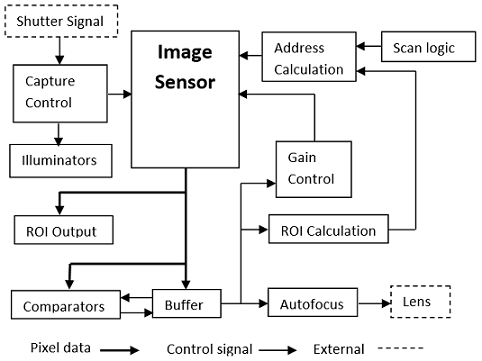
\includegraphics[width=6cm]{w_09_2018_Kharkevich1.png}
  \caption{Блок-схема примерной системы распознавания РОГ}
  \label{fig:Kharkevich1}
\end{figure}
\end{center} 

Программное обеспечение, реализующее алгоритм идентификации (\ref{fig:Kharkevich2}), логически разбивается на два блока: блок обработки изображения и блок взаимодействия с базой данных.

Блок обработки изображения получает несколько изображений глаза с монохромной камеры, выбирает лучшее из них и разбивает его на набор контрольных точек. Для этого используется алгоритмом обнаружения объектов на изображении   детектор на базе каскада хааровских классификаторов (метод Виолы-Джонса).

После получения контрольных точек обязательным этапом работы является \textbf{обучение классификатора}. К сожалению, при данном алгоритме скорость обучения очень медленная (при больших объемах обучающей выборки), но результаты поиска контрольных областей на изображении очень быстры. В качестве классификаторов были выбраны уже обученные каскады из \textbf{библиотеки OpenCV haarcascade\_eye.xml}.

OpenCV представляет собой простую в использовании библиотеку компьютерного зрения с более чем 500-ми функциями, способными работать в реальном времени. Фактически, OpenCV~--- это набор типов данных, функций и классов для обработки изображений алгоритмами компьютерного зрения.
\begin{center}
\begin{figure}[h!]
  \centering
  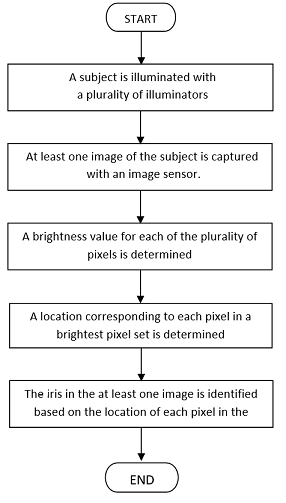
\includegraphics[width=6cm]{w_09_2018_Kharkevich2.png}
  \caption{Блок-схема алгоритма работы системы} 
  \label{fig:Kharkevich2}
\end{figure}
\end{center} 

Классификаторы часто неправильно классифицируют брови как глаза или не могут обнаружить глаза, когда освещение не очень хорошее. Также глаза, принадлежащие одному человеку, отличаются друг от друга, поэтому классификатор обучается отдельно для каждого глаза. Брови также включены в цель для обучения (\ref{fig:Kharkevich3}).

Для каждого глаза использовались собственные классификаторы OpenCV:
\begin{itemize}
\item левый глаз: \textbf{haarcascade\_lefteye\_2splits.xml}
\item правый глаз: \textbf{haarcascade\_righteye\_2splits.xml}
\end{itemize}
В ходе выполненных исследований и практических разработок, в том числе при реализации прикладного программного обеспечения, был использован комплекс средств разработки Qt 5.3.2 (GCC 4.9.2) для Linux Debian, в который входят библиотеки классов C++ версии 4.7.0, а также среда разработки, предназначенная для редактирования, компиляции и отладки кода~--- Qt Creator IDE версии 3.2.1.

\begin{center}
\begin{figure}[h!]
  \centering
  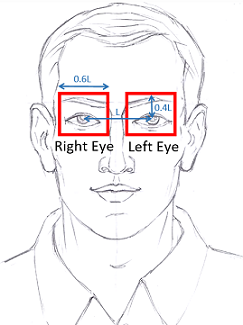
\includegraphics[width=6cm]{w_09_2018_Kharkevich3.png}
  \caption{Связь между расположением зрачков и областями глаз}
  \label{fig:Kharkevich3}
\end{figure}
\end{center} 

\subsection*{Идентификация по базе}
В процессе распознавания сравнивается полученный набор контрольных точек с записями, хранящимися в базе. В качестве метрики выбирается стандартное евклидово расстояние. При нахождении соответствующей записи программное средство определяет уровень доступа, которым обладает пользователь. Современное программное средство обеспечивает скорость сравнения примерно 300-500 мс.

\subsection*{Сканирование РОГ с помощью смартфона}
Благодаря быстрому развитию технологий смартфон стал оснащен высококачественной камерой и мощным процессором, что обеспечивают простой захват биометрического идентификатора \textbf{без дополнительного позиционирования положения глаз пользователя}. Для корректной работы данной технологии необходимо получение качественных фотографий. Камера современного смартфона изначально не приспособлена для целей идентификации личности, в связи с чем основной задачей ПО является подготовка и оптимизация начального изображения, используемого для анализа (подбор яркости, контраста и других параметров изображения).

\textbf{Устройство формирования изображения РОГ в смартфоне, содержащие датчик изображения и оптический узел} ~\cite{Kharkevich-3}, имеет два аппаратных блока: блок формирования изображения 102 и блок обработки 104 (\ref{fig:Kharkevich4})

\begin{center}
\begin{figure}[h!]
  \centering
  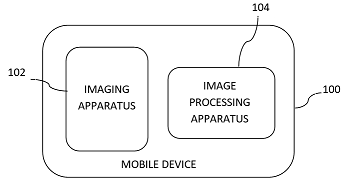
\includegraphics[width=6cm]{w_09_2018_Kharkevich4.png}
  \caption{Дополнительные блоки смартфона}
  \label{fig:Kharkevich4}
\end{figure}
\end{center} 

Блок формирования изображения формирует набор изображений, основанных на кадрах снятого видео или на наборе фотографий, и передает данный набор устройству обработки изображений. Блок обработки изображений выбирает наиболее четкое изображение и анализирует его. Алгоритм блока обработки изображений собирает контрольные точки с анализируемого изображения и сравнивает их с уже ранее обработанными изображениями «шаблонами», что в свою очередь позволяет идентифицировать объект по РОГ.
Следует отметить, что показанная схема опциональна и может содержать ряд дополнительных блоков, которые могут располагаться как непосредственной в смартфоне, так и быть отдельными устройствами, подключаемыми к нему.

\subsection*{Вывод}
Несмотря на потенциал метода среди различных биометрических систем, тормозящим фактором остается его высокая стоимость. Однако, постоянные исследования и разработки позволят снизить затраты на оборудование (применяя смартфоны для захвата и обработки радужной оболочки), возможностью использования библиотек компьютерного зрения с открытым исходным кодом OpenCV, а также расширение сферы использования за счет госзаказов~--- позволит технологии аутентификации по РОГ занять заметный сегмент на рынке биометрических систем контроля и управления доступом.

\begin{thebibliography}{9}
\bibitem{Kharkevich-1} Старовойтов, В.В. Распознавание человека по изображению радужной оболочки глаза: проблемы и достижения / В.В. Старовойтов, Ю.И. Монич // Искусственный интеллект.~--- 2011.~--- № 3.~--- с.278-284.
\bibitem{Kharkevich-2} Image sensor with integrated region of interest calculation for iris capture, autofocus and gain control: пат. США 9,514,365 / M.Tinker, D.A. Ackerman; опубл. 06.12.16 // Портал патентного ведомства США [Электронный ресурс].~--- Режим доступа: \url{https://www.uspto.gov/}.~--- Дата доступа 15.12.2017
\bibitem{Kharkevich-3} Iris imaging apparatus and methods for configuring an iris imaging apparatus: пат.США 9,366,843 / S.Prabhakar, V.Dvorovkin; опубл. 14.06.16 // Портал патентного ведомства США [Электронный ресурс].~--- Режим доступа: \url{https://www.uspto.gov/}.~--- Дата доступа 20.12.2017
\end{thebibliography}
\end{document}

\documentclass[10pt, a5paper]{article}
\usepackage{pdfpages}
\usepackage{parallel}
\usepackage[T2A]{fontenc}
\usepackage{ucs}
\usepackage[utf8x]{inputenc}
\usepackage[polish,english,russian]{babel}
\usepackage{hyperref}
\usepackage{rotating}
\usepackage[inner=2cm,top=1.8cm,outer=2cm,bottom=2.3cm,nohead]{geometry}
\usepackage{listings}
\usepackage{graphicx}
\usepackage{wrapfig}
\usepackage{longtable}
\usepackage{indentfirst}
\usepackage{array}
\newcolumntype{P}[1]{>{\raggedright\arraybackslash}p{#1}}
\frenchspacing
\usepackage{fixltx2e} %text sub- and superscripts
\usepackage{icomma} % коскі ў матэматычным рэжыме
\PreloadUnicodePage{4}

\newcommand{\longpage}{\enlargethispage{\baselineskip}}
\newcommand{\shortpage}{\enlargethispage{-\baselineskip}}

\def\switchlang#1{\expandafter\csname switchlang#1\endcsname}
\def\switchlangbe{
\let\saverefname=\refname%
\def\refname{Літаратура}%
\def\figurename{Іл.}%
}
\def\switchlangen{
\let\saverefname=\refname%
\def\refname{References}%
\def\figurename{Fig.}%
}
\def\switchlangru{
\let\saverefname=\refname%
\let\savefigurename=\figurename%
\def\refname{Литература}%
\def\figurename{Рис.}%
}

\hyphenation{admi-ni-stra-tive}
\hyphenation{ex-pe-ri-ence}
\hyphenation{fle-xi-bi-li-ty}
\hyphenation{Py-thon}
\hyphenation{ma-the-ma-ti-cal}
\hyphenation{re-ported}
\hyphenation{imp-le-menta-tions}
\hyphenation{pro-vides}
\hyphenation{en-gi-neering}
\hyphenation{com-pa-ti-bi-li-ty}
\hyphenation{im-pos-sible}
\hyphenation{desk-top}
\hyphenation{elec-tro-nic}
\hyphenation{com-pa-ny}
\hyphenation{de-ve-lop-ment}
\hyphenation{de-ve-loping}
\hyphenation{de-ve-lop}
\hyphenation{da-ta-ba-se}
\hyphenation{plat-forms}
\hyphenation{or-ga-ni-za-tion}
\hyphenation{pro-gramming}
\hyphenation{in-stru-ments}
\hyphenation{Li-nux}
\hyphenation{sour-ce}
\hyphenation{en-vi-ron-ment}
\hyphenation{Te-le-pathy}
\hyphenation{Li-nux-ov-ka}
\hyphenation{Open-BSD}
\hyphenation{Free-BSD}
\hyphenation{men-ti-on-ed}
\hyphenation{app-li-ca-tion}

\def\progref!#1!{\texttt{#1}}
\renewcommand{\arraystretch}{2} %Іначай формулы ў матрыцы зліпаюцца з лініямі
\usepackage{array}

\def\interview #1 (#2), #3, #4, #5\par{

\section[#1, #3, #4]{#1 -- #3, #4}
\def\qname{LVEE}
\def\aname{#1}
\def\q ##1\par{{\noindent \bf \qname: ##1 }\par}
\def\a{{\noindent \bf \aname: } \def\qname{L}\def\aname{#2}}
}

\def\interview* #1 (#2), #3, #4, #5\par{

\section*{#1\\{\small\rm #3, #4. #5}}

\def\qname{LVEE}
\def\aname{#1}
\def\q ##1\par{{\noindent \bf \qname: ##1 }\par}
\def\a{{\noindent \bf \aname: } \def\qname{L}\def\aname{#2}}
}

\begin{document}
\title{Системы распознавания речи с открытым исходным кодом\footnote{\url{daniil.boyko.2017@gmail.com}, \url{https://lvee.org/en/abstracts/273}}}
\author{Даниил Бойко, Минск, Belarus}
\maketitle
\begin{abstract}
We provide brief overview and comparison of  three open-source speech-recognition systems: CMUSphinx, Kaldi, DeepSpeech.  
\end{abstract}
\subsection*{Введение}

Сейчас существует огромное разнообразие коммерческих систем распознавания речи:

\begin{itemize}
  \item Google
  \item Amazon Alexa
  \item IBM Watson
  \item Siri
  \item Yandex
\end{itemize}

Они часто свободны для использования и предлагают открытые API (ссылки). Качество распознавания такими системами тоже довольно высокое. Какие же у них есть недостатки и зачем возится с системами с открытыми исходниками?

\begin{itemize}
  \item Перечисленные выше системы работают через интернет, соответственно, если нет сети они не работают
  \item Нет пользовательского контроля: как мы увидим, качество распознавания зависит от используемой языковой модели (в разных контекстах разная вероятность разных слов, etc). Стандартные системы используют усредненную модель языка, либо модель, разработанную для их задач, а не для наших
  \item Пересылка данных через сеть может вносить большие задержки при плохом качестве связи
  \item Проблемы с приватностью
\end{itemize}

В этом докладе мы рассмотрим три свободные системы распознавания речи и попробуем сравнить их качество:

\begin{enumerate}
  \item CMU Sphinx
  \item Kaldi
  \item Mozilla DeepSpeech
\end{enumerate}

\subsection*{CMU Sphinx}

CMU Sphinx (если кратко, то просто Sphinx)~--- группа систем распознавания речи разработанных университетом Карнеги Меллон. Она включает в себя серию систем распознавания (Sphinx 2~--- 4) и акустическую тренировочную модель (SphinxTrain).

В 2000 компонент системы распознавания речи Sphinx 2 был опубликован как открытый код, а в 2001 компонент Sphinx 3. На данный момент активно разрабатывается Sphinx 4 (написанный на Java, удобный для встраивания в серверные системы) и\linebreak PocketSphinx (написанный на C и удобный для встраиваемых систем). Распространяется под лицензией BSD.

В этом докладе мы будем в основном рассматривать\linebreak PocketSphinx.

\subsubsection*{Установка}

Pocketsphinx доступен в качестве пакета в большинстве линуксов. 
Для работы ему также необходимы файлы языковой модели, файлы акустической модели и словарь произношения (фонетический словарь).

\textbf{Акустическая модель}~--- задает способ отображения потока речи (представленных так называемыми кепстральными коэффициентами ) в фонемы (обозначения звуков речи, которые используются в словарях произношения). В pocketsphinx используются скрытые марковские модели (HMM) в качестве акустической модели.

\textbf{Словарь произношения}~--- содержит транскрипцию произношения слов. Отображает слово в набор фонем.

\textbf{Языковая модель}~--- задает вероятности разных слов и словосочетаний, которые будут встречаться в произносимом тексте. Очень сильно зависит от тематики текста.

Для английского языка языковые модели доступны из дистрибутива. Для большинства других языков (в т.ч.  и для русского) файлы языковой, акустической модели и словари доступны на \url{http://www.voxforge.org}.

\subsubsection*{Запуск}

С командной строки запускается так (онлайновый режим, работа с микрофона):

\verb@ALSA_OSS_PCM_DEVICE="hw:CARD=MS,DEV=0" aoss pocketsphinx_@
\verb@continuous -hmm ru-RU-adapt/ -dict msu_ru_nsh.dic -lm <some@
\verb@ language model>  -inmic yes@

\verb@-hmm задает путь к директории акустической модели@

\verb@-lm путь к языковой модели@

\verb@-dict путь к словарю произношения@

Оффлайновый режим (транскрипция текста, запуск на wav файле):

\verb@pocketsphinx_continuous -infile sample.wav > decode.txt@

\subsection*{Kaldi}

Kaldi~--- это набор инструментов для распознавания речи, написанный на языке C++, имеющий лицензию Apache v2.0. В больше степени Kaldi предназначена для исследования распознавания речи.

Одной из целью Kaldi было иметь современный и гибкий код, написанный на C++, который можно было бы легко расширять и изменять.

Kaldi включает следующие возможности:

\begin{itemize}
  \item Обширная поддержка линейной алгебры~--- включена матричная библиотека, которая оборачивает стандартные процедуры BLAS и LAPACK.
  \item Расширяемая конструкция~--- алгоритмы написаны наиболее универсальным способом.
  \item Открытая лицензия~--- код находится под лицензией Apache 2.0 которая является одной из наименее ограничительных лицензий.
  \item Полные рецепты~--- цель Kaldi предоставить полные рецепты построения систем распознавания речи, которые работают из широко доступных баз данных. Это важный аспект Kaldi, так как код публично доступен под лицензией, которая разрешает изменения и переиздание. Kaldi призывает людей выпускать свой код вместе с каталогом скриптов аналогично тому, как делает сама Kaldi
\end{itemize}

Некоторые особенности системы Kaldi:

\begin{itemize}
  \item Код Kaldi весь или почти весь тщательно оттестирован
  \item Код Kaldi легок для понимания~--- несмотря на то что инструментарий Kaldi очень большой, разработчики старались, чтобы каждую часть кода можно было бы разобрать без особых усилий. Некоторые участки кода дублировались специально для того, чтобы код был понятнее.
  \item Код Kaldi легко использовать повторно и рефакторить~--- разработчики старались сделать код настолько менее связным на сколько это возможно. В общем случае это значит, что какой-либо файл содержит директив \#include настолько мало, на сколько это возможно.
  \item Сейчас Kaldi содержит скрипты для большинства стандартных задач.
\end{itemize}

\subsubsection*{Установка}

\verb@Git clone https://github.com/kaldi-asr/kaldi@

В склонированном репозитории есть файл INSTALL, который содержит инструкции по компиляции в нем написано следующее:

\begin{enumerate}
  \item go to tools/  and follow INSTALL instructions there.
  \item go to src/ and follow INSTALL instructions there.
\end{enumerate}

\subsubsection*{Запуск}

Вместе с системой распознавания Kaldi предоставляет большое количество примеров использования системы. Все примеры находится в папке egs.

Оффлайновый режим (транскрипция текста, запуск на wav файле):

Есть специальный скрипт в примерах, который предназначен для распознавания wav файла. Он находится по следующему пути: \url{egs/apiai\_decode/s5/recognize-wav.sh}. Для распознавания этот скрипт запускается передавая ему путь к wav файлу. Например:

\verb@./recognize-wav.sh sample.wav@

\subsection*{Mozilla DeepSpeech}

DeepSpeech~--- это движок с открытым исходным кодом, для преобразования речи в текст. Для обучения используются модель, обученную методами машинного обучения, на основе глубоких речевых исследованиях Байду. DeepSpeech использует проект TensorFlow чтобы облегчить реализацию

\subsubsection*{Установка}

Весь проект находится на github по адресу: \url{https://github.com/mozilla/DeepSpeech#getting-the-pre-trained-model}

Для того, чтобы установить:
\verb@pip install deepspeech@
или
				
\verb@pip install deepspeech-gpu@
или
	
\verb@git clone https://github.com/mozilla/DeepSpeech@

Скачиваем модель для распознавания:
wget -O~--- 

\verb@https://github.com/mozilla/DeepSpeech/releases/download/@

\verb@v0.1.1/deepspeech-0.1.1-models.tar.gz | tar xvfz -@

\subsubsection*{Запуск}

Оффлайновый режим (транскрипция текста, запуск на wav файле):

\verb@deepspeech models/output_graph.pb my_audio_file.wav @
 
\verb@models/alphabet.txt@

\subsection*{Сравнение систем}

\subsubsection*{Метрики качества}

WER~--- это производная от величины называемой «расстояние Левенштейна», которая вычисляется на уровне слов, а не на уровне фонем. Расстояние Левенштейна~--- это минимальное количество операций вставки одного символа, удаления одного символа и замены одного символа на другой, необходимых для превращения одной строки в другую.

\verb@WER = (S + D + I)/N = (S + D + I)/(S + D + C)@

\begin{itemize}
  \item S~--- число операций замены слов
  \item D~--- число операций удаления слов
  \item I~--- число операций вставки слов
  \item C~--- количество правильно распознанных слов
  \item N~--- общее количество слов
\end{itemize}

SER~--- это общая метрика для определения точности системы распознавания. SER представляет собой показатель отношения количества неправильно распознанных предложений к количеству всех предложений.

\verb@SER = Sв / S@

\begin{itemize}
  \item Sв~--- количество предложений распознанных без ошибок
  \item S~--- общее количество предложений
\end{itemize}

SF~--- это общая метрика для определения скорости распознавания системы. SF представляет собой показатель отношения времени распознавания к длительности распознаваемого сигнала.

\verb@SF = Tрасп / T@

\begin{itemize}
  \item Tрасп~--- время распознавания сигнала
  \item T~--- длительность, измеряется в долях реального времен
\end{itemize}

\subsubsection*{Результаты сравнений}

Результаты сравнений приведены в следующей таблице.

%\begin{turn}{90} 
%\usepackage{array}
\newcolumntype{L}[1]{>{\raggedright\let\newline\\\arraybackslash\hspace{0pt}}m{#1}}
\centering
\begin{table}
  \begin{tabular}{|L{2cm}|L{3cm}|L{2cm}|L{2cm}|}
\hline      & CMU~Sphinx ~ (pocketsphinx)  & Kaldi  & DeepSpeech  \\ \hline
%      &   &   &   \\
     \textbf{WER, \%}  &  42.01  &  22.81  &  29.96  \\ \hline
     \textbf{SER, \%}  &  84.24  &  76.00  &  84.00  \\ \hline
     \textbf{SF, \%}  &  34.83  &  149.31  &  215.65  \\ \hline
     \textbf{Язык}  &  C/Java  &  C++  &  Python  \\ \hline
     \textbf{Структура}  &  Модульная  &  Модульная  &  Модульная  \\ \hline
     \textbf{Документа\-ция}  &  Подробная онлайн-документация, видео-уроки на YouTube  &  Подробная онлайн-документация  &  Подробная онлайн-документация  \\ \hline
     \textbf{Поддержи\-ваемые
ОС}  &  Linux, Mac OS, Windows, Android  &  Linux, Windows  &  Linux, Mac OS,
Windows, Android  \\ \hline
     \textbf{Интерфейс}  &  Консольный, API  &  Консольный  &  Консольный  \\ \hline
     \textbf{Языки}  &  Множество языков, в т.\,ч. экзотические  &  Английский  &  Английский  \\ \hline
     \textbf{Лицензия}  &  BSD  &  Apache v2.0 (BSD-подобная)  &  Mozilla Public License 2.0 (BSD-подобная)  \\ \hline
 \end{tabular}
\end{table}
%\end{turn}
 

\end{document}
 
 
\documentclass[10pt, a5paper]{article}
\usepackage{pdfpages}
\usepackage{parallel}
\usepackage[T2A]{fontenc}
\usepackage{ucs}
\usepackage[utf8x]{inputenc}
\usepackage[polish,english,russian]{babel}
\usepackage{hyperref}
\usepackage{rotating}
\usepackage[inner=2cm,top=1.8cm,outer=2cm,bottom=2.3cm,nohead]{geometry}
\usepackage{listings}
\usepackage{graphicx}
\usepackage{wrapfig}
\usepackage{longtable}
\usepackage{indentfirst}
\usepackage{array}
\newcolumntype{P}[1]{>{\raggedright\arraybackslash}p{#1}}
\frenchspacing
\usepackage{fixltx2e} %text sub- and superscripts
\usepackage{icomma} % коскі ў матэматычным рэжыме
\PreloadUnicodePage{4}

\newcommand{\longpage}{\enlargethispage{\baselineskip}}
\newcommand{\shortpage}{\enlargethispage{-\baselineskip}}

\def\switchlang#1{\expandafter\csname switchlang#1\endcsname}
\def\switchlangbe{
\let\saverefname=\refname%
\def\refname{Літаратура}%
\def\figurename{Іл.}%
}
\def\switchlangen{
\let\saverefname=\refname%
\def\refname{References}%
\def\figurename{Fig.}%
}
\def\switchlangru{
\let\saverefname=\refname%
\let\savefigurename=\figurename%
\def\refname{Литература}%
\def\figurename{Рис.}%
}

\hyphenation{admi-ni-stra-tive}
\hyphenation{ex-pe-ri-ence}
\hyphenation{fle-xi-bi-li-ty}
\hyphenation{Py-thon}
\hyphenation{ma-the-ma-ti-cal}
\hyphenation{re-ported}
\hyphenation{imp-le-menta-tions}
\hyphenation{pro-vides}
\hyphenation{en-gi-neering}
\hyphenation{com-pa-ti-bi-li-ty}
\hyphenation{im-pos-sible}
\hyphenation{desk-top}
\hyphenation{elec-tro-nic}
\hyphenation{com-pa-ny}
\hyphenation{de-ve-lop-ment}
\hyphenation{de-ve-loping}
\hyphenation{de-ve-lop}
\hyphenation{da-ta-ba-se}
\hyphenation{plat-forms}
\hyphenation{or-ga-ni-za-tion}
\hyphenation{pro-gramming}
\hyphenation{in-stru-ments}
\hyphenation{Li-nux}
\hyphenation{sour-ce}
\hyphenation{en-vi-ron-ment}
\hyphenation{Te-le-pathy}
\hyphenation{Li-nux-ov-ka}
\hyphenation{Open-BSD}
\hyphenation{Free-BSD}
\hyphenation{men-ti-on-ed}
\hyphenation{app-li-ca-tion}

\def\progref!#1!{\texttt{#1}}
\renewcommand{\arraystretch}{2} %Іначай формулы ў матрыцы зліпаюцца з лініямі
\usepackage{array}

\def\interview #1 (#2), #3, #4, #5\par{

\section[#1, #3, #4]{#1 -- #3, #4}
\def\qname{LVEE}
\def\aname{#1}
\def\q ##1\par{{\noindent \bf \qname: ##1 }\par}
\def\a{{\noindent \bf \aname: } \def\qname{L}\def\aname{#2}}
}

\def\interview* #1 (#2), #3, #4, #5\par{

\section*{#1\\{\small\rm #3, #4. #5}}

\def\qname{LVEE}
\def\aname{#1}
\def\q ##1\par{{\noindent \bf \qname: ##1 }\par}
\def\a{{\noindent \bf \aname: } \def\qname{L}\def\aname{#2}}
}

\switchlang{en}
\begin{document}
\title{How open source changing and reshaping enterprises\footnote{\url{andreyrom@tut.by}, \url{https://lvee.org/en/abstracts/285}}}
\author{Андрей Романюк, Minsk, Belarus}
\maketitle
\begin{abstract}
Since the past 25 years relationship between open source and enterprise changed dramatically. While in the middle of 1990s open source was considered as a hobby for enthusiasts these days most enterprises build their success using open source products. There are three major trends that changed the shape of open source and enterprise relationship over the time 1. enterprise compatibility - we can see a lot of successful open source products used to leverage the business of enterprise products. Among them we can see NGINX, RedHat, etc\ldots 2. product innovation cycle for enterprise software is still stuck on 3 years while open source products have much more agile approach delivering\linebreak innovative releases much more frequently 3. platform compatibility is the major differentiator between open source and closed source platforms. Open source software helps users to use their products across multiple platforms while closed source application try to stick user on a single platform. The level of integration and trust between enterprise solutions and open source products grows every year. Future innovations and successful businesses start today with help of open source.
\end{abstract}

It is obvious that for enterprises the future is built on open source. In the last 10 years any innovation adopted in the enterprises has had its roots in open source. Cloud computing, containers, databases, new languages (node JS and GO)~--- they all start in open source. And enterprises starting to listen, they starting to embrace open source. Red Hat claims that 90\% of fortune 500 are using Red Hat products and services. That was unheard 25 years ago.

Let’s look at 3 major trends that shape the changes between\linebreak enterprise and open source in the last 2 decades.

\subsection*{Enterprise compatibility}

What was enterprise compatibility 25 years ago? 25 years is important because at this time enterprises started adopting open source.

OpenSource products started finding their users because they solved real problems. At the same time closed source companies tried to block open source solutions trying to communicate the main objection: open source is risky, and it is not enterprise ready.

There are many amazing quotes from this time about open source. Bill Gates from Microsoft said: <<Open Source is good for hobbies and enthusiasts\ldots>>. It was also famously said that the open source is like a free puppy, you’ve got this puppy home, you’ve got to feed it, you’ve got to train it and then you’ve got to clean up after it. But, guess what, we took that puppy home, and that puppy grew up to be a wolf, that’s got teeth and claws, and it’s got sights sit firmly on enterprise software. And it’s not going to stop.

25 years later open source is enterprise compatible. Everything has changed and enterprises now have choice that they never had before. Now the companies like NGINX propose the products available with open source, package, fully backed up with professional services, training, tested and supported. There are more things available 
\begin{itemize}
\item Army of developers and community that grew up with open source
\item open source is now proven, ready and nothing is going to stop it
\item open source now is less risky than closed source (some examples with NGINX and other software)
\end{itemize}

\subsection*{Product and innovation cycle}

Closed source is still stuck in 3 years product cycle (example~--- MS Office~--- known as a train that always arrives every three years). It is great for license renewals, its good for maximizing amount of money you can get from your customers, but lousy for delivering innovation.
 
Open source community believes that 3 years are too long to wait for innovation. Innovation is not happening in 3 year cycles, it is happening now. Open source approach is fundamentally different then the closed source. It encapsulates instant feedback from multiple sources~---\linebreak amateurs, professionals, students, engineers, architects, individual development companies, startups, midsize companies, enterprises, largest internet giants all over the world and delivers the changes very quickly. New ideas become materialized to the new projects, they are quickly released into the staging and stable branches at the speed enterprises are asking about it.

\subsubsection*{Platforms compatibility}

New technologies are getting more complex and the enterprises looking for the platforms to simplify this and to reduce risk. They see it like a set of the best practices and patterns and software that works better together. And the challenge with the closed source platforms is that you are always locked in. Closed source has to protect their intellectual property, their own developers, their own engineers being tainted by other peoples IP. Fundamentally they try to lock their customers to their platform (example iTunes that don’t support Android users). This kind of lock in creates hostages, not happy\linebreak customers.
 
Open source suggests fundamentally different approach over the platforms~--- it integrates with various platforms and this is part of DNA of OpenSource solutions. For example NGINX is supported on AWS, Azure, GCP, kubernetes; on premise, private cloud, containers, hybrid cloud, any kind of cloud that you want. Platform should free you, but not lock you in. 
Open source is a better way to deliver the software.

Now let’s see some examples how open source products help driving the business of the large corporations. 

I have experience working in well known producer of the network equipment from California Netgear Inc. This company is known more than 20 years for their famous network devices: routers, wi-fi access points, bridges and other equipment. When we take Netgear router and look to the basic firmware components of this device we can see that it uses linux kernel, major libraries: curl, openssl, gsoap. And there are UI modules Node JS, Angular JS, Apache and other components to organize effective user interface. Server side components include Spring framework, Tomcat, NGINX, MySQL, Redis and many more.

Another company that we can look at is ARLO Inc~--- the leading expert in cloud video systems. ARLO is located in USA, California and having more than 50\% of US market. Their solutions – cloud video systems embed wide range of open source products such as Busybox, uClibc, GCC tools, Open SSL \& TLS, libcurl, libjson and many others. Together these tools help defining the shape of the final product and create that amazing user experience that makes those enterprise\linebreak successful.

Both ARLO and Netgear are examples of how successful business can leverage its own enterprise products by using open source\linebreak technologies. The very possibility of using so many open source projects in an enterprise solution is a great indicator of maturity of open source.

If 20 years ago the company had to build the most part of its enterprise value from scratch, now the most efforts are put into the building the product from various blocks provided by open source\linebreak community.

Today we can say for sure that the future of software development is with open source.
 

\end{document}

\documentclass[10pt, a5paper]{article}
\usepackage{pdfpages}
\usepackage{parallel}
\usepackage[T2A]{fontenc}
\usepackage{ucs}
\usepackage[utf8x]{inputenc}
\usepackage[polish,english,russian]{babel}
\usepackage{hyperref}
\usepackage{rotating}
\usepackage[inner=2cm,top=1.8cm,outer=2cm,bottom=2.3cm,nohead]{geometry}
\usepackage{listings}
\usepackage{graphicx}
\usepackage{wrapfig}
\usepackage{longtable}
\usepackage{indentfirst}
\usepackage{array}
\newcolumntype{P}[1]{>{\raggedright\arraybackslash}p{#1}}
\frenchspacing
\usepackage{fixltx2e} %text sub- and superscripts
\usepackage{icomma} % коскі ў матэматычным рэжыме
\PreloadUnicodePage{4}

\newcommand{\longpage}{\enlargethispage{\baselineskip}}
\newcommand{\shortpage}{\enlargethispage{-\baselineskip}}

\def\switchlang#1{\expandafter\csname switchlang#1\endcsname}
\def\switchlangbe{
\let\saverefname=\refname%
\def\refname{Літаратура}%
\def\figurename{Іл.}%
}
\def\switchlangen{
\let\saverefname=\refname%
\def\refname{References}%
\def\figurename{Fig.}%
}
\def\switchlangru{
\let\saverefname=\refname%
\let\savefigurename=\figurename%
\def\refname{Литература}%
\def\figurename{Рис.}%
}

\hyphenation{admi-ni-stra-tive}
\hyphenation{ex-pe-ri-ence}
\hyphenation{fle-xi-bi-li-ty}
\hyphenation{Py-thon}
\hyphenation{ma-the-ma-ti-cal}
\hyphenation{re-ported}
\hyphenation{imp-le-menta-tions}
\hyphenation{pro-vides}
\hyphenation{en-gi-neering}
\hyphenation{com-pa-ti-bi-li-ty}
\hyphenation{im-pos-sible}
\hyphenation{desk-top}
\hyphenation{elec-tro-nic}
\hyphenation{com-pa-ny}
\hyphenation{de-ve-lop-ment}
\hyphenation{de-ve-loping}
\hyphenation{de-ve-lop}
\hyphenation{da-ta-ba-se}
\hyphenation{plat-forms}
\hyphenation{or-ga-ni-za-tion}
\hyphenation{pro-gramming}
\hyphenation{in-stru-ments}
\hyphenation{Li-nux}
\hyphenation{sour-ce}
\hyphenation{en-vi-ron-ment}
\hyphenation{Te-le-pathy}
\hyphenation{Li-nux-ov-ka}
\hyphenation{Open-BSD}
\hyphenation{Free-BSD}
\hyphenation{men-ti-on-ed}
\hyphenation{app-li-ca-tion}

\def\progref!#1!{\texttt{#1}}
\renewcommand{\arraystretch}{2} %Іначай формулы ў матрыцы зліпаюцца з лініямі
\usepackage{array}

\def\interview #1 (#2), #3, #4, #5\par{

\section[#1, #3, #4]{#1 -- #3, #4}
\def\qname{LVEE}
\def\aname{#1}
\def\q ##1\par{{\noindent \bf \qname: ##1 }\par}
\def\a{{\noindent \bf \aname: } \def\qname{L}\def\aname{#2}}
}

\def\interview* #1 (#2), #3, #4, #5\par{

\section*{#1\\{\small\rm #3, #4. #5}}

\def\qname{LVEE}
\def\aname{#1}
\def\q ##1\par{{\noindent \bf \qname: ##1 }\par}
\def\a{{\noindent \bf \aname: } \def\qname{L}\def\aname{#2}}
}

\switchlang{ru}
\begin{document}
\title{Автоматизированный поиск багов в C/C++\footnote{\url{zamazan4ik@tut.by}, \url{https://lvee.org/en/abstracts/279}}}
\author{Александр Зайцев, Минск, Belarus}
\maketitle
\begin{abstract}
Nowadays programs are too complex for verification and any developer can't guarantee that program is valid in every situation. Inthis talk I'll try to introduce modern ways for automatic testing C/C++ programs. I will talk about proper compiler settings, static and dynamic analyzers, sanitizers and fuzzing tecniques.
\end{abstract}

Сегодня хотелось бы рассказать о такой вещи как фаззинг\linebreak (fuzzing) тестирование и чем оно будет полезно как для разработчиков программ, так и для их мейнтейнеров в различных дистрибутивах. Так как я в основном пользуюсь в своей работе языком программирования C++, то я буду рассказывать про фаззинг в контексте разработки на данном языке программирования (Си тоже касается :)

\subsection*{Почему эти языки находятся в зоне риска?}

Языки программирования C/C++ заточены на производительность. За это приходится платить тем, что в ходе работы программы отсутствуют многие элементарные проверки валидности программы. Даже банальный выход за пределы массива или разыменование нулевого указателя ведёт не к исключению, а к так называемому <<неопределённому поведению>>, которое позволяет компилятору творить с вашей программой всё что угодно (читать как <<программа становится автоматически невалидной>>).

\subsection*{Типичные примеры неопределённого поведения:}
\begin{itemize}
\item Разыменование нулевого указателя
\item Использование невалидного указателя\textbackslash{}итератора\textbackslash{}ссылки
\item Переполнение знаковых переменных
\item Нарушение контрактов стандартных алгоритмов
\item Многократное освобождение памяти
\item Использование памяти после освобождения
\end{itemize}
Как будем бороться с этим?

\subsection*{Настройка компилятора}
\begin{itemize}
\item Включение как можно большего числа предупреждений (аккуратнее на грязной кодовой базе, а то есть шанс утонуть)
\item Обновляйте компиляторы по возможности~---новые компиляторы~---новые предупреждения и диагностики
\item Для поддержания чистоты~---pedantic, чтобы неповадно было игнорировать предупреждения
\end{itemize}
\subsection*{Статический анализ кода}

Когда нам мало диагностик компилятора, на помощь нам могут прийти такие средства как статические анализаторы кода. В них обычно реализовано гораздо больше проверок на типичные ошибки разработчика, нежели в компиляторах (на то они и есть специализированные средства). Рекомендуемые к использованию статические анализаторы кода:
\begin{itemize}
\item cppcheck (GPL-3.0)
\item Clang-Tidy (BSD)
\item (не уверен, что стоит называть проприетарные средства тут)
\end{itemize}
Вкупе с компиляторами большУю часть ошибок можно отсеять ещё до запуска самой программы только путём анализа исходных файлов.

\subsection*{Санитайзеры}

Санитайзеры (sanitizers)~---утилиты из уже поставки компиляторов, которые помогают найти проблемы в вашем коде.
Санитайзеры бывают:
\begin{itemize}
\item Address~---помогает найти проблемы с памятью (утечка, двойное разыменование и т.д.). Работает как перехват всех операций с памятью и проверка \textbf{во время работы}. Значительное замедление работы
\item Thread~---помогает находить состояния гонки и deadlocks в вашем коде
\item Undefined~---помогает диагностировать неопределённое поведение в коде. Само собой разумеется, что он не может гарантированно найти все ошибки, потому что это C++.
\item CFE
\end{itemize}

Разработчики поопытнее ходят между граблей аккуратнее и с использованием специальных инструментов~---санитайзеров, но даже это их не спасает, так как с ростом размера программы сложно гарантировать её валидность в целом. Тестами всю систему в целом тоже очень и очень сложно покрыть. Можно к этому стремиться, но не всегда получается.

\subsection*{Альтернатива санитайзерам}

Можно для обнаружения проблем во время исполнения программы использовать Valgrind и построенные на его базе программы. Тут нам помогут программы DRD, Helgrind, Memcheck. Если Вы пользователь Windows, то для Вас альтернативой будет являться программа Dr. Memory. Лицензия Valgrind~---GPL-2.0, Dr. Memory~---LGPL.

\subsection*{Что такое фаззинг-тестирование?}

Грубо говоря, это вид тестирования, при котором на вход нашей программе подаётся огромное количество различных входных данных, после чего мы смотрим, как наша программа себя поведёт на них. В идеале, наша программа на корректных данных должна выдавать какой-либо корректный результат, а на некорректных завершаться каким-либо образом, который задумал автор. К сожалению, не всегда так происходит.

Рекомендуемые к использованию фаззеры: 
\begin{itemize}
\item AFL (Apache)
\item Libfuzzer (BSD)
\end{itemize}

\subsection*{Фаззинг и санитайзеры}

Так как фаззеры запускают нашу программу огромное количество раз на абсолютно разных данных, то очень хорошей идеей является запуск программы под фаззером и под санитайзером одновременно, так как таким образом увеличивается шанс нахождения какой-либо ошибки (утечки памяти, например), а то всё тоже является невалидным поведением.

\subsection*{Фаззинг для Open-Source}

Для тестирования Open-Source проектов Google сделал проект Oss-Fuzz. Это проект, который автоматически запускает программы с открытым исходным кодом под фаззерами на мощностях\linebreak Google. От проекта всего лишь требуется добавить свой проект в репозиторий, следовать довольно простым требованиям и дождаться одобрения от ребят из Google. И всё~---потом можно расслабиться и ждать отчётов с ошибками.

В целом это всё, что я хотел рассказать. Спасибо за внимание!

\end{document}

\documentclass[10pt, a5paper]{article}
\usepackage{pdfpages}
\usepackage{parallel}
\usepackage[T2A]{fontenc}
\usepackage{ucs}
\usepackage[utf8x]{inputenc}
\usepackage[polish,english,russian]{babel}
\usepackage{hyperref}
\usepackage{rotating}
\usepackage[inner=2cm,top=1.8cm,outer=2cm,bottom=2.3cm,nohead]{geometry}
\usepackage{listings}
\usepackage{graphicx}
\usepackage{wrapfig}
\usepackage{longtable}
\usepackage{indentfirst}
\usepackage{array}
\newcolumntype{P}[1]{>{\raggedright\arraybackslash}p{#1}}
\frenchspacing
\usepackage{fixltx2e} %text sub- and superscripts
\usepackage{icomma} % коскі ў матэматычным рэжыме
\PreloadUnicodePage{4}

\newcommand{\longpage}{\enlargethispage{\baselineskip}}
\newcommand{\shortpage}{\enlargethispage{-\baselineskip}}

\def\switchlang#1{\expandafter\csname switchlang#1\endcsname}
\def\switchlangbe{
\let\saverefname=\refname%
\def\refname{Літаратура}%
\def\figurename{Іл.}%
}
\def\switchlangen{
\let\saverefname=\refname%
\def\refname{References}%
\def\figurename{Fig.}%
}
\def\switchlangru{
\let\saverefname=\refname%
\let\savefigurename=\figurename%
\def\refname{Литература}%
\def\figurename{Рис.}%
}

\hyphenation{admi-ni-stra-tive}
\hyphenation{ex-pe-ri-ence}
\hyphenation{fle-xi-bi-li-ty}
\hyphenation{Py-thon}
\hyphenation{ma-the-ma-ti-cal}
\hyphenation{re-ported}
\hyphenation{imp-le-menta-tions}
\hyphenation{pro-vides}
\hyphenation{en-gi-neering}
\hyphenation{com-pa-ti-bi-li-ty}
\hyphenation{im-pos-sible}
\hyphenation{desk-top}
\hyphenation{elec-tro-nic}
\hyphenation{com-pa-ny}
\hyphenation{de-ve-lop-ment}
\hyphenation{de-ve-loping}
\hyphenation{de-ve-lop}
\hyphenation{da-ta-ba-se}
\hyphenation{plat-forms}
\hyphenation{or-ga-ni-za-tion}
\hyphenation{pro-gramming}
\hyphenation{in-stru-ments}
\hyphenation{Li-nux}
\hyphenation{sour-ce}
\hyphenation{en-vi-ron-ment}
\hyphenation{Te-le-pathy}
\hyphenation{Li-nux-ov-ka}
\hyphenation{Open-BSD}
\hyphenation{Free-BSD}
\hyphenation{men-ti-on-ed}
\hyphenation{app-li-ca-tion}

\def\progref!#1!{\texttt{#1}}
\renewcommand{\arraystretch}{2} %Іначай формулы ў матрыцы зліпаюцца з лініямі
\usepackage{array}

\def\interview #1 (#2), #3, #4, #5\par{

\section[#1, #3, #4]{#1 -- #3, #4}
\def\qname{LVEE}
\def\aname{#1}
\def\q ##1\par{{\noindent \bf \qname: ##1 }\par}
\def\a{{\noindent \bf \aname: } \def\qname{L}\def\aname{#2}}
}

\def\interview* #1 (#2), #3, #4, #5\par{

\section*{#1\\{\small\rm #3, #4. #5}}

\def\qname{LVEE}
\def\aname{#1}
\def\q ##1\par{{\noindent \bf \qname: ##1 }\par}
\def\a{{\noindent \bf \aname: } \def\qname{L}\def\aname{#2}}
}

\begin{document}
\title{Взгляд на перевод инфраструктуры на базе WIndows на Unix/LInux\footnote{\url{d.stepanov@itg.by}, \url{https://lvee.org/en/abstracts/274}}}
\author{Дмитрий Степанов, Минск, Belarus}
\maketitle
\begin{abstract}
This Engineering Report carries the essence of the problem, the integration between the two worlds and the camps of unqualified skeptics, who are often similar to the racetrack. 
The transition from a proprietary infrastructure to a free one at this given time will always be complicated by two factors -- maintenance and integration.
\end{abstract}
<<\ldots{}кто из вас без греха, первый брось в нее камень>>

\subsection*{Введение}

Развитие цифровых технологий с каждым годом предлагает, в потребительском плане, все более широкий спектр сервисов, программ, которые упрощают жизнедеятельность человека, ведение бизнеса предприятия и нашу жизнь в целом.

Компании малого и среднего бизнеса ищут решения, которые позволят идти в ногу с современными тенденциями в сфере IT технологий, новейшими программными разработками, и естественно чтобы последние не стали тяжкой ношей для развивающего предприятия.

Здесь рассматривается один из вариантов будущего систем, построенных на компромиссе между проприетарным программным обеспечением и продуктами, распространяющимися под лицензией GNU GPL или иными~--- варианты <<почти>> бесшовной миграции <<классической>> инфраструктуры на решения основанные на Linux.

Представленые материалы основаны исключительно на эмпирических методах внедрения решений на базе свободно распространяемого программного обеспечения в действующие инфраструктуры предприятий, и не несет в себе глобального решения проблемы.

По субъективному мнению автора, будущее СПО~--- за гибридизацией, между свободно распространяемым программным обеспечением и проприетарным.

\subsection*{Задача}

Первоначальной задачей, поставленной перед автором и его командой стали уменьшение стоимости обслуживания IT-\linebreak инфраструктуры предприятия без существенных потерь в сервисном эквиваленте и стоимости обслуживающего персонала (как обычно и происходит в случае внедрения Linux/Unix; опционально выделим GNU, так как многие приложения, распространяемые по данной философии, давно утратили суть).

Проще говоря, уже имеющийся на предприятии специалист должен в кратчайшие сроки и без особых трудностей освоить ново-внедряемые сервисы на базе Linux.

\subsection*{Действующая структура предприятия и принятые решения}

Существующие Сервисы (в рамках одного физического сервера): Active directory, DHCP, DNS, File Services, Gateway (на базе продуктов компании Kerio), сервер удалённого рабочего стола, 1С Бухгалтерия и некоторые иные сервисы, которые к сожалению в реалиях некоторых сфер бизнеса пока еще не могут быть интегрированы с системами на OPS (преимущественно программное обеспечение, выпущенное государственными органами~--- подача деклараций, таможня и многие иные).

Требуемое <<Заказчиком>> развитие:

\begin{itemize}
  \item максимальное уменьшение стоимость программного обеспечения;
  \item стоимость обслуживания инфраструктуры~--- по сути стоимость персонала.
\end{itemize}

Естественно, в большинстве случаев внедряемого OPS, большинство компаний, не относящихся к IT, останавливает стоимость специалиста, способного сопровождать инфраструктуру Linux/Unix, его замена, и многие иные аспекты, связанные с рыночной и <<привычной>> стороной вопроса.

Этапы:

\textbf{Этап 1}. Разделение существующей структуры на сегментированную структуру <<один сервис~--- один сервер>>.
Данное решение обусловлено необходимостью управлять каждым сервисом независимо от остальных, с минимальными вариациями простоя инфраструктуры в целом.

\textbf{Этап 2.} Подбор системы виртуализации на базе Open Source.
Рассматривались решения на базе KVM и XCP-ng, а так же вариация на базе VMware ESXi. Внедрение виртуализации~--- решение классическое, обусловленное необходимостью максимально (насколько возможно) использовать выделенные серверные мощности, упрощенное резервное копирование, быстротe и простотe запуска нового сервиса, оптимальное решение для реализации \textbf{этапа 1}.

Выбор был остановлен на XCP-ng, как на гипервизоре с хорошо продуманной простой установкой и настройкой и интерфейсом, близким для специалистов, которые работали в гипервизорах от компании VMware.

Также выбор пал на данный гипервизор после <<ловкого трюка>> со стороны компании Xen Citrix, которая урезала функционал гипервизора, распространяемого по лицензии GNU GPL. В частности, по этой же причине было принято решение не эксплуатировать гипервизор от компании VMware.

Так же развернутый для XCP-ng, Xen Orchestra позволяет проводить резервное копирование, строить базовые примитивы облака, что в свою очередь позволяет уменьшить необходимость взаимодействия неквалифицированного специалиста с самим гипревизором.

\textbf{Этап 3.} Проработка замены классических Windows сервисов:
DNS, DHCP, AD, File Server, GP. При этом установка в стандартном варианте сервисов Bind, DHCP, Samba и т.п. возможна, но требует специалиста, имеющего базовые знания операционных систем Unix/Linux, и вызывает зачастую большие трудности в конфигурации посредством консоли.

Таким образом, было принято решение воспользоваться <<комбайном>> с максимально простым и доступным интерфейсом для среднестатистического специалиста.

Были рассмотрены варианты на основе:

\begin{itemize}
  \item UCS
  \item Zentyal
  \item ClearOS
  \item И некоторые иные <<сборные солянки>>.
\end{itemize}

Основные требования к <<комбайну>>~--- замена AD, DNS, DHCP, FS, простота настройки и управления.

В результате тестирования, а также ресурсов и доступности в сфере лицензирования, был выбран Zentyal.
Основополагающими факторами стали:

\begin{itemize}
  \item распространение комьюнити версии по лицензии GNU GPL;
  \item все сервисы предлагаемые в дистрибутиве рабочие и не требуют дополнительного приобретения модулей;
  \item нет ограничений по количеству ресурсов, пользователей;
  \item достойно реализовано AD + GP при использовании Windows клиентов;
  \item унифицированное решение, которое, в том числе без особых трудностей, заменило 80\% функций проприетарного сервиса на базе Kerio Control;
  \item простое управление через web-интерфейс.
\end{itemize}

\textbf{Этап 4}. Решения для проприетарного ПО, базирующегося на Windows.
Основными такими программами, используемыми на предприятии, являются 1С Бухгалтерия и CRM.

1С решено было перенести на web-версию вместо терминальной, с переездом с MS SQL и Windows на Debian/Centos + PostgreSQL. Были очевидные потери в производительности системы, но они решились ресурсной и базовой переработкой запросов к базе данных.

Это решение позволило сэкономить на лицензировании Windows Server + TS CAL + лицензиях удаленного подключения вне контура локальной сети.

\textbf{5 этап}. Клиентское ПО.
Клиентские станции, не работающие с проприетарным программным обеспечением (не завязанные на нем на основе лицензии, специфики или иной не решаемой на данный момент задачи), были переведены на Linux-дистрибутивы и пакеты, аналогичные Windows-приложениям (внедрение Linux-клиентов шло поэтапно с постепенным выводом из строя терминального сервера с 1С Бухгалтерией и переводом на web-версию 1С).

На данный момент структура работает год, полет нормальный (не без <<допиливаний>>, но незначительных).

Преимущества внедрения (классика):

\begin{enumerate}
  \item Стоимость программного обеспечения (при переходе с простого Windows Server в качестве DC и под него CL на 2018 год экономия сразу исчисляется в тысячах у.е.).
  \item Защищенность из-за нераспространенности (исключительно локальная инфраструктура).
  \item Вариативность.
\end{enumerate}

\subsection*{Недостаток, и это не ошибка.}

В большинстве это~--- специалист по Linux и сам дистрибутив OPS. Зачастую~--- отсутствие близких аналогов, позволяющих не переучивать специалиста, но дающих тот же функционал.

\subsection*{Внедрение~--- сожаление.}

Любое непривычное для конечного пользователя внедрение влечет за собой массу мелких замечаний и стопоров для перевода инфраструктуры на свободно распространяемое программное обеспечение. Как результат, зачастую удачно подобранное и работающее решение умирает после пилотного внедрения в результате человеческого фактора и привычки.

\subsection*{<<Главное~--- не мнение и не личность, главное~--- принятие социумом.>>}

\textbf{Победа}~--- экономия и возможность донести, что систему можно построить и на Linux~--- особенно, если строить ее с нуля, или дать человеку, который до этого не знал иного: моя мама любит Debian :))

\end{document}

\documentclass[10pt, a5paper]{article}
\usepackage{pdfpages}
\usepackage{parallel}
\usepackage[T2A]{fontenc}
\usepackage{ucs}
\usepackage[utf8x]{inputenc}
\usepackage[polish,english,russian]{babel}
\usepackage{hyperref}
\usepackage{rotating}
\usepackage[inner=2cm,top=1.8cm,outer=2cm,bottom=2.3cm,nohead]{geometry}
\usepackage{listings}
\usepackage{graphicx}
\usepackage{wrapfig}
\usepackage{longtable}
\usepackage{indentfirst}
\usepackage{array}
\newcolumntype{P}[1]{>{\raggedright\arraybackslash}p{#1}}
\frenchspacing
\usepackage{fixltx2e} %text sub- and superscripts
\usepackage{icomma} % коскі ў матэматычным рэжыме
\PreloadUnicodePage{4}

\newcommand{\longpage}{\enlargethispage{\baselineskip}}
\newcommand{\shortpage}{\enlargethispage{-\baselineskip}}

\def\switchlang#1{\expandafter\csname switchlang#1\endcsname}
\def\switchlangbe{
\let\saverefname=\refname%
\def\refname{Літаратура}%
\def\figurename{Іл.}%
}
\def\switchlangen{
\let\saverefname=\refname%
\def\refname{References}%
\def\figurename{Fig.}%
}
\def\switchlangru{
\let\saverefname=\refname%
\let\savefigurename=\figurename%
\def\refname{Литература}%
\def\figurename{Рис.}%
}

\hyphenation{admi-ni-stra-tive}
\hyphenation{ex-pe-ri-ence}
\hyphenation{fle-xi-bi-li-ty}
\hyphenation{Py-thon}
\hyphenation{ma-the-ma-ti-cal}
\hyphenation{re-ported}
\hyphenation{imp-le-menta-tions}
\hyphenation{pro-vides}
\hyphenation{en-gi-neering}
\hyphenation{com-pa-ti-bi-li-ty}
\hyphenation{im-pos-sible}
\hyphenation{desk-top}
\hyphenation{elec-tro-nic}
\hyphenation{com-pa-ny}
\hyphenation{de-ve-lop-ment}
\hyphenation{de-ve-loping}
\hyphenation{de-ve-lop}
\hyphenation{da-ta-ba-se}
\hyphenation{plat-forms}
\hyphenation{or-ga-ni-za-tion}
\hyphenation{pro-gramming}
\hyphenation{in-stru-ments}
\hyphenation{Li-nux}
\hyphenation{sour-ce}
\hyphenation{en-vi-ron-ment}
\hyphenation{Te-le-pathy}
\hyphenation{Li-nux-ov-ka}
\hyphenation{Open-BSD}
\hyphenation{Free-BSD}
\hyphenation{men-ti-on-ed}
\hyphenation{app-li-ca-tion}

\def\progref!#1!{\texttt{#1}}
\renewcommand{\arraystretch}{2} %Іначай формулы ў матрыцы зліпаюцца з лініямі
\usepackage{array}

\def\interview #1 (#2), #3, #4, #5\par{

\section[#1, #3, #4]{#1 -- #3, #4}
\def\qname{LVEE}
\def\aname{#1}
\def\q ##1\par{{\noindent \bf \qname: ##1 }\par}
\def\a{{\noindent \bf \aname: } \def\qname{L}\def\aname{#2}}
}

\def\interview* #1 (#2), #3, #4, #5\par{

\section*{#1\\{\small\rm #3, #4. #5}}

\def\qname{LVEE}
\def\aname{#1}
\def\q ##1\par{{\noindent \bf \qname: ##1 }\par}
\def\a{{\noindent \bf \aname: } \def\qname{L}\def\aname{#2}}
}

\begin{document}
\title{Продвинутая обфускация констант в Android-приложениях\footnote{\url{alexei.khlebnikov@gmail.com}, \url{https://lvee.org/en/abstracts/275}}}
\author{Алексей Хлебников, Oslo, Norway}
\maketitle
\begin{abstract}
Android is very popular mobile platform and amount of apps, that work with sensitive information, for example banking apps, grows every day. Thus anti-reverse-engineering technologies are now increasingy more important. In this presentation I will tell how to obfuscate sensitive data in the Android byte code by moving it to encrypted files that will be decrypted by native code, and how to automate this process. I will use strings as examples of data, but the described technique can be applied to other types of data as well.
\end{abstract}
\subsection*{Что такое обфускация и зачем она нужна}

Обфускация~--- преобразование информации, например кода или данных, таким образом, чтобы эту информацию было трудно понять и ей воспользоваться. По сути, это <<прятание информации на виду>>.

Открытый код и отрытые данные программ~--- это обычно хорошо. Но не всегда. У компьютерных преступников есть такая забава: взять какую-нибудь важную программу, например банк-клиент, изменить её немного, чтоб она слала пароли на сервер злоумышленника, или сразу деньги на его счёт, и обманом заставить технически неграмотных пользователей эту программу установить. Или с помощью трояна пропатчить установленную программу прямо на компьютере пользователя.

Для того, чтобы провернуть такое дело, злоумышленнику надо понять, как атакуемая программа работает, то есть провести реверс-инжиниринг. И вот тут ему очень помогут и открытый код, и открытые данные. Если они есть. Значит надо код и данные от злоумышленника скрыть, а если нельзя скрыть~--- то обфусцировать. К сожалению, обфускация не может полностью блокировать реверс-инжиниринг. Но она может этот процесс более сложным, долгим и дорогим. В результате, выгода злоумышленника в случае успешной атаки снижается или вообще сходит на нет. Чем сложнее~--- тем меньше людей вообще смогут провести атаку. И конечно, многие киберпреступники просто переключатся на другую цель, полегче.

Обфусцировать в программе можно разное. Эта статья упоминает об обфускации кода программы и особенное внимание уделяет обфускации строк. Почему это важно~--- будет написано ниже.

\subsection*{Реверс-инжиниринг и Android}

В последнее время большую популярность приобрела платформа Android. Для Android написано множество мобильных банк-клиентов. И все их пользователи нуждаются в защите от киберпреступников. Основным языком программирования под Android является Java. Это компилируемый язык, но для него существуют и декомпиляторы. Радует, что большинство из них поставляется под открытыми лицензиями:

\begin{itemize}
  \item CFR~--- MIT
  \item Fernflower~--- Apache 2.0
  \item JADX~--- Apache 2.0
  \item JEB~--- Proprietary
  \item Krakatau~--- GPL 3.0
  \item Procyon~--- Apache 2.0
  \item Устаревшие: Candle (Apache 2.0), JAD (Proprietary), JD (GPL 3.0)
\end{itemize}

Как мы видим, FLOSS-сообщество проделало большую работу по разработке инструментов реверс-инжиниринга для Java. Некоторые декомпиляторы довольно качественные и позволяют восстановить Java-код, близкий к оригиналу, если не используется обфускация. Некоторые декомпиляторы имеют GUI, для других есть сторонние GUI. Существуют даже <<агрегатор декомпиляторов>> \linebreak Konloch Bytecode Viewer~--- GUI-программа под лицензией GPL 3.0, позволяющая декомпилировать пятью декомпиляторами сразу и сравнивать результат. Таким образом, противодействие реверс-\linebreak инжинирингу Android-приложений~--- не такая уж простая задача.

Также хочется отметить следующие инструменты реверс-\linebreak инжиниринга:

\begin{itemize}
  \item Apktool~--- Apache 2.0
  \item dex2jar~--- Apache 2.0
  \item smali/baksmali~--- BSD-like
\end{itemize}

Про Apktool и Smali мы сейчас поговорим подробней.

\subsection*{Обфускация строк в Android на Java}

Одна из вещей, которые представляют интерес для взломщиков, особенно на стадии статического анализа~--- это строки в исходном коде. Они могут содержать много интересного, например:

\begin{itemize}
  \item Секретные токены, ключи и даже пароли
  \item Сертификаты
  \item Хэши для проверки безопасности
  \item Ключевые слова протокола для общения с сервером
  \item Имена старых менее безопасных протоколов и методов, всё ещё поддерживаемых для совместимости
  \item Имена алгоритмов, например методов шифрования
  \item <<Секретные>> URL
  \item Номера банковских счетов
\end{itemize}

Существуют обфускаторы строк, которые заменяют строки в программе на вызовы обфусцированных Java-функций, которые эти строки возвращают. Например, такая функциональность есть\linebreak в DexGuard. Пример работы DexGuard:

\begin{verbatim}
public class Class1
{
    private static final byte[] string_data = new byte[] {
        110, -49, 71, -112, 33, -6, -12, 12, -25, -8, -33,
        47, 17, -4, -82, 82, 4, -74, 33, -35, 18, 7, -25, 
	31
    };

    private static String string_function(int var0, 
	int var1_1, int var2_2) {
        var2_2 = var2_2 * 4 + 4;
        int var7_3 = var0 * 3 + 83;
        int var6_4 = -1;
        byte[] var3_5 = string_data;
        ...
        do {
            ...
            var4_7[++var1_1] = (byte)var5_8;
            if (var1_1 == var8_6 - 1) {
                return new String(var4_7, 0);
            }
            var2_2 = var5_8;
            var5_8 = var3_5[var0];
            var7_3 = var0;
        } while (true);
    }
}
\end{verbatim}

Но Java есть Java, и такая обфускация легко ломается. Примеры описаний взломов DexGuard:

\begin{itemize}
  \item https://www.pnfsoftware.com/blog/a-look-inside-dexguard/
  \item https://ajinabraham.com/blog/reversing-dexguard-string-\linebreak encryption
\end{itemize}

\subsection*{Обфускация строк: не обязательно Java}

А что, если не ограничиваться Java, а вынести строки в native .so-библиотеку, то есть в машинный код? А ведь это возможно, с помощью JNI и Android NDK!  Ведь для машинного кода существуют гораздо болеее продвинутые средства обфускации и шифрования. Из инструментов с открытым кодом на эту тему хочется отметить Obfuscator-LLVM. Этот проект основан на LLVM и Clang. Сейчас появилась коммерческая версия этого обфускатора, но OpenSource-версия также доступна, под BSD-like лицензией. Использование обфускаторов усложняет реверс-инжиниринг, но и сам машинный код гораздо труднее поддаётся реверс-инжинирингу. Декомпиляторы из машинного кода в С/C++ существуют, например Snowman (GPL 3.0), Avast RetDec (MIT), IDA Pro (Proprietary), но выдают гораздо менее качественный результат, чем Java-декомпиляторы.

Пример простого С++ кода, который возвращает строку в Java-код:

\begin{verbatim}
JNIEXPORT jstring JNICALL
Java_Class1_getSecretString(JNIEnv* env, jobject jthis)
{
    return env->NewStringUTF("supersecret");
}
\end{verbatim}
Но строки можно не только возвращать по запросу, но и <<заталкивать>> в строковые поля Java-классов!

Пример:

\begin{verbatim}
void set_string(JNIEnv* env)
{
    auto clazz = env->FindClass("com/package/name/Class1");
    auto field = env->GetStaticFieldID(clazz, "secret", 
		"[Ljava/lang/String;");
    auto java_string = env->NewStringUTF("supersecret");

    env->SetStaticObjectField(clazz, field, java_string);
}
\end{verbatim}
Получается, можно совсем убрать строки из Java-кода и перенести их в С++ код. А ещё лучше~--- в шифрованный файл, из которого их будет доставать обфусцированный машинный код.

Но это довольно муторно, писать такие связки Java и C++ вручную. Можно ли это автоматизировать? К счастью, можно.

\subsection*{Smali}

У Android есть свой ассемблер, называемый Smali. С помощью Apktool можно дизассемблировать Android byte-code в Smali и транслировать Smali в байт-код.

Пример дизассемблированного класса на Smali:

\begin{verbatim}
.class Lcalculator/Grapher;
.super Ljava/lang/Object;
.source "Grapher.java"

# static fields
.field public static final SCREENSHOT_DIR:Ljava/lang/
	String; = "/screenshots"

# virtual methods
.method public newEditable(Ljava/lang/CharSequence;)
	Landroid/text/Editable;
    .locals 1
    .param p1, "source"    # Ljava/lang/CharSequence;

    .prologue
    .line 11
    new-instance v0, Lcalculator/CalculatorEditable;

    invoke-direct {v0, p1}, Lcalculator/CalculatorEditable;
	-><init>(Ljava/lang/CharSequence;)V

    return-object v0
.end method
\end{verbatim}

\subsection*{Автоматизация процесса}

Итак, процесс автоматизации нашей продвинутой обфускации будет выглядеть так:

\begin{enumerate}
  \item Декодируем APK, получаем код в Smali
  \item Убираем все строки из Smali-кода в шифрованный файл
  \item Вместо убранных строк вызовы в native .so-библиотеку
  \item Собираем APK с изменённым Smali-кодом, шифрованным файлом и native .so-библиотекой для расшифровки
  \item ???
  \item PROFIT!
\end{enumerate}

\subsection*{Как редактировать Smali-код}

Возможно, автоматическое редактирование Smali-кода звучит как что-то очень сложное, но на практике это вполне выполнимая вещь.

Легче всего, если для строки уже существует поле в Java-классе:

\begin{verbatim}
public class Class1
{
    private final static String secret = "supersecret";
}
\end{verbatim}
Тогда нужно будет сделать всего лишь такое изменение:

\begin{verbatim}
--- Class1.smali
+++ Class1.smali.obfu
@@ -5,5 +5,5 @@
 
 # static fields
-.field private static final secret:Ljava/lang/String; 
	= "supersecret"
+.field private static final secret:Ljava/lang/String; 
	= null
\end{verbatim}
Естественно, С++-код, который будет это поле\linebreak инициализировать, должен быть выполнен до использования этого Java-класса.

А что, если поля нет, например код выглядит вот так?

\begin{verbatim}
public class Class2
{
    void method1()
    {
        String secret = "supersecret";
    }
}
\end{verbatim}
Если поля нет~--- его можно создать!

Diff будет таким:

\begin{verbatim}
--- Class2.smali
+++ Class2.smali.obfu
@@ -1,11 +1,15 @@
+# static fields
+.field private static final obfuString:Ljava/lang/String; 
	= null
+
+
 # virtual methods
 .method method1()V
     .locals 1
 
     .prologue
     .line 5
-    const-string v0, "supersecret"
+    sget-object v0, LClass2;->obfuString:Ljava/lang/String;
 
     .line 6
     return-void
 .end method
\end{verbatim}
А если не хочется создавать поле~--- можно создать native-функцию, реализация которой в native .so-библиотеке вернёт
нужную строку:

\begin{verbatim}
--- Class3.smali
+++ Class3.smali.obfu
@@ -1,11 +1,17 @@
+# direct methods
+.method private static native getObfuString()Ljava/lang/
	String;
+.end method
+
+
 # virtual methods
 .method method1()V
     .locals 1
 
     .prologue
     .line 5
-    const-string v0, "supersecret"
+    invoke-static {}, LClass3;->getObfuString()Ljava/lang/
	String;
+    move-result-object v0
 
     .line 6
     return-void
 .end method
\end{verbatim}
\subsection*{Противодействие извлечению данных}

Описанная выше техника является мощным средством противодействия \textbf{статическому} анализу приложения.  То есть без запуска собственно анализируемого приложения.  Но взломщик может попытаться использовать и \textbf{динамический} анализ, например запустить Android-приложение под дебаггером или попытаться загрузить native-библиотеку и повызывать функции для извлечения данных.

При динамическом анализе у взломщика больше возможностей, но и сама программа получает возможность выполняться и использовать средства противодуйствия реверс-инжинирингу. Например:

\begin{itemize}
  \item Проверять неизменноcть программы (и .so-библиотеки, и APK)
  \item Детектировать и/или блокировать дебаггер
  \item Проверять неизменность кода программы в памяти
  \item С++-часть может проверять Java-часть по некоему <<парольному объекту>>, или <<парольной последовательности вызовов>>
  \item Генерировать ключ расшифровки данных из данных <<правильного>> APK
  \item Не экпортировать функции выдачи данных в таблице символов .so, а регистрировать их с помощью RegisterNatives()
  \item Если обнаружена подозрительная активность (дебаггер, изменённый APK)~--- отказываться загружаться, аварийно завершать
  процесс, направлять атакующего в honey pot, или возвращать фальшивые данные
  \item Сообщать о попытке взлома на свой сервер
\end{itemize}

\end{document}

\documentclass[10pt, a5paper]{article}
\usepackage{pdfpages}
\usepackage{parallel}
\usepackage[T2A]{fontenc}
\usepackage{ucs}
\usepackage[utf8x]{inputenc}
\usepackage[polish,english,russian]{babel}
\usepackage{hyperref}
\usepackage{rotating}
\usepackage[inner=2cm,top=1.8cm,outer=2cm,bottom=2.3cm,nohead]{geometry}
\usepackage{listings}
\usepackage{graphicx}
\usepackage{wrapfig}
\usepackage{longtable}
\usepackage{indentfirst}
\usepackage{array}
\newcolumntype{P}[1]{>{\raggedright\arraybackslash}p{#1}}
\frenchspacing
\usepackage{fixltx2e} %text sub- and superscripts
\usepackage{icomma} % коскі ў матэматычным рэжыме
\PreloadUnicodePage{4}

\newcommand{\longpage}{\enlargethispage{\baselineskip}}
\newcommand{\shortpage}{\enlargethispage{-\baselineskip}}

\def\switchlang#1{\expandafter\csname switchlang#1\endcsname}
\def\switchlangbe{
\let\saverefname=\refname%
\def\refname{Літаратура}%
\def\figurename{Іл.}%
}
\def\switchlangen{
\let\saverefname=\refname%
\def\refname{References}%
\def\figurename{Fig.}%
}
\def\switchlangru{
\let\saverefname=\refname%
\let\savefigurename=\figurename%
\def\refname{Литература}%
\def\figurename{Рис.}%
}

\hyphenation{admi-ni-stra-tive}
\hyphenation{ex-pe-ri-ence}
\hyphenation{fle-xi-bi-li-ty}
\hyphenation{Py-thon}
\hyphenation{ma-the-ma-ti-cal}
\hyphenation{re-ported}
\hyphenation{imp-le-menta-tions}
\hyphenation{pro-vides}
\hyphenation{en-gi-neering}
\hyphenation{com-pa-ti-bi-li-ty}
\hyphenation{im-pos-sible}
\hyphenation{desk-top}
\hyphenation{elec-tro-nic}
\hyphenation{com-pa-ny}
\hyphenation{de-ve-lop-ment}
\hyphenation{de-ve-loping}
\hyphenation{de-ve-lop}
\hyphenation{da-ta-ba-se}
\hyphenation{plat-forms}
\hyphenation{or-ga-ni-za-tion}
\hyphenation{pro-gramming}
\hyphenation{in-stru-ments}
\hyphenation{Li-nux}
\hyphenation{sour-ce}
\hyphenation{en-vi-ron-ment}
\hyphenation{Te-le-pathy}
\hyphenation{Li-nux-ov-ka}
\hyphenation{Open-BSD}
\hyphenation{Free-BSD}
\hyphenation{men-ti-on-ed}
\hyphenation{app-li-ca-tion}

\def\progref!#1!{\texttt{#1}}
\renewcommand{\arraystretch}{2} %Іначай формулы ў матрыцы зліпаюцца з лініямі
\usepackage{array}

\def\interview #1 (#2), #3, #4, #5\par{

\section[#1, #3, #4]{#1 -- #3, #4}
\def\qname{LVEE}
\def\aname{#1}
\def\q ##1\par{{\noindent \bf \qname: ##1 }\par}
\def\a{{\noindent \bf \aname: } \def\qname{L}\def\aname{#2}}
}

\def\interview* #1 (#2), #3, #4, #5\par{

\section*{#1\\{\small\rm #3, #4. #5}}

\def\qname{LVEE}
\def\aname{#1}
\def\q ##1\par{{\noindent \bf \qname: ##1 }\par}
\def\a{{\noindent \bf \aname: } \def\qname{L}\def\aname{#2}}
}

\begin{document}
\title{Эффективная разработка и сопровождение Ansible-ролей\footnote{\url{other.bigmouse@gmail.com}, \url{https://lvee.org/en/abstracts/277}}}
\author{Aliaksandr Kharkevich, Gomel, Belarus}
\maketitle
\begin{abstract}
In case of using different SCM the most important aspects are: correct work of target configuration, simplicity lifecycle support of DSL code written for target SCM and having different tests for things which is under control of SCM.
This article shows more efficient way for development, testing and support for Ansible-roles; including continuous integration, code-review, guideline compliance.
\end{abstract}
\subsection*{Глоссарий}

\textbf{Ansible}~--- система управления конфигурациями, написанная на Python, с использованием декларативного языка разметки для описания конфигураций.
\textbf{Molecule}~--- программное обеспечение (ПО), созданное для разработки и тестирования Ansible ролей в различных средах.
\textbf{Ansible Galaxy}~--- вебсайт, где пользователи могут публиковать роли для совместного использования, а также инструмент командной строки для установки, создания и управления ролями.
\textbf{GitHub, GitLab}~--- сайт и система управления репозиториями кода для Git.
\textbf{GitLab Runner}~--- часть GitLab проекта, используемая для процессов непрерывной интеграции и непрерывной доставки.
\textbf{Travis-CI}~--- веб-сервис для сборки и тестирования различного программного обеспечения, использующий GitHub в качестве хостинга исходного кода.

\subsection*{Введение}

На сегодняшний день, использование систем управления конфигурациями~--- это наиболее эффективный путь для упрощения процесса управления состояниям на целевой системе. Одной из задач конфигурационного управления можно назвать ответ на вопрос: <<Произошло какое-то изменение, как это воспроизвести?>>. На текущий момент одной из наиболее известных систем управления конфигурациями является Ansible.
Ansible обладает следующими критериями:

\begin{itemize}
  \item Низкий порог вхождения
  \item Обширная документация
  \item Простота расширения сторонними модулями
  \item Отсутствие агентов на конечных машинах
  \item YAML в качестве DSL
\end{itemize}

\subsection*{Ansible и повторное использование кода}

Так называемые роли~--- родной механизм для повторного использования кодовой базы. Роль представляет собой отдельно выделенный, самостоятельный фрагмент кода, который приведет целевую систему в ожидаемое состояние.
Galaxy веб-сайт (\url{https://galaxy.ansible.com}) представляет собой витрину готовых ролей, уже разработанных кем-либо.
Ansible роль может быть как импортирована с galaxy (ansible-galaxy install \textless{}имя\_разработчика\textgreater{}.\textless{}название\_роли\textgreater{}) так и создана с нуля (ansible-galaxy init).
Типовая структура роли, созданной при помощи ansible-galaxy


\begin{figure}[h!]
  \centering
  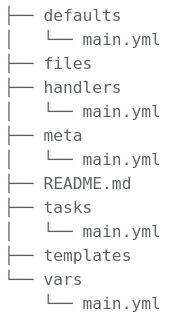
\includegraphics[width=3cm]{05_2018_Kharkevich6.png}
  %\caption{}
  \label{Kharkevich1}
\end{figure}

В рамках данной структуры и описываются все необходимые действия по приведению части системы в ожидаемое состояние.
После финализации данной роли можно осуществить публикацию её на GitHub с последующим импортом в ansible-galaxy. Но при такой упрощенной системе публикации нет никакого процесса контроля качества данной роли.

\subsection*{Соответствие стилевым рекомендациям}

Одним из самых простых механизмов проверки качества кода является использование статического анализатора кода. Наиболее эффективными инструментами для Ansible являются:

\begin{itemize}
  \item yamllint (\url{https://pypi.org/project/yamllint/})
  \item ansible-lint (\url{https://pypi.org/project/ansible-lint/})
\end{itemize}

Последний, в свою очередь, может использовать как встроенный, так и подключаемый список правил.
Кроме того, данные статические анализаторы могут быть встроены в различные системы непрерывной интеграции для предотвращения попадания кода, несоответствующего требованиям.

\subsection*{Платформа для тестирования}

Для тестирования Ansible ролей, на сегодняшний день, molecule является наиболее удобным инструментом. Который, в свою очередь поддерживает множественные интеграции с различными средами, которые могут выступать в роли целевых платформ; такие как: Docker, AWS, Microsoft Azure, Google Cloud Platform и др.
Интегрировать molecule-тесты можно в любой момент, выполнив инициализацию нового тестового сценария (molecule init scenario -r \textless{}имя\_роли\textgreater{}). После данной инициализации будет создана структура для тестов с параметрами по умолчанию (galaxy~--- для решения зависимостей, docker~--- как целевая платформа для разворачивания тестовой среды, default~--- как имя тестового сценария, testinfra~--- как тестовый фреймворк для проведения интеграционных тестов).
Типовая структура роли после инициализации тестового сценария molecule:
\newpage
\begin{figure}[h!]
  \centering
  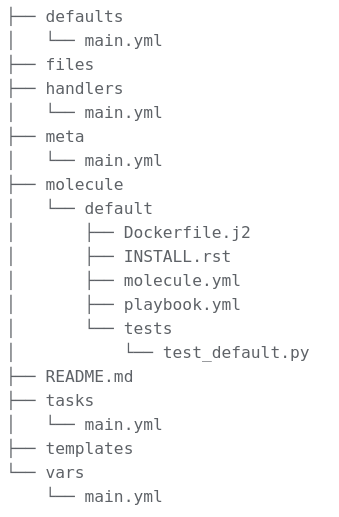
\includegraphics[width=5cm]{05_2018_Kharkevich5.png}
  %\caption{}
  \label{Kharkevich2}
\end{figure}


Без какого-либо дополнительного вмешательства, стразу после инициализации, данный тест готов проверить вашу роль на статический анализ, успешность применения в тестовой среде и идемпотентность.
Для поддержания качества разрабатываемой роли в требуемом состоянии необходимо подключить какую-либо из систем непрерывной интеграции.

\subsection*{Непрерывная интеграция (CI)}

Travis-CI является одной из самых доступных систем непрерывной интеграции для проектов с открытым исходным кодом. Для подключения данной системы достаточно просто разместить файл .travis.yml в корне репозитория и активировать CI на веб-сайте \url{https://travis-ci.org}

\begin{center}
\begin{figure}[h!]
  \centering
  
\includegraphics[width=5cm]{05_2018_Kharkevich1.png}
  %\caption{Блок-схема примерной системы распознавания РОГ}
  \label{Kharkevich3}
\end{figure}
\end{center} 
Содержимое .travis.yml файла для вышеописанной роли может быть следующем:

\begin{verbatim}
---
dist: xenial
sudo: required
language: python
python:
  - "2.7"
services:
  - docker
before_install:
  - git clone -b ${lint_version} https://github.com/
lean-delivery/ansible-lint-rules.git ~/ansible-lint-rules
install:
  - pip install --upgrade ansible==2.5.5 ansible-lint==3.4.21 
docker-py==1.10.6 molecule==2.13.1 pyOpenSSL PyYAML==3.12
  - ansible --version
  - molecule --version
script:
  - ansible-lint -c .ansible-lint `find . -regex ".*\.\(yml\)"`
  - molecule test
notifications:
  webhooks: https://galaxy.ansible.com/api/v1/notifications/\end{verbatim}
После активации CI при последующем изменении кода в репозитории запустится процесс тестирования в рамках вышеописанного molecule-сценария:

\begin{center}
\begin{figure}[h!]
  \centering
  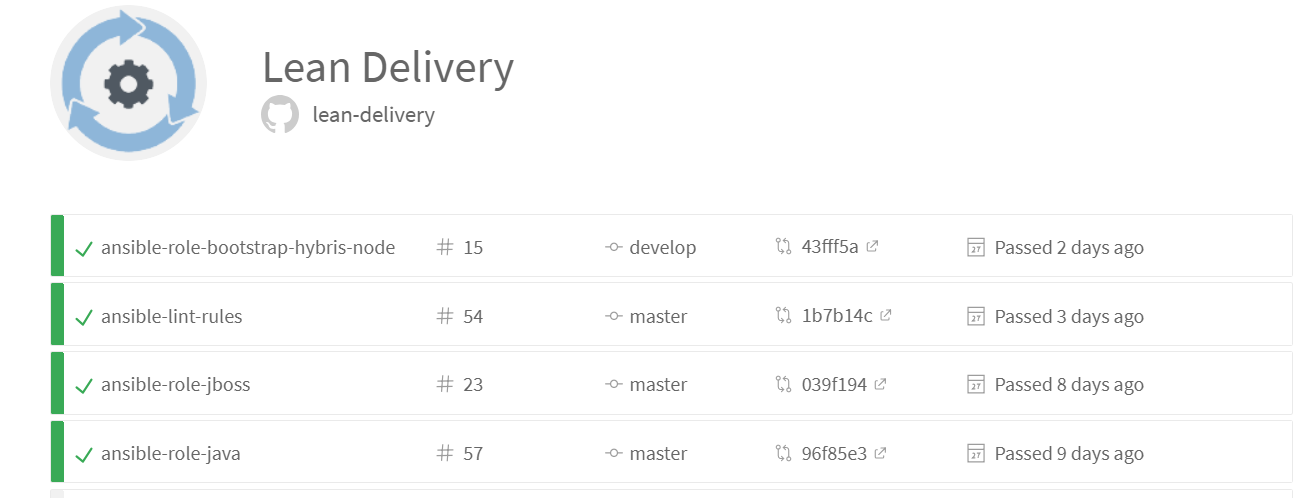
\includegraphics[width=9cm]{05_2018_Kharkevich2.png}
  %\caption{Блок-схема примерной системы распознавания РОГ}
  \label{Kharkevich4}
\end{figure}
\end{center} 

Иногда бывает необходимо проводить тестирование в непубличных средах. Например, вы хотите провести тестирование не только в докере, но и в других облачных сервисах, при этом вы хотите препятствовать утечке API ключа, который понадобится для запуска тестовых сред. В этом случае можно использовать немного более сложную топологию интеграции и подключить GitLab CI к GitHub репозиториям.
Для этого вам необходимо на веб-сайте \url{https://gitlab.com} подключить ваш GitHub репозиторий как “CI/CD for external repo”. После этого у вас появится зеркало вашего репозитория, цель которого лишь запускать ваш код на сборку и тестирование, руководствуясь инструкциями из файла .gitlab-ci.yml. В данном случае CI топология будет аналогична CI с использованием Travis-CI, за исключением возможности подключения GitLab Runner, который размещается в вашей приватной сети (возможность использовать публичные GitLab Runner остаётся). 

\begin{center}
\begin{figure}[h!]
  \centering
  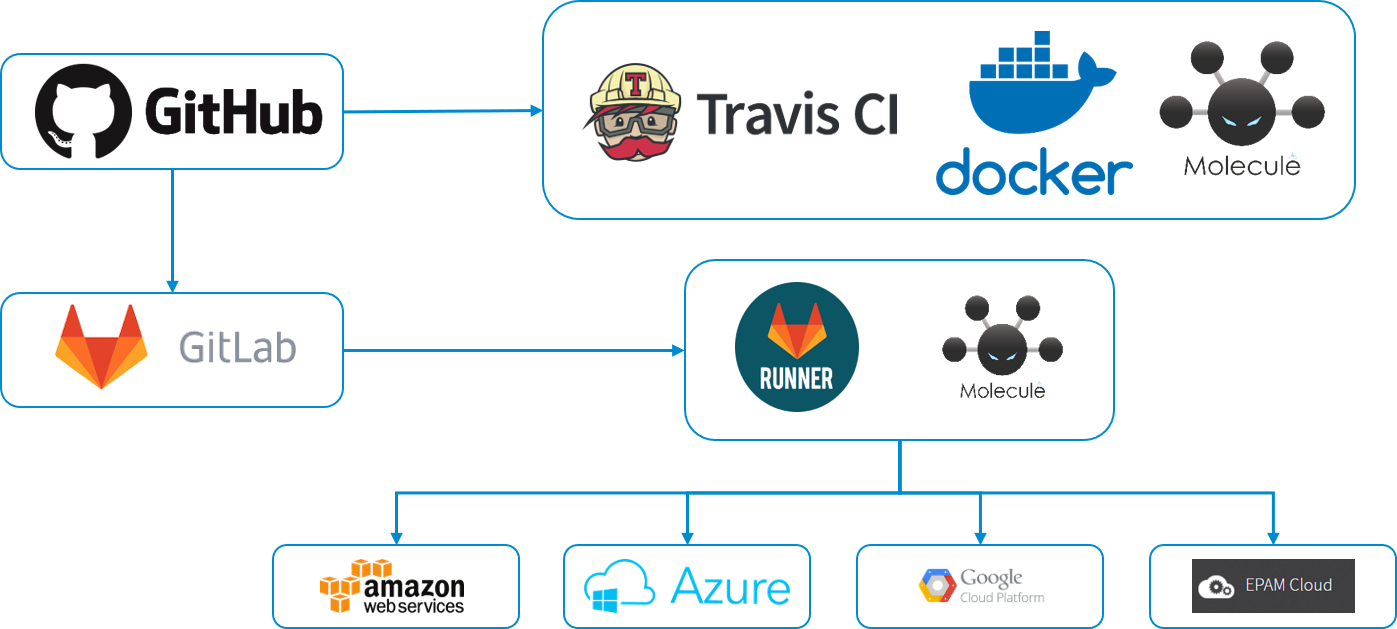
\includegraphics[width=5cm]{05_2018_Kharkevich3.png}
  %\caption{Блок-схема примерной системы распознавания РОГ}
  \label{Kharkevich5}
\end{figure}
\end{center} 

\subsection*{Вместо заключения}

\begin{center}
\begin{figure}[h!]
  \centering
  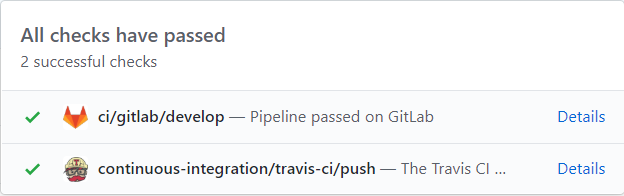
\includegraphics[width=9cm]{05_2018_Kharkevich4.png}
  %\caption{Блок-схема примерной системы распознавания РОГ}
  \label{Kharkevich6}
\end{figure}
\end{center} 

Интегрировав данные инструменты в рамках процесса тестирования Ansible ролей, мы получили достаточно простой, но тем не менее эффективный инструмент, позволяющий поддерживать нашу кодовую базу в единообразном состоянии и быть уверенными в том, что данные роли работоспособны на различных целевых платформах вне зависимости от (не)желания этому помешать.

\begin{thebibliography}{20}
  \bibitem{Kharkevich-1} Molecule \url{https://molecule.readthedocs.io}
  \bibitem{Kharkevich-2} Примеры Ansible ролей \url{https://galaxy.ansible.com/lean_delivery/}
  \bibitem{Kharkevich-3} Интеграция GitLab CI и GitHub \url{https://about.gitlab.com/features/github/}
  \bibitem{Kharkevich-4} Travis-CI \url{https://github.com/marketplace/travis-ci}
  \bibitem{Kharkevich-5} Дополнительные ansible-lint правила \url{https://github.com/lean-delivery/ansible-lint-rules}
\end{thebibliography}

\end{document}

\documentclass[10pt, a5paper]{article}
\usepackage{pdfpages}
\usepackage{parallel}
\usepackage[T2A]{fontenc}
\usepackage{ucs}
\usepackage[utf8x]{inputenc}
\usepackage[polish,english,russian]{babel}
\usepackage{hyperref}
\usepackage{rotating}
\usepackage[inner=2cm,top=1.8cm,outer=2cm,bottom=2.3cm,nohead]{geometry}
\usepackage{listings}
\usepackage{graphicx}
\usepackage{wrapfig}
\usepackage{longtable}
\usepackage{indentfirst}
\usepackage{array}
\newcolumntype{P}[1]{>{\raggedright\arraybackslash}p{#1}}
\frenchspacing
\usepackage{fixltx2e} %text sub- and superscripts
\usepackage{icomma} % коскі ў матэматычным рэжыме
\PreloadUnicodePage{4}

\newcommand{\longpage}{\enlargethispage{\baselineskip}}
\newcommand{\shortpage}{\enlargethispage{-\baselineskip}}

\def\switchlang#1{\expandafter\csname switchlang#1\endcsname}
\def\switchlangbe{
\let\saverefname=\refname%
\def\refname{Літаратура}%
\def\figurename{Іл.}%
}
\def\switchlangen{
\let\saverefname=\refname%
\def\refname{References}%
\def\figurename{Fig.}%
}
\def\switchlangru{
\let\saverefname=\refname%
\let\savefigurename=\figurename%
\def\refname{Литература}%
\def\figurename{Рис.}%
}

\hyphenation{admi-ni-stra-tive}
\hyphenation{ex-pe-ri-ence}
\hyphenation{fle-xi-bi-li-ty}
\hyphenation{Py-thon}
\hyphenation{ma-the-ma-ti-cal}
\hyphenation{re-ported}
\hyphenation{imp-le-menta-tions}
\hyphenation{pro-vides}
\hyphenation{en-gi-neering}
\hyphenation{com-pa-ti-bi-li-ty}
\hyphenation{im-pos-sible}
\hyphenation{desk-top}
\hyphenation{elec-tro-nic}
\hyphenation{com-pa-ny}
\hyphenation{de-ve-lop-ment}
\hyphenation{de-ve-loping}
\hyphenation{de-ve-lop}
\hyphenation{da-ta-ba-se}
\hyphenation{plat-forms}
\hyphenation{or-ga-ni-za-tion}
\hyphenation{pro-gramming}
\hyphenation{in-stru-ments}
\hyphenation{Li-nux}
\hyphenation{sour-ce}
\hyphenation{en-vi-ron-ment}
\hyphenation{Te-le-pathy}
\hyphenation{Li-nux-ov-ka}
\hyphenation{Open-BSD}
\hyphenation{Free-BSD}
\hyphenation{men-ti-on-ed}
\hyphenation{app-li-ca-tion}

\def\progref!#1!{\texttt{#1}}
\renewcommand{\arraystretch}{2} %Іначай формулы ў матрыцы зліпаюцца з лініямі
\usepackage{array}

\def\interview #1 (#2), #3, #4, #5\par{

\section[#1, #3, #4]{#1 -- #3, #4}
\def\qname{LVEE}
\def\aname{#1}
\def\q ##1\par{{\noindent \bf \qname: ##1 }\par}
\def\a{{\noindent \bf \aname: } \def\qname{L}\def\aname{#2}}
}

\def\interview* #1 (#2), #3, #4, #5\par{

\section*{#1\\{\small\rm #3, #4. #5}}

\def\qname{LVEE}
\def\aname{#1}
\def\q ##1\par{{\noindent \bf \qname: ##1 }\par}
\def\a{{\noindent \bf \aname: } \def\qname{L}\def\aname{#2}}
}

\begin{document}
\title{Консольно-ориентированные сервисы: wttr.in, cheat.sh, rate.sx~--- Идея, использвание, создание\footnote{\url{igor@chub.in}, \url{https://lvee.org/en/abstracts/278}}}
\author{Игорь Чубин (Igor Chubin)}
\maketitle
\begin{abstract}
Console orineted services: wttr.in, cheat.sh, rate.sx: idea, usage, and creation. 
The presentation is devoted to console oriented services, such as: wttr.in, cheat.sh, rate.sx. Which popular console oriented services exist currently and how can they be used in everyday life; what advantages and disadvantages do they have; how services like that could be created.
\end{abstract}


\subsubsection*{Консольно-ориентированные сервисы}

На рубеже 2015 и 2016 годов, в дополнение к традиционно существующим типам
программ и служб, доступным пользователям UNIX/Linux, а именно локально инсталлируеммым программам, доступным для использования в консоли или в графической оболочке, и, программам, работающим на внешних серверах, и доступным через web-интерфейс, появился третий, новый, тип программ, совмещающих в себе свойства первых двух типов: так называемые консольно-ориентированные сервисы, которые не требуют инсталляции и доступны к использованию как из терминала, так и из браузера.

Благодаря своей простоте использования, полному отсутствию необходимости
инсталляции и конфигурирования и ряду других преимуществ, они начали быстро завоёвывать популярность среди пользователей
консоли UNIX/Linux систем.

Характерной особенностью таких сервисов является то, что их использование, с точки зрения пользователя, напоминает использование обыкновенного простого веб-сайта, но только в отличие от веб-сайта, для них наличие браузера
не обязательно, вместо него можно использовать простые HTTP-клиенты,
такие как curl, httpie или wget. Путешествие по гиперссылкам при этом
заменяется манипуляциями с URL, который в случае консольных сервисов,
как правило, чрезвычайно прост и интуитивно понятен.

Важным аспектом сервисов является и то, что они построены таким образом,
что отображаются в консоли UNIX/Linux системы и в браузере одинаково.
Это достигается при помощи анализа заголовка User-Agent запроса,
в зависимости от которого ответ генерируется в форме HTML, пригодной для браузера, или в ANSI, пригодной для терминала. Такой подход существенно облегчает новым пользователям порог вхождения и начало использования консольных сервисов.

Следующие команды, выполненные в терминале, позволют получить первое впечатление о том, что такое консольные сервисы, и как они выглядят с точки зрения пользователя:

\ldots

    curl be.wttr.in/Minsk

    curl rate.sx/btc

    curl cheat.sh/lua/copy+file

\ldots

Если использовать эти же строки запроса в браузере, то можно увидеть ответы
аналогичные тем, что получены при запросе из терминала.

Как уже было сказано, сервисы созданные в соответствии с этим таким подходом
обладают множеством преимуществ как в сравнении с сервисами, созданными для использования из Web-браузера, так и в сравнении с традиционными консольными приложениями:

\begin{itemize}
  \item скорость;
  \item совместимость;
  \item очень низкие требования к клиенту;
  \item прекрасная возможность интеграции;
  \item простота и краткость;
  \item анонимность использования;
  \item и так далее.
\end{itemize}

В рамках популяризации идеи создания консольных сервисов, было создано
несколько типичных консольных сервисов, некоторые из которых получили большую
известность, и сейчас уже знакомы большому числу активных пользователей консоли UNIX/Linux во всём мире. Некоторые из них описаны ниже.

Кроме того, был создан специальный фреймворк, curlator, который существенно
упрощает создание консольных сервисов, и делает задачу создания консольных
сервисов доступным любому пользователю UNIX/Linux-систем, не требуя от него
никаких специальных знаний. Создание сервиса при этом по сложности соизмеримо с инсталляцией и начальным конфигурированием обычной UNIX/Linux-программы.

\subsubsection*{Примеры популярных консольно-ориентированных сервисов}

\paragraph{wttr.in}

wttr.in~--- сервис прогноза погоды, позволяет получить информацию о погоде в любой точке земного шара на одном из более 50 мировых языков; как и любой консольный сервис не требует никакой инсталляции и конфигурирования.

Примеры использования:

\ldots

    curl wttr.in

    curl ru.wttr.in

    curl be.wttr.in/Minsk

    curl uk.wttr.in/Москва

\ldots

\paragraph{cheat.sh}

cheat.sh~--- сервис подсказок по UNIX/Linux-командам и языкам программирования.

С его помощью можно получить подсказку с наиболее популярными примерами 
использования основных программ UNIX/Linux (сейчас сервис покрывает более 1000 команд), а так же получить ответы на практически любой вопрос по практически любому языку программирования.

Примеры использования:

\ldots

    curl cheat.sh

    curl cheat.sh/btrfs

    curl cheat.sh/az\~{}snapshot

    curl cheat.sh/lua/copy+file

    curl cheat.sh/ruby/скопировать+файл

    curl cheat.sh/python/створити+дерево+каталогів

\ldots

\paragraph{rate.sx}

rate.sx~--- сервис отслеживания обменных курсов валюты и криптовалюты.

С его помощью можно получить информацию о текущей и исторической стоимости
любой (из 500 наиболее популярных) криптовалюты на рынке, а так же её рыночную капитализацию, объём торгов и множество других характеристик.

\ldots

    curl rate.sx

    curl rate.sx/btc

    curl rate.sx/btc@1w

    curl rate.sx/btc/eth@1w

    curl eur.rate.sx/btc

\ldots

\paragraph{Другие сервисы}

Существует ряд других, менее популярных консольных сервисов, популярность которых, однако, растёт. Актуальный список сервисов доступен по адресу:  \url{https://github.com/chubin/awesome-console-services}

\subsubsection*{Об авторе}

Игорь Чубин~--- разработчик программного обеспечения, активный убеждённый пользователь и энтузиаст программного обеспечения. Основная его работа на протяжении последних десяти лет, это разработка высокопроизводительной распределённой реляционной базы данных Exasol.

В свободное от работы время он занимается разработкой и продвижением консольно-ориентированных сервисов.

Github: \url{https://github.com/chubin}

Twitter: \url{https://twitter.com/igor\_chubin}

StackOverflow: \url{https://stackoverflow.com/users/1458569/}

\end{document}

\documentclass[10pt, a5paper]{article}
\usepackage{pdfpages}
\usepackage{parallel}
\usepackage[T2A]{fontenc}
\usepackage{ucs}
\usepackage[utf8x]{inputenc}
\usepackage[polish,english,russian]{babel}
\usepackage{hyperref}
\usepackage{rotating}
\usepackage[inner=2cm,top=1.8cm,outer=2cm,bottom=2.3cm,nohead]{geometry}
\usepackage{listings}
\usepackage{graphicx}
\usepackage{wrapfig}
\usepackage{longtable}
\usepackage{indentfirst}
\usepackage{array}
\newcolumntype{P}[1]{>{\raggedright\arraybackslash}p{#1}}
\frenchspacing
\usepackage{fixltx2e} %text sub- and superscripts
\usepackage{icomma} % коскі ў матэматычным рэжыме
\PreloadUnicodePage{4}

\newcommand{\longpage}{\enlargethispage{\baselineskip}}
\newcommand{\shortpage}{\enlargethispage{-\baselineskip}}

\def\switchlang#1{\expandafter\csname switchlang#1\endcsname}
\def\switchlangbe{
\let\saverefname=\refname%
\def\refname{Літаратура}%
\def\figurename{Іл.}%
}
\def\switchlangen{
\let\saverefname=\refname%
\def\refname{References}%
\def\figurename{Fig.}%
}
\def\switchlangru{
\let\saverefname=\refname%
\let\savefigurename=\figurename%
\def\refname{Литература}%
\def\figurename{Рис.}%
}

\hyphenation{admi-ni-stra-tive}
\hyphenation{ex-pe-ri-ence}
\hyphenation{fle-xi-bi-li-ty}
\hyphenation{Py-thon}
\hyphenation{ma-the-ma-ti-cal}
\hyphenation{re-ported}
\hyphenation{imp-le-menta-tions}
\hyphenation{pro-vides}
\hyphenation{en-gi-neering}
\hyphenation{com-pa-ti-bi-li-ty}
\hyphenation{im-pos-sible}
\hyphenation{desk-top}
\hyphenation{elec-tro-nic}
\hyphenation{com-pa-ny}
\hyphenation{de-ve-lop-ment}
\hyphenation{de-ve-loping}
\hyphenation{de-ve-lop}
\hyphenation{da-ta-ba-se}
\hyphenation{plat-forms}
\hyphenation{or-ga-ni-za-tion}
\hyphenation{pro-gramming}
\hyphenation{in-stru-ments}
\hyphenation{Li-nux}
\hyphenation{sour-ce}
\hyphenation{en-vi-ron-ment}
\hyphenation{Te-le-pathy}
\hyphenation{Li-nux-ov-ka}
\hyphenation{Open-BSD}
\hyphenation{Free-BSD}
\hyphenation{men-ti-on-ed}
\hyphenation{app-li-ca-tion}

\def\progref!#1!{\texttt{#1}}
\renewcommand{\arraystretch}{2} %Іначай формулы ў матрыцы зліпаюцца з лініямі
\usepackage{array}

\def\interview #1 (#2), #3, #4, #5\par{

\section[#1, #3, #4]{#1 -- #3, #4}
\def\qname{LVEE}
\def\aname{#1}
\def\q ##1\par{{\noindent \bf \qname: ##1 }\par}
\def\a{{\noindent \bf \aname: } \def\qname{L}\def\aname{#2}}
}

\def\interview* #1 (#2), #3, #4, #5\par{

\section*{#1\\{\small\rm #3, #4. #5}}

\def\qname{LVEE}
\def\aname{#1}
\def\q ##1\par{{\noindent \bf \qname: ##1 }\par}
\def\a{{\noindent \bf \aname: } \def\qname{L}\def\aname{#2}}
}

\begin{document}
\title{Как поссорились Иван Интелович с Иваном Опёнковичем\footnote{\url{zhuk@openbsd.org}, \url{https://lvee.org/en/abstracts/281}}}
\author{Vadim Zhukov, Moscow, Russian Federation}
\maketitle
\begin{abstract}
This is the story about latest Intel tries to discriminate OpenBSD on getting pre-public disclosure infromation about vulnerabilities in its products.
\end{abstract}
Многие слышали историю о том, как OpenBSD «отлучили» от информации об уязвимостях Meltdown и Spectre.

В середине 2017 года Мэти Ванхоф (Mathy Vanhoef), молодой и при этом уже известный в определённых кругах специалист в области безопасности, уже несколько лет занимавшийся вопросами защиты беспроводных сетей IEEE 802.11 (Wi-Fi), последовательно обнаруживает ряд проблем в реализации протоколов WPA и WPA2, разной степени серьёзности. Самая крупная из проблем позднее получит персональное имя~--- KRACK.

Будучи добропорядочным исследователем, Ванхоф извещает разработчиков реализаций WPA о найденных проблемах с тем, чтобы каждый смог подготовить исправления. В том числе, 15 июля 2017 года такое извещение было отправлено приватно разработчикам OpenBSD. Выработанное решение было согласовано с Ванхофом и 30 августа, по согласованию с ним же, внесено в кодовую базу OpenBSD под видом минорного исправления. Подобная политика позволяет выступать open source-проектам на равных с разработчиками пропиетарных ОС, которые могут не боясь огласки выпускать обновления безопасности.

Тем не менее, несмотря на все предпринятые меры, данный коммит привлёк внимание специалистов по безопасности, исходная проблема была выявлена и раскрытие сведений об уязвимости пришлось провести безотлагательно. Поскольку переписка задействованных разработчиков OpenBSD с Ванхофом, по понятным причинам, не была публичной, то в широких кругах сложилось впечатление, что проект OpenBSD самовольно нарушил эмбарго на разглашение сведений об уязвимости.

В это же время ряд исследователей обнаружил уязвимость в микропроцессорах Intel, позволявшую медленно, но верно получать по косвенному каналу содержимое произвольных участков адресного пространства текущего процесса (включая содержимое ядра операционной системы). К делу подключились специалисты Intel а позднее, когда стала очевидна универсальность подхода, и других производителей микропроцессоров. Когда стало понятно, что данную уязвимость невозможно закрыть одним только изменением микрокода, к работе стали подключать разработчиков операционных систем. Однако в свете упомянутых выше событий, связанных с KRACK, компания Intel (и, возможно, другие заинтересованные лица) настояла на невключении проекта OpenBSD как неблагонадёжного партнёра.

Изначально эмбарго планировалось снять в середине января, однако допущенная в LKML утечка вынудила сдвинуть сроки. Фактически, повторилась описанная выше ситуация, но теперь уже с Linux: журналисты из The Register (и не только они) обратили внимание на поток серьёзных патчей, в результате чего анонс был срочно перенесён на 4-е января. Именно тогда разработчики OpenBSD (как и DragonFly BSD? Кто ещё? \% ) узнали о проблеме~--- наравне с широкой общественностью. Из-за крайне высокой сложности проблемы работа над исправлением ситуации заняла не один месяц. В ходе работы по конструированию обходных путей для Meltdown/Spectre были решены следующие задачи:

\begin{itemize}
  \item разделение адресных пространств ядра и приложения;
  \item модификация компиляторов для генерации защищающего от Meltdown/Specre кода;
  \item реализация инфраструктуры обновления микрокода ЦП Intel.
\end{itemize}

Однако на этом дело не закончилось: с каждым месяцем исследователи находили всё новые уязвимости в ЦП. И далеко не все из них разделяли мнение о том, что OpenBSD надо «наказать». Например, Бен Грас (Ben Gras) из VUSec по собственной воле поделился с разработчиками OpenBSD подробностями найденной им уязвимости TLBleed, позволяющей организовать утечку секретных ключей за счёт эксплуатации особенностей Intel Hyper Threading (на процессорах с одновременной многопоточностью других производителей организовать эффективную атаку оказалось затруднительно). Ещё более интересная ситуация сложилась с уязвимостью LazyFP: до разработчиков OpenBSD дошли слухи о наличии уязвимости, связанной с сохранением состояния сопроцессора. По этим скудным обрывкам был создан и закоммичен патч, о котором Тео де Раадт, лидер проекта, рассказал на конференции BSDCan. Через пять часов после этого Колин Персиваль, бывший FreeBSD security officer, смог создать рабочий эксплоит~--- в результате проект OpenBSD, не нарушив эмбарго, таки поспособствовал досрочному анонсу уязвимости (полностью подробности на момент написания этих строк по-прежнему не раскрыты).

Таким образом можно констатировать, что изоляция проекта OpenBSD не удалась, и следует ожидать изменения позиции Intel (и других производителей, разделявших отношение Intel к OpenBSD) по вопросам предварительного информирования об уязвимости.

\end{document}

\documentclass[10pt, a5paper]{article}
\usepackage{pdfpages}
\usepackage{parallel}
\usepackage[T2A]{fontenc}
\usepackage{ucs}
\usepackage[utf8x]{inputenc}
\usepackage[polish,english,russian]{babel}
\usepackage{hyperref}
\usepackage{rotating}
\usepackage[inner=2cm,top=1.8cm,outer=2cm,bottom=2.3cm,nohead]{geometry}
\usepackage{listings}
\usepackage{graphicx}
\usepackage{wrapfig}
\usepackage{longtable}
\usepackage{indentfirst}
\usepackage{array}
\newcolumntype{P}[1]{>{\raggedright\arraybackslash}p{#1}}
\frenchspacing
\usepackage{fixltx2e} %text sub- and superscripts
\usepackage{icomma} % коскі ў матэматычным рэжыме
\PreloadUnicodePage{4}

\newcommand{\longpage}{\enlargethispage{\baselineskip}}
\newcommand{\shortpage}{\enlargethispage{-\baselineskip}}

\def\switchlang#1{\expandafter\csname switchlang#1\endcsname}
\def\switchlangbe{
\let\saverefname=\refname%
\def\refname{Літаратура}%
\def\figurename{Іл.}%
}
\def\switchlangen{
\let\saverefname=\refname%
\def\refname{References}%
\def\figurename{Fig.}%
}
\def\switchlangru{
\let\saverefname=\refname%
\let\savefigurename=\figurename%
\def\refname{Литература}%
\def\figurename{Рис.}%
}

\hyphenation{admi-ni-stra-tive}
\hyphenation{ex-pe-ri-ence}
\hyphenation{fle-xi-bi-li-ty}
\hyphenation{Py-thon}
\hyphenation{ma-the-ma-ti-cal}
\hyphenation{re-ported}
\hyphenation{imp-le-menta-tions}
\hyphenation{pro-vides}
\hyphenation{en-gi-neering}
\hyphenation{com-pa-ti-bi-li-ty}
\hyphenation{im-pos-sible}
\hyphenation{desk-top}
\hyphenation{elec-tro-nic}
\hyphenation{com-pa-ny}
\hyphenation{de-ve-lop-ment}
\hyphenation{de-ve-loping}
\hyphenation{de-ve-lop}
\hyphenation{da-ta-ba-se}
\hyphenation{plat-forms}
\hyphenation{or-ga-ni-za-tion}
\hyphenation{pro-gramming}
\hyphenation{in-stru-ments}
\hyphenation{Li-nux}
\hyphenation{sour-ce}
\hyphenation{en-vi-ron-ment}
\hyphenation{Te-le-pathy}
\hyphenation{Li-nux-ov-ka}
\hyphenation{Open-BSD}
\hyphenation{Free-BSD}
\hyphenation{men-ti-on-ed}
\hyphenation{app-li-ca-tion}

\def\progref!#1!{\texttt{#1}}
\renewcommand{\arraystretch}{2} %Іначай формулы ў матрыцы зліпаюцца з лініямі
\usepackage{array}

\def\interview #1 (#2), #3, #4, #5\par{

\section[#1, #3, #4]{#1 -- #3, #4}
\def\qname{LVEE}
\def\aname{#1}
\def\q ##1\par{{\noindent \bf \qname: ##1 }\par}
\def\a{{\noindent \bf \aname: } \def\qname{L}\def\aname{#2}}
}

\def\interview* #1 (#2), #3, #4, #5\par{

\section*{#1\\{\small\rm #3, #4. #5}}

\def\qname{LVEE}
\def\aname{#1}
\def\q ##1\par{{\noindent \bf \qname: ##1 }\par}
\def\a{{\noindent \bf \aname: } \def\qname{L}\def\aname{#2}}
}

\begin{document}
\title{Между <<до>> и <<ля>>: какие прелести сохранил Си в современном мире?\footnote{\url{zhuk@openbsd.org}, \url{https://lvee.org/en/abstracts/282}}}
\author{Vadim Zhukov, Moscow, Russian Federation}
\maketitle
\begin{abstract}
An overview of applicability of C language in modern world, demonstrating its weak and strong sides.
\end{abstract}
C появился в 1969 году, и на тот момент считался высокоуровневым языком программирования. В настоящее же время существует огромное количество языков программирования, куда более удобных, предсказуемых и весьма производительных. Что же позволяет данному языку <<https://tproger.ru/articles/github-top-10-languages-2017/(оставаться востребованным)>>? И насколько сложным в действительности является программирование на современном С?~--- на эти вопросы мы и будем отвечать. Здесь не будет подробного разбора отличий от C++ и других без лишних усилий доступных вещей.

Язык программирования не мог бы оставаться столько лет актуальным без развития. И язык действительно развивается, в данное время~--- вначале под эгидой ANSI, а сейчас, как и C++ (но другой рабочей группой), под эгидой ISO.

Некоторые примеры полезной эволюции языка\footnote{\url{https://en.cppreference.com/w/c/language/history}}:

\begin{itemize}
  \item имена аргументов в объявлениях функций
  \item типы void и void*
  \item типы size\_t, ptrdiff\_t, (u)intN\_t и т.д.
  \item объявление переменных посреди кода
  \item выкидывание изначально некорректных концепций, например, gets()
  \item безымянные struct и union
  \item поддержка Unicode
  \item поддержка многопоточности
\end{itemize}

Не очень удачные решения:

\begin{itemize}
  \item strict aliasing
  \item \emph{Exit() и quick}exit()
\end{itemize}

Откровенно слабые стороны C:

\begin{itemize}
  \item rand()+srand()
  \item недостаточный контроль обращений к памяти в динамических буферах
\end{itemize}

Странности языка C с точки зрения прикладного программиста:

\begin{itemize}
  \item беззнаковые целочисленные типы~--- необходимы для работы с памятью (как иначе обратиться к адресу $0\times8000$ на 16-битной системе?).
\end{itemize}

\begin{itemize}
  \item отсутствие реализаций <<из коробки>> типовых структур таких как словари и деревья~--- разные решения могут давать принципиально разную производительность и задавать разные требования (например: служебные поля списка/дерева хранятся в самих структурах или за их пределами?), стандартными попросту мало кто будет пользоваться.
\end{itemize}

\begin{itemize}
  \item нет наследования~--- в системном программировании оно нужно только для данных, поэтому гарантированное «первый член структуры находится по тому же адресу, что и структура» перевешивает плюсы виртуальных вызовов (без которых о наследовании говорить не приходится в принципе).
\end{itemize}

Мифы и правда о современном C:

\begin{itemize}
  \item C пригоден для написания прикладных приложений~--- миф. Если только не считать прикладным приложением RTSP-\linebreak сервер для бюджетного одноплатника.
\end{itemize}

\begin{itemize}
  \item Используя указатели, легко ошибиться~--- с указателями можно, действительно, делать что угодно, но современные компиляторы предупредят в большинстве случаев. Тем не менее, действительно, самые частые ошибки~--- выход за пределы массива и использование освобождённой памяти~--- связаны именно с использованием указателей.
\end{itemize}

\begin{itemize}
  \item goto, это же очень плохо?~--- нет, это, как минимум, альтернатива обработке исключений, пример будет дальше.
\end{itemize}

\begin{itemize}
  \item В нём есть void*, и это ужасно~--- в других языках изобретают костыли вроде Object, ровно для того же самого, так что не ужаснее прочих. Что же касается риска получить из void* не то, что ожидается, то он сильно переоценён, на практике никто не кладёт в одном и том же коде в одно и то же void*-поле указатели на несовместимые структуры.
\end{itemize}

\begin{itemize}
  \item В C нельзя скрыть детали реализации~--- можно, и это повсеместно используется: достаточно объявить (но не определить) структуру и далее пользоваться указателями на неё.
\end{itemize}

\begin{itemize}
  \item Нужно постоянно следить за освобождением памяти~--- за памятью нужно следить везде. Забытая ссылка в языке с подсчётом ссылок на объекты точно так же заставит память утечь, garbage collector тоже никаких гарантий не даст. Использование же простейших, не зависящих от языка, правил позволяет значительно минимизировать количество утечек. Вот найти источник утечки~--- это в C сложнее, чем в Java, да~--- средства вроде valgrind работают не везде и не всегда.
\end{itemize}

\begin{itemize}
  \item В C нельзя складывать строки~--- синтаксиса специального нет, есть чересчур опасная strcat(); есть более вменяемые\linebreak strlcat() и asprintf(), но они вне стандарта языка.
\end{itemize}

\begin{itemize}
  \item C полностью перекрывается C++~--- помимо того, что есть вещи, которые можно делать в C, нельзя в C++, как то: приравнивать (без явного приведения типов) void* к другим указателям, многосимвольные константные литералы, restrict и так далее,~--- есть и целый ряд не совместимых решений, например, inline-функции.
\end{itemize}

\begin{itemize}
  \item Макросы суть зло~--- как и почти всё остальное в Си, они позволяют прострелить себе и окружающим ноги самыми разными способами, но есть best practicies, от этого спасающие, пример ниже.
\end{itemize}

\begin{itemize}
  \item C это сплошные переполнения буфера~--- современные компиляторы давным-давно умеют как добавлять средства детектирования таких ситуаций, так и предупреждать о заведомо опасных конструкциях, поэтому подавляющее большинство проблем этого класса отлавливаются в ходе разработки. Средства детектирования можно обойти, конечно, но для этого требуется найти особую утечку данных, впрочем, это уже отдельный разговор.
\end{itemize}

\begin{itemize}
  \item C не нужен, когда есть Rust,~--- написать компилятор ANSI C может практически любой вменяемый студент технического ВУЗа, а вот с Rust всё сложнее. Пока есть заметная потребность в написании компиляторов (или хотя бы бэкендов) для новых платформ, C будет выигрывать у Rust, по крайней мере, в ближайшие лет пять (срок получения высшего образования) точно.
\end{itemize}

Примеры изящных решений, специфичных для C:

1. Код с обработкой ошибок и goto:

\begin{verbatim}
int
open_server_socket(const struct srvconf *conf) {
    int sock;

    if ((sock = socket(conf->af, SOCK_DGRAM|SOCK_CLOEXEC,
	 0)) == -1)
        return -1;
    if (setsockopt(sock, SOL_SOCKET, SO_RCVBUF, conf->
	rcvsize, sizeof(conf->rcvsize)) == -1)
        goto fail;
    if (conf->rtable >= 0) {
        if (setsockopt(sock, SOL_SOCKET, SO_RTABLE, 
	    conf->rtable, sizeof(conf->rtable)) == -1)
            goto fail;
    }
    if (setsockopt(sock, SOL_SOCKET, SO_SNDBUF, conf->
	rcvsize, sizeof(conf->rcvsize)) == -1)
        goto fail;
    if (bind(sock, (const struct sockaddr *)conf->addr,
	conf->addrlen) == -1)
        goto fail;
    if (listen(sock, conf->connqlen) == -1)
        goto fail;
    return sock;

fail:
    warn("%s", __func__);
    close(sock);
    return -1;
}\end{verbatim}
2. Эффективный (деструктивный) разбор строки без выделения памяти:

\begin{verbatim}
// RFC 3264
// m=video 29034 RTP/AVP 96
// a=rtpmap:96 H.264/90000

struct sdp_line {
    char     op;
    char    *name;  // не-NULL для атрибутов
    char    *value;
};

int
sdp_parse_line(char *line, struct sdp_line *sdpl) {
    char    *colon;

    if (line[0] == '\0' || line[1] != '=')
        goto inval;
    sdpl->op = line[0];
    line += 2;
    if (sdpl->op == 'a') {
        if ((colon = strchr(line, ':')) == NULL || 
	     colon == line)
            goto inval;
        *colon = '\0';
        sdpl->name = line;
        sdpl->value = colon + 1;
    } else {
        sdpl->name = NULL;
        sdpl->value = line;
    }
    return 0;

inval:
	errno = EINVAL;
	return -1;
}\end{verbatim}
3. Пример макросов, предназначенных для работы с передаваемыми по IPC сообщениями, из реального кода:

\begin{verbatim}
#define imsg_get_plain(p, left, v) \
	do { \
		if ((left) < sizeof((v))) \
			fatalx("%s: short imsg read
 			of %s", __func__, #v); \
		memcpy(&(v), (p), sizeof((v))); \
		(p) += sizeof((v)); \
		(left) -= sizeof((v)); \
	} while(0)

#define imsg_put_plain(p, left, v) \
	do { \
		if ((left) < sizeof((v))) \
			fatalx("%s: short imsg write 
			    of %s", __func__, #v); \
		memcpy((p), &(v), sizeof((v))); \
		(p) += sizeof((v)); \
		(left) -= sizeof((v)); \
	} while(0)

// примеры использования:
imsg_put_plain(buf, buflen, frag->fr_id);
imsg_put_plain(buf, buflen, frag->fr_from);
imsg_put_plain(buf, buflen, frag->fr_till);
imsg_put_plain(buf, buflen, frag->fr_nframes);
imsg_put_plain(buf, buflen, frag->fr_size);
// ...
imsg_get_plain(buf, buflen, frag->fr_id);
imsg_get_plain(buf, buflen, frag->fr_from);
imsg_get_plain(buf, buflen, frag->fr_till);
imsg_get_plain(buf, buflen, frag->fr_nframes);
imsg_get_plain(buf, buflen, frag->fr_size);
\end{verbatim}
\end{document}

\documentclass[10pt, a5paper]{article}
\usepackage{pdfpages}
\usepackage{parallel}
\usepackage[T2A]{fontenc}
\usepackage{ucs}
\usepackage[utf8x]{inputenc}
\usepackage[polish,english,russian]{babel}
\usepackage{hyperref}
\usepackage{rotating}
\usepackage[inner=2cm,top=1.8cm,outer=2cm,bottom=2.3cm,nohead]{geometry}
\usepackage{listings}
\usepackage{graphicx}
\usepackage{wrapfig}
\usepackage{longtable}
\usepackage{indentfirst}
\usepackage{array}
\newcolumntype{P}[1]{>{\raggedright\arraybackslash}p{#1}}
\frenchspacing
\usepackage{fixltx2e} %text sub- and superscripts
\usepackage{icomma} % коскі ў матэматычным рэжыме
\PreloadUnicodePage{4}

\newcommand{\longpage}{\enlargethispage{\baselineskip}}
\newcommand{\shortpage}{\enlargethispage{-\baselineskip}}

\def\switchlang#1{\expandafter\csname switchlang#1\endcsname}
\def\switchlangbe{
\let\saverefname=\refname%
\def\refname{Літаратура}%
\def\figurename{Іл.}%
}
\def\switchlangen{
\let\saverefname=\refname%
\def\refname{References}%
\def\figurename{Fig.}%
}
\def\switchlangru{
\let\saverefname=\refname%
\let\savefigurename=\figurename%
\def\refname{Литература}%
\def\figurename{Рис.}%
}

\hyphenation{admi-ni-stra-tive}
\hyphenation{ex-pe-ri-ence}
\hyphenation{fle-xi-bi-li-ty}
\hyphenation{Py-thon}
\hyphenation{ma-the-ma-ti-cal}
\hyphenation{re-ported}
\hyphenation{imp-le-menta-tions}
\hyphenation{pro-vides}
\hyphenation{en-gi-neering}
\hyphenation{com-pa-ti-bi-li-ty}
\hyphenation{im-pos-sible}
\hyphenation{desk-top}
\hyphenation{elec-tro-nic}
\hyphenation{com-pa-ny}
\hyphenation{de-ve-lop-ment}
\hyphenation{de-ve-loping}
\hyphenation{de-ve-lop}
\hyphenation{da-ta-ba-se}
\hyphenation{plat-forms}
\hyphenation{or-ga-ni-za-tion}
\hyphenation{pro-gramming}
\hyphenation{in-stru-ments}
\hyphenation{Li-nux}
\hyphenation{sour-ce}
\hyphenation{en-vi-ron-ment}
\hyphenation{Te-le-pathy}
\hyphenation{Li-nux-ov-ka}
\hyphenation{Open-BSD}
\hyphenation{Free-BSD}
\hyphenation{men-ti-on-ed}
\hyphenation{app-li-ca-tion}

\def\progref!#1!{\texttt{#1}}
\renewcommand{\arraystretch}{2} %Іначай формулы ў матрыцы зліпаюцца з лініямі
\usepackage{array}

\def\interview #1 (#2), #3, #4, #5\par{

\section[#1, #3, #4]{#1 -- #3, #4}
\def\qname{LVEE}
\def\aname{#1}
\def\q ##1\par{{\noindent \bf \qname: ##1 }\par}
\def\a{{\noindent \bf \aname: } \def\qname{L}\def\aname{#2}}
}

\def\interview* #1 (#2), #3, #4, #5\par{

\section*{#1\\{\small\rm #3, #4. #5}}

\def\qname{LVEE}
\def\aname{#1}
\def\q ##1\par{{\noindent \bf \qname: ##1 }\par}
\def\a{{\noindent \bf \aname: } \def\qname{L}\def\aname{#2}}
}

\switchlang{en}
\begin{document}
\title{Licenses as a software\footnote{\url{bircoph@gmail.com}, \url {https://lvee.org/ru/abstracts/283}}}
\author{Andrew Savchenko, Moscow, Russian Federation}
\maketitle
\begin{abstract}
Free software licenses may be seen as software themselves: they are set of rules and algorithms of how to use software. As any software licenses are not perfect and have vulnerabilities which are exploited to limit our freedom. This talk is about how it happens and what mitigations are available.
\end{abstract}
As software licenses become more and more complex, one can see them as a software themselves as they define set of rules and algorithms of how to use software. Of course this statement applies for both\linebreak commercial and FLOSS (free/libre/open source software) licenses,\linebreak however this work will be focused on FLOSS ones only.

Like any software licenses are not perfect, they have design flaws and vulnerabilities, because it is impossible to account for all non-trivial cases and tiny details during license development.

One good example of such problem and its solution is Tivoisation issue~\cite{Savchenko-1}. GPLv2 has a vulnerability allowing manufacturers to block on hardware level user's freedom to update software, while keeping it for themselves, e.g. when hardware allows to run only manufacturer-signed software effectively blocking user from the freedom of using modified software. Formally such behaviour does not violate GPLv2.

So GPLv3 was created to address this and some other issues. But what is the price paid? GPLv2 is 340 lines, GPLv3 is 676 lines. We have more code to handle corner cases properly, but it is harder to understand it for common people. Complexity is the price and some users are repelled by it.

Some of open issues we are facing now:

\begin{itemize}
  \item Obfuscated patches, e.g. RedHat kernel patches shipped in already applied form~\cite{Savchenko-2}. Since they contain hundreds of in- and\linebreak interdependent changes; while formally in compliance with GPLv2, such distribution limits user's freedom to reuse modifications made.
  \item ZFS issue~\cite{Savchenko-3}: forcing redistribution and use of incompatible\\ binaries (CDDL and GPLv2). A corner case where corporations try to loose copyleft restrictions and many users support it because they want cool features and don't care much about licenses. The legal problem here is in what ``derivative/combined work'' means. Because the lack of clear definition, unfair entities try to violate GPLv2 by staying in formal compliance with it.
  \item Grsecurity patches~\cite{Savchenko-4}: while Grsecurity is strictly based on GPLv2-licensed kernel code and has no meaning without it, code and binary redistribution is limited by additional subscription\linebreak agreement. While it seems to be within legal boundaries in many jurisdictions, it violates the spirit of GPL.
\end{itemize}

How to handle these issues? Likely there is no good solution, since more precise and strict licenses will be much longer and harder to understand. Another possible solution will be to develop proper culture in society, but it looks like we're far away from this possibly Utopian scenario.

\begin{thebibliography}{20}
\bibitem{Savchenko-1}\url{https://www.gnu.org/licenses/gpl-faq.html\#Tivoization}
\bibitem{Savchenko-2}\url{https://lwn.net/Articles/430098/}
\bibitem{Savchenko-3}\url{https://sfconservancy.org/blog/2016/feb/25/zfs-and-linux/}
\bibitem{Savchenko-4}\url{https://perens.com/2017/06/28/warning-grsecurity-} \url{potential-contributory-infringement-risk-for-customers/}
\end{thebibliography}
\end{document}































\documentclass[10pt, a5paper]{article}
\usepackage{pdfpages}
\usepackage{parallel}
\usepackage[T2A]{fontenc}
\usepackage{ucs}
\usepackage[utf8x]{inputenc}
\usepackage[polish,english,russian]{babel}
\usepackage{hyperref}
\usepackage{rotating}
\usepackage[inner=2cm,top=1.8cm,outer=2cm,bottom=2.3cm,nohead]{geometry}
\usepackage{listings}
\usepackage{graphicx}
\usepackage{wrapfig}
\usepackage{longtable}
\usepackage{indentfirst}
\usepackage{array}
\newcolumntype{P}[1]{>{\raggedright\arraybackslash}p{#1}}
\frenchspacing
\usepackage{fixltx2e} %text sub- and superscripts
\usepackage{icomma} % коскі ў матэматычным рэжыме
\PreloadUnicodePage{4}

\newcommand{\longpage}{\enlargethispage{\baselineskip}}
\newcommand{\shortpage}{\enlargethispage{-\baselineskip}}

\def\switchlang#1{\expandafter\csname switchlang#1\endcsname}
\def\switchlangbe{
\let\saverefname=\refname%
\def\refname{Літаратура}%
\def\figurename{Іл.}%
}
\def\switchlangen{
\let\saverefname=\refname%
\def\refname{References}%
\def\figurename{Fig.}%
}
\def\switchlangru{
\let\saverefname=\refname%
\let\savefigurename=\figurename%
\def\refname{Литература}%
\def\figurename{Рис.}%
}

\hyphenation{admi-ni-stra-tive}
\hyphenation{ex-pe-ri-ence}
\hyphenation{fle-xi-bi-li-ty}
\hyphenation{Py-thon}
\hyphenation{ma-the-ma-ti-cal}
\hyphenation{re-ported}
\hyphenation{imp-le-menta-tions}
\hyphenation{pro-vides}
\hyphenation{en-gi-neering}
\hyphenation{com-pa-ti-bi-li-ty}
\hyphenation{im-pos-sible}
\hyphenation{desk-top}
\hyphenation{elec-tro-nic}
\hyphenation{com-pa-ny}
\hyphenation{de-ve-lop-ment}
\hyphenation{de-ve-loping}
\hyphenation{de-ve-lop}
\hyphenation{da-ta-ba-se}
\hyphenation{plat-forms}
\hyphenation{or-ga-ni-za-tion}
\hyphenation{pro-gramming}
\hyphenation{in-stru-ments}
\hyphenation{Li-nux}
\hyphenation{sour-ce}
\hyphenation{en-vi-ron-ment}
\hyphenation{Te-le-pathy}
\hyphenation{Li-nux-ov-ka}
\hyphenation{Open-BSD}
\hyphenation{Free-BSD}
\hyphenation{men-ti-on-ed}
\hyphenation{app-li-ca-tion}

\def\progref!#1!{\texttt{#1}}
\renewcommand{\arraystretch}{2} %Іначай формулы ў матрыцы зліпаюцца з лініямі
\usepackage{array}

\def\interview #1 (#2), #3, #4, #5\par{

\section[#1, #3, #4]{#1 -- #3, #4}
\def\qname{LVEE}
\def\aname{#1}
\def\q ##1\par{{\noindent \bf \qname: ##1 }\par}
\def\a{{\noindent \bf \aname: } \def\qname{L}\def\aname{#2}}
}

\def\interview* #1 (#2), #3, #4, #5\par{

\section*{#1\\{\small\rm #3, #4. #5}}

\def\qname{LVEE}
\def\aname{#1}
\def\q ##1\par{{\noindent \bf \qname: ##1 }\par}
\def\a{{\noindent \bf \aname: } \def\qname{L}\def\aname{#2}}
}

\begin{document}
\title{Testing your distribution automatically in LAVA\footnote{\url{andrew@shadura.me}, \url{https://lvee.org/en/abstracts/264}}}
\author{ Andrej Shadura, Bratislava, Slovakia}
\maketitle
\begin{abstract}
LAVA is a continuous integration system for deploying operating systems onto physical and virtual hardware for running tests. With LAVA, it is possible to run automated tests across multiple hardware platforms in the real operating system environment. LAVA powers the infrastructure behind Kernel CI project,\linebreak ensuring the Linux kernel is tested on as much hardware as possible without human intervention.

This talk will cover LAVA in general and its benefits in the CI process and how it can fit with on your CI infrastructure, and how we at Collabora use it to test Linux distribution images.
\end{abstract}
\section*{Testing distributions with LAVA}

LAVA is a continuous integration system for deploying operating systems onto physical and virtual hardware for running tests. With LAVA, it is possible to run automated tests across multiple hardware platforms in the real operating system environment. LAVA powers the infrastructure behind Kernel CI project, ensuring the Linux kernel is tested on as much hardware as possible without human intervention.

This talk will cover LAVA in general and its benefits in the CI process and how it can fit with on your CI infrastructure, and how we at Collabora use it to test Linux distribution images.

\subsection*{What is LAVA?}

LAVA stands for Linaro Automated Validation Architecture. It\linebreak allows deploying a real-world environment (e.g. OS and other required parts of the system) and the application to a device your software is supposed to run on, and running tests there.

LAVA works by powering on the target device (e.g. a development board, server, virtual machine or any other type of a device), booting an operating system on it, running some commands on it (e.g. tests), recording the output of the commands, powering it off and sending the results back so that they can be analysed. Devices under test are connected using a serial console, they typically have Ethernet network connectivity, and remotely controllable power supplies, so that LAVA can automatically turn them on and off as needed.

The whole process is described by a YAML file defining a pipeline of multiple steps, each of them can be one of \verb@deploy@, \verb@boot@ or \verb@test@. The definition of each step tells LAVA e.g. where to get images, where to put them, how to boot the device and what tests to run. Usually, LAVA knows the exact low-level details for each device type or image retrieval method, so unless the device you’re using is a bit quirky, you don’t need to specify them.

The architecture of LAVA is distributed: there’s a central server providing the web UI and scheduling, and multiple dispatcher workers, managing devices under test. This allows for better scaling and\linebreak geographic distribution: devices may be added and removed as needed, and they may be located anywhere.

\subsection*{Why use LAVA}

Anyone who has access to LAVA can run any tests on any device available to it, reducing the need for individual developers to have the hardware locally. Since the whole process of booting the system and running tests is defined within the job, tests are reproducible: each time you submit a job with the same definition, you will be having the same test running in the same environment. LAVA stores all logs, so you can share them. Finally, it’s easy to automate running tests in LAVA, either submitting job manually or from e.g. Jenkins.

\subsection*{KernelCI}

KernelCI is a project which aims to provide hardware testing for Linux on a variety of platfrom and detect and report failures almost in real time. For KernelCI, each Linux kernel revision is being built and booted, continuously, on all sorts of hardware made available to the project. The project is community-grown, targets mostly ARM-based platforms, and provides many simple tests that help catch a lot of issues early in the development process.

\begin{center}
\begin{figure}[h!]
  \centering
  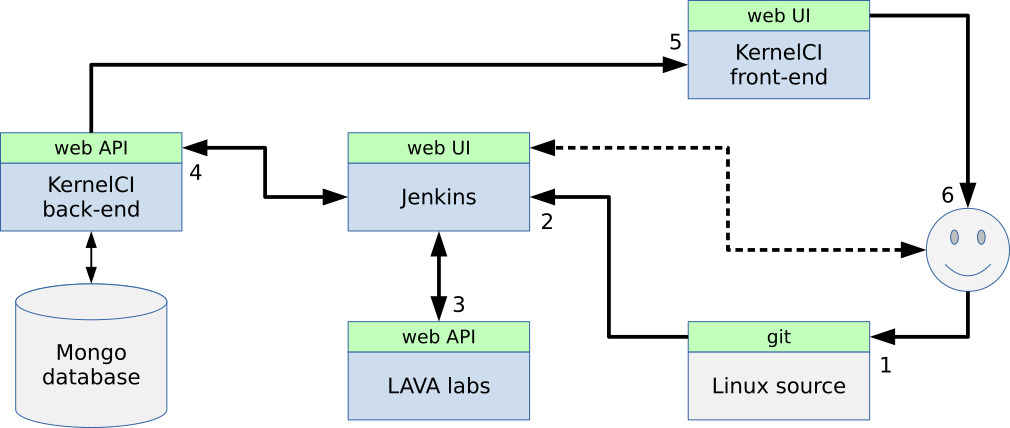
\includegraphics[width=7cm]{10_2018_Shadura1.png}
  %\caption{Блок-схема примерной системы распознавания РОГ}
  \label{Shadura1}
\end{figure}
\end{center} 

Kernel CI combines multiple components in a pipeline:
\begin{itemize}
\item New code lands in the Linux kernel Git repository
\item Jenkins triggers the build process with multiple configurations
\item After build finishes, Jenkins submits LAVA jobs
\item LAVA boots the built Linux kernels
\item Results get pushed back to Kernel CI
\end{itemize}

This process is applied to the master branch, \textbf{next} branch, stable branches and various topic branches (e.g. arm-soc, adnroid etc)

\subsection*{How to use LAVA}

There are two types of configuration files controlling LAVA: job definitions and test definitions. Job definitions tell LAVA how to get a specific series of test running on a device, i.e. what ot boot on the device, how to set up the environment and what tests to run. Test definitions define the tests themselves: what commands need to be run to get the test executed.

\subsubsection*{LAVA job definitions}

LAVA jobs are described using a YAML-based job definition\linebreak language. They define some job metadata and a series of actions. Each action tells LAVA to deploy an OS, boot it or run some tests in it. If needed, actions may repeat, so that the process consists of multiple stages.

In the simplest case, a job may look like this:

\begin{verbatim}
device_type: bcm2836-rpi-2-b
job_name: boot test
visibility: public\end{verbatim}\begin{verbatim}timeouts:
  job:
    minutes: 10\end{verbatim}\begin{verbatim}actions:
- deploy:
    to: tftp
    kernel:
      url: https://server.org/path/to/zImage
      type: zimage
    dtb:
      url: https://server.org/path/to/raspberry-pi-2b.dtb
    ramdisk:
      url: https://server.org/path/to/ramdisk-armhf.cpio.gz
      compression: gz
    os: oe\end{verbatim}\begin{verbatim}- boot:
    method: u-boot
    commands: ramdisk
    auto_login:
      login_prompt: 'root login:'
      username: root
    prompts: ['# ']\end{verbatim}This simple job just boots the kernel without running any actual tests. LAVA should already know how to boot Raspberry Pi 2 Model B given URLs to the kernel, DTB and the ramdisk. Alternatively, it can be booted from e.g. NFS filesystem.

It’s a bit more complicated when the target OS cannot be put on NFS or when you need to test the actual target images, as is the case with Apertis, a Debian derivative for automotive use. LAVA cannot boot directly into the flash or SD card image, so we need to split the boot process in two stages: the first one boots a minimal Linux system which puts the image onto a permanent storage, and then reboots into that image.

\begin{verbatim}
- boot:
    namespace: flash
    timeout:
      minutes: 10
    method: u-boot
    commands: nfs
    prompts:
    - 'root@stretch:'
    auto_login:
      login_prompt: 'stretch login:'
      username: root
      password_prompt: 'Password:'
      password: password
      
- deploy:
    namespace: system
    timeout:
      minutes: 20
    to: usb
    device: sd-card
    tool:
      prompts: ['copying time: [0-9ms\.\ ]+, copying speed 
[0-9\.]+ MiB\/sec']
    images:
      image:
        url: https://images.apertis.org/daily/18.09/
20180801.0/arm64/target/apertis_18.09-target-
arm64-uboot_20180801.0.img.gz
      bmap:
        url: https://images.apertis.org/daily/18.09/
20180801.0/arm64/target/apertis_18.09-target-arm64-
uboot_20180801.0.img.bmap
    uniquify: false
    os: ubuntu
    writer:
      tool: /usr/bin/bmaptool
      options: copy {DOWNLOAD_URL} {DEVICE}
      prompt: 'bmaptool: info'\end{verbatim}


Here, the first stage is put into a namespace called \verb@flash@, while the second one is called \verb@system@. In the first stage, LAVA deploys a minimal Debian stretch system, which contains \verb@bmaptool@, a tool which can effectively write images with big holes, which is what most OS images are. LAVA sets up a root FS to be available over NFS and boots into it, entering the next stage. In the secondary stage, \verb@deploy@ action tells LAVA to download the image and write it to the SD card using \verb@bmaptool@. Another \verb@boot@ section afterwards instructs LAVA to reboot into the newly flashed image.

\begin{verbatim}
- test:
    timeout:
      minutes: 15
    namespace: system
    name: sanity-check
    definitions:
      - repository: https://gitlab.apertis.org/
infrastructure/apertis-tests
        revision: master
        from: git
        path: common/sanity-check.yaml
        name: sanity-check-initial
      - repository: https://gitlab.apertis.org/
infrastructure/apertis-tests
        revision: master
        from: git
        path: misc/add-repo.yaml
        name: add-repo\end{verbatim}


The \verb@test@ action tells LAVA what tests to run and where to find them.

\subsubsection*{LAVA test definitions}

Test definitions specify the test metadata and tell the LAVA test runner what dependencies the test requires, what commands to run and how to parse the output.

\begin{verbatim}
metadata:
  name: check-dbus-services
  format: "Lava-Test-Shell Test Definition 1.0"
  description: "Sanity-check all installed D-Bus services"
  maintainer: "simon.mcvittie@collabora.co.uk"
  scope:
  - functional
  devices:
  - i386
  environment:
  - lava-test-shell\end{verbatim}\begin{verbatim}install:
  deps:
  - apertis-tests
  - dbus-tests\end{verbatim}\begin{verbatim}run:
  steps:
  - common/run-test-in-systemd --user=user dbus/check-
dbus-services
  - common/run-test-in-systemd dbus/check-dbus-services\end{verbatim}\begin{verbatim}parse:
  pattern: 'RESULT:(?P<result>\w+):
(?P<test_case_id>[^:]+):'
  # LAVA doesn't seem to have the concept of an expected failure,
  # so calling it skipped is the next best thing
  fixupdict:
    xfail: skip\end{verbatim}

\subsection*{Integrating LAVA}

\begin{center}
\begin{figure}[h!]
  \centering
  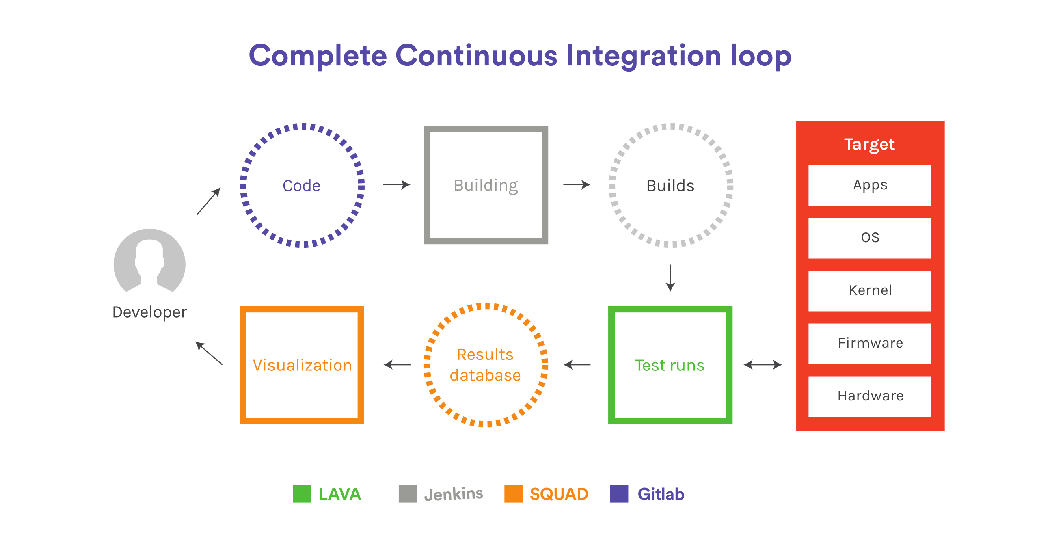
\includegraphics[width=8cm]{10_2018_Shadura2.png}
  %\caption{Блок-схема примерной системы распознавания РОГ}
  \label{Shadura2}
\end{figure}
\end{center} 

LAVA can be integrated with software such as SQUAD to store and visualise the test results. For Apertis, we have written a bridge webservice which collects results related to a series of images and posts the results to the bug tracker, and also sends email and chat notifications.

\end{document}

\documentclass[10pt, a5paper]{article}
\usepackage{pdfpages}
\usepackage{parallel}
\usepackage[T2A]{fontenc}
\usepackage{ucs}
\usepackage[utf8x]{inputenc}
\usepackage[polish,english,russian]{babel}
\usepackage{hyperref}
\usepackage{rotating}
\usepackage[inner=2cm,top=1.8cm,outer=2cm,bottom=2.3cm,nohead]{geometry}
\usepackage{listings}
\usepackage{graphicx}
\usepackage{wrapfig}
\usepackage{longtable}
\usepackage{indentfirst}
\usepackage{array}
\newcolumntype{P}[1]{>{\raggedright\arraybackslash}p{#1}}
\frenchspacing
\usepackage{fixltx2e} %text sub- and superscripts
\usepackage{icomma} % коскі ў матэматычным рэжыме
\PreloadUnicodePage{4}

\newcommand{\longpage}{\enlargethispage{\baselineskip}}
\newcommand{\shortpage}{\enlargethispage{-\baselineskip}}

\def\switchlang#1{\expandafter\csname switchlang#1\endcsname}
\def\switchlangbe{
\let\saverefname=\refname%
\def\refname{Літаратура}%
\def\figurename{Іл.}%
}
\def\switchlangen{
\let\saverefname=\refname%
\def\refname{References}%
\def\figurename{Fig.}%
}
\def\switchlangru{
\let\saverefname=\refname%
\let\savefigurename=\figurename%
\def\refname{Литература}%
\def\figurename{Рис.}%
}

\hyphenation{admi-ni-stra-tive}
\hyphenation{ex-pe-ri-ence}
\hyphenation{fle-xi-bi-li-ty}
\hyphenation{Py-thon}
\hyphenation{ma-the-ma-ti-cal}
\hyphenation{re-ported}
\hyphenation{imp-le-menta-tions}
\hyphenation{pro-vides}
\hyphenation{en-gi-neering}
\hyphenation{com-pa-ti-bi-li-ty}
\hyphenation{im-pos-sible}
\hyphenation{desk-top}
\hyphenation{elec-tro-nic}
\hyphenation{com-pa-ny}
\hyphenation{de-ve-lop-ment}
\hyphenation{de-ve-loping}
\hyphenation{de-ve-lop}
\hyphenation{da-ta-ba-se}
\hyphenation{plat-forms}
\hyphenation{or-ga-ni-za-tion}
\hyphenation{pro-gramming}
\hyphenation{in-stru-ments}
\hyphenation{Li-nux}
\hyphenation{sour-ce}
\hyphenation{en-vi-ron-ment}
\hyphenation{Te-le-pathy}
\hyphenation{Li-nux-ov-ka}
\hyphenation{Open-BSD}
\hyphenation{Free-BSD}
\hyphenation{men-ti-on-ed}
\hyphenation{app-li-ca-tion}

\def\progref!#1!{\texttt{#1}}
\renewcommand{\arraystretch}{2} %Іначай формулы ў матрыцы зліпаюцца з лініямі
\usepackage{array}

\def\interview #1 (#2), #3, #4, #5\par{

\section[#1, #3, #4]{#1 -- #3, #4}
\def\qname{LVEE}
\def\aname{#1}
\def\q ##1\par{{\noindent \bf \qname: ##1 }\par}
\def\a{{\noindent \bf \aname: } \def\qname{L}\def\aname{#2}}
}

\def\interview* #1 (#2), #3, #4, #5\par{

\section*{#1\\{\small\rm #3, #4. #5}}

\def\qname{LVEE}
\def\aname{#1}
\def\q ##1\par{{\noindent \bf \qname: ##1 }\par}
\def\a{{\noindent \bf \aname: } \def\qname{L}\def\aname{#2}}
}

\switchlang{ru}
\begin{document}
\title{Разработка архитектуры Game-stream платформы на основе OpenSource компонентов\footnote{\url{arol90@gmail.com}, \url{https://lvee.org/en/abstracts/276}}}
\author{Антон Новиков, Минск, Belarus}
\maketitle
\begin{abstract}
A game stream service development and architecture specifics are covered with focus on the open source components. Personal experience of building such service is covered, including compo\-nents choice and resulting performance.
\end{abstract}
\section*{Введение}

В настоящее время активно развивается направление games as a service. Основной задачей таких сервисов является предоставление возможности потребителю быстро и, главное, не имея достаточных вычислительных ресурсов, получить игровой опыт неотличимый от запуска игры на своем компьютере.

Подобные сервисы существуют достаточно давно, но зачастую являются проприетарными и недоступными для использования иначе чем в потребительских целях на платной основе.

%%\begin{center}
%%\begin{figure}[h!]
%%  \centering
%%  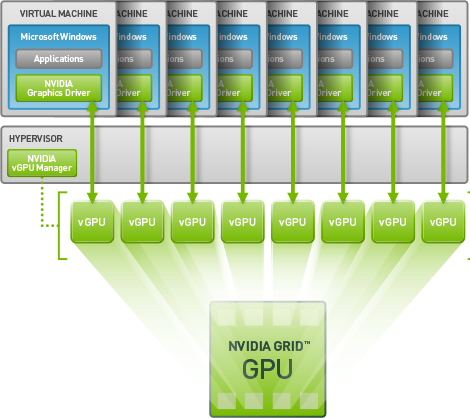
\includegraphics[width=5.5cm]{11_2018_Novikov1}
%%%  \caption{~}
%%%  \label{fig:Kharkevich1}
%%\end{figure}
%%\end{center} 

Главной предпосылкой появления возможности трансляции игр в виде видео-потока на компьютер пользователя стало появление в системах виртуализации технологии проброса графического адаптера (либо части графического адаптера) в виртуальную машину. Эта технология обширно используется в профессиональной среде с CAD-приложениями, давая возможность разделения одного мощного графического адаптера на несколько потребителей.

Также существуют и другие возможности применения данной схемы – например, математическое расчеты на GPU, построение 3D-моделей, рендеринг видео и другие.

Разрабатываемая автором по данной схеме система потокового game-сервиса является универсальной и полнофункциональной. Её особенности раскрыты ниже.

\section*{Архитектура}

Архитектура подобного рода сервисов зачастую является <<конструктором>> из множества различных по функциональному назначению модулей и компонентов:
\begin{itemize}
\item аппаратная платформа;
\item ОС для аппаратной платформы;
\item ОС для виртуальных машин;
\item средства управления и оркестрации;
\item средства кластеризации и распределения нагрузок;
\item приложения.
\end{itemize}

\section*{Front-end и биллинг}

В качестве опорных точек были выбраны некоторые основные аспекты:
\begin{itemize}
\item Каждое приложение~--- это отдельная виртуальная машина.
\item Все функции по обслуживанию виртуальных машин берёт на себя система виртуализации.
\item ОС для запуска приложения должна быть стабильным LTS-дистрибутивом GNU/Linux.
\item Система виртуализации имеет функционал частичного проброса графического адаптера.
\item Возможность использования как на физических серверах в собственном ЦОД, так и на арендованных выделенных серверах облачных провайдеров.
\end{itemize}
\section*{Обоснование выбора компонентов}

\subsection*{Аппаратная платформа} 
В зависимости от сложности приложений необходимо учитывать вычислительные мощности; поэтому было разработано несколько концепций вычислительного сервера и его усредненная модель:
\begin{itemize}
\item 2 CPU Intel Xeon 8 core 2.66 ГГц; 
\item 128 GB RAM;
\item 4 карты Nvidia Tesla P100;
\item корпус с возможностью установки графических карт.
\end{itemize}

\subsection*{ОС для аппаратной платформы}
Выбор системы виртуализации первоочередно обоснован возможностью проброса графического адаптера в ВМ, и самой продвинутой по этой части из свободных платформ на данный момент является XCP-next generation (основанный на базе XEN Server, под лицензией GNU General Public License). Также и все библиотеки Nvidia, необходимые для осуществления требуемого функционала, распространяются на свободной основе.

Система имеет возможности частичного и полного проброса, встроенные средства управления кластером, мониторинга, резервного копирования и полностью совместима с гипервизором, используемым в AWS, что дает возможность развертывания платформы в арендованных облаках.

В дополнение к функционалу гипервизора была добавлена система оркестрации XenOrchestra (также под свободной лицензией, AGPLv3).

\subsection*{ОС для виртуальных машин}
Для запуска большинства игр из библиотеки Steam, которые совместимы с ОС Linux, необходима Debian-подобная система (Steam OS). Именно стабильная версия ОС Debian 9 легла в основу золотого образа. Также могли бы быть использованы и другие ОС: SteamOS в режиме киоска, Ubuntu 16.04 LTS для разработки и создания игр на графическом движке Unreal Engine 4.

Во всей архитектуре использована концепция <<одна игра = одна виртуальная машина>>, такой подход позволяет легко клонировать и перемещать игры внутри вычислительного кластера, разделять ресурсы, и быстро запускать игры по запросу пользователя.

\subsection*{Front-end и биллинг} 
В отношении клиентской части перед командой разработчиков стояла задача разработки системы биллинга и конечного клиентского приложения, но существует возможность использования и готовых решений.
\subsection*{Стрим-приложения}
Непосредственно захват изображения, рендеринг, кодирование его для передачи производились на графическом адаптере. Новые поколения графических карт имеют возможность одновременной работы как рендерера, так и энкодера – при помощи всего лишь стандартного функционала. Для программной обработки были использованы свободные библиотеки OpenBroadcasterSoftware (GNU General Public License, version 2) и стандартный функционал приложения.

\section*{Сравнение производительности}
При развёртывании стенда для тестирования производительности полученной системы и сравнения её с аналогами были использованы также готовые виртуальные машины на AWS, основанные на Windows 2016 Server. Результаты тестирования отличались на уровне погрешности, но следует заметить, что платформа, основанная на свободном ПО, отличается большей гибкостью и возможностями применения, проприетарная же платформа ограничена играми. Если использовать платформу только для игр, то платформа на основе Windows находится в преимуществе исключительно из-за количества доступных игр.

\section*{Заключение}
Разработанная архитектура прошла все этапы тестирования и успешно используется для различных целей, легко адаптируемая под задачи: Разработка игр, стрим игр, обработка 3d графики, CAD приложения, ДЕМО 3d приложения, вычисления с использованием GPU. 
Легкость адаптации, бесконечное горизонтальное масштабирование, возможность использоваться на арендованных облаках и гибридных облаках делают систему универсальной платформой и мощным инструментом собранным исключительно из свободных компонентов.

\end{document}

\documentclass[10pt, a5paper]{article}
\usepackage{pdfpages}
\usepackage{parallel}
\usepackage[T2A]{fontenc}
\usepackage{ucs}
\usepackage[utf8x]{inputenc}
\usepackage[polish,english,russian]{babel}
\usepackage{hyperref}
\usepackage{rotating}
\usepackage[inner=2cm,top=1.8cm,outer=2cm,bottom=2.3cm,nohead]{geometry}
\usepackage{listings}
\usepackage{graphicx}
\usepackage{wrapfig}
\usepackage{longtable}
\usepackage{indentfirst}
\usepackage{array}
\newcolumntype{P}[1]{>{\raggedright\arraybackslash}p{#1}}
\frenchspacing
\usepackage{fixltx2e} %text sub- and superscripts
\usepackage{icomma} % коскі ў матэматычным рэжыме
\PreloadUnicodePage{4}

\newcommand{\longpage}{\enlargethispage{\baselineskip}}
\newcommand{\shortpage}{\enlargethispage{-\baselineskip}}

\def\switchlang#1{\expandafter\csname switchlang#1\endcsname}
\def\switchlangbe{
\let\saverefname=\refname%
\def\refname{Літаратура}%
\def\figurename{Іл.}%
}
\def\switchlangen{
\let\saverefname=\refname%
\def\refname{References}%
\def\figurename{Fig.}%
}
\def\switchlangru{
\let\saverefname=\refname%
\let\savefigurename=\figurename%
\def\refname{Литература}%
\def\figurename{Рис.}%
}

\hyphenation{admi-ni-stra-tive}
\hyphenation{ex-pe-ri-ence}
\hyphenation{fle-xi-bi-li-ty}
\hyphenation{Py-thon}
\hyphenation{ma-the-ma-ti-cal}
\hyphenation{re-ported}
\hyphenation{imp-le-menta-tions}
\hyphenation{pro-vides}
\hyphenation{en-gi-neering}
\hyphenation{com-pa-ti-bi-li-ty}
\hyphenation{im-pos-sible}
\hyphenation{desk-top}
\hyphenation{elec-tro-nic}
\hyphenation{com-pa-ny}
\hyphenation{de-ve-lop-ment}
\hyphenation{de-ve-loping}
\hyphenation{de-ve-lop}
\hyphenation{da-ta-ba-se}
\hyphenation{plat-forms}
\hyphenation{or-ga-ni-za-tion}
\hyphenation{pro-gramming}
\hyphenation{in-stru-ments}
\hyphenation{Li-nux}
\hyphenation{sour-ce}
\hyphenation{en-vi-ron-ment}
\hyphenation{Te-le-pathy}
\hyphenation{Li-nux-ov-ka}
\hyphenation{Open-BSD}
\hyphenation{Free-BSD}
\hyphenation{men-ti-on-ed}
\hyphenation{app-li-ca-tion}

\def\progref!#1!{\texttt{#1}}
\renewcommand{\arraystretch}{2} %Іначай формулы ў матрыцы зліпаюцца з лініямі
\usepackage{array}

\def\interview #1 (#2), #3, #4, #5\par{

\section[#1, #3, #4]{#1 -- #3, #4}
\def\qname{LVEE}
\def\aname{#1}
\def\q ##1\par{{\noindent \bf \qname: ##1 }\par}
\def\a{{\noindent \bf \aname: } \def\qname{L}\def\aname{#2}}
}

\def\interview* #1 (#2), #3, #4, #5\par{

\section*{#1\\{\small\rm #3, #4. #5}}

\def\qname{LVEE}
\def\aname{#1}
\def\q ##1\par{{\noindent \bf \qname: ##1 }\par}
\def\a{{\noindent \bf \aname: } \def\qname{L}\def\aname{#2}}
}

\begin{document}
\title{Низкоуровневый взгляд на динамические ELF-библиотеки\footnote{\url{punkofnewsociety@gmail.com}, \url{https://lvee.org/en/abstracts/280}, материал распространяется под лицензией Attribution 4.0 International (CC BY 4.0)}}
\author{Uladzislau Zhauniarovich, Minsk, Belarus}
\maketitle
\begin{abstract}
Complex applications work with dynamically linked libraries. Statically linked applications would be very large and have lack of flexibility as with dynamic libraries, because one library can be used by several applications at once.
The purpose of this report is precisely to focus on all low-level features of working with these libraries, including such mechanisms like 
ELF sections, symbol relocations, GOT(global offset table), PLT(procedure linkage table).
\end{abstract}
\section*{Введение}

На примере языка программирования Си можно выделить три основных этапа с момента написания программного кода до работы получившейся программы в операционной системе. 
Это препроцессинг, компиляция, компоновка/линковка. Остановимся на последнем этапе. К этому времени инструкции в процессе компиляции в  основном сгенерированы.  Компоновщик~--- это программа, которая выбирает адреса для всех символов(глобальные переменные и функции, либо вспомогательные debug-символы). Без компоновщика мы бы не могли делать раздельную компиляцию. Много обьектных файлов не нужно перекомпилировать с самого начала, если в них нету изменений и пересборка идет только в файлах с изменениями(прим. open office, linux kernel).

ELF~--- Executable and Linkable Format. Эти файлы можно разделить на три категории:

\begin{itemize}
  \item Relocatable files~--- .o (то что получается после компиляции) является элементом static libraries (.a), т.е. может включать 1 или больше.
  \item Executable~--- программы после этапа линковки, готовые к запуску.
  \item Shared~--- .so dynamic libraries, они должны быть скомпонованы с запускаемым файлом в run-time.
\end{itemize}

Релокация~--- это процесс подстановки символу его адреса. 

Static linker превращает первую категорию во вторую или третью.

Dynamic linker подготавливает третью к выполнению.

\section*{Инструменты для анализа бинарных файлов}

Список таких инструментов включает:

\begin{itemize}
  \item readelf~--- получение специфичной для формата ELF информации.
  \item objdump~--- дизассемблер, позволяет исследовать обьектные файлы разных форматов.
  \item nm~--- просмотр символов, которые есть в ELF-файле.
\end{itemize}

В набор GNU Binutils также входят elfedit, elfdump и др., но в данном контексте они не понадобятся.

\section*{Структура ELF, содержимое секций}

ELF-файл содержит 3 заголовка~--- File Header, Program Header, и Section Header.
Заголовок ELF-файла содержит magic number 7f 45 4c 46 ( 7f + ascii коды букв ELF) и указатели на Program Header и Section Header.

Program Header формируется при помощи компоновщика и содержит 
информацию о сегментах. Сегменты~--- это регионы памяти, которые содержат некоторое количество секций.

Section Header содержит информацию про секции .text .data .bss .rodata и множество служебных секций .symtab .line .strtab .debug .got .got.plt. Он необходим для линковки.
\newpage
\begin{center}
\begin{figure}[h!]
  \centering
  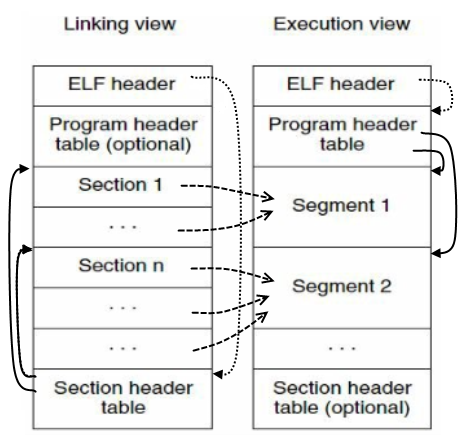
\includegraphics[width=7cm]{12_2018_Zhauniarovich1.png}
  %\caption{Блок-схема примерной системы распознавания РОГ}
  \label{Zhauniarovich1}
\end{figure}
\end{center} 

\section*{Релокации, GOT, PLT}

Когда линкер создает разделяемую библиотеку, он заранее не знает, в каком месте в памяти она будет загружена. Из-за этого делать ссылки на данные и код внутри библиотеки проблематично: непонятно, как создавать ссылку, чтобы она указывала в правильное место после того, как библиотека будет загружена.

В Linux и в ELF существует два главных способа решить эту проблему:

\begin{itemize}
  \item релокация во время загрузки (load-time relocation);
  \item код, не зависящий от адреса (position-independent code, PIC).
\end{itemize}

Релокация во время загрузки~--- это очень простой и прямолинейный метод. И он работает. Но PIC гораздо более популярен на данный момент и является рекомендуемым способом создания разделяемых библиотек.

У load-time relocation есть проблемы: она занимает время, и секция text (содержащая машинный код) уже не подходит для разделения между процессами.

Поэтому существует такая модель, как Global Offset Table. 
GOT~--- это просто таблица с адресами, которая находится в секции data.

Предположим, что какая-то инструкция в секции code хочет обратиться к переменной. Вместо того, чтобы обратится к ней через абсолютный адрес (который потребует релокации), она обращается к записи в GOT. Поскольку GOT имеет строго определённое место в секции data, и линкер знает о нём, это обращение тоже является относительным. А запись в GOT уже содержит абсолютный адрес переменной:

\begin{center}
\begin{figure}[h!]
  \centering
  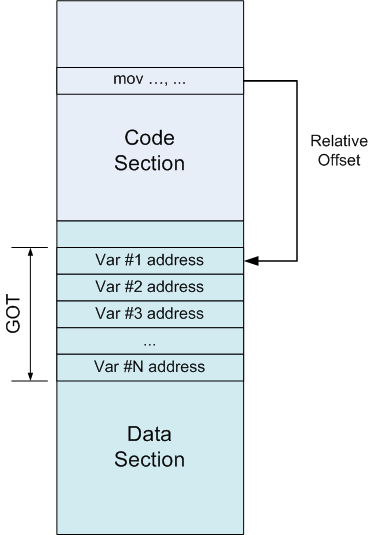
\includegraphics[width=5cm]{12_2018_Zhauniarovich2.png}
  %\caption{Блок-схема примерной системы распознавания РОГ}
  \label{Zhauniarovich2}
\end{figure}
\end{center} 

Однако суть разделяемых библиотек на сегодняшний день в том, что в них может содержаться 10 000 различных функций, но использовать оттуда мы, например, будем лишь № 1 или № 4. Чтобы каждый раз подгружать абсолютно все функции в GOT, мы используем процедуру <<ленивого связывания>>, т.е. связывание функции из библиотеки с программой происходит при непосредственном вызове её. Помогает в этом механизм Procedure Linkage Table (PLT).

PLT~--- это часть секции text в бинарнике, состоящая из набора элементов (один элемент на одну внешнюю функцию, которую вызывает библиотека). Каждый элемент в PLT~--- это небольшой кусок выполняемого машинного кода. Вместо вызова функции напрямую вызывается кусок кода из PLT, который уже сам вызывает функцию. Такой подход часто называют <<трамплином>>. Каждый элемент из PLT имеет собственный элемент в GOT, который содержит реальное смещение для функции (конечно после того как загрузчик определит её).

\begin{center}
\begin{figure}[h!]
  \centering
  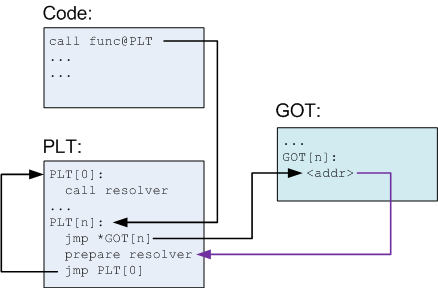
\includegraphics[width=5cm]{12_2018_Zhauniarovich3.png}
  %\caption{Блок-схема примерной системы распознавания РОГ}
  \label{Zhauniarovich3}
\end{figure}
\end{center} 

В коде вызывается функция func. Компилятор переводит этот вызов в вызов func@plt, который является одним из элементов PLT. После этого идет обращение в GOT, и с учетом того что функция вызывалась в первый раз~--- управление передаётся обратно PLT, где т. н. resolver устанавливает связь между названием функции и её кодом из библиотеки. После такого первого связывания схема будет выглядеть немного по-другому:

\begin{center}
\begin{figure}[h!]
  \centering
  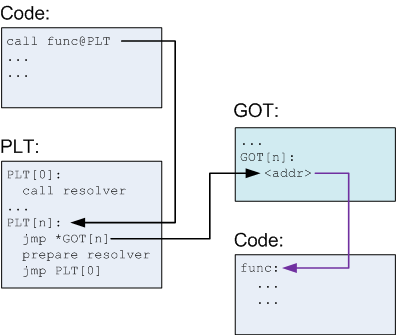
\includegraphics[width=5cm]{12_2018_Zhauniarovich4.png}
  %\caption{Блок-схема примерной системы распознавания РОГ}
  \label{Zhauniarovich4}
\end{figure}
\end{center} 

Библиотека при этом абсолютно не зависит от адреса, по которому она будет загружена: ведь единственное место, где используется абсолютный адрес~--- это GOT, а она находится в секции data и будет релоцирована загрузчиком во время загрузки. Даже PLT не зависит от адреса загрузки, так что она может находиться в секции text, доступной только для чтения.

\section*{Эксперимент с перенаправлением обращений к функциям из библиотек}

Наглядно продемонстрировать описанные процессы можно в ходе эксперимента с использованием предварительно написанной демонстрационной программы, функциональность которой должна включать:

\begin{itemize}
  \item создание паттерна <<Proxy>> для вызова функций (которые, в свою очередь, используют системные функции) из заранее откопилированных (пользовательских) библиотек без их прямого изменения;
  \item перенаправление их вызовов в свой интерфейс, для дальнейшего вызова тех самых системных функций из пользовательских библиотек.
\end{itemize}

\end{document}

\documentclass[10pt, a5paper]{article}
\usepackage{pdfpages}
\usepackage{parallel}
\usepackage[T2A]{fontenc}
\usepackage{ucs}
\usepackage[utf8x]{inputenc}
\usepackage[polish,english,russian]{babel}
\usepackage{hyperref}
\usepackage{rotating}
\usepackage[inner=2cm,top=1.8cm,outer=2cm,bottom=2.3cm,nohead]{geometry}
\usepackage{listings}
\usepackage{graphicx}
\usepackage{wrapfig}
\usepackage{longtable}
\usepackage{indentfirst}
\usepackage{array}
\newcolumntype{P}[1]{>{\raggedright\arraybackslash}p{#1}}
\frenchspacing
\usepackage{fixltx2e} %text sub- and superscripts
\usepackage{icomma} % коскі ў матэматычным рэжыме
\PreloadUnicodePage{4}

\newcommand{\longpage}{\enlargethispage{\baselineskip}}
\newcommand{\shortpage}{\enlargethispage{-\baselineskip}}

\def\switchlang#1{\expandafter\csname switchlang#1\endcsname}
\def\switchlangbe{
\let\saverefname=\refname%
\def\refname{Літаратура}%
\def\figurename{Іл.}%
}
\def\switchlangen{
\let\saverefname=\refname%
\def\refname{References}%
\def\figurename{Fig.}%
}
\def\switchlangru{
\let\saverefname=\refname%
\let\savefigurename=\figurename%
\def\refname{Литература}%
\def\figurename{Рис.}%
}

\hyphenation{admi-ni-stra-tive}
\hyphenation{ex-pe-ri-ence}
\hyphenation{fle-xi-bi-li-ty}
\hyphenation{Py-thon}
\hyphenation{ma-the-ma-ti-cal}
\hyphenation{re-ported}
\hyphenation{imp-le-menta-tions}
\hyphenation{pro-vides}
\hyphenation{en-gi-neering}
\hyphenation{com-pa-ti-bi-li-ty}
\hyphenation{im-pos-sible}
\hyphenation{desk-top}
\hyphenation{elec-tro-nic}
\hyphenation{com-pa-ny}
\hyphenation{de-ve-lop-ment}
\hyphenation{de-ve-loping}
\hyphenation{de-ve-lop}
\hyphenation{da-ta-ba-se}
\hyphenation{plat-forms}
\hyphenation{or-ga-ni-za-tion}
\hyphenation{pro-gramming}
\hyphenation{in-stru-ments}
\hyphenation{Li-nux}
\hyphenation{sour-ce}
\hyphenation{en-vi-ron-ment}
\hyphenation{Te-le-pathy}
\hyphenation{Li-nux-ov-ka}
\hyphenation{Open-BSD}
\hyphenation{Free-BSD}
\hyphenation{men-ti-on-ed}
\hyphenation{app-li-ca-tion}

\def\progref!#1!{\texttt{#1}}
\renewcommand{\arraystretch}{2} %Іначай формулы ў матрыцы зліпаюцца з лініямі
\usepackage{array}

\def\interview #1 (#2), #3, #4, #5\par{

\section[#1, #3, #4]{#1 -- #3, #4}
\def\qname{LVEE}
\def\aname{#1}
\def\q ##1\par{{\noindent \bf \qname: ##1 }\par}
\def\a{{\noindent \bf \aname: } \def\qname{L}\def\aname{#2}}
}

\def\interview* #1 (#2), #3, #4, #5\par{

\section*{#1\\{\small\rm #3, #4. #5}}

\def\qname{LVEE}
\def\aname{#1}
\def\q ##1\par{{\noindent \bf \qname: ##1 }\par}
\def\a{{\noindent \bf \aname: } \def\qname{L}\def\aname{#2}}
}

\begin{document}
\title{DevOps для QA на примере Java Enterprise проекта\footnote{\url{garanin@itworks.by}, \url{https://www.linkedin.com/in/garaninromanbrest/}, \url{skype://garanin.roman.brest}, \url{https://lvee.org/en/abstracts/284}}}
\author{Гаранин Роман, руководитель отдела тестирования\\ ООО <<Итворкс>>, г. Брест, Беларусь}
\maketitle
\begin{abstract}
In this report, I would like to share the experience of using the DevOps philosophy in our company for one of the projects in the financial sphere. Emphasis will be placed on the work of the quality assurance department, because exactly because of the large number of questions there and the increased quality requirements, the philosophy of DevOps was applied there in the first place.
\end{abstract}
В этом докладе хотел бы поделиться опытом применения философии DevOps: инструментов котейнеризации и непрерывного развёртывания в нашей компании для одного из проектов в финансовой сфере. Упор будет сделан именно на работу отдела QA, потому как именно из-за большого количества вопросов и повышенных требований к качеству философия DevOps была применена там в первую очередь.

Также одна из целей данного доклада~--- это получение обратной связи от участников сообщества (критика, комментарии, предложения по оптимизации).

\subsection*{1. Постановка задачи и описание тестируемого проекта}

Реальный проект большой и сложный, но для лучшего понимания ситуации представим, что у нас имеется портал для  выдачи займов физическим лицам: проверка возможности выдачи займа, оформление соответствующих документов и сопутствующие задачи. Пользователи/клиенты работают с порталом через браузер.

Проект представляет собой J2EE решение, которое состоит из компонентов:

\begin{itemize}
  \item два сервера приложений JBoss (бэк-сервер и фронт-сервер)
  \item ядро системы на Java
  \item процессная часть на JBoss JBPM, куда вынесены бизнес"=процессы
  \item отчеты (JasperReports)
  \item пользовательские формы для отображения в браузере
  \item коннекторы к другим компонентам инфраструктуры (базы данных, сервисы и проч.)
  \item файлы настроек
  \item и многое другое\ldots{}
\end{itemize}

Используемая база данных: Oracle 11g (используется у заказчика).
Исходные коды проекта хранятся в системе контроля версий Mercurial.

Два сервера приложений проекта это:

\begin{itemize}
  \item бэк-сервер~--- с ним работают специалисты заказчика;
  \item фронт-сервер~--- с ним работают клиенты заказчика (через браузер или через мобильное приложение).
\end{itemize}

Упрощенная архитектура тестируемого приложения представлена на рис.~\ref{Gagarin1}:

\begin{center}
\begin{figure}[h!]
  \centering
  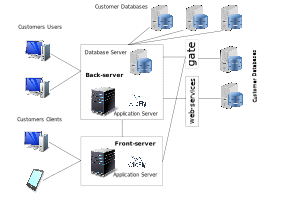
\includegraphics[width=7cm]{13_2018_Gagarin1}
  \caption{~}
  \label{Gagarin1}
\end{figure}
\end{center} 

Началось всё с того, что была поставлена задача по организации автоматических прогонов тестов (GUI) на проекте перед отправкой доработок заказчику. В ходе реализации выяснилось, что и исследовательское (ручное) тестирование также всё еще отнимает много времени и содержит много ручных повторяющихся действий, которые можно оптимизировать. Эти же причины стали препятствием на пути организации автоматизированного тестирования.

Цели, которые мы ставили:

2. Освободить сотрудников от рутинной подготовительной работы и дать им возможность сосредоточиться на задаче.

1. Организовать автоматическое выполнение тестов и быструю обратную связь от процесса развёртывания ПО в тестовой среде.

То есть начали делать цель 1, но пришли к тому, что приоритетнее цель 2 и без реализации цели 2 невозможно реализовать цель 1.

Основной болью сотрудников отдела QA была установка обновлений по доработкам: у каждого специалиста по тестированию были свой сервер JBoss на рабочей машине под Windows и общая база Oracle для тестирования на несколько специалистов. Такой подход приносил целый ряд проблем:

\begin{itemize}
  \item на одной общей базе одни доработки могли ломать другие;
  \item одному тестировщику нужны одни настройки, другому~--- другие, и вот так вот они перетирали друг друга;
  \item если тестировщик не тестировал какое-либо требование, то мог просто не знать об изменениях в некоторых процессах, коннекторах, формах, которые были в работе у другого тестировщика~--- в итоге получали проблему нарушения зависимостей;
и многое-многое другое\ldots{}
\end{itemize}

К тому же ситуация была такова, что при ручном тестировании значительная часть времени тратилась на <<что-то тут недонастроено>>, чем на тестирование нового функционала.

\subsection*{2. Инфраструктура DevOps}

Для решения всех этих проблем была подготовлена инфраструктура. В силу ряда причин (безопасность, конфиденциальность и проч.) решение не вынесено в облака, а полностью находится в локальной сети организации-разработчика. Упрощенно схема показана на рис.~\ref{Gagarin2}:

\begin{center}
\begin{figure}[h!]
  \centering
  \includegraphics[width=7cm]{13_2018_Gagarin2}
  \caption{~}
  \label{Gagarin2}
\end{figure}
\end{center} 

Рассмотрим ее подробнее.

Центральным звеном инфраструктуры является сервер CI под управлением OpenSUSE Linux, на котором установлен Docker. Весь основной софт (который мы рассмотрим ниже) работает в Docker-контейнерах.

Также на сервере CI запущен локальный реестр образов, откуда по сети забираются образы Docker.

Jenkins (Master) следит за обновлениями образов в репозитории Mercurial.

Кроме этого на сервере установлено различное вспомогательное ПО: база MySQL для нужд DevOps, Nginx для публикации отчетов, вспомогательные сервера Mercurial и многое другое. Надо отметить, что новое ПО на CI-сервер устанавливается лишь в крайнем случае~--- всё новое ПО выносится по возможности в контейнеры Docker~--- это очень упрощает дальнейшее сопровождение основной системы и образов.

Частями инфраструктуры также являются:

\begin{itemize}
  \item другие сетевые машины на CentOS для нужд тестирования и отладки, а также по настоящему <<физическая>> машина для запуска тестов мобильного приложения (так как эмуляторы Android не работают на виртуальных машинах);
  \item сетевые базы Oracle 11g для отладки.
\end{itemize}

Рабочее место специалиста по тестированию включает следующее обязательное ПО:

\begin{itemize}
  \item Docker Toolbox~--- набор инструментов для возможности запуска Docker на Windows 10;
  \item Oracle 11g Express Edition~--- локальная база для тестирования, то есть вместо общей сетевой базы у каждого тестировщика появилась своя собственная база, где настройки никто не мог поломать;
  \item Клиент Hg/Mercurial для работы с репозиторием.
\end{itemize}

В Docker-контейнере QA-специалиста запущен Docker-образ с OpenSUSE Linux, где и работает тестируемое приложение.

\subsection*{3. Контейнеризация}

Как было отмечено выше~--- всё основное ПО располагается в контейнерах Docker. Причем в образы кроме тестируемого приложения помещено различное вспомогательное ПО. Это удобно тем, что любой специалист может забрать на свою машину из образа готовое к использованию ПО со всеми настройками.

Организовано это следующим образом: сначала был разработан базовый образ (назовём его itw\_base), который включает минимально необходимое для работы ПО. На основе базового образа строятся другие образы. Для сокращения времени сборки наборы ПО были организованы в промежуточные образы. В результате получилась иерархия, которая упрощенно представлена на рис.~\ref{Gagarin3}:

\begin{center}
\begin{figure}[h!]
  \centering
  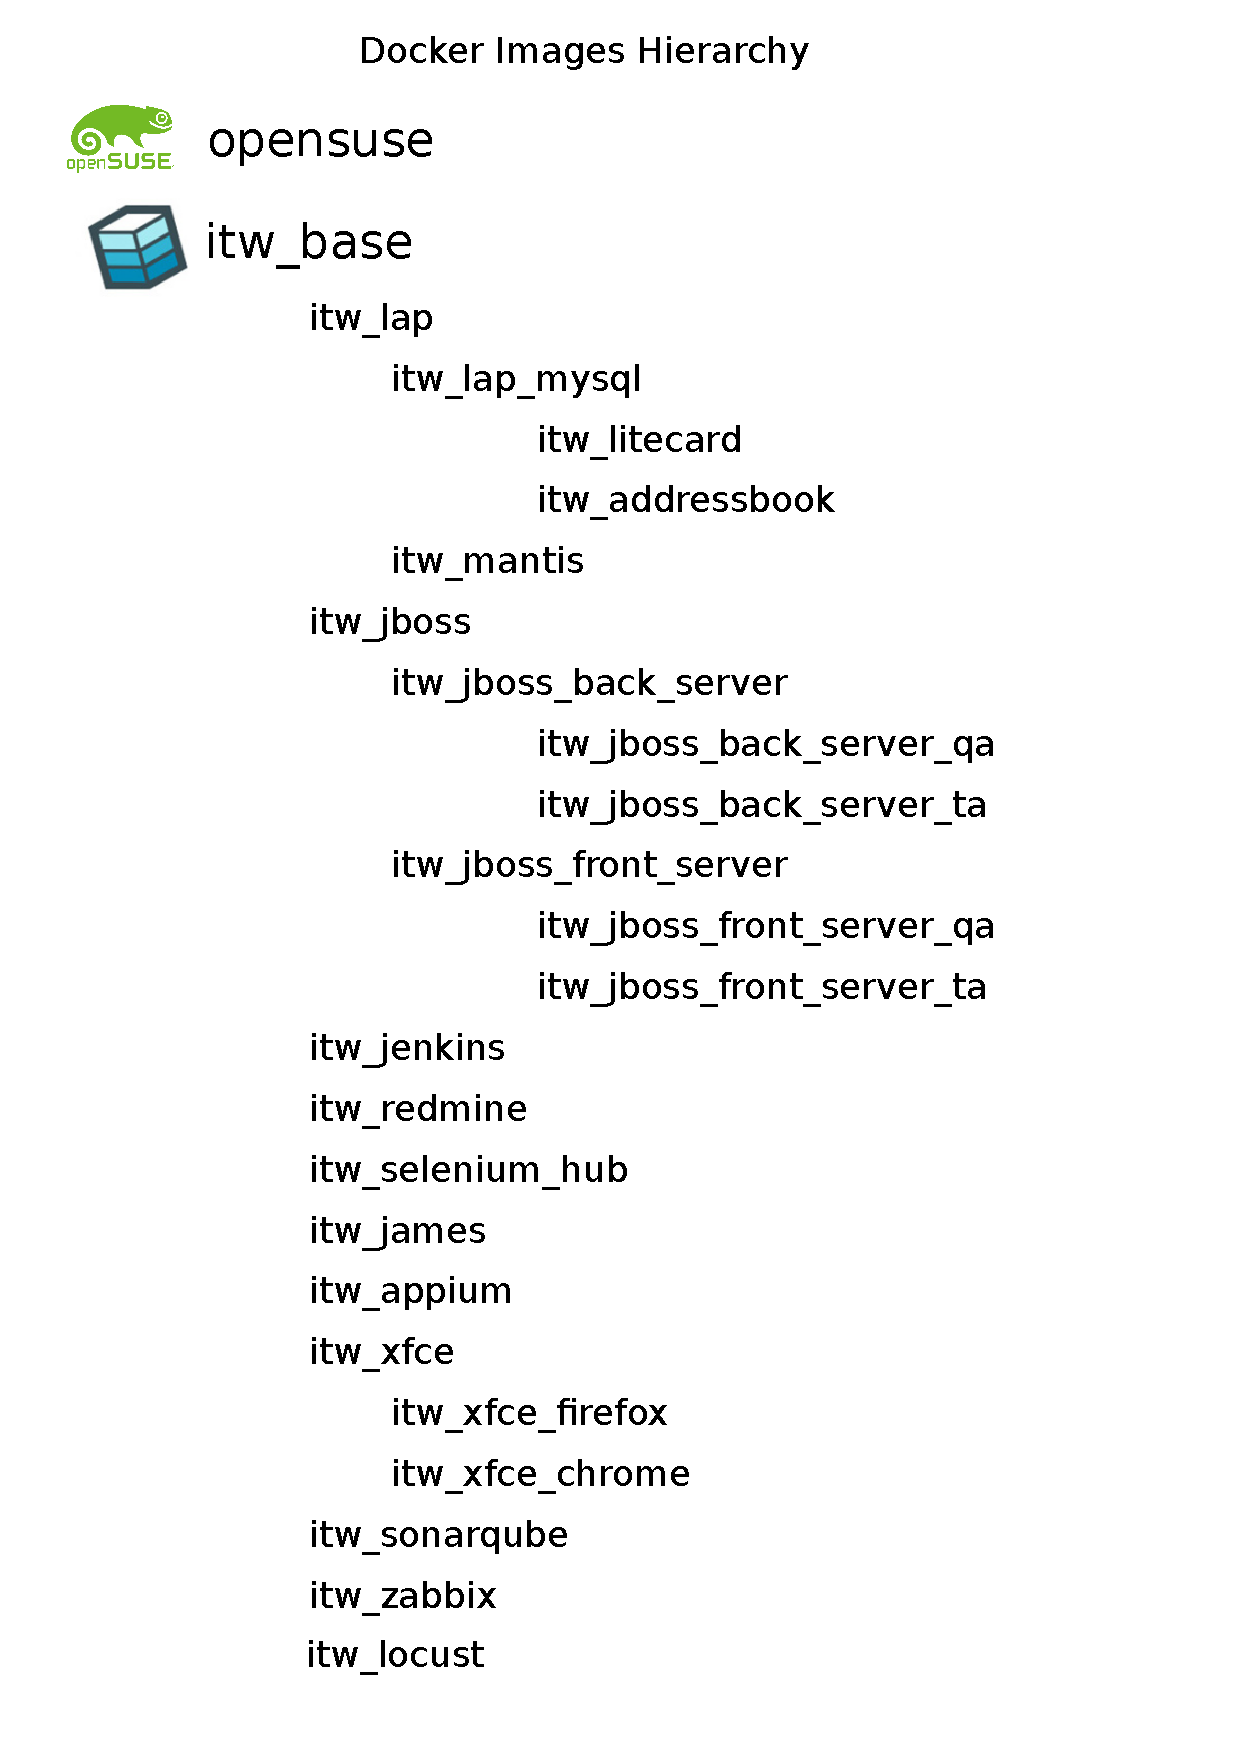
\includegraphics[width=7cm]{13_2018_Gagarin3}
  \caption{~}
  \label{Gagarin3}
\end{figure}
\end{center} 

Базовым Docker-образом является образ itw\_base. Он основан на Docker-образе OpenSUSE.

Сокращенный вариант Dockerfile с комментариями для образа itw\_base приведен по адресу \url{https://bit.ly/2LLX6j6}.

Приведенный Dockerfile не претендует на оптимальность. Его конечно можно оптимизировать, как минимум если уменьшить количество слоёв, но в рамках локальной сети это не сильно критично: все компоненты берутся из текущей папки с Dockerfile или из локальной сети.

При сборке данного образа скрипт zypper\_install\_from\_txt.sh берет построчно содержимое файла base.txt и производит установку необходимого ПО.

Сокращенное содержимое файла base.txt (то есть по сути itw\_base включает в себя перечисленное в файле ПО) можно посмотреть по адресу \url{https://bit.ly/2vvI5qW}.

Таким образом мы получаем готовый и удобный базовый образ, в котором точно есть vim, mc, сервер SSH. Одно из удобств состоит в том, что при подготовке нового образа мы можем развернуть базовый образ на рабочей машине, выполнить установку необходимого нам ПО, провести его настройку, испытания и уже затем приступить к подготовке Dockerfile на его базе.

Пример Dockerfile для дочернего образа можно посмотреть по адресу \url{https://bit.ly/2OBNZ2b}.

Все файлы Dockerfile также лежат в репозитории Mercurial. При коммите в этот репозиторий Jenkins Master начинает пересборку образов, причем он пересобирает образы только по иерархии. То есть если изменения касались промежуточного образа, то пересобираться будет промежуточный образ и его дочерние~--- другие образы затронуты не будут. Скрипт пересборки написан на Groovy и анализирует контрольную сумму в директории с файлом Dockerfile и вспомогательными файлами для сборки. Если контрольная сумма файлов в репозитории стала отличаться, то для этих образов производится пересборка. Такой подход в разы сокращает время на пересборку образов после изменений.

Если изменения коснулись образа itw\_base, то все дочерние образы пересоберутся с этим изменением.

Структура иерархии описана в файле json, пример которого можно посмотреть по адресу \url{http://bit.ly/2vbf8kq}.

\subsection*{4. Continuous Integration (CI)}

Первым делом на Gradle был написан скрипт, который собирает ядро системы. До этого ядро системы мог собрать только разработчик с помощью среды разработки. Причем чтобы собрать ядро ему нужно было прервать текущую работу,  переключить ветки репозитория таким образом, чтобы его работа не затёрлась, собрать ядро, передать его тестировщику, потом переключить ветки обратно и продолжить работу над текущей задачей.

Скрипт сборки на Gradle тестировщик может запустить в любой момент самостоятельно не прибегая к среде разработки (которая при запуске солидно жрёт память) и не отвлекать при этом разработчика.
Этот же скрипт используется для непрерывного развёртывания.

Структура CI представляет собой несколько серверов Jenkins (точнее два сервера). Каждый из них выполняет свою определённую задачу. Все они работают каждый в своём контейнере Docker.

Структура серверов Jenkins представлена на рис.~\ref{Gagarin4}:

\begin{center}
\begin{figure}[h!]
  \centering
  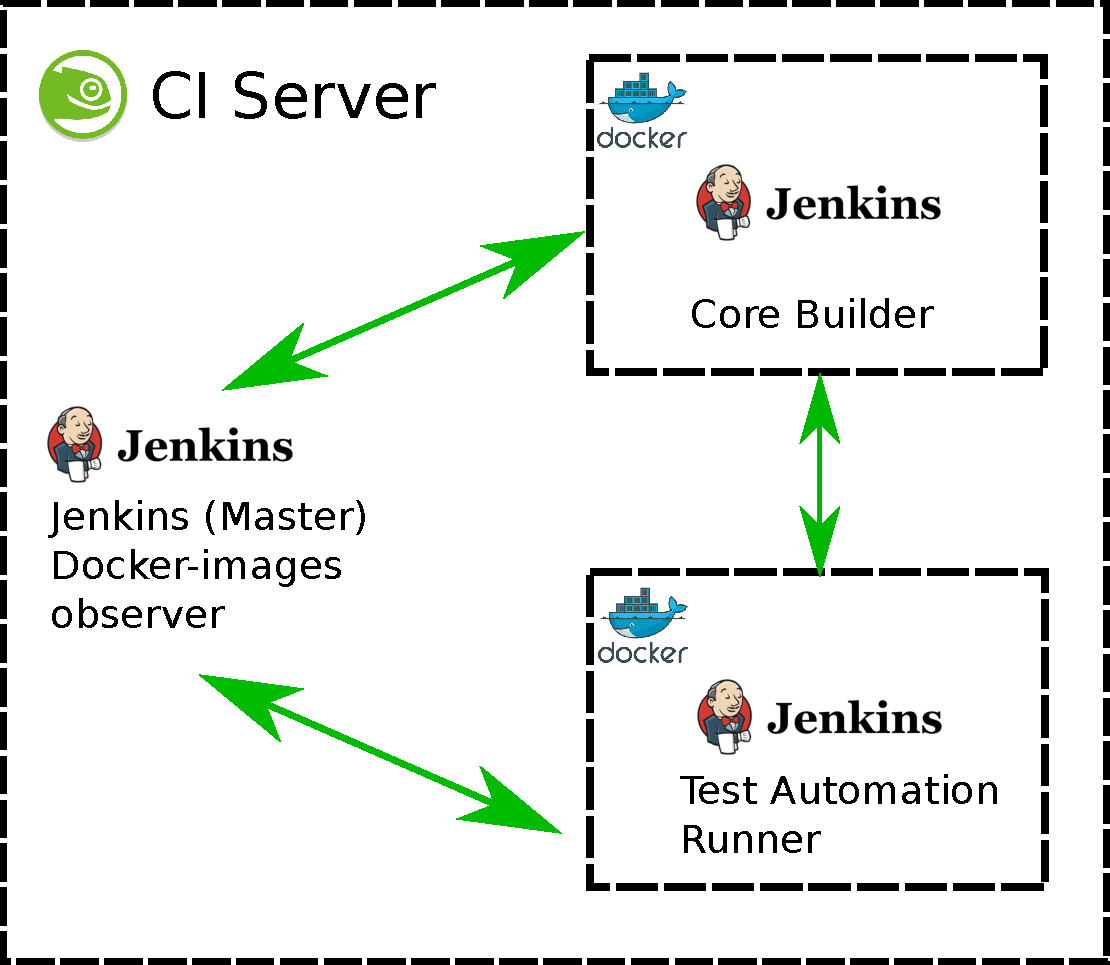
\includegraphics[width=7cm]{13_2018_Gagarin4}
  \caption{~}
  \label{Gagarin4}
\end{figure}
\end{center} 

В этой структуре сервер Jenkins Core Builder, который отвечает за сборку ядра, опрашивает репозитории с исходными кодами проекта. Когда в репозиторий в определенную ветку пришли изменения, то Jenkins производит сборку ядра, запуская скрипт Gradle для сборки.

Если сборка прошла успешно, то управление передается на\\ Jenkins Master, который из образа готовит контейнер для размещения приложения и дальнейшего его тестирования. На этом этапе также производится тестирование сборки контейнера, так как по окончании тестирования этот контейнер (уже протестированный) будет доступен тестировщику на локальной машине из реестра Docker.

Когда контейнер стартовал, то из образа в нем будет размещено и запущено приложение со всеми настройками.

После этого этапа управление передаётся на Jenkins Test\\ Automation Runner, который:

\begin{enumerate}
  \item запускает развёртывание чистой базы данных для теста;
  \item анализирует логи развёртывания базы (устанавливает все апдейты по проекту; если апдейт ошибочный, то тест будет провален);
  \item запускает JBoss сервер приложений;
  \item запускает набор <<дымовых>> браузерных тестов через Selenium Grid;
  \item анализирует логи прогона тестов;
  \item выполняет другие тестовые операции;
  \item отправляет отчет на Jenkins-инициатор.
\end{enumerate}

Результат всех выполненных шагов, также отчет Allure о прогоне тестов, рассылается в виде отчета в Jabber всем заинтересованным участникам: разработчикам, тестировщикам, инженерам DevOps.

Jenkins Test Automation Runner доступен как отдельный настроенный образ, который каждый разработчик/тестировщик может забрать себе на рабочую машину и запустить необходимый набор тестов для проверки регресса или замеров производительности.

Примерный набор тестов Jenkins TA приведён на рис.~\ref{Gagarin5}:

\begin{center}
\begin{figure}[h!]
  \centering
  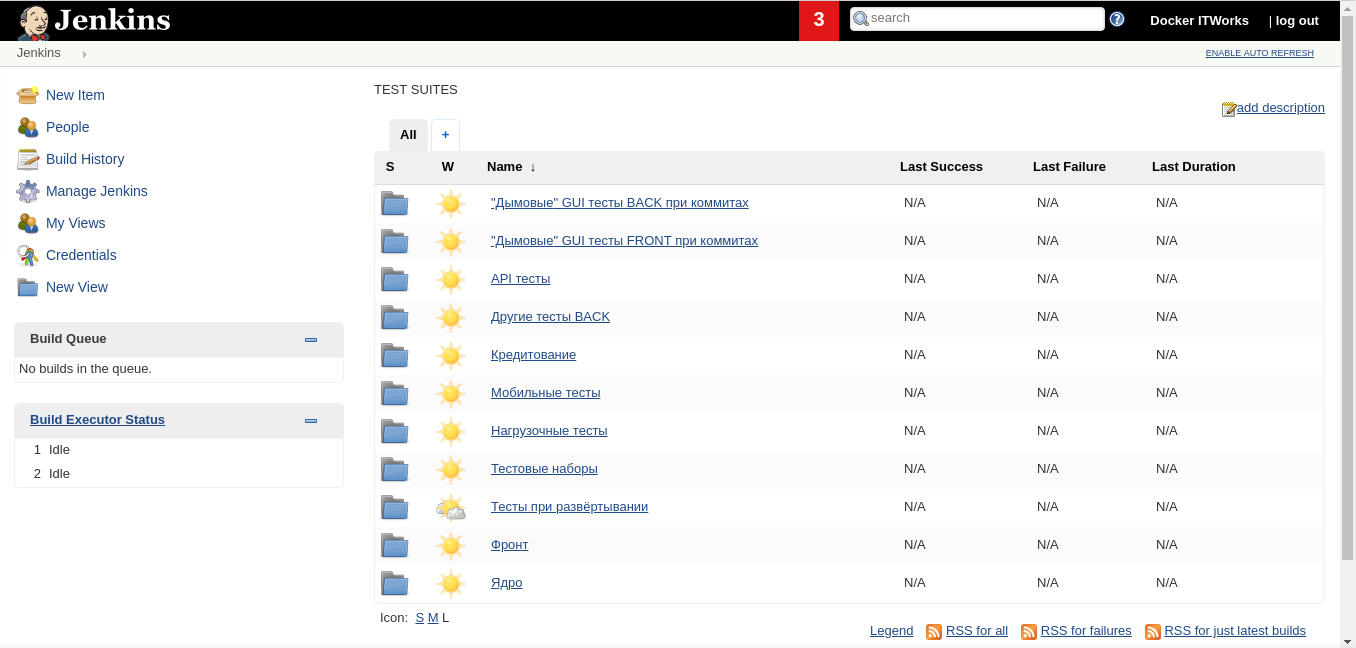
\includegraphics[width=7cm]{13_2018_Gagarin5}
  \caption{~}
  \label{Gagarin5}
\end{figure}
\end{center} 

Для обмена сообщениями между Jenkins'ами используется \\Jenkins REST API.

При коммитах, разумеется, запускается минимальный набор тестов (<<дымовые>> тесты) для получения максимально быстрой обратной связи. Но также возможен запуск и более длительных по времени регрессионных тестов. Для этих целей используются независимые сервера на CentOS из рис. 2: они не зависят от коммитов в репозиторий, и тесты на них могут выполняться несколько часов.

Результирующие отчеты Allure о тестировании помещаются на CI-сервер и доступны всем для ознакомления. Пример такого отчета можно посмотреть здесь: \url{https://demo.qameta.io/allure/latest/}.

После успешного прогона тестов Jenkins Master готовит образ Docker для специалистов по тестированию:

\begin{itemize}
  \item удаляет старый образ из реестра;
  \item собирает новый образ с приложением;
  \item размещает его в реестр образов.
\end{itemize}

Новый образ с приложением~--- полностью протестированный~--- готов для загрузки и дальнейшего использования специалистами по тестированию. Он содержит настроенный сервер со всеми артефактами, перечисленными в разделе 1 данной статьи.

В задачу QA специалиста перед началом тестирования новой доработки входит только подготовить локальную базу данных с помощью скрипта развёртывания (точно такого же, какой выполняет на шаге 1 Jenkins Test Automation Runner). Далее он просто размещает обновления от разработчика и приступает к тестированию.

\subsection*{5. Выводы}

Благодаря использованию подходов DevOps, контейнеризации, CI нам удалось существенно сократить время на регрессионное тестирование, сократить время на ручное тестирование QA"=специалистами, сократить время на подготовку тестовой среды, на выполнение других видов тестов и много других разных преимуществ, что привело к сокращению расходов заказчика и улучшению качества ПО.

Полную презентацию по докладу можно посмотреть по адресу \url{http://bit.ly/2LM4L0K}.

\end{document}

\documentclass[10pt, a5paper]{article}
\usepackage{pdfpages}
\usepackage{parallel}
\usepackage[T2A]{fontenc}
\usepackage{ucs}
\usepackage[utf8x]{inputenc}
\usepackage[polish,english,russian]{babel}
\usepackage{hyperref}
\usepackage{rotating}
\usepackage[inner=2cm,top=1.8cm,outer=2cm,bottom=2.3cm,nohead]{geometry}
\usepackage{listings}
\usepackage{graphicx}
\usepackage{wrapfig}
\usepackage{longtable}
\usepackage{indentfirst}
\usepackage{array}
\newcolumntype{P}[1]{>{\raggedright\arraybackslash}p{#1}}
\frenchspacing
\usepackage{fixltx2e} %text sub- and superscripts
\usepackage{icomma} % коскі ў матэматычным рэжыме
\PreloadUnicodePage{4}

\newcommand{\longpage}{\enlargethispage{\baselineskip}}
\newcommand{\shortpage}{\enlargethispage{-\baselineskip}}

\def\switchlang#1{\expandafter\csname switchlang#1\endcsname}
\def\switchlangbe{
\let\saverefname=\refname%
\def\refname{Літаратура}%
\def\figurename{Іл.}%
}
\def\switchlangen{
\let\saverefname=\refname%
\def\refname{References}%
\def\figurename{Fig.}%
}
\def\switchlangru{
\let\saverefname=\refname%
\let\savefigurename=\figurename%
\def\refname{Литература}%
\def\figurename{Рис.}%
}

\hyphenation{admi-ni-stra-tive}
\hyphenation{ex-pe-ri-ence}
\hyphenation{fle-xi-bi-li-ty}
\hyphenation{Py-thon}
\hyphenation{ma-the-ma-ti-cal}
\hyphenation{re-ported}
\hyphenation{imp-le-menta-tions}
\hyphenation{pro-vides}
\hyphenation{en-gi-neering}
\hyphenation{com-pa-ti-bi-li-ty}
\hyphenation{im-pos-sible}
\hyphenation{desk-top}
\hyphenation{elec-tro-nic}
\hyphenation{com-pa-ny}
\hyphenation{de-ve-lop-ment}
\hyphenation{de-ve-loping}
\hyphenation{de-ve-lop}
\hyphenation{da-ta-ba-se}
\hyphenation{plat-forms}
\hyphenation{or-ga-ni-za-tion}
\hyphenation{pro-gramming}
\hyphenation{in-stru-ments}
\hyphenation{Li-nux}
\hyphenation{sour-ce}
\hyphenation{en-vi-ron-ment}
\hyphenation{Te-le-pathy}
\hyphenation{Li-nux-ov-ka}
\hyphenation{Open-BSD}
\hyphenation{Free-BSD}
\hyphenation{men-ti-on-ed}
\hyphenation{app-li-ca-tion}

\def\progref!#1!{\texttt{#1}}
\renewcommand{\arraystretch}{2} %Іначай формулы ў матрыцы зліпаюцца з лініямі
\usepackage{array}

\def\interview #1 (#2), #3, #4, #5\par{

\section[#1, #3, #4]{#1 -- #3, #4}
\def\qname{LVEE}
\def\aname{#1}
\def\q ##1\par{{\noindent \bf \qname: ##1 }\par}
\def\a{{\noindent \bf \aname: } \def\qname{L}\def\aname{#2}}
}

\def\interview* #1 (#2), #3, #4, #5\par{

\section*{#1\\{\small\rm #3, #4. #5}}

\def\qname{LVEE}
\def\aname{#1}
\def\q ##1\par{{\noindent \bf \qname: ##1 }\par}
\def\a{{\noindent \bf \aname: } \def\qname{L}\def\aname{#2}}
}

\begin{document}
\title{Альт на Эльбрусе: обе вершины\footnote{\url{mike@altlinux.org}, \url{https://lvee.org/en/abstracts/286}}}
\author{Михаил Шигорин, Москва, Russian Federation}
\maketitle
\begin{abstract}
Elbrus 801-PC workstation supports three displays out-of-box but is further extendable to dual-seat configuration (with each seat still supporting up to three displays); that's what we've done in ALT installer.
\end{abstract}
Рабочая станция <<Эльбрус 801-РС(e801)>>~\cite{Shigorin-1} идёт в комплекте с трёхголовой видеокартой, а если добавить ещё одну такую же~--- возможно разместить на одной машине два полноценных рабочих места: ресурсов для них более чем достаточно (8 ядер, 32 Гб ОЗУ), а вот экономический эффект получается кратный.

Мы решили опробовать <<многоголовый>> вариант этой весной в рамках подготовки к конференции OS Day~\cite{Shigorin-2} 2018; сперва воспользовались свободными выходами уже имеющейся видеокарты, но такая конфигурация с промежуточной прослойкой Xephyr получилась небыстрой из-за отсутствия 3D-ускорения (у нас уже MATE 1.20, собранный с GTK+3), плюс достаточно громоздкой и неудобной в настройке и запуске (хотя по факту и она тоже возможна)~--- а вот с раздельными видеокартами всё стало простым и лаконичным, на данном этапе даже не потребовалось ничего патчить.

Описаны разные варианты~\cite{Shigorin-3}~\cite{Shigorin-4}~\cite{Shigorin-5} ~--- с одинаковыми или различными GPU, с задействованием logind или без него; с учётом особенностей платформы и своих предпочтений  остановились на двух Radeon R5 230 (один штатный и один дополнительный во втором слоте PCIe x8) и wdm~\cite{Shigorin-6}, который умеет поднимать несколько X-серверов штатным образом.

Реализация упакована в составе пакета xorg-conf-e801-dualseat~\cite{Shigorin-7} и вместе с доработкой инсталятора дистрибутива Альт Рабочая станция~\cite{Shigorin-8} для Эльбруса попала в августовский выпуск <<репозитория>> и образов(доступны клиентам МЦСТ)~\cite{Shigorin-9}~--- так что обладатели рабочих станций <<Эльбрус 801-РС>> могут уже сейчас обратиться в МЦСТ для получения дистрибутива и его развёртывания.

\begin{thebibliography}{20}

\bibitem{Shigorin-1} Эльбрус 801-РС \url{http://www.mcst.ru/elbrus_801-pc}
\bibitem{Shigorin-2} OS Day \url{http://osday.ru}
\bibitem{Shigorin-3} Ныне покойная multiseat wiki \url{http://web.archive.org/web/20101030044616/http://wiki.c3sl.ufpr.br/multiseat/index.php/Main_Page}
\bibitem{Shigorin-4} Multiseat in Gentoo Wiki \url{https://wiki.gentoo.org/wiki/Multiseat}
\bibitem{Shigorin-5} Multiseat in Arch Wiki \url{https://wiki.archlinux.org/index.php/xorg_multiseat}
\bibitem{Shigorin-6} wdm \url{http://altlinux.org/X11/DualSeat}
\bibitem{Shigorin-7} xorg-conf-e801-dualseat \url{http://git.altlinux.org/people/mike/packages/?p=xorg-conf-e801-dualseat.git}
\bibitem{Shigorin-8} Альт Рабочая станция \url{http://basealt.ru/products/alt-workstation/}
\bibitem{Shigorin-9} Репозиторий и образы \url{http://altlinux.org/ports/e2k}
\end{thebibliography}
\end{document}

\documentclass[10pt, a5paper]{article}
\usepackage{pdfpages}
\usepackage{parallel}
\usepackage[T2A]{fontenc}
\usepackage{ucs}
\usepackage[utf8x]{inputenc}
\usepackage[polish,english,russian]{babel}
\usepackage{hyperref}
\usepackage{rotating}
\usepackage[inner=2cm,top=1.8cm,outer=2cm,bottom=2.3cm,nohead]{geometry}
\usepackage{listings}
\usepackage{graphicx}
\usepackage{wrapfig}
\usepackage{longtable}
\usepackage{indentfirst}
\usepackage{array}
\newcolumntype{P}[1]{>{\raggedright\arraybackslash}p{#1}}
\frenchspacing
\usepackage{fixltx2e} %text sub- and superscripts
\usepackage{icomma} % коскі ў матэматычным рэжыме
\PreloadUnicodePage{4}

\newcommand{\longpage}{\enlargethispage{\baselineskip}}
\newcommand{\shortpage}{\enlargethispage{-\baselineskip}}

\def\switchlang#1{\expandafter\csname switchlang#1\endcsname}
\def\switchlangbe{
\let\saverefname=\refname%
\def\refname{Літаратура}%
\def\figurename{Іл.}%
}
\def\switchlangen{
\let\saverefname=\refname%
\def\refname{References}%
\def\figurename{Fig.}%
}
\def\switchlangru{
\let\saverefname=\refname%
\let\savefigurename=\figurename%
\def\refname{Литература}%
\def\figurename{Рис.}%
}

\hyphenation{admi-ni-stra-tive}
\hyphenation{ex-pe-ri-ence}
\hyphenation{fle-xi-bi-li-ty}
\hyphenation{Py-thon}
\hyphenation{ma-the-ma-ti-cal}
\hyphenation{re-ported}
\hyphenation{imp-le-menta-tions}
\hyphenation{pro-vides}
\hyphenation{en-gi-neering}
\hyphenation{com-pa-ti-bi-li-ty}
\hyphenation{im-pos-sible}
\hyphenation{desk-top}
\hyphenation{elec-tro-nic}
\hyphenation{com-pa-ny}
\hyphenation{de-ve-lop-ment}
\hyphenation{de-ve-loping}
\hyphenation{de-ve-lop}
\hyphenation{da-ta-ba-se}
\hyphenation{plat-forms}
\hyphenation{or-ga-ni-za-tion}
\hyphenation{pro-gramming}
\hyphenation{in-stru-ments}
\hyphenation{Li-nux}
\hyphenation{sour-ce}
\hyphenation{en-vi-ron-ment}
\hyphenation{Te-le-pathy}
\hyphenation{Li-nux-ov-ka}
\hyphenation{Open-BSD}
\hyphenation{Free-BSD}
\hyphenation{men-ti-on-ed}
\hyphenation{app-li-ca-tion}

\def\progref!#1!{\texttt{#1}}
\renewcommand{\arraystretch}{2} %Іначай формулы ў матрыцы зліпаюцца з лініямі
\usepackage{array}

\def\interview #1 (#2), #3, #4, #5\par{

\section[#1, #3, #4]{#1 -- #3, #4}
\def\qname{LVEE}
\def\aname{#1}
\def\q ##1\par{{\noindent \bf \qname: ##1 }\par}
\def\a{{\noindent \bf \aname: } \def\qname{L}\def\aname{#2}}
}

\def\interview* #1 (#2), #3, #4, #5\par{

\section*{#1\\{\small\rm #3, #4. #5}}

\def\qname{LVEE}
\def\aname{#1}
\def\q ##1\par{{\noindent \bf \qname: ##1 }\par}
\def\a{{\noindent \bf \aname: } \def\qname{L}\def\aname{#2}}
}

%\switchlang{ru}
\begin{document}
\title{Свободное программное обеспечение в образовательном учреждении Сергиево-Посадский филиал ВГИК им. С.А. Герасимова\footnote{\url{grishkin@mail.ru}, \url{https://lvee.org/en/abstracts/287}}}
\author{А.В. Гришкин, г. Сергиев Посад,  Россия, \\ А.А. Маркина, г. Брест, Республика Беларусь}
\maketitle
\begin{abstract}
The questions of the use of free software are considered both in the process of preparing the student and in the form of a means of supporting the educational process (educational environment) in the Sergiev Posad branch of the All-Russian State Institute of Cinematography. S.A. Gerasimov (VGIK). An overview is given of the free software used to organize a single information and educational environment for the institution to implement the requirements of the current legislation in the Russian Federation in the implementation of training programs for specialists in secondary vocational education and higher education.
\end{abstract}
В 2018 Сергиево-Посадскому филиалу Всероссийского\linebreak Государственного Института кинематографии им. С.А. Герасимова году исполнилось 70 лет. Учебное заведение много лет реализовывало программы среднего профессионального образования. В 2011 году, после присоединения к ВГИК, в филиале возникла необходимость реализации программ высшего образования.

Программное обеспечение, используемое в филиале, можно разделить на две категории: средства поддеркжи учебного процесса и изучаемые программные системы.

\subsection*{Средства поддержки учебного процесса}

Начиная с федеральных государственных образовательных стандартов (ФГОС) третьего поколения, при реализации программ высшего образования, обязательным является наличие в образовательной организации единой информационно-образовательной среды\linebreak (ЕИОС).

ФГОС выдвигает следующие цели использования ЕИОС при реализации программ высшего образования:

\begin{itemize}
  \item доступ к учебным планам, рабочим программам дисциплин (модулей), практик, к изданиям электронных библиотечных систем и электронным образовательным ресурсам, указанным в рабочих программах;
  \item фиксацию хода образовательного процесса, результатов промежуточной аттестации и результатов освоения основной образовательной программы;
  \item проведение всех видов занятий, процедур оценки результатов обучения, реализация которых предусмотрена с применением электронного обучения, дистанционных образовательных технологий;
  \item формирование электронного портфолио обучающегося, в том числе сохранение работ обучающегося, рецензий и оценок на эти работы со стороны любых участников образовательного процесса;
  \item взаимодействие между участниками образовательного процесса, в том числе синхронное и (или) асинхронное взаимодействия посредством сети <<Интернет>>.
\end{itemize}

Функционирование электронной информационно-\linebreak образовательной среды обеспечивается соответствующими средствами информационно-коммуникационных технологий и квалификацией работников, ее использующих и поддерживающих. Функционирование электронной информационно-образовательной среды\linebreak должно соответствовать законодательству Российской Федерации. Т.е. при организации ЕИОС необходимо обеспечить соблюдение Федеральный закон от 27 июля 2006 г. N 149-ФЗ <<Об информации, информационных технологиях и о защите информации>> и Федеральный закон от 27 июля 2006 г. N 152-ФЗ <<О персональных данных>> (Собрание законодательства Российской Федерации. (п.7.1.2. стандарта).

При обеспечении доступа к учебным планам, рабочим программам дисциплин (модулей), практик, к изданиям электронных библиотечных систем и электронным образовательным ресурсам, указанным в рабочих программах следует учесть, что аналогичные требования по доступу к перечисленным документам также установлены Постановлением Правительства РФ от 10.07.2013 N 582 (ред. от 07.08.2017) "Об утверждении Правил размещения на официальном сайте образовательной организации в информационно-телекоммуникационной сети <<Интернет>> и обновления информации об образовательной организации". Т.о. для однократности размещения и минимизации ошибок при обновлении, частью ЕИОС можно считать официальный сайт учебного учреждения.

Организация сайта учебного учреждения регламентируется приказом Рособрнадзора от 29.05.2014 N 785 <<Об утверждении требований к структуре официального сайта образовательной организации в информационно-телекоммуникационной сети <<Интернет>> и формату представления на нем информации>> (Зарегистрировано в Минюсте России 04.08.2014 N 33423). Приказ устанавливает не только перечень, наименование, адрес и минимальное содержание разделов, но и требования к микроразметке, которая используется для выделения ключевых элементов содержания страниц и контролируется Рособрнадзором в автоматизированном режиме. Правила применения микроразметки установлены актуализированными методическими рекомендациями представления информации об образовательной организации высшего образования в открытых источниках с учетом соблюдения требований законодательства в сфере образования распространяемыми Рособрнадзором.

В Сергиево-Посадском филиале ВГИК официальный сайт построен на CMS Joomla! с доработкой отдельных модулей и реализацией автоматизированного добавления микроразметки.

Стоит отметить, что применение микроразметки позволило многим сайтам-агрегаторам в автоматическом режиме собирать информацию о учебных заведениях (например сайт ucheba.ru).

Для фиксации хода образовательного процесса, результатов промежуточной аттестации и результатов освоения основной образовательной программы, формировании электронного портфолио обучающегося, в том числе сохранение работ обучающегося, рецензий и оценок на эти работы со стороны любых участников образовательного процесса был предложено создать сайт на основе CMS Joomla! доступный исключительно внутри учебного заведения содержащий требуемую информацию. Дневным отделением для каждого обучающегося создается учетная запись с необходимыми правами доступа к материалам, по окончании обучения права доступа отбираются. В настоящее время ход образовательного процесса фиксируется скан-копиями ведомостей оценок и результатов промежуточной аттестации. В будущем планируется разработка системы хранящей структурированную информацию о успеваемости обучающихся (аналог <<электронных журналов>> для средней школы).

Остро стоит вопрос о виде и способах представления портфолио студентов с возможностью рецензий и оценок. В настоящее время результаты творческой работы студентов в филиала неструктурированно размещаются на внутреннем хранилище, при этом на специально выделенной страницы внутреннего портала размещается информация о выполненных работах. Размещение творческих работ на внешних ресурсах (Youtube, Rutube, фотохостинги) порождает проблемы соблюдения авторских и смежных прав как студентов так и владельцев материала используемого студентами.

Для проведения всех видов занятий, процедур оценки результатов обучения, реализация которых предусмотрена с применением электронного обучения, дистанционных образовательных технологий используется среда Moodle, в которой размещаются учебно-методические комплексы преподаваемых предметов (модулей). В перспективе планируется использование возможностей Moodle для проведения оценки усвоения материала предмета (модуля) как с помощью тестовых заданий, так и в результате проверки представленных студентами работ в системе.

Также на Moodle возлагается обеспечение взаимодействия между участниками образовательного процесса, но т.к. система расположена исключительно внутри филиала, доступ к ней, а следовательно и взаимодействие внутри нее, при помощи сети <<Интернет>> невозможны.

В помощь преподавателям и студентам составлен каталог библиотеки филиала в электронном виде. Система построена на базе CMS Wordpress с использованием доработанного плагина <<Book Review Library>>. Плагин регистрирует новый тип поста, определяет его таксономию и реквизиты. За отображение данных отвечает разработанная тема с разбиением объемного содержания на отдельные страницы. Сформированные описания имеющихся в библиотеке единиц полностью соответствуют стандартам оформления литературных источников для выполняемых преподавателями и студентами работ. В перспективе в электронный каталог будут включены разработанные преподавателями материалы, представленные в системе Moodle.

Формирование учебно-методического комплекса предмета (модуля) осуществляется при помощи самостоятельно разработанного на базе Node.js приложения, в качестве среды хранения в котором применяется документоориентированная база данных MongoDB.\linebreak При наполнении приложение имеет возможность получения информации из электронного каталога библиотеки филиала через\linebreak Wordpress API. Приложение позволяет сформировать рекомендуемый состав методических материалов для специальностей, курсов обучения, предметов (модулей), учитывая при этом год обучения. Основной сложностью при разработке приложения стало изменение подхода к хранению данных от реляционного к документному. Каждая запись о методическом материале хранит весь набор характеристик материала, т.о. отсутствует необходимость во время поиска формировать и использовать соединение таблиц и разные виды подзапросов.

Применение приложения позволяет агрегировать в одном месте как ссылки на описание литературы из каталога библиотеки филиала, так и ссылки на литературу в электронном виде, представленную в электронных библиотеках <<Лань>> и iBooks.ru, доступ к которым осуществляется из внутренней сети филиала.

Таким образом, можно подытожить, что применение свободного программного обеспечения в целях создания единой\linebreak информационно-образовательной среды позволяет полностью выполнить требования ФГОС, хотя и вызывает необходимость разработки дополнительного программного обеспечения. Также следует отметить, что применение ЕИОС возможно и при реализации программ среднего профессионального образования в филиале.

В перспективе в филиале ставятся задачи повышения интеграции составных частей ЕИОС между собой, более объемное применение структурированной информации, получаемой, в том числе и от внешних систем.

\subsection*{Программное обеспечение, применяемое в учебном процессе}

В настоящее время в филиале свободное программное обеспечение применяется и непосредственно в учебном процессе.

В лабораторном практикуме активно применяются:

\begin{itemize}
  \item при изучении технологий хранения данных СУБД MySQL, осуществляются первые попытки использования СУБД\linebreak MongoDB;
  \item при изучении сетевых технологий~--- сетевой анализатор\linebreak WireShark, реализации сервисов электронной почты, FTP,\linebreak DNS на базе FreeBSD или Fedora;
  \item при изучении технологий разработки программ и информационных систем~--- IDE NetBeans, Node.js, git, Notepad++, сервис draw.io.
  \item при изучении 3D моделирования, в том числе и в анимации~--- Blender3D.
\end{itemize}

\begin{thebibliography}{20}
\bibitem{Grishkin-1} Федеральный закон от 29 декабря 2012 года N 273-ФЗ <<Об образовании в Российской Федерации>> (Ст. 29).
\bibitem{Grishkin-2} Постановление Правительства Российской Федерации от 10.07.2013 N 582 <<Об утверждении Правил размещения на официальном сайте образовательной организации в информационно-телекоммуникационной сети <<Интернет>> и обновления информации об образовательной организации>>.
\bibitem{Grishkin-3} Приказ Рособрнадзора от 29.05.2014 N 785 <<Об утверждении требований к структуре официального сайта образовательной организации в информационно-телекоммуникационной сети <<Интернет>> и формату представления на нем информации>>.
\bibitem{Grishkin-4} Приказ Минобрнауки России от 16.11.2016 N 1427 <<Об утверждении федерального государственного образовательного стандарта высшего образования по специальности 55.05.01 Режиссура кино и телевидения (уровень специалитета)>> (Зарегистрировано в Минюсте России 09.12.2016 N 44634)
\end{thebibliography}

\end{document}

\documentclass[10pt, a5paper]{article}
\usepackage{pdfpages}
\usepackage{parallel}
\usepackage[T2A]{fontenc}
\usepackage{ucs}
\usepackage[utf8x]{inputenc}
\usepackage[polish,english,russian]{babel}
\usepackage{hyperref}
\usepackage{rotating}
\usepackage[inner=2cm,top=1.8cm,outer=2cm,bottom=2.3cm,nohead]{geometry}
\usepackage{listings}
\usepackage{graphicx}
\usepackage{wrapfig}
\usepackage{longtable}
\usepackage{indentfirst}
\usepackage{array}
\newcolumntype{P}[1]{>{\raggedright\arraybackslash}p{#1}}
\frenchspacing
\usepackage{fixltx2e} %text sub- and superscripts
\usepackage{icomma} % коскі ў матэматычным рэжыме
\PreloadUnicodePage{4}

\newcommand{\longpage}{\enlargethispage{\baselineskip}}
\newcommand{\shortpage}{\enlargethispage{-\baselineskip}}

\def\switchlang#1{\expandafter\csname switchlang#1\endcsname}
\def\switchlangbe{
\let\saverefname=\refname%
\def\refname{Літаратура}%
\def\figurename{Іл.}%
}
\def\switchlangen{
\let\saverefname=\refname%
\def\refname{References}%
\def\figurename{Fig.}%
}
\def\switchlangru{
\let\saverefname=\refname%
\let\savefigurename=\figurename%
\def\refname{Литература}%
\def\figurename{Рис.}%
}

\hyphenation{admi-ni-stra-tive}
\hyphenation{ex-pe-ri-ence}
\hyphenation{fle-xi-bi-li-ty}
\hyphenation{Py-thon}
\hyphenation{ma-the-ma-ti-cal}
\hyphenation{re-ported}
\hyphenation{imp-le-menta-tions}
\hyphenation{pro-vides}
\hyphenation{en-gi-neering}
\hyphenation{com-pa-ti-bi-li-ty}
\hyphenation{im-pos-sible}
\hyphenation{desk-top}
\hyphenation{elec-tro-nic}
\hyphenation{com-pa-ny}
\hyphenation{de-ve-lop-ment}
\hyphenation{de-ve-loping}
\hyphenation{de-ve-lop}
\hyphenation{da-ta-ba-se}
\hyphenation{plat-forms}
\hyphenation{or-ga-ni-za-tion}
\hyphenation{pro-gramming}
\hyphenation{in-stru-ments}
\hyphenation{Li-nux}
\hyphenation{sour-ce}
\hyphenation{en-vi-ron-ment}
\hyphenation{Te-le-pathy}
\hyphenation{Li-nux-ov-ka}
\hyphenation{Open-BSD}
\hyphenation{Free-BSD}
\hyphenation{men-ti-on-ed}
\hyphenation{app-li-ca-tion}

\def\progref!#1!{\texttt{#1}}
\renewcommand{\arraystretch}{2} %Іначай формулы ў матрыцы зліпаюцца з лініямі
\usepackage{array}

\def\interview #1 (#2), #3, #4, #5\par{

\section[#1, #3, #4]{#1 -- #3, #4}
\def\qname{LVEE}
\def\aname{#1}
\def\q ##1\par{{\noindent \bf \qname: ##1 }\par}
\def\a{{\noindent \bf \aname: } \def\qname{L}\def\aname{#2}}
}

\def\interview* #1 (#2), #3, #4, #5\par{

\section*{#1\\{\small\rm #3, #4. #5}}

\def\qname{LVEE}
\def\aname{#1}
\def\q ##1\par{{\noindent \bf \qname: ##1 }\par}
\def\a{{\noindent \bf \aname: } \def\qname{L}\def\aname{#2}}
}

\begin{document}
\title{Кластеризация систем хранения данных с помощью NFS\footnote{\url{inimicus@tut.by}, \url{https://lvee.org/en/abstracts/288}}}
\author{Влад Шарпио, Minsk, Belarus}
\maketitle
\begin{abstract}
A data storage clasterization specifics based on Parallel NFS (pNFS) is reviewed. The pNFS protocol details and architecture-related specifics are covered as well as its current state.
\end{abstract}
\section*{Кластеризация СХД}

Долгое время функция создания кластеров систем хранения данных относилось только к закрытым блочным системам. Популярность дешевых NAS  и потребность в повышенной отказоустойчивости породило цклую плеяду кластерных объектных хранилищ со сложной системой управления и еще более сложными механизмами расчета производительности. В январе  2010 было обубликована спецификация протокола NFS v4.1 RFC 5661 которая позволят использовать несколько NAS  как единое дисковое пространство.

NFS в классическом понимании состоит из серверного и клиентской частей, а тпкаже протоколов взаимодействия между ними. При работе с использованием NFS сервер скрывает реальную  структуру дисковой и файловой системы, предоставляя унифицированную среду, таким образом обеспечивая кроссплатформенное общение.

\section*{Простая конфигурация NFS}

\begin{center}
\begin{figure}[h!]
  \centering
  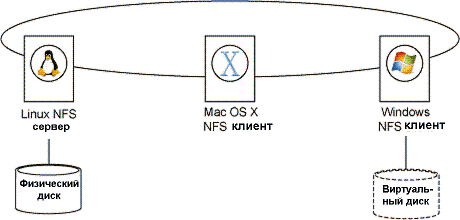
\includegraphics[width=7cm]{16_2018_Sharpio1}
  \caption{Конфигурация NFS v3}
  \label{Sharpio1}
\end{figure}
\end{center} 

Операции по фактическому чтению/записи  данных с/на дисковых или твердотельных накопителей осуществляет NFS-сервер. Вся работа с данными и метаданными возлагается  на  ресурсы сервера. Такой подход в реализации традиционно приводил к низким показателям производительности по операциям в секунду IOPS в случаях использования объектов большого размера или при случайных операциях  с большим числом объектов. Использование точечных методов в решении таких вопросов (агрегация каналов, использование быстрых файловых систем, потоковая компрессия и дедупликация) хоть и поднимало производительность отдельно взятых NAS, но всё равно  достижение уровня SAN  было практически невозможно.

По крайней мере, так было раньше.

Версия NFS 4.1 включает в себя расширение инструкций в области паралелизации работы~--- Parallel NFS (pNFS), что даёт возможность избавиться от недостатков  NFS-хранилища и обеспечить механизм повышения скорости передачи данных (за счёт обеспечения распараллеливания операций ввода/вывода).

При работе с pNFS клиенты, как и раньше, имеют доступ к файловой системе сервера, однако рабочие потоки обработки метаданных и  данных разделены. Сервер метаданных pNFS обеспечивает выполнение фазы инициализации соединения, после чего обемен данным осуществляется между клиентом и сервером NFS. Конфигурация pNFS показана на рисунке~\ref{Sharpio2}.

\begin{center}
\begin{figure}[h!]
  \centering
  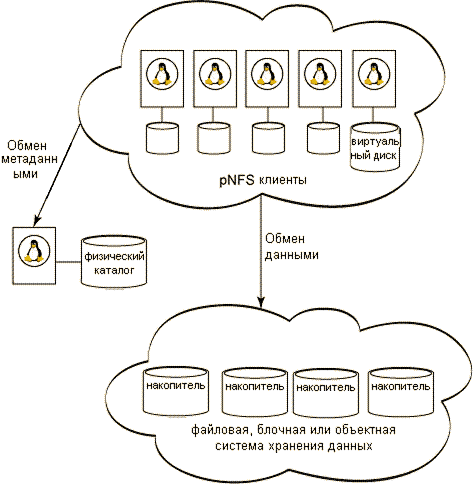
\includegraphics[width=7cm]{16_2018_Sharpio2}
  \caption{Концепция организации pNFS}
  \label{Sharpio2}
\end{figure}
\end{center} 

Задачами  сервера метаданных  является  экспорт файловой системы, хранение и поддержание каноничных метаданных. Клиент новой версии обеспечивает монтирование конечной файловой системы на основании данных pNFS сервера и обеспечивает непосредственное взаимодействие в работе с данными с NFS серверами.

Сервер pNFS не участвует в транзакциях по передаче данных, что повышает производительность.

Такой подход в работе pNFS сохраняет все удобства и преимущества NFS, добавляя к ним производительность и масштабируемость.

\section*{pNFS в деталях}

Протокол pNFS передает метаданные о объектах, в рамках единой разметки (layout), между сервером pNFS и клиентским узлом. layout описывает, как объект распределен в системе хранения данных: например, как он поделен между несколькими носителями; также в layout содержатся атрибуты файла (права доступа и т.д.). Все метаданные сохраняются в файлах разметки и хранится на сервере pNFS, а система хранения данных занимается только вводом/выводом информации.

Протокол доступа к системе хранения данных (Storage access protocol) регулирует работу клиента  с системой хранения данных. Каждый протокол доступа к системе хранения данных работает с индивидуальным layout.

Протокол управления (Control protocol) служит для синхронизации между сервером метаданных и сервером данных. Синхронизация — например, реорганизация файлов на носителях— скрыта от клиентов.

\begin{center}
\begin{figure}[h!]
  \centering
  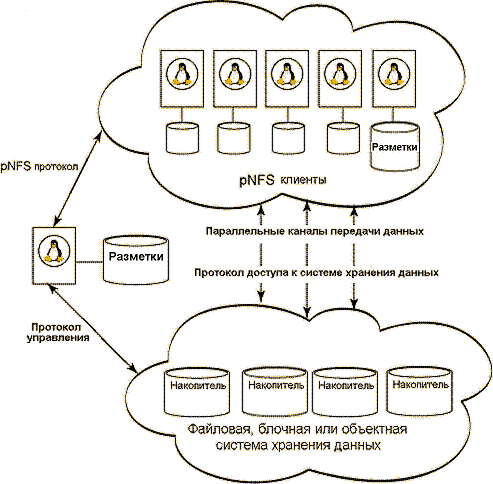
\includegraphics[width=7cm]{16_2018_Sharpio3}
  \caption{Триада протоколов pNFS}
  \label{Sharpio3}
\end{figure}
\end{center} 

Итак, процесс доступа клиента к данным выглядит так:

\begin{enumerate}
  \item Клиент запрашивает разметку файла, с которым предстоит работать.
  \item Клиент получает права доступа путем открытия файла на сервере метаданных.
  \item Авторизовавшись и получив разметку файла, клиент может получать информацию непосредственно с сервера данных. Работа осуществляется в соответствии с протоколом доступа, требуемым для этого типа носителя (подробнее ниже).
  \item Если клиент изменяет файл, клиентская копия разметки изменяется необходимым образом, после чего передается на сервер метаданных.
  \item Когда клиент больше не нуждается в файле, он записывает оставшиеся изменения, передает свою копию разметки обратно на сервер метаданных и закрывает файл.
\end{enumerate}

Более подробно операция чтения (READ) – это серия следующих операций протокола:

\begin{enumerate}
  \item Клиент посылает запрос LOOKUP+OPEN на сервер pNFS. Сервер возвращает дескриптор файла (file handle) и информацию о состоянии файла.
  \item Клиент запрашивает с сервера разметку с помощью команды LAYOUTGET. Сервер возвращает разметку файла.
  \item Клиент посылает запрос READ на устройства хранения, которые инициируют множество параллельных операций READ.
  \item Когда клиент заканчивает чтение, он посылает команду\\ LAYOUTRETURN.
  \item Если клиентская копия разметки становится неактуальной (из-за изменения серверной разметки каким-либо другим, выполняющимся параллельно действием), сервер посылает команду CB\_LAYOUTRECALL, сообщая, что разметка уже не действительна и ее надо обновить.
\end{enumerate}

Операция Write выглядит так же, за исключением того, что клиент шлет команду LAYOUTCOMMIT перед командой\\ LAYOUTRETURN, чтобы «опубликовать» свои изменения файла на сервере pNFS.

Разметки могут кэшироваться на каждом клиенте, что еще больше повышает скорость работы. Также клиент может при желании удалять свою копию разметки полученной с сервера, если она больше не используется. Также сервер позволяет ограничивать в разметке размер записываемых данных, чтобы, например, не использовать дисковые квоты или уменьшить издержки на выделение ресурсов.

Для того чтобы данные в кэше оставались актуальными, сервер метаданных отзывает устаревшие разметки. Все затронутые отзывом клиенты должны приостановить работу с данными и, либо обновить свою версию разметки, либо продолжить работу через обыкновенную NFS. Сервер обязательно делает отзыв разметки перед началом административной работы с файлом (например, миграции или изменения распределения файла по системам хранения).

Независимо от типа разметки pNFS использует для обращения к серверам общую схему. Вместо имени хоста или тома накопителя обращение к серверам происходит по уникальным идентификаторам. Этому идентификатору ставится в соответствие зависящая от конкретного протокола доступа ссылка на сервер.

Какой из этих методов хранения лучше? Ответ индивидуален и зависит от размера бюджета, масштаба системы, требуемой скорости, простоты работы и других факторов.

\section*{Текущее состояние pNFS}

Нативная поддержка протокола на уровне ядра доступна с версий
2.6.37, поддержка всего функционала полностью реализована в ветке 3.1.

Мейнтейнером развития является коммерческая организация \\Panasas,  активная часть сообщества~--- 118 аккаунтов.

Основная ветка развития протокола 4.1 завершена в 2010 году.
С 2014 и по настоящее время идёт стандартизация (формально завершена в 2016) и развитие  ветки 4.2.

\begin{thebibliography}{20}
  \bibitem{Sharpio-1} \url{https://www.snia.org/sites/default/files/NFS\_4.2\_Final.pdf}
  \bibitem{Sharpio-2} \url{http://linux-nfs.org}
  \bibitem{Sharpio-3} \url{https://www.ibm.com/developerworks/ru/library/l-pnfs}
  \bibitem{Sharpio-4} \url{https://tools.ietf.org/html/rfc7862}
  \bibitem{Sharpio-5} \url{https://tools.ietf.org/html/rfc5661}
\end{thebibliography}

\end{document}

\documentclass[10pt, a5paper]{article}
\usepackage{pdfpages}
\usepackage{parallel}
\usepackage[T2A]{fontenc}
\usepackage{ucs}
\usepackage[utf8x]{inputenc}
\usepackage[polish,english,russian]{babel}
\usepackage{hyperref}
\usepackage{rotating}
\usepackage[inner=2cm,top=1.8cm,outer=2cm,bottom=2.3cm,nohead]{geometry}
\usepackage{listings}
\usepackage{graphicx}
\usepackage{wrapfig}
\usepackage{longtable}
\usepackage{indentfirst}
\usepackage{array}
\newcolumntype{P}[1]{>{\raggedright\arraybackslash}p{#1}}
\frenchspacing
\usepackage{fixltx2e} %text sub- and superscripts
\usepackage{icomma} % коскі ў матэматычным рэжыме
\PreloadUnicodePage{4}

\newcommand{\longpage}{\enlargethispage{\baselineskip}}
\newcommand{\shortpage}{\enlargethispage{-\baselineskip}}

\def\switchlang#1{\expandafter\csname switchlang#1\endcsname}
\def\switchlangbe{
\let\saverefname=\refname%
\def\refname{Літаратура}%
\def\figurename{Іл.}%
}
\def\switchlangen{
\let\saverefname=\refname%
\def\refname{References}%
\def\figurename{Fig.}%
}
\def\switchlangru{
\let\saverefname=\refname%
\let\savefigurename=\figurename%
\def\refname{Литература}%
\def\figurename{Рис.}%
}

\hyphenation{admi-ni-stra-tive}
\hyphenation{ex-pe-ri-ence}
\hyphenation{fle-xi-bi-li-ty}
\hyphenation{Py-thon}
\hyphenation{ma-the-ma-ti-cal}
\hyphenation{re-ported}
\hyphenation{imp-le-menta-tions}
\hyphenation{pro-vides}
\hyphenation{en-gi-neering}
\hyphenation{com-pa-ti-bi-li-ty}
\hyphenation{im-pos-sible}
\hyphenation{desk-top}
\hyphenation{elec-tro-nic}
\hyphenation{com-pa-ny}
\hyphenation{de-ve-lop-ment}
\hyphenation{de-ve-loping}
\hyphenation{de-ve-lop}
\hyphenation{da-ta-ba-se}
\hyphenation{plat-forms}
\hyphenation{or-ga-ni-za-tion}
\hyphenation{pro-gramming}
\hyphenation{in-stru-ments}
\hyphenation{Li-nux}
\hyphenation{sour-ce}
\hyphenation{en-vi-ron-ment}
\hyphenation{Te-le-pathy}
\hyphenation{Li-nux-ov-ka}
\hyphenation{Open-BSD}
\hyphenation{Free-BSD}
\hyphenation{men-ti-on-ed}
\hyphenation{app-li-ca-tion}

\def\progref!#1!{\texttt{#1}}
\renewcommand{\arraystretch}{2} %Іначай формулы ў матрыцы зліпаюцца з лініямі
\usepackage{array}

\def\interview #1 (#2), #3, #4, #5\par{

\section[#1, #3, #4]{#1 -- #3, #4}
\def\qname{LVEE}
\def\aname{#1}
\def\q ##1\par{{\noindent \bf \qname: ##1 }\par}
\def\a{{\noindent \bf \aname: } \def\qname{L}\def\aname{#2}}
}

\def\interview* #1 (#2), #3, #4, #5\par{

\section*{#1\\{\small\rm #3, #4. #5}}

\def\qname{LVEE}
\def\aname{#1}
\def\q ##1\par{{\noindent \bf \qname: ##1 }\par}
\def\a{{\noindent \bf \aname: } \def\qname{L}\def\aname{#2}}
}

\begin{document}
\title{OSTree~--- атомарные обновления ОС в стиле git\footnote{\url{d4s@t-linux.by}, \url{https://lvee.org/en/abstracts/289}}}
\author{Denis Pynkin, Minsk, Belarus}
\maketitle
\begin{abstract}
LibOSTree (aka "OSTree") project is aimed to create git-like bootable filesystem trees.
This is shared library and set of utilities to manage content-addressed-object store
and local "checkouts" of filesystem trees allowing transactional upgrades and rollbacks of the system.
\end{abstract}

\section*{Что такое OSTree}

OSTree\footnote{\url{https://ostree.readthedocs.io}} предназначен для создания неизменяемых файловых систем в стиле git, обеспечивая атомарные обновления и откаты ОС. Проект предоставляет собой референсную библиотеку для работы с репозиториями <<ostree>>, а также утилиту командной строки, позволяющей производить все необходимые операции над локальным репозиторием.

В локальном <<ostree>> репозитории хранятся <<снимки>> файлов и директорий, позволяя быстро переключать корневую систему, ядро и конфигурацию загрузчика на любой из доступных вариантов.

Серверный репозиторий предназначен для использования в качестве источника обновлений поверх HTTP/HTTPS протокола. Возможность использования GPG-подписи отдельных коммитов, а также внутренняя архитектура репозитория, позволяют тиражировать серверный репозиторий и использовать его для обновлений даже из недоверенных источников.

\section*{Локальная архитектура OSTree}

OSTree предназначен для работы поверх любой POSIX-\linebreak совместимой файловой системы.

В репозитории <</ostree/repo>> хранятся файловые объекты, а также ссылки на них~--- в этом репозиторий <<ostree>> очень похож на репозиторий <<git>>. Имена всех объектов в системе представляют собой sha256 хэш от содержимого, таким образом обеспечивается автоматическая дедупликация данных на уровне репозитория.

В репозитории присутствуют 3 базовых типа файлов:

\begin{itemize}
  \item <sha256>.commit~--- описание коммита, а также <<имя>> корневой директории
  \item <sha256>.dirtree~--- список файловых объектов в директории
  \item <sha256>.file~--- файл
\end{itemize}

В отличие от git, при разворачивании (checkout, deploy) все файлы создаются в виде жёсткой ссылки на изначальный файл, находящийся в репозитории, что накладывает серьёзное ограничение~--- репозиторий и развёрнутый корень системы обязаны находится на одной ФС.

Директорий <</ostree/deploy>> хранит развернутые корневые файловые системы в поддиректории, соответствующей имени операционной системы. Да, OSTree позволяет устанавливать и переключаться между несколькими разными, не связанными между собой ОС!

В концепции OSTree предполагается, что только 2 системные директории <</etc>> и <</var>> остаются в режиме записи, причем <</etc>> копируется (3-way merge) при переключении, а <</var>> --- является общей в рамках одной ОС.

Таких развернутых версий разных ОС (stateroot) одновременно может быть несколько.

\section*{Загрузка системы}

При разворачивании корня ОС, как правило копируется ядро и initrd, поставляемые с этой версией, а также создается новая конфигурация загрузчика. До того момента, пока конфигурация загрузчика не <<переключится>> с помощью атомарной операции создания символической ссылки на обновленную конфигурацию, загрузка системы будет осуществляться в текущую версию ОС. Поэтому при обновлении системы данная операция осуществляется в последнюю очередь. В любой момент времени ОС будет в состоянии загрузиться либо в <<текущую>> версию, либо в <<обновленную>>.

Загрузка ОС, адаптированной для OSTree предполагает, что решение, какая ОС и её версия будут загружаться, принимается на этапе работы <<минисистемы>> в initrd, поскольку для создания загрузочной корневой системы необходимо <<правильно>> подмонтировать все её части. Из-за этого невозможно применять OSTree без initrd.

Версия ОС для загрузки, как правило передается с помощью опции командной строки для ядра <<ostree=>>, содржащей полный путь к развернутому корню операционной системы, например:

\begin{verbatim}
`ostree=/ostree/boot.1/apertis/0082844f3f7223ea5093f6c25
0f50a35c83a5bfe2e96799bc94c3e3be95a60a0/0`\end{verbatim}
Данный параметр генерируется, как часть конфигурации загрузчика на этапе разворачивания корневой ФС.

В отличие от <<классических>> ОС, которым достаточно правильно инициализировать блочное устройство, для OSTree необходимо дополнительно подмонтировать все корневые директории перед вызовом <<pivot\_root>>. Референсный пример <<switchroot.sh>> доступен в git-репозитории OSTree\footnote{\url{https://github.com/ostreedev/ostree/tree/master/src/switchroot}}.

\section*{Использование в Apertis}

Для адаптации ОС, основанной на Debian, к работе с OSTree потребовалось:

\begin{itemize}
  \item доработать OSTree для корректного взаимодействия с загрузчиком <<u-boot>>;
  \item обеспечить загрузку и работу ОС в режиме R/O для корневой файловой системы;
  \item фактически создать собственную сборочную систему на базе Debos;
  \item переписать тесты, требующие установки дополнительных пакетов.
\end{itemize}

Кроме того для внутренних нужд был разработан шаблон\footnote{\url{https://gitlab.apertis.org/infrastructure/apertis-image-recipes/tree/master/lxc}} для работы системы на основе OSTree в качестве контейнера LXC, что позволяет быстро и безопасно эксперементировать с технологией.

\end{document}

\documentclass[10pt, a5paper]{article}
\usepackage{pdfpages}
\usepackage{parallel}
\usepackage[T2A]{fontenc}
\usepackage{ucs}
\usepackage[utf8x]{inputenc}
\usepackage[polish,english,russian]{babel}
\usepackage{hyperref}
\usepackage{rotating}
\usepackage[inner=2cm,top=1.8cm,outer=2cm,bottom=2.3cm,nohead]{geometry}
\usepackage{listings}
\usepackage{graphicx}
\usepackage{wrapfig}
\usepackage{longtable}
\usepackage{indentfirst}
\usepackage{array}
\newcolumntype{P}[1]{>{\raggedright\arraybackslash}p{#1}}
\frenchspacing
\usepackage{fixltx2e} %text sub- and superscripts
\usepackage{icomma} % коскі ў матэматычным рэжыме
\PreloadUnicodePage{4}

\newcommand{\longpage}{\enlargethispage{\baselineskip}}
\newcommand{\shortpage}{\enlargethispage{-\baselineskip}}

\def\switchlang#1{\expandafter\csname switchlang#1\endcsname}
\def\switchlangbe{
\let\saverefname=\refname%
\def\refname{Літаратура}%
\def\figurename{Іл.}%
}
\def\switchlangen{
\let\saverefname=\refname%
\def\refname{References}%
\def\figurename{Fig.}%
}
\def\switchlangru{
\let\saverefname=\refname%
\let\savefigurename=\figurename%
\def\refname{Литература}%
\def\figurename{Рис.}%
}

\hyphenation{admi-ni-stra-tive}
\hyphenation{ex-pe-ri-ence}
\hyphenation{fle-xi-bi-li-ty}
\hyphenation{Py-thon}
\hyphenation{ma-the-ma-ti-cal}
\hyphenation{re-ported}
\hyphenation{imp-le-menta-tions}
\hyphenation{pro-vides}
\hyphenation{en-gi-neering}
\hyphenation{com-pa-ti-bi-li-ty}
\hyphenation{im-pos-sible}
\hyphenation{desk-top}
\hyphenation{elec-tro-nic}
\hyphenation{com-pa-ny}
\hyphenation{de-ve-lop-ment}
\hyphenation{de-ve-loping}
\hyphenation{de-ve-lop}
\hyphenation{da-ta-ba-se}
\hyphenation{plat-forms}
\hyphenation{or-ga-ni-za-tion}
\hyphenation{pro-gramming}
\hyphenation{in-stru-ments}
\hyphenation{Li-nux}
\hyphenation{sour-ce}
\hyphenation{en-vi-ron-ment}
\hyphenation{Te-le-pathy}
\hyphenation{Li-nux-ov-ka}
\hyphenation{Open-BSD}
\hyphenation{Free-BSD}
\hyphenation{men-ti-on-ed}
\hyphenation{app-li-ca-tion}

\def\progref!#1!{\texttt{#1}}
\renewcommand{\arraystretch}{2} %Іначай формулы ў матрыцы зліпаюцца з лініямі
\usepackage{array}

\def\interview #1 (#2), #3, #4, #5\par{

\section[#1, #3, #4]{#1 -- #3, #4}
\def\qname{LVEE}
\def\aname{#1}
\def\q ##1\par{{\noindent \bf \qname: ##1 }\par}
\def\a{{\noindent \bf \aname: } \def\qname{L}\def\aname{#2}}
}

\def\interview* #1 (#2), #3, #4, #5\par{

\section*{#1\\{\small\rm #3, #4. #5}}

\def\qname{LVEE}
\def\aname{#1}
\def\q ##1\par{{\noindent \bf \qname: ##1 }\par}
\def\a{{\noindent \bf \aname: } \def\qname{L}\def\aname{#2}}
}

\begin{document}
\title{Юридические вопросы по раскрытию  программного кода в общий доступ\footnote{\url{mike@altlinux.org}, \url{https://lvee.org/en/abstracts/291}}}
\author{Дeнис Дoротенко, юрисконсульт ООО <<ЯНДЕКС>>}
\maketitle
\begin{abstract}
This material is intended to describe the legal side of developing software and releasing its source code in public access. Such aspects as third party components licensing compliance, copyright and trademark rights infringements, contribution license agreements, authorship notices are covered by this text.
Keywords: open source, licensing compliance, CLA, copyright, Yandex.
Author: Denis Dorotenko, Legal Counsel at Yandex LLC (\url{http://yandex.ru}). Among other work duties, he is responsible for legal support of Yandex own open source projects (\url{https://github.com/yandex/}).
\end{abstract}

\section*{Позиция компании Яндекс может не совпадать с позицией автора.}

В настоящее время все также можно встретить дискуссии о том, является ли бизнес-модель открытого программного обеспечения успешной.  В любом случае, нам известны достаточно успешные с коммерческой стороны примеры таких продуктов~--- те же Red Hat Enterprise Linux, Qt. Но стоит иметь в виду, что создание, модификации, релизы и поддержка подобного рода программных продуктов требует в том числе и юридического сопровождения.

При работе с программным обеспечением с открытым исходным кодом достаточно скоро становится необходимым разобраться с вопросом его лицензии, на условиях которой такое ПО распространяется и доступно для использования. Но часто, такое ПО может быть в открытом доступе вообще без какой-либо лицензии, что может нести в себе определенные юридические риски. В частности, отсутствие лицензии у открытого ПО зачастую становится серьезным барьером по использованию такого ПО в рамках своей деятельности или в составе своего корпоративного продукта в качестве стороннего компонента. Но и наличие лицензии не всегда снимает такой барьер: например, условия лицензии могут быть достаточно неоднозначными для ясного понимания требований или условий, которые необходимо соблюсти. 

Когда речь идет о разработке собственного ПО, исходный код которого будет раскрыт в общий доступ, здесь на разных этапах разработки и поддержки программного кода также возникают различные ситуации юридического характера, о которых речь и пойдет далее.

В этой части можно выделить следующие основные направления юридического аудита:

\begin{enumerate}
  \item Проверка условий использования сторонних компонентов (при их наличии)
  \item Идентификация авторов ПО
  \item Неразглашение сведений, составляющих коммерческую тайну
  \item Условия принятия внешних контрибьютов
  \item Иные вопросы
\end{enumerate}

Детальная проработка всех этих направлений позволяет снизить возможные юридические риски, в том числе выявить (еще до стадии релиза) потенциальные нарушения и своевременно их устранить. Далее предлагаем подробно разобрать каждое из таких направлений.

\section*{Проверка условий использования сторонних компонентов.} 
Если создаваемый программный продукт будет включать в себя программный код или иные объекты (изображения, тексты и т.д.) третьих лиц, обязательно стоит проверить условия их использования. Если окажется, что такой объект распространяется вообще без какой-либо лицензии или разрешения от его автора или правообладателя, то использование такого объекта будет нести в себе риски. Если можно установить, кто является его автором или правообладателем, стоит в таком случае обратиться к нему за получением соответствующего разрешения на использование.

Если включаемый в состав программного продукта сторонний объект, программный компонент имеет лицензию, необходимо убедиться, что условия такой лицензии будут полностью соблюдены автором/правообладателем такого создаваемого продукта. Например, если компания создает проприетарный программный продукт, который будет дистрибутироваться в виде мобильного приложения, и при этом не желает предоставлять исходный код такого приложения, то компании важно убедиться в том, что в состав такого приложения не входят сторонние компоненты, лицензии которых требуют раскрытия исходного кода такого продукта при его дистрибуции (следует помнить, что даже лицензия GNU GPL v2 не всегда императивно требует раскрытия исходного кода).

Не лишним будет вести учет лицензий всех сторонних компонентов и объектов, включаемых в состав создаваемого ПО. Это позволит на этапе подготовки собственных лицензионный условий (или выбора лицензии из числа имеющихся, таких как MIT, BSD и т.д.) иметь в виду все требования и условия, налагаемые сторонними лицензиями. Это важно, поскольку условия лицензии всего продукта не должны противоречить ни одному условию какой-либо лицензии стороннего компонента, включенного в состав такого продукта. Многие лицензии имеют официальные справочные материалы по своим текстам~--- следует ознакомиться с ними, чтобы разобраться в нюансах использования.

\section*{Идентификация авторов ПО.} 
Имеется в виду определение поименно всех авторов, результатом творческого труда которых стали те объекты авторских прав, которые будут раскрываться в общий доступ (программный код, документация, графические и иные материалы и т.д.). При этом, следует помнить, что не каждое лицо, внесшее свой вклад в создание таких объектов, может быть признано автором. Если говорить про российское законодательство, то «не признаются авторами результата интеллектуальной деятельности граждане, не внесшие личного творческого вклада в создание такого результата, в том числе оказавшие его автору только техническое, консультационное, организационное или материальное содействие или помощь либо только способствовавшие оформлению прав на такой результат или его использованию, а также граждане, осуществлявшие контроль за выполнением соответствующих работ», если про белорусское, то «не признаются соавторами лица, способствовавшие созданию произведения путем оказания помощи технического, административного или финансового характера».

Это позволит определить, нет ли среди соавторов бывших сотрудников, не попал ли в перечень соавторов лицо, которое может и не быть признано соавтором в соответствии с применимым законодательством, не указано ли в качестве соавторов лицо, которое не создавало итоговый программный продукт, но создавало ранее сторонний компонент, вошедший в состав такого продукта. При установлении итогового перечня авторов можно будет определить, надо ли с кем из них (например, с сотрудниками, прекратившими трудовые отношения с работодателем~--- правообладателем программного продукта на момент его релиза) заключать какие-либо отдельные соглашения.

На практике имена авторов можно отображать (а иногда и нужно~--- если этого требуют условия лицензии) в составе файлов опубликованного исходного кода. Если говорить про сервисы типа Git\-hub, то в рамках них достаточно популярен подход с размещением в репозитории файла AUTHORS с перечнем авторов.

\section*{Неразглашение сведений, составляющих\\ коммерческую тайну.} 
При раскрытии исходного кода необходимо также проверять, не будет ли раскрыта какая-либо информация, представляющая собой коммерческую (или иную охраняемую законом~--- например, банковскую) тайну, ноу-хау, иные сведения конфиденциального характера, чтобы не было нарушений закона, прав третьих лиц или условий заключенных с контрагентами соглашений. На практике это можно реализовать в том числе и путем получения соответствующей информации от лиц, ответственных за разработку такого продукта, о содержании такого продукта, о том, какие данные будут предоставляться в открытый доступ в виде датасетов, документации, публикаций о релизе.

\section*{Условия принятия внешних контрибьютов.} 
Лучше уже на начальных стадиях подготовки продукта к релизу определить, как будут создаваться его новые, последующие версии: при выпуске в будущем новых версий такого продукта можно ли будет включать в их состав контрибьюты, полученные от третьих лиц (сторонних разработчиков) или продукт будет обновляться только силами самих авторов (или работников компании, которая является правообладателем такого продукта). Если первое, то важно определить, на каких условиях сами авторы/правообладатель продукта смогут использовать такие контрибьюты от внешних лиц. Некоторые лицензии (например, лицензия Apache License 2.0) уже содержат в себе положения, регулирующие такие отношения сторон, другие же (например, MIT, BSD) не содержат. И чтобы устранить возможные юридические риски в будущем, связанные с использованием объектов авторских прав третьих лиц (ведь контрибьют при определенных условиях может быть признан таким объектом), следует либо выбрать для своего продукта лицензию, содержащую в себе положения об этом, либо сопроводить раскрываемый продукт соответствующим соглашением (обычно имеется в виду CLA~--- Contribution License Agreement) или руководством о предоставлении контрибьютах и условиях их использования самими авторами или правообладателями продукта.

\section*{Иные вопросы.} 
Если производитель программного обеспечения с открытым исходным кодом дистрибутирует свою продукцию на территории\linebreak стран, где ПО признается объектом патентных прав, то при наличии достаточных финансовых и организационных возможностей стоит проводить анализ своего ПО на предмет возможности подачи патентных заявок для получения в будущем патентов на свое программное обеспечение. Тем более, что некоторые юрисдикции (например, право ЕС) запрещают подавать патентные заявки на программный код, который был уже раскрыт в общий доступ до даты подачи патентной заявки.

До релиза продукта в общий доступ стоит также проверить его название и логотип (при его наличии) на предмет юридических рисков по части авторских прав, прав на товарный знак и фирменное наименование, коммерческое обозначение, право гражданина на собственное имя и изображение. Например, если правообладатель ПО планирует назвать свой продукт наподобие StarWars Disk Checker, то при отсутствии согласия со стороны правообладателя StarWars будет существенной вероятность признания таких действий по названию и распространению продукта нарушением авторских прав и прав на товарный знак правообладателя StarWars. Если в качестве логотипа используется изображение или словесные элементы, идентичные или схожие до степени смешения с товарным знаком третьего лица (например, если логотип продукта схож с логотипом MasterCard) это может быть признано нарушением прав на товарный знак.

В целом, следует отметить, что юридическая сторона разработки программного кода и опубликования его в общий доступ достаточно обширна. Основной объем юридического аудита приходится, как правило, на стадии, предшествующие релизу программного кода. При включении сторонних компонентов важно сразу разобраться с условиями их использования, чтобы в будущем не возникло проблемы, связанной с болезненным исключением такого компонента из состава готового ПО в виду невозможности соблюдения условий его лицензии.

Несмотря на то, что у проектов с открытым исходным кодом сложилась своеобразная (и во многом достаточно позитивная) репутация, юридические риски не стоит недооценивать: известны примеры судебных дел по программному обеспечению с открытым исходным кодом (например, дела SCO vs. IBM  и Jacobsen v. Katzer  в США, дела по JDownloader  в Германии). Поэтому их действительно стоит своевременно обнаруживать и принимать необходимые меры по их минимизации.

\begin{thebibliography}{20}
\bibitem{Dorotenko-1} См., например, Питер Левин. Бизнес-модель ПО с открытым исходным кодом ошибочна // \url{https://habr.com/post/292272/}, дата обращения: 05.08.2018
\bibitem{Dorotenko-2} По данным The Github Blog, в 2015 году менее 20\% проектов на Гитхабе были снабжены лицензиями // \url{https://blog.github.com/2015-03-09-open-source-license-usage-on-github-com/}, дата обращения: 06.08.2018
\bibitem{Dorotenko-3} См., например, про лицензии типа Beer-license // https://dorotenko.pro/beer-license/ или про особенности лицензии JSON License касательно ее условия <<shall be used for Good, not Evil>> // \url{https://news.ycombinator.com/item?id=5138866}, дата обращения:  06.08.2018.
\bibitem{Dorotenko-4} См. Ответы на вопросы о версии 2 GNU GPL // \url{https://www.gnu.org/licenses/old-licenses/gpl-2.0-faq.ru.html\#TOCGPLPlugins}, дата обращения: 06.08.2018.
\bibitem{Dorotenko-5} См., например, Frequent Questions about Apache Licensing // \url{http://www.apache.org/foundation/license-faq.html}, дата обращения: 07.08.2018  или   MPL 2.0 FAQ // \url{https://www.mozilla.org/en-US/MPL/2.0/FAQ/},  дата обращения: 07.08.2018.
\bibitem{Dorotenko-6} Гражданский Кодекс РФ (часть четвертая), ст. 1228.
\bibitem{Dorotenko-7} Закон РБ Об авторском праве и смежных правах, статья 9.
\bibitem{Dorotenko-8} Пример файла AUTHORS из продукта ClickHouse, принадлежащего Яндексу~--- \url{https://github.com/yandex/ClickHouse/blob/master/AUTHORS}.
\bibitem{Dorotenko-9} Подробнее про это см., например, Доротенко Д.А., Секрет производства (ноу-хау): правовой статус // \url{http://www.garant.ru/ia/opinion/author/dorotenko/1186956/}, дата обращения: 06.08.2018.
\bibitem{Dorotenko-10} Примеры CLA: Яндекса~--- \url{https://yandex.ru/legal/cla/}, Canonical~--- \url{https://www.ubuntu.com/legal/contributors}, Facebook~--- \url{https://code.facebook.com/cla}, Oracle~--- \url{http://www.oracle.com/technetwork/community/oca-486395.html}.
\bibitem{Dorotenko-11} См. логотип здесь: Официальный сайт Федеральной службы по интеллектуальной собственности \url{http://www1.fips.ru/fips\_servl/fips\_servlet?DB=RUTM\&DocNumber=493305}.
\bibitem{Dorotenko-12} Jon Gold, SCO vs. IBM legal battle over Linux may~--- finally~--- be finished // \url{https://www.networkworld.com/article/3032050/open-source-tools/sco-vs-ibm-legal-battle-over-linux-may-finally-} \url{be-finished.html}, дата обращения: 06.08.2018.
\bibitem{Dorotenko-13} Jacobsen v. Katzer // \url{http://itlaw.wikia.com/wiki/Jacobsen\_v.\_Katzer}, дата обращения: 06.08.2018.
\bibitem{Dorotenko-14} German Court Says CEO Of Open Source Company Liable For <<Illegal>> Functions Submitted By Community // \url{https://www.techdirt.com/articles/20131205/01432025460/german-court-says-ceo-open-source-company-liable-} \url{illegal-functions-submitted-community.shtml},   дата обращения: 06.08.2018.
\end{thebibliography}

\end{document}

\documentclass[10pt, a5paper]{article}
\usepackage{pdfpages}
\usepackage{parallel}
\usepackage[T2A]{fontenc}
\usepackage{ucs}
\usepackage[utf8x]{inputenc}
\usepackage[polish,english,russian]{babel}
\usepackage{hyperref}
\usepackage{rotating}
\usepackage[inner=2cm,top=1.8cm,outer=2cm,bottom=2.3cm,nohead]{geometry}
\usepackage{listings}
\usepackage{graphicx}
\usepackage{wrapfig}
\usepackage{longtable}
\usepackage{indentfirst}
\usepackage{array}
\newcolumntype{P}[1]{>{\raggedright\arraybackslash}p{#1}}
\frenchspacing
\usepackage{fixltx2e} %text sub- and superscripts
\usepackage{icomma} % коскі ў матэматычным рэжыме
\PreloadUnicodePage{4}

\newcommand{\longpage}{\enlargethispage{\baselineskip}}
\newcommand{\shortpage}{\enlargethispage{-\baselineskip}}

\def\switchlang#1{\expandafter\csname switchlang#1\endcsname}
\def\switchlangbe{
\let\saverefname=\refname%
\def\refname{Літаратура}%
\def\figurename{Іл.}%
}
\def\switchlangen{
\let\saverefname=\refname%
\def\refname{References}%
\def\figurename{Fig.}%
}
\def\switchlangru{
\let\saverefname=\refname%
\let\savefigurename=\figurename%
\def\refname{Литература}%
\def\figurename{Рис.}%
}

\hyphenation{admi-ni-stra-tive}
\hyphenation{ex-pe-ri-ence}
\hyphenation{fle-xi-bi-li-ty}
\hyphenation{Py-thon}
\hyphenation{ma-the-ma-ti-cal}
\hyphenation{re-ported}
\hyphenation{imp-le-menta-tions}
\hyphenation{pro-vides}
\hyphenation{en-gi-neering}
\hyphenation{com-pa-ti-bi-li-ty}
\hyphenation{im-pos-sible}
\hyphenation{desk-top}
\hyphenation{elec-tro-nic}
\hyphenation{com-pa-ny}
\hyphenation{de-ve-lop-ment}
\hyphenation{de-ve-loping}
\hyphenation{de-ve-lop}
\hyphenation{da-ta-ba-se}
\hyphenation{plat-forms}
\hyphenation{or-ga-ni-za-tion}
\hyphenation{pro-gramming}
\hyphenation{in-stru-ments}
\hyphenation{Li-nux}
\hyphenation{sour-ce}
\hyphenation{en-vi-ron-ment}
\hyphenation{Te-le-pathy}
\hyphenation{Li-nux-ov-ka}
\hyphenation{Open-BSD}
\hyphenation{Free-BSD}
\hyphenation{men-ti-on-ed}
\hyphenation{app-li-ca-tion}

\def\progref!#1!{\texttt{#1}}
\renewcommand{\arraystretch}{2} %Іначай формулы ў матрыцы зліпаюцца з лініямі
\usepackage{array}

\def\interview #1 (#2), #3, #4, #5\par{

\section[#1, #3, #4]{#1 -- #3, #4}
\def\qname{LVEE}
\def\aname{#1}
\def\q ##1\par{{\noindent \bf \qname: ##1 }\par}
\def\a{{\noindent \bf \aname: } \def\qname{L}\def\aname{#2}}
}

\def\interview* #1 (#2), #3, #4, #5\par{

\section*{#1\\{\small\rm #3, #4. #5}}

\def\qname{LVEE}
\def\aname{#1}
\def\q ##1\par{{\noindent \bf \qname: ##1 }\par}
\def\a{{\noindent \bf \aname: } \def\qname{L}\def\aname{#2}}
}

\begin{document}
\title{Гибридные системы хранения данных\footnote{\url{alex_kls@mail.ru}, \url{https://lvee.org/en/abstracts/290}}}
\author{Александр Клыга, Minsk, Belarus}
\maketitle
\begin{abstract}
The concept of a hybrid data storage is covered. Main approaches to implement hybrid data storage systems are reviewed as well as modern development tendencies in FOSS.
\end{abstract}
В основе создания гибридных систем хранения данных лежит принцип объединения в  единое пространство хранения твердотельных и механических накопителей. В зависимости от подхода объединения дисков в массивы используется либо технология кэширования, при которой в медленным дискам добавляется кэш на быстрых флеш-дисках, либо реализуется архитектура многослойных СХД~\cite{Klyga-1}. Выбор конкретного подхода в реализации гибридных СХД определяется типом используемых накопителей, требуемыми параметрами быстродействия и надежности хранения данных. В большинстве решений программного-определяемых систем хранения данных, например, Ceph~\cite{Klyga-6}, Gluster~\cite{Klyga-7} используется оба подхода в реализации гибридных СХД. В файловых системах, например, таких как BtrFS~\cite{Klyga-5}, Bcachefs~\cite{Klyga-3} и ZFS~\cite{Klyga-4} предпочтение отдается технологиям кэширования данных. Однако, массовое развитие производства флеш-накопителей, активное использование нового интерфейса NVM Express~\cite{Klyga-2}, и возрастающие требования к доступности данных, меняют концепцию создания гибридных СХД.

Ключевой проблемой гибридной СХД является более высокое время отклика данных по сравнение с флеш-массивами (All-Flash Array, AFA), и не оптимальное использование возможностей флеш-накопителей с интерфейсом NVM Express, но при этом они обеспечивают более низкую цену хранения данных на механических накопителях (как правило, жесткие диски большой емкости с низкой скоростью вращения шпинделя).

Первым вариантом создания гибридных СХД с низким временем доступа к данным является использование многоуровневой~\cite{Klyga-1} схемы организации хранения данных, где на первом уровне располагаются AFA массивы хранения, а на втором и при необходимости на третьем уровне массивы хранения данных на механических накопителях (рисунок ниже).

\begin{center}
\begin{figure}[h!]
  \centering
  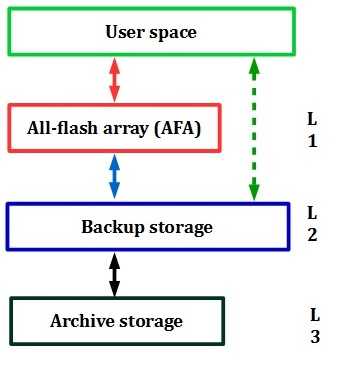
\includegraphics[width=7cm]{19_2018_Kliga1.jpg}
  %\caption{Конфигурация NFS v3}
  \label{Kliga1}
\end{figure}
\end{center} 
 

AFA-массивы на первом уровне (L1) при такой архитектурной реализации выступают в роли самостоятельных СХД, обеспечивающих высокую производительность для критически важных данных. По мере «остывания» данных они в режиме теневого копирования переносятся на второй уровень хранения на механических дисках с высокой скоростью вращения шпинделя. Удаление данных на первом уровне производится когда их показатель их востребовательности ниже установленного уровня определенного показателем «температуры данных», при этом при необходимости их резервная копия сохраняется на втором уровне хранения.

Данные со второго уровня хранения (L2) так же по мере «остывания» теневым копированием переносятся на третий архивный уровень (L3) на котором используются механические накопители большой емкости, но с низкой скоростью вращения шпинделя. Для хранения данных с некритичным временем доступа, в пользовательском пространстве создается точка монтирования на второй уровень (L2) СХД. Управление размещением данных на уровнях и организацией доступа к ним осуществляется с помощью контроллера SDS (software-defined storage), например, на базе решения openSDS~\cite{Klyga-8}.

Основные преимущества данного варианта создания гибридной СХД:

\begin{itemize}
  \item возможность обеспечения хранения данных с учетом требований к критичности времени доступа к данным;
  \item на каждом уровне отдельное хранилище данных может использоваться как самостоятельно устройства с функцией централизованного управления и возможностями резервного хранения данных;
  \item использование функционала теневого копирования для резервирования данных между отдельными хранилищами или уровнями;
  \item единый центр управления хранением данных на базе решений FOSS.
\end{itemize}

Основные недостатки:

\begin{itemize}
  \item невозможность использования технологии тиринга между уровнями хранения данных;
  \item высокая нагрузка на внутреннюю шину подключения хранилищ данных между уровнями из-за операций теневого копирования;
  \item сложность создания архитектуры и настройки под заданные параметры производительности.
\end{itemize}

Вторым вариантом реализации гибридного СХД с низким временем доступа  является использование возможностей накопителей с интерфейсом NVM Express, с двухуровневой схемой структурной схемой СХД с использованием технологии тиринга на первом уровне хранилища данных в массивах AFA (рисунок ниже). В основе этого варианта лежит концепция использования накопителей с интерфейсом  NVM Express в качестве элементов хранения данных RAM пользователя, и основным хранилищем данных на AFA-массивах.  Между двумя слоями в AFA первого уровня (L1) используется технология тиринга, когда «теплые данные из первого слоя переносятся во второй слой. Если же места для хранения данных исчерпано, либо данные стали <<остывшими>> они переносятся на второй уровень хранения (L2).

Этот вариант реализации гибридной СХД позволяет оптимально использовать возможности всех типов флеш-накопителей, а при необходимости возможности по хранению данных могут расширены за счет добавления новых уровней.

\begin{center}
\begin{figure}[h!]
  \centering
  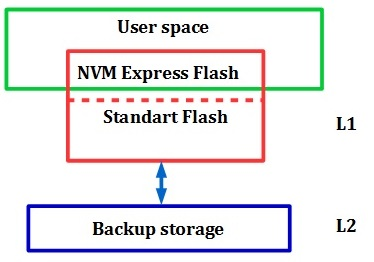
\includegraphics[width=7cm]{19_2018_Kliga2.jpg}
  %\caption{Конфигурация NFS v3}
  \label{Kliga2}
\end{figure}
\end{center} 

Основные преимущества данного варианта создания гибридной СХД:

\begin{itemize}
  \item возможность обеспечения высокой доступности данных;
  \item более простая схема реализации хранилища данных;
  \item использование функционала технологии тиринга и теневого копирования для резервирования данных между отдельными уровнями;
  \item высокая доступность данных для пользователя.
\end{itemize}

\begin{thebibliography}{20}
\bibitem{Klyga-1} Многослойные и многоуровненые системы хранения данных // LVEE 2017. \url{https://lvee.org/ru/abstracts/238}
\bibitem{Klyga-2} NVM Express: the official site. \url{http://www.nvmexpress.org/}
\bibitem{Klyga-3} Bcachefs: An advanced new filesystem for Linux. \url{https://bcachefs.org}
\bibitem{Klyga-4} ZFS: Zettabyte File System (OpenZFS project). \url{https://open-zfs.org}
\bibitem{Klyga-5} Btrfs: Btrfs is a modern CoW filesystem for Linux: // btrfs official site. \url{https://btrfs.wiki.kernel.org/index.php/Main\_Page}
\bibitem{Klyga-6} Ceph: The future of storage. \url{https://ceph.com/}
\bibitem{Klyga-7} Gluster: Storage for your Cloud. \url{https://gluster.org}
\bibitem{Klyga-8} OpenSDS Project. \url{https://www.opensds.io/}
\end{thebibliography}
\end{document}

\documentclass[10pt, a5paper]{article}
\usepackage{pdfpages}
\usepackage{parallel}
\usepackage[T2A]{fontenc}
\usepackage{ucs}
\usepackage[utf8x]{inputenc}
\usepackage[polish,english,russian]{babel}
\usepackage{hyperref}
\usepackage{rotating}
\usepackage[inner=2cm,top=1.8cm,outer=2cm,bottom=2.3cm,nohead]{geometry}
\usepackage{listings}
\usepackage{graphicx}
\usepackage{wrapfig}
\usepackage{longtable}
\usepackage{indentfirst}
\usepackage{array}
\newcolumntype{P}[1]{>{\raggedright\arraybackslash}p{#1}}
\frenchspacing
\usepackage{fixltx2e} %text sub- and superscripts
\usepackage{icomma} % коскі ў матэматычным рэжыме
\PreloadUnicodePage{4}

\newcommand{\longpage}{\enlargethispage{\baselineskip}}
\newcommand{\shortpage}{\enlargethispage{-\baselineskip}}

\def\switchlang#1{\expandafter\csname switchlang#1\endcsname}
\def\switchlangbe{
\let\saverefname=\refname%
\def\refname{Літаратура}%
\def\figurename{Іл.}%
}
\def\switchlangen{
\let\saverefname=\refname%
\def\refname{References}%
\def\figurename{Fig.}%
}
\def\switchlangru{
\let\saverefname=\refname%
\let\savefigurename=\figurename%
\def\refname{Литература}%
\def\figurename{Рис.}%
}

\hyphenation{admi-ni-stra-tive}
\hyphenation{ex-pe-ri-ence}
\hyphenation{fle-xi-bi-li-ty}
\hyphenation{Py-thon}
\hyphenation{ma-the-ma-ti-cal}
\hyphenation{re-ported}
\hyphenation{imp-le-menta-tions}
\hyphenation{pro-vides}
\hyphenation{en-gi-neering}
\hyphenation{com-pa-ti-bi-li-ty}
\hyphenation{im-pos-sible}
\hyphenation{desk-top}
\hyphenation{elec-tro-nic}
\hyphenation{com-pa-ny}
\hyphenation{de-ve-lop-ment}
\hyphenation{de-ve-loping}
\hyphenation{de-ve-lop}
\hyphenation{da-ta-ba-se}
\hyphenation{plat-forms}
\hyphenation{or-ga-ni-za-tion}
\hyphenation{pro-gramming}
\hyphenation{in-stru-ments}
\hyphenation{Li-nux}
\hyphenation{sour-ce}
\hyphenation{en-vi-ron-ment}
\hyphenation{Te-le-pathy}
\hyphenation{Li-nux-ov-ka}
\hyphenation{Open-BSD}
\hyphenation{Free-BSD}
\hyphenation{men-ti-on-ed}
\hyphenation{app-li-ca-tion}

\def\progref!#1!{\texttt{#1}}
\renewcommand{\arraystretch}{2} %Іначай формулы ў матрыцы зліпаюцца з лініямі
\usepackage{array}

\def\interview #1 (#2), #3, #4, #5\par{

\section[#1, #3, #4]{#1 -- #3, #4}
\def\qname{LVEE}
\def\aname{#1}
\def\q ##1\par{{\noindent \bf \qname: ##1 }\par}
\def\a{{\noindent \bf \aname: } \def\qname{L}\def\aname{#2}}
}

\def\interview* #1 (#2), #3, #4, #5\par{

\section*{#1\\{\small\rm #3, #4. #5}}

\def\qname{LVEE}
\def\aname{#1}
\def\q ##1\par{{\noindent \bf \qname: ##1 }\par}
\def\a{{\noindent \bf \aname: } \def\qname{L}\def\aname{#2}}
}

\begin{document}
\title{Постобработка фотографий в программе darktable\footnote{\url{vle@gmx.net}, \url{https://lvee.org/en/abstracts/292}}}
\author{Aleksey Cheusov, Minsk, Belarus}
\maketitle
\begin{abstract}
Darktable is an open source application devoted to processing of RAW
files. The program can manage collections of RAWs with rating, color
labels and custom tags. A rich set of built-in filters, used at
processing, store their settings in a form of a history stack, which
is saved alongside original RAW, providing original RAW
untouched.
\end{abstract}
Программа обработки графических изображений darktabkle уже поднималась
на LVEE в 2011-м году. Поэтому настоящий доклад не столько посвящен
описанию его возможностей, а модулей в системе несколько десятков,
сколько представляет собой набор примеров того, в каких ситуациях
какой модуль или какие модули можно использовать и каким
образом. Привести исчерпывающие примеры для всех модулей и ситуаций
вряд ли возможно, ввиду огромного их количества, но я попытаюсь кратко
описать наиболее типичные ситуации.

\subsection*{Маски}

Все программы для обработки фото имеют возможность наложить какой-либо
фильтр или эффект на часть фотографии. Например, обрабатываемая
область может быть нарисована вручную кистью или ограничена
многоугольником. Такая же возможность есть и в darktable. Но я хотел
бы особенно отметить наличие так называемых parametric masks. С их
помощью можно задать область фотографии, ограниченную данными в
каналах Lightness, a и b в цветовом пространстве Lab, а также Chroma и
hue в цветовом пространстве LCh. В совокупности с возможностью
выполнения логических операций над масками это дает очень мощные
возможности по точной <<прорисовке>> области применения того или иного
эффекта.

\subsection*{Коррекция экспозиции и контрастность изображения}

Иногда бывает так, что при сьемке неправильно выставлена
экспозиция. Таким образом снимок получается частично
переэкспонированным или недоэкспонированным. Это также происходит в
случаях, когда динамического диапазона камеры не хватает для того,
чтобы полностью передать все детали снимаемого объекта, например,
яркого солнечного неба и глубоких теней. Самым простым способом
исправить это является модуль exposition. Что касается контрастности,
то здесь можно использовать модули levels, tone curve, contrast
brightness saturation, zone systems и shadows and highlights. Лично я
практически никогда не использую модули contrast brightness saturation
и shadows and highlights для этих целей, поскольку модули levels, zone
systems и tone curve предоставляют гораздо больше возможностей для
этого. Недостаток контраста возникает почти всегда при сЪемке, например,
<<типичной белорусской зимой>>, когда картинка по большому счету
представляет собой <<серое на сером>>. В этом случае необходимо
выставить точки белого и черного в модуле levels. Честно говоря, этот
модуль я использую практически всегда. Именно с него начинается
обработка практически любого снимка. Настройка точки белого и черного
также помогает избавиться от лишних деталей в тенях и свете, и придает
фотографии большую драматичность или концентрирует внимание на
основном объекте съемки. Модули tone curve и zone systems очень похожи
по функциональности, но я предпочитаю zone systems для обработки
черно-белых фотографий.

\subsection*{Кадрирование, выравнивание горизонта и коррекция геометрии}

Практически все кадры после сьемки нуждаются в кадрировании. За это
отвечает модуль crop and rotate. Этот же модуль можно использоать для
исправления <<заваленного>> горизонта. При съемке высотных зданий,
особенно с близкого расстояния, возникают геометрические искажения,
что так же можно исправить этим модулем или модулем perspective
correction.

\subsection*{Цветокоррекция, насыщенность}

Для придания фотографии нужной атмосферы можно не только
корректировать освещенность (lightness в цветовой схеме Lab), но и
влиять на цвета. Это можно сделать с помощью модулей white balance,
velvia, vibrance, color zones, contrast brightness saturation а также
color contrast, color mapping, color reconstruction и colorize. Так же
как и в fotoshop (PS), darktable позволяет изменять цвета по всему
цветовому кругу, что дает возможность создать монохромную фотографию
или оставить только хорошо сочетающиеся друг с другом цвета.

\subsection*{Шумоподавление, ХА, увеличение резкости, микроконтраст и т.п.}

Любая камера, особенно при повышенных ISO, добавляет шумы в кадр. Их
количество можно уменьшить с использованием модулей raw denoise,
denoise (profiled), denoise (bilateral filter) и denoise (non-local
means).  Хроматические аберрации можно убрать с помощью модулей
chromatic aberrations и defringe.  Скорректировать дисторсию, вносимую
объективом, можно исправить модулем lens correction. В этом случае
используется постоянно пополняемая база данных
объективов. Виньетирование, вносимое объективами на открытых
диафрагмах, можно исправить с помощью модуля vignetting. С его же
помощью можно его добавить, например, для портретов.

\subsection*{Обработка лица и кожи}

Часто возникает необходимость ретушировать кожу человека на снимках и
убрать недостатки, видимые на фотографии, особенно на снимках с
лицевым портретом. Для этого можно воспользоваться модулями spot
removal и equalizer. Equalizer может так же использоваться для
увеличения микро- и макро-контраста на уровнях света и цвета. Для
улучшения резкости изображения можно поспользоваться модулем sharpen.

\subsection*{Черно-белая фотография}

Кажется, черно-белая фотография никогда не потеряет своей
актуальности. В darktable есть много способов реализовать это, но я
предпочитаю два модуля: monochrome и color zones. Последний дает
возможность преобразовать различные цвета в разные оттенки серого.

\subsection*{Другие возможности}

Есть ряд других модулей, с помощью которых можно добавить подпись к
фотографии (watermark), добавить зернистости по аналогии с пленочной
фотографией (grain), поместить фотографию в рамочку (framing) и многое
другое.

\subsection*{Выводы}

На мой взгляд, darktable представляет собой профессиональный
инструмент для постобработки фотографий, по совокупности факторов не
уступающий по свои возможностям, таким известным программам как
photoshop, lightroom и capture one. Лично мне не хватает разьве что
поканальных RGB кривых для получения <<чистого>> черного цвета и более
богатых средств ретуширования.

\end{document}

\documentclass[10pt, a5paper]{article}
\usepackage{pdfpages}
\usepackage{parallel}
\usepackage[T2A]{fontenc}
\usepackage{ucs}
\usepackage[utf8x]{inputenc}
\usepackage[polish,english,russian]{babel}
\usepackage{hyperref}
\usepackage{rotating}
\usepackage[inner=2cm,top=1.8cm,outer=2cm,bottom=2.3cm,nohead]{geometry}
\usepackage{listings}
\usepackage{graphicx}
\usepackage{wrapfig}
\usepackage{longtable}
\usepackage{indentfirst}
\usepackage{array}
\newcolumntype{P}[1]{>{\raggedright\arraybackslash}p{#1}}
\frenchspacing
\usepackage{fixltx2e} %text sub- and superscripts
\usepackage{icomma} % коскі ў матэматычным рэжыме
\PreloadUnicodePage{4}

\newcommand{\longpage}{\enlargethispage{\baselineskip}}
\newcommand{\shortpage}{\enlargethispage{-\baselineskip}}

\def\switchlang#1{\expandafter\csname switchlang#1\endcsname}
\def\switchlangbe{
\let\saverefname=\refname%
\def\refname{Літаратура}%
\def\figurename{Іл.}%
}
\def\switchlangen{
\let\saverefname=\refname%
\def\refname{References}%
\def\figurename{Fig.}%
}
\def\switchlangru{
\let\saverefname=\refname%
\let\savefigurename=\figurename%
\def\refname{Литература}%
\def\figurename{Рис.}%
}

\hyphenation{admi-ni-stra-tive}
\hyphenation{ex-pe-ri-ence}
\hyphenation{fle-xi-bi-li-ty}
\hyphenation{Py-thon}
\hyphenation{ma-the-ma-ti-cal}
\hyphenation{re-ported}
\hyphenation{imp-le-menta-tions}
\hyphenation{pro-vides}
\hyphenation{en-gi-neering}
\hyphenation{com-pa-ti-bi-li-ty}
\hyphenation{im-pos-sible}
\hyphenation{desk-top}
\hyphenation{elec-tro-nic}
\hyphenation{com-pa-ny}
\hyphenation{de-ve-lop-ment}
\hyphenation{de-ve-loping}
\hyphenation{de-ve-lop}
\hyphenation{da-ta-ba-se}
\hyphenation{plat-forms}
\hyphenation{or-ga-ni-za-tion}
\hyphenation{pro-gramming}
\hyphenation{in-stru-ments}
\hyphenation{Li-nux}
\hyphenation{sour-ce}
\hyphenation{en-vi-ron-ment}
\hyphenation{Te-le-pathy}
\hyphenation{Li-nux-ov-ka}
\hyphenation{Open-BSD}
\hyphenation{Free-BSD}
\hyphenation{men-ti-on-ed}
\hyphenation{app-li-ca-tion}

\def\progref!#1!{\texttt{#1}}
\renewcommand{\arraystretch}{2} %Іначай формулы ў матрыцы зліпаюцца з лініямі
\usepackage{array}

\def\interview #1 (#2), #3, #4, #5\par{

\section[#1, #3, #4]{#1 -- #3, #4}
\def\qname{LVEE}
\def\aname{#1}
\def\q ##1\par{{\noindent \bf \qname: ##1 }\par}
\def\a{{\noindent \bf \aname: } \def\qname{L}\def\aname{#2}}
}

\def\interview* #1 (#2), #3, #4, #5\par{

\section*{#1\\{\small\rm #3, #4. #5}}

\def\qname{LVEE}
\def\aname{#1}
\def\q ##1\par{{\noindent \bf \qname: ##1 }\par}
\def\a{{\noindent \bf \aname: } \def\qname{L}\def\aname{#2}}
}

\begin{document}
\title{Запуск Jenkins на спот-инстансах AWS\footnote{\url{delgod@delgod.com}, \url{https://lvee.org/en/abstracts/293}}}
\author{Mykola Marzhan, Kyiv, Ukraine}
\maketitle
\begin{abstract}
A case of Jenkins CI/CD system in AWS cloud is reviewed, featuring use of spot instances, which are extemely cheap but are affected with arbitrary shutdowns in any time by the cloud provider. An approach to run Jenkins master on spot instances in AWS with fault tolerance and automatic fault recovery is proposed. Comparison of plugins which allow to run worker nodes on spot instances on-demand is presented.
\end{abstract}
\subsection*{Введение и постановка задачи}

Jenkins~--- это популярная система непрерывной интеграции и непрерывной доставки (CI/CD), которая на текущий момент представляет собой наиболее расширяемое CI/CD-решение на рынке, с огромным количеством плагинов для интеграции со всем на свете. В числе прочего для Jenkins можно найти достаточное число вариантов запуска задач в облаке по запросу (когда виртуальная машина каждый раз  запускается под конкретную задачу, а затем уничтожается).

В системе Jenkins испольузются узлы двух типов: master и\linebreak worker. В базовой конфигурации задачи могут выполняются на master-узле. В более сложном варианте master делегирует выполнение задач worker-узлам, автоматически выбирая наиболее подходящий из них. В отличие от master-узла, на worker-ах запущен не полноценный Jenkins, а т.н. worker agent~--- программная прослойка, минимально необходимая для запуска задач по запросу.

Применительно к облачным технологиям (и, в частности, AWS) такая архитектура очевидно легко переносится на инстансы по требованию (on-demand instances). Однако в настоящей работе предлагается вариант конфигурации Jenkins, использующий спот-\linebreak инстансы Amazon EC2.

Spot instances~--- это такие же вычислительные ресурсы, выделяемые в облаке AWS, как и более традиционные инстансы по требованию. Однако в отличие от последних спот-инстансы доступны с большой скидкой. Ценой этой экономии средств является то, что работа спотов может быть в любой момент прервана со стороны AWS (с  уведомлением за две минуты) в случае, если AWS требуются ресурсы.

\subsection*{Сохранение данных master-узла}

Первой задачей, необходимой для обеспечения работы master-узла Jenkins в таких условиях, является сохранение данных при уничтожении инстанса и их подгрузка при его перезапуске. Можно выделить два варианта для такого сохраняемого хранилища:

\begin{itemize}
  \item EFS (Elastic File System)~--- NFS, который запускается на AWS в 1 клик. Его недостатком является низкое быстродействие, а преимуществом~--- автоматическое копирование данных между availability zones (независимыми датацентрами в одной локации), это значит что master-узел может быть перезапущен в любой из них.
  \item EBS (Elastic Block Storage)~--- диск, который видится внутри инстанса как блочное устройство. Преимущество этого варианта~--- высокое быстродействие, а недостаток~--- возможность запуска master-узела только в пределах одного датацентра (availability zone).
\end{itemize}

В случае EFS при загрузке спота монтируется NFS-директория, и Jenkins получает доступ к базе. В случае EBS, инстанс после загрузки присоединяет к себе нужное независимое блочное устройство через AWS cli.

\subsection*{Запуск и остановка master-узла}

Как уже было упомянуто, на старте инстанс с master-узлом монтирует EFS или EBS со всей файловой базой. Затем запускается Java-процесс, в результате чего Jenkins воспринимает ситуацию не как перемещение на другой узел, а как простой перезапуск.

При внеплановой остановке master-узла сохранить состояние помогает двухминутное оповещение. По его получении выполняется остановка Jenkins и размонтируется файловое хранилище. Чтобы была гарантия, что файловая база не окажется в промежуточном (повреждённом) состоянии, используется MAX\_SURVIVABILITY режим в Jenkins. Кроме того, задачи не запускаются на master-узле, а только на worker-узлах. Использование исключительно MAX\_SURVIVABILITY и pipeline jobs, а также статического IP (Elastic IP) для master позволяет восстанавливать соединение с worker-\linebreak узлами, и таким образом перезагрузка master-узла в большинстве случаев не сказывается на задачах, выполняющихся в данный момент на worker'ах (разумеется, при рестарте worker-узлов выполнение на них задач завершается неудачей и требует повторного запуска вручную или автоматически при задании опции retry на уровне stage в declarative pipeline).

\subsection*{Запуск worker-узлов}

Взаимодействие с Amazon EC2 для запуска инстансов под выполнение задач может осуществляться с помощью двух плагинов Jenkins:

\begin{itemize}
  \item EC2 Fleet Jenkins Plugin~--- плагин, написанный для Jenkins сотрудниками Amazon. С его помощью master-узел Jenkins информирует AWS, сколько инстансов для worker-узлов необходимо запустить. Его особенностью является то, что вся конфигурация хранится на стороне AWS, а также работоспособность вне пределов одной availability zone.
  \item Amazon EC2 plugin~--- аналогичный плагин, созданный комьюнити. Он является более популярным, однако worker-узлы с одним лейблом можно запускать только в пределах одной availability zone. В качестве его достоинства можно отметить хранение конфигурации непосредственно в Jenkins.
\end{itemize}

\subsection*{Вместо заключения}

Конфигурация, описывающая представленное решение, доступна публично по адресу \url{https://github.com/Percona-Lab/jenkins-} \url{pipelines/tree/master/IaC/ps.cd}.

\end{document}

%\documentclass[10pt, a5paper]{article}
\usepackage{pdfpages}
\usepackage{parallel}
\usepackage[T2A]{fontenc}
\usepackage{ucs}
\usepackage[utf8x]{inputenc}
\usepackage[polish,english,russian]{babel}
\usepackage{hyperref}
\usepackage{rotating}
\usepackage[inner=2cm,top=1.8cm,outer=2cm,bottom=2.3cm,nohead]{geometry}
\usepackage{listings}
\usepackage{graphicx}
\usepackage{wrapfig}
\usepackage{longtable}
\usepackage{indentfirst}
\usepackage{array}
\newcolumntype{P}[1]{>{\raggedright\arraybackslash}p{#1}}
\frenchspacing
\usepackage{fixltx2e} %text sub- and superscripts
\usepackage{icomma} % коскі ў матэматычным рэжыме
\PreloadUnicodePage{4}

\newcommand{\longpage}{\enlargethispage{\baselineskip}}
\newcommand{\shortpage}{\enlargethispage{-\baselineskip}}

\def\switchlang#1{\expandafter\csname switchlang#1\endcsname}
\def\switchlangbe{
\let\saverefname=\refname%
\def\refname{Літаратура}%
\def\figurename{Іл.}%
}
\def\switchlangen{
\let\saverefname=\refname%
\def\refname{References}%
\def\figurename{Fig.}%
}
\def\switchlangru{
\let\saverefname=\refname%
\let\savefigurename=\figurename%
\def\refname{Литература}%
\def\figurename{Рис.}%
}

\hyphenation{admi-ni-stra-tive}
\hyphenation{ex-pe-ri-ence}
\hyphenation{fle-xi-bi-li-ty}
\hyphenation{Py-thon}
\hyphenation{ma-the-ma-ti-cal}
\hyphenation{re-ported}
\hyphenation{imp-le-menta-tions}
\hyphenation{pro-vides}
\hyphenation{en-gi-neering}
\hyphenation{com-pa-ti-bi-li-ty}
\hyphenation{im-pos-sible}
\hyphenation{desk-top}
\hyphenation{elec-tro-nic}
\hyphenation{com-pa-ny}
\hyphenation{de-ve-lop-ment}
\hyphenation{de-ve-loping}
\hyphenation{de-ve-lop}
\hyphenation{da-ta-ba-se}
\hyphenation{plat-forms}
\hyphenation{or-ga-ni-za-tion}
\hyphenation{pro-gramming}
\hyphenation{in-stru-ments}
\hyphenation{Li-nux}
\hyphenation{sour-ce}
\hyphenation{en-vi-ron-ment}
\hyphenation{Te-le-pathy}
\hyphenation{Li-nux-ov-ka}
\hyphenation{Open-BSD}
\hyphenation{Free-BSD}
\hyphenation{men-ti-on-ed}
\hyphenation{app-li-ca-tion}

\def\progref!#1!{\texttt{#1}}
\renewcommand{\arraystretch}{2} %Іначай формулы ў матрыцы зліпаюцца з лініямі
\usepackage{array}

\def\interview #1 (#2), #3, #4, #5\par{

\section[#1, #3, #4]{#1 -- #3, #4}
\def\qname{LVEE}
\def\aname{#1}
\def\q ##1\par{{\noindent \bf \qname: ##1 }\par}
\def\a{{\noindent \bf \aname: } \def\qname{L}\def\aname{#2}}
}

\def\interview* #1 (#2), #3, #4, #5\par{

\section*{#1\\{\small\rm #3, #4. #5}}

\def\qname{LVEE}
\def\aname{#1}
\def\q ##1\par{{\noindent \bf \qname: ##1 }\par}
\def\a{{\noindent \bf \aname: } \def\qname{L}\def\aname{#2}}
}

%\frenchspacing
\begin{document}
\title{Голос спонсора: ITS Partner}
%\author{}
\date{}
\maketitle%

~

\end{document}



%\documentclass[10pt, a5paper]{article}
\usepackage{pdfpages}
\usepackage{parallel}
\usepackage[T2A]{fontenc}
\usepackage{ucs}
\usepackage[utf8x]{inputenc}
\usepackage[polish,english,russian]{babel}
\usepackage{hyperref}
\usepackage{rotating}
\usepackage[inner=2cm,top=1.8cm,outer=2cm,bottom=2.3cm,nohead]{geometry}
\usepackage{listings}
\usepackage{graphicx}
\usepackage{wrapfig}
\usepackage{longtable}
\usepackage{indentfirst}
\usepackage{array}
\newcolumntype{P}[1]{>{\raggedright\arraybackslash}p{#1}}
\frenchspacing
\usepackage{fixltx2e} %text sub- and superscripts
\usepackage{icomma} % коскі ў матэматычным рэжыме
\PreloadUnicodePage{4}

\newcommand{\longpage}{\enlargethispage{\baselineskip}}
\newcommand{\shortpage}{\enlargethispage{-\baselineskip}}

\def\switchlang#1{\expandafter\csname switchlang#1\endcsname}
\def\switchlangbe{
\let\saverefname=\refname%
\def\refname{Літаратура}%
\def\figurename{Іл.}%
}
\def\switchlangen{
\let\saverefname=\refname%
\def\refname{References}%
\def\figurename{Fig.}%
}
\def\switchlangru{
\let\saverefname=\refname%
\let\savefigurename=\figurename%
\def\refname{Литература}%
\def\figurename{Рис.}%
}

\hyphenation{admi-ni-stra-tive}
\hyphenation{ex-pe-ri-ence}
\hyphenation{fle-xi-bi-li-ty}
\hyphenation{Py-thon}
\hyphenation{ma-the-ma-ti-cal}
\hyphenation{re-ported}
\hyphenation{imp-le-menta-tions}
\hyphenation{pro-vides}
\hyphenation{en-gi-neering}
\hyphenation{com-pa-ti-bi-li-ty}
\hyphenation{im-pos-sible}
\hyphenation{desk-top}
\hyphenation{elec-tro-nic}
\hyphenation{com-pa-ny}
\hyphenation{de-ve-lop-ment}
\hyphenation{de-ve-loping}
\hyphenation{de-ve-lop}
\hyphenation{da-ta-ba-se}
\hyphenation{plat-forms}
\hyphenation{or-ga-ni-za-tion}
\hyphenation{pro-gramming}
\hyphenation{in-stru-ments}
\hyphenation{Li-nux}
\hyphenation{sour-ce}
\hyphenation{en-vi-ron-ment}
\hyphenation{Te-le-pathy}
\hyphenation{Li-nux-ov-ka}
\hyphenation{Open-BSD}
\hyphenation{Free-BSD}
\hyphenation{men-ti-on-ed}
\hyphenation{app-li-ca-tion}

\def\progref!#1!{\texttt{#1}}
\renewcommand{\arraystretch}{2} %Іначай формулы ў матрыцы зліпаюцца з лініямі
\usepackage{array}

\def\interview #1 (#2), #3, #4, #5\par{

\section[#1, #3, #4]{#1 -- #3, #4}
\def\qname{LVEE}
\def\aname{#1}
\def\q ##1\par{{\noindent \bf \qname: ##1 }\par}
\def\a{{\noindent \bf \aname: } \def\qname{L}\def\aname{#2}}
}

\def\interview* #1 (#2), #3, #4, #5\par{

\section*{#1\\{\small\rm #3, #4. #5}}

\def\qname{LVEE}
\def\aname{#1}
\def\q ##1\par{{\noindent \bf \qname: ##1 }\par}
\def\a{{\noindent \bf \aname: } \def\qname{L}\def\aname{#2}}
}

\begin{document}
\title{Голос спонсора: EPAM Systems}
%\author{}
\date{}
\maketitle

Компания EPAM Systems не первый год является спонсором международной конференции разработчиков и пользователей свободного программного обеспечения LVEE (Linux Vacation / Eastern Europe). Этот год также не стал исключением. Пожалуй, LVEE является самым значимым событием для русскоязычных разработчиков и тестировщиков Open Source. Каждое лето здесь встречаются начинающие специалисты и «ветераны»"=разработчики из десятка стран для обмена опытом и общения на профессиональные темы. Наши специалисты также активно участвуют в данной конференции: в качестве докладчиков и организаторов/волонтёров. Это уникальная в своём роде конференция, и именно поэтому EPAM Systems очередной раз принимает участие в LVEE в качестве спонсора.


EPAM Systems "--- одна из крупнейших компаний"=поставщиков\linebreak услуг в области разработки программного обеспечения и решений на территории СНГ и Центральной и Восточной Европы. Созданная в 1993 году, сегодня она имеет представительства в 12 странах мира, в штате работают более 9 тыс. сотрудников, из которых более 3 тыс. "--- в Беларуси. Рост компании обеспечивается за счет собственных обучающих программ и передаче опыта от больших специалистов до начинающих разработчиков. Компания EPAM Systems выполняет проекты более чем в 30 странах мира. Основные направления деятельности: разработка, тестирование, сопровождение и поддержка заказного программного обеспечения и бизнес"=приложений, а также ИТ"=консалтинг с учетом отраслевой специфики бизнеса.

Наша компания участвует в проектах с такими крупными, хорошо известными заказчиками как Google, Novell, Infoblox, Parallels, 10Gen и др., так и с небольшими, в том числе и с начинающими свой путь в софтверном бизнесе.


К примеру, для Infoblox была реализована связка между WebUI с BIND и DHCP. Для этого был разработан комплекс решений под управлением Shell и Python скриптов, а также механизм позволяющий вносить правки в BIND и DHCP на языке C. Также был разработан развернутый функционал, автоматизирующий инсталляцию новых устройств и их эксплуатацию, что позволяет значительно упростить управление данными. Встроенный Web"=интерфейс позволяет разворачивать, управлять сервисами DNS, DNSSEC, DHCP, IPAM, устанавливать новые версии ПО, архивировать и восстанавливать из архивов необходимые данные, восстанавливать их после аварии, проводить мониторинг сети и создавать отчеты без необходимости обращения к командной строке.


Еще одним решением, реализованным для компании Infoblox, являлся программный продукт, позволяющий контролировать сетевые изменения, таким образом, облегчая идентификацию трудноуловимых проблем конфигурации и соответствие требованиям. Вместо того чтобы просто регистрировать изменения, система использует внесенную информацию для проверки, анализа и автоматической обработки сетевых изменений. Благодаря инновационной, квалифицированной, глубокой технике логического анализа, программа изолирует проблемы исправности и конфигурации до того, как они могут вызвать более серьезные сбои.


Разработанная для анализа сложных сетей система изучает сеть, собирает ключевую информацию, применяет встроенную технику логического анализа и создает оценку исправности сети и список проблем, требующих принятие мер для улучшения качества работы сети.


Правильное использование свободного ПО в разработках сокращает и расходы на покупку лицензионных программ, и трудозатраты при создании коммерческого ПО. Немалую роль для достижения превосходного результата играет привлечение к разработке опытных специалистов. LVEE способствует появлению таких специалистов, развитию их навыков и расширению кругозора. Хотелось бы пожелать участникам конференции интересных проектов и максимум пользы от участия в LVEE.


\end{document}



%\documentclass[10pt, a5paper]{article}
\usepackage{pdfpages}
\usepackage{parallel}
\usepackage[T2A]{fontenc}
\usepackage{ucs}
\usepackage[utf8x]{inputenc}
\usepackage[polish,english,russian]{babel}
\usepackage{hyperref}
\usepackage{rotating}
\usepackage[inner=2cm,top=1.8cm,outer=2cm,bottom=2.3cm,nohead]{geometry}
\usepackage{listings}
\usepackage{graphicx}
\usepackage{wrapfig}
\usepackage{longtable}
\usepackage{indentfirst}
\usepackage{array}
\newcolumntype{P}[1]{>{\raggedright\arraybackslash}p{#1}}
\frenchspacing
\usepackage{fixltx2e} %text sub- and superscripts
\usepackage{icomma} % коскі ў матэматычным рэжыме
\PreloadUnicodePage{4}

\newcommand{\longpage}{\enlargethispage{\baselineskip}}
\newcommand{\shortpage}{\enlargethispage{-\baselineskip}}

\def\switchlang#1{\expandafter\csname switchlang#1\endcsname}
\def\switchlangbe{
\let\saverefname=\refname%
\def\refname{Літаратура}%
\def\figurename{Іл.}%
}
\def\switchlangen{
\let\saverefname=\refname%
\def\refname{References}%
\def\figurename{Fig.}%
}
\def\switchlangru{
\let\saverefname=\refname%
\let\savefigurename=\figurename%
\def\refname{Литература}%
\def\figurename{Рис.}%
}

\hyphenation{admi-ni-stra-tive}
\hyphenation{ex-pe-ri-ence}
\hyphenation{fle-xi-bi-li-ty}
\hyphenation{Py-thon}
\hyphenation{ma-the-ma-ti-cal}
\hyphenation{re-ported}
\hyphenation{imp-le-menta-tions}
\hyphenation{pro-vides}
\hyphenation{en-gi-neering}
\hyphenation{com-pa-ti-bi-li-ty}
\hyphenation{im-pos-sible}
\hyphenation{desk-top}
\hyphenation{elec-tro-nic}
\hyphenation{com-pa-ny}
\hyphenation{de-ve-lop-ment}
\hyphenation{de-ve-loping}
\hyphenation{de-ve-lop}
\hyphenation{da-ta-ba-se}
\hyphenation{plat-forms}
\hyphenation{or-ga-ni-za-tion}
\hyphenation{pro-gramming}
\hyphenation{in-stru-ments}
\hyphenation{Li-nux}
\hyphenation{sour-ce}
\hyphenation{en-vi-ron-ment}
\hyphenation{Te-le-pathy}
\hyphenation{Li-nux-ov-ka}
\hyphenation{Open-BSD}
\hyphenation{Free-BSD}
\hyphenation{men-ti-on-ed}
\hyphenation{app-li-ca-tion}

\def\progref!#1!{\texttt{#1}}
\renewcommand{\arraystretch}{2} %Іначай формулы ў матрыцы зліпаюцца з лініямі
\usepackage{array}

\def\interview #1 (#2), #3, #4, #5\par{

\section[#1, #3, #4]{#1 -- #3, #4}
\def\qname{LVEE}
\def\aname{#1}
\def\q ##1\par{{\noindent \bf \qname: ##1 }\par}
\def\a{{\noindent \bf \aname: } \def\qname{L}\def\aname{#2}}
}

\def\interview* #1 (#2), #3, #4, #5\par{

\section*{#1\\{\small\rm #3, #4. #5}}

\def\qname{LVEE}
\def\aname{#1}
\def\q ##1\par{{\noindent \bf \qname: ##1 }\par}
\def\a{{\noindent \bf \aname: } \def\qname{L}\def\aname{#2}}
}

\begin{document}
\title{Голос спонсора: SaM Solutions}
%\author{}
\date{}
\maketitle

Компания SaM Solutions выступает в роли системо-образующего спонсора конференции Linux Vacation Eastern Europe с момента рождения LVEE в 2005 году и на протяжении всех лет её проведения. 

Сложившаяся корпоративная практика не случайна. Продукты и решения, задействующие Linux и другие Free/Open Source Software проекты, составляют заметную часть пакета разработок SaM Solutions. Кадровая политика компании направлена на поощрение профессионального развития своих сотрудников, организацию их эффективного отдыха и привлечение хорошо мотивированных кандидатов к работе на компанию. Формат конференции LVEE успешно позволяет решать все три задачи. 

Одним из подразделений компании является отдел Linux и \linebreak Embbeded. Специалисты компании на протяжении десятилетий работают с СПО. Компанией реализован ряд проектов по адаптации ОС GNU/Linux для работы в различных устройствах, построенных на таких платформах как ARM, PowerPC, x86, MIPS. В последние годы "--- на ведущие позиции выходит разработка управляющего ПО для серверов Enterprise-класса, от низкоуровнего BMC Firmware на основе Linux до высокоуровневых систем контроля виртуализации и графических интерфейсов управления, от прошивок устройств хранения данных до BSP интегрированных плат для разработчика. Надёжность, качество и широкая функциональность множества свободных проектов позволяет строить нам системы любого уровня и сложности, опираясь на высококачественные готовые компоненты.

В рамках направления Linux и Embedded успешно выполнены проекты для таких знаковых заказчиков, как  Novell/SUSE, Fujitsu Technology Solutions  и осуществляется партнёрство с компаниями IBM и Oracle/Sun в области Open Source решений.

Мы разрабатываем, модифицируем и адаптируем различное свободное программное обеспечение для наших заказчиков, но не забываем и о своих нуждах "--- наши сотрудники используют в своей работе существующие програмные продукты и вносят вклад в их развитие. Часть внутренней инфраструктуры, а именно интранет-сеть компании, тестовые стенды отдела контроля качества, рабочие места сотрудников профильных подразделений "--- также работает под управлением СПО (серверные и десктопные платформы GNU/Linux и FreeBSD). 

В минувшем году, в рамках реорганизации, был разработан долгосрочный план развития направления Linux и Embedded в SaM Solutions. В нём впервые были кодифицированы уже имеющиеся внутренние неофициальные практики по взаимодействию с commu"=nity-based проектами. В частности разработаны меры и правила по
\begin{itemize}
  \item возврата изменений в родительские проекты (upstreaming);
  \item вхождения в состав постоянных разработчиков активно используемых нами FOSS-компонентов;
  \item публикации сообщений об ошибках (bug reporting);
  \item участия и помощи в организации community events;
  \item стимуляции докладов и участия в технических конференциях.
\end{itemize}
И план немедленно начал претворяться в жизнь.

Силами отдела организовано внутреннее обучение сотрудников на регулярной
основе. Был прочтен и опубликован курс по TDD. По согласованию с автором
опубликован курс Debian/Ubuntu Packaging (видео, презентация и исходные
тексты презентации в \LaTeX).  Были организованы и проведены курсы по
обучению QA специалистов для направления Embeded Linux. Проведено
практическое занятие по основам виртуализации и эмуляции, организована
лекция по вопросу профилирования и оптимизации Ruby-кода, лекция о
High-availability кластерах и направлении развития технологии. Кроме того,
проводился семинар по Video4Linux2. Для создания и обучения кадрового
резерва на ближайшее будущее запланированы постоянно действующие внутренние
проекты в области Embedded Linux, результаты которых также запланированы к
публикации.

Визиты представительных делегаций на Embedded World 2012 и Linux Con Europe/Embedded LinuxCon Europe 2011 обогатили нас новыми идеями, куда можно
двигаться дальше и что сейчас актуально. А выступления на Software
Engineering Forum for Students, круглом столе по СПО в рамках TIBO-2012
и LVEE Winter 2012 позволили поделиться опытом с
заинтересованными сторонами.

В апреле состоялась Ганноверская промышленная ярмарка \linebreak (Hannover Messe
2013). Компания SaM Solutions была представлена отдельным стендом, на
котором демонстрировались наработки в области встроенного и системного ПО
на базе OS Linux. Идея «умного» дома вызвала неподдельный интерес у
посетителей стенда.

При поддержке SaM Solutions, с декабря 2011 года возобновились регулярные встречи Minsk Linux Users Groups, под названием <<Линуксовка в SaM Solutions>>. Техническое оснащение линуксовок и открытый формат встреч позволил им практически мгновенно стать заметным дискуссионным клубом по широкому спектру вопросов, прямо или косвенно связанных с СПО. Свободная картография (OpenStreetMap), технологии виртуализации, минский \linebreak hackerspace, Linux Mobile, бойкот Голливудской продукции, systemd, загрузчик u-boot, белорусская локализация GNOME --- это только часть тем, поднятых за последние линуксовки.

Быстрые и положительные изменения, как внутри компании SaM Solutions, так и в экосфере СПО (и Linux в частности) наполняют нас уверенностью, что направление движения выбрано верно.

\begin{figure}[h!]
\centering
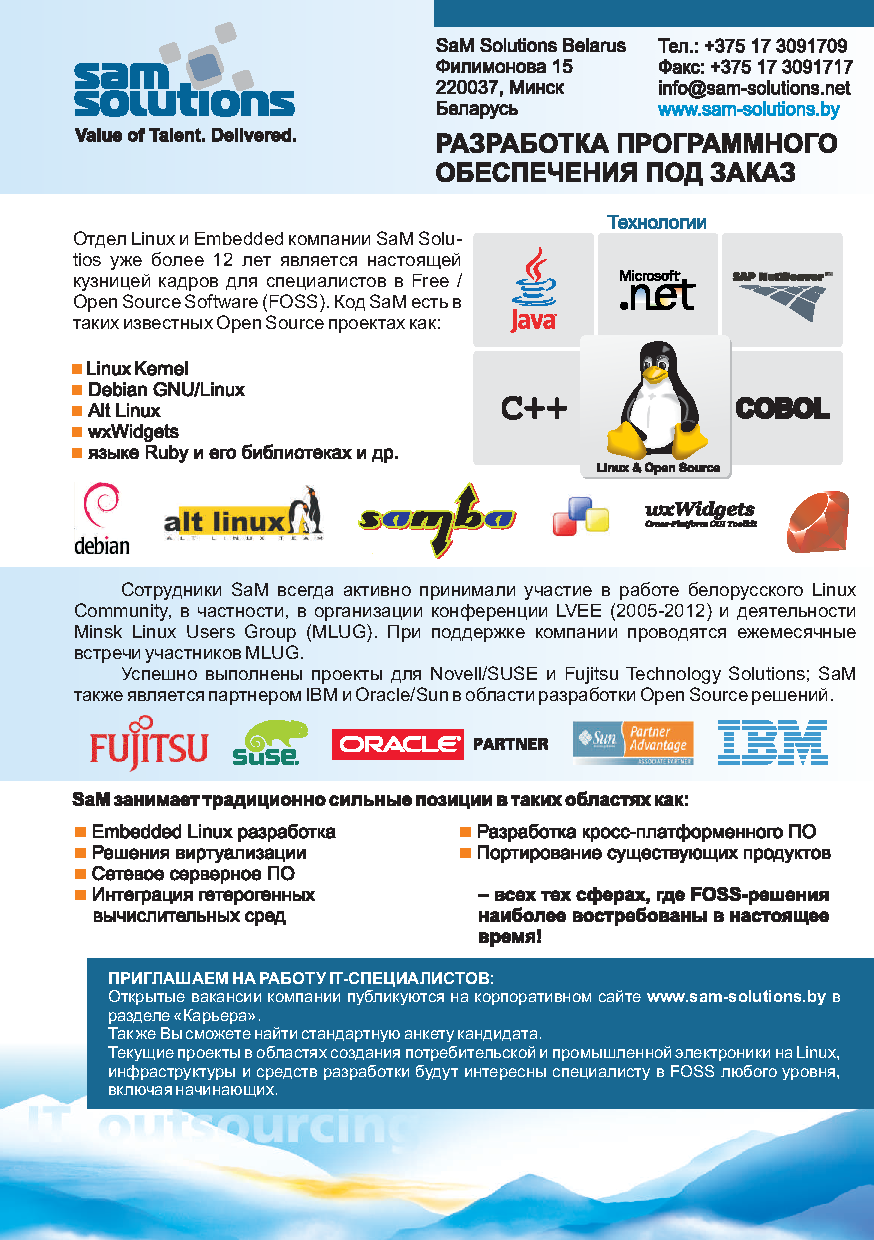
\includegraphics[height=11.8cm]{48_spons_sams.pdf}
\end{figure}
\end{document}



%\documentclass[10pt, a5paper]{article}
\usepackage{pdfpages}
\usepackage{parallel}
\usepackage[T2A]{fontenc}
\usepackage{ucs}
\usepackage[utf8x]{inputenc}
\usepackage[polish,english,russian]{babel}
\usepackage{hyperref}
\usepackage{rotating}
\usepackage[inner=2cm,top=1.8cm,outer=2cm,bottom=2.3cm,nohead]{geometry}
\usepackage{listings}
\usepackage{graphicx}
\usepackage{wrapfig}
\usepackage{longtable}
\usepackage{indentfirst}
\usepackage{array}
\newcolumntype{P}[1]{>{\raggedright\arraybackslash}p{#1}}
\frenchspacing
\usepackage{fixltx2e} %text sub- and superscripts
\usepackage{icomma} % коскі ў матэматычным рэжыме
\PreloadUnicodePage{4}

\newcommand{\longpage}{\enlargethispage{\baselineskip}}
\newcommand{\shortpage}{\enlargethispage{-\baselineskip}}

\def\switchlang#1{\expandafter\csname switchlang#1\endcsname}
\def\switchlangbe{
\let\saverefname=\refname%
\def\refname{Літаратура}%
\def\figurename{Іл.}%
}
\def\switchlangen{
\let\saverefname=\refname%
\def\refname{References}%
\def\figurename{Fig.}%
}
\def\switchlangru{
\let\saverefname=\refname%
\let\savefigurename=\figurename%
\def\refname{Литература}%
\def\figurename{Рис.}%
}

\hyphenation{admi-ni-stra-tive}
\hyphenation{ex-pe-ri-ence}
\hyphenation{fle-xi-bi-li-ty}
\hyphenation{Py-thon}
\hyphenation{ma-the-ma-ti-cal}
\hyphenation{re-ported}
\hyphenation{imp-le-menta-tions}
\hyphenation{pro-vides}
\hyphenation{en-gi-neering}
\hyphenation{com-pa-ti-bi-li-ty}
\hyphenation{im-pos-sible}
\hyphenation{desk-top}
\hyphenation{elec-tro-nic}
\hyphenation{com-pa-ny}
\hyphenation{de-ve-lop-ment}
\hyphenation{de-ve-loping}
\hyphenation{de-ve-lop}
\hyphenation{da-ta-ba-se}
\hyphenation{plat-forms}
\hyphenation{or-ga-ni-za-tion}
\hyphenation{pro-gramming}
\hyphenation{in-stru-ments}
\hyphenation{Li-nux}
\hyphenation{sour-ce}
\hyphenation{en-vi-ron-ment}
\hyphenation{Te-le-pathy}
\hyphenation{Li-nux-ov-ka}
\hyphenation{Open-BSD}
\hyphenation{Free-BSD}
\hyphenation{men-ti-on-ed}
\hyphenation{app-li-ca-tion}

\def\progref!#1!{\texttt{#1}}
\renewcommand{\arraystretch}{2} %Іначай формулы ў матрыцы зліпаюцца з лініямі
\usepackage{array}

\def\interview #1 (#2), #3, #4, #5\par{

\section[#1, #3, #4]{#1 -- #3, #4}
\def\qname{LVEE}
\def\aname{#1}
\def\q ##1\par{{\noindent \bf \qname: ##1 }\par}
\def\a{{\noindent \bf \aname: } \def\qname{L}\def\aname{#2}}
}

\def\interview* #1 (#2), #3, #4, #5\par{

\section*{#1\\{\small\rm #3, #4. #5}}

\def\qname{LVEE}
\def\aname{#1}
\def\q ##1\par{{\noindent \bf \qname: ##1 }\par}
\def\a{{\noindent \bf \aname: } \def\qname{L}\def\aname{#2}}
}

%\frenchspacing
\begin{document}
\title{Голос спонсора: ITS Partner}
%\author{}
\date{}
\maketitle

~

\newpage

~

\end{document}

%\documentclass[10pt, a5paper]{article}
\usepackage{pdfpages}
\usepackage{parallel}
\usepackage[T2A]{fontenc}
\usepackage{ucs}
\usepackage[utf8x]{inputenc}
\usepackage[polish,english,russian]{babel}
\usepackage{hyperref}
\usepackage{rotating}
\usepackage[inner=2cm,top=1.8cm,outer=2cm,bottom=2.3cm,nohead]{geometry}
\usepackage{listings}
\usepackage{graphicx}
\usepackage{wrapfig}
\usepackage{longtable}
\usepackage{indentfirst}
\usepackage{array}
\newcolumntype{P}[1]{>{\raggedright\arraybackslash}p{#1}}
\frenchspacing
\usepackage{fixltx2e} %text sub- and superscripts
\usepackage{icomma} % коскі ў матэматычным рэжыме
\PreloadUnicodePage{4}

\newcommand{\longpage}{\enlargethispage{\baselineskip}}
\newcommand{\shortpage}{\enlargethispage{-\baselineskip}}

\def\switchlang#1{\expandafter\csname switchlang#1\endcsname}
\def\switchlangbe{
\let\saverefname=\refname%
\def\refname{Літаратура}%
\def\figurename{Іл.}%
}
\def\switchlangen{
\let\saverefname=\refname%
\def\refname{References}%
\def\figurename{Fig.}%
}
\def\switchlangru{
\let\saverefname=\refname%
\let\savefigurename=\figurename%
\def\refname{Литература}%
\def\figurename{Рис.}%
}

\hyphenation{admi-ni-stra-tive}
\hyphenation{ex-pe-ri-ence}
\hyphenation{fle-xi-bi-li-ty}
\hyphenation{Py-thon}
\hyphenation{ma-the-ma-ti-cal}
\hyphenation{re-ported}
\hyphenation{imp-le-menta-tions}
\hyphenation{pro-vides}
\hyphenation{en-gi-neering}
\hyphenation{com-pa-ti-bi-li-ty}
\hyphenation{im-pos-sible}
\hyphenation{desk-top}
\hyphenation{elec-tro-nic}
\hyphenation{com-pa-ny}
\hyphenation{de-ve-lop-ment}
\hyphenation{de-ve-loping}
\hyphenation{de-ve-lop}
\hyphenation{da-ta-ba-se}
\hyphenation{plat-forms}
\hyphenation{or-ga-ni-za-tion}
\hyphenation{pro-gramming}
\hyphenation{in-stru-ments}
\hyphenation{Li-nux}
\hyphenation{sour-ce}
\hyphenation{en-vi-ron-ment}
\hyphenation{Te-le-pathy}
\hyphenation{Li-nux-ov-ka}
\hyphenation{Open-BSD}
\hyphenation{Free-BSD}
\hyphenation{men-ti-on-ed}
\hyphenation{app-li-ca-tion}

\def\progref!#1!{\texttt{#1}}
\renewcommand{\arraystretch}{2} %Іначай формулы ў матрыцы зліпаюцца з лініямі
\usepackage{array}

\def\interview #1 (#2), #3, #4, #5\par{

\section[#1, #3, #4]{#1 -- #3, #4}
\def\qname{LVEE}
\def\aname{#1}
\def\q ##1\par{{\noindent \bf \qname: ##1 }\par}
\def\a{{\noindent \bf \aname: } \def\qname{L}\def\aname{#2}}
}

\def\interview* #1 (#2), #3, #4, #5\par{

\section*{#1\\{\small\rm #3, #4. #5}}

\def\qname{LVEE}
\def\aname{#1}
\def\q ##1\par{{\noindent \bf \qname: ##1 }\par}
\def\a{{\noindent \bf \aname: } \def\qname{L}\def\aname{#2}}
}

%\frenchspacing
\begin{document}
\title{Голос спонсора: mycloud.by}
%\author{}
\date{}
\maketitle

~


\end{document}

\newpage
~ % Red Hat
\newpage
~ % SaMs 1
\newpage
~ % SaMs 2
\documentclass[10pt, a5paper]{article}
\usepackage{pdfpages}
\usepackage{parallel}
\usepackage[T2A]{fontenc}
\usepackage{ucs}
\usepackage[utf8x]{inputenc}
\usepackage[polish,english,russian]{babel}
\usepackage{hyperref}
\usepackage{rotating}
\usepackage[inner=2cm,top=1.8cm,outer=2cm,bottom=2.3cm,nohead]{geometry}
\usepackage{listings}
\usepackage{graphicx}
\usepackage{wrapfig}
\usepackage{longtable}
\usepackage{indentfirst}
\usepackage{array}
\newcolumntype{P}[1]{>{\raggedright\arraybackslash}p{#1}}
\frenchspacing
\usepackage{fixltx2e} %text sub- and superscripts
\usepackage{icomma} % коскі ў матэматычным рэжыме
\PreloadUnicodePage{4}

\newcommand{\longpage}{\enlargethispage{\baselineskip}}
\newcommand{\shortpage}{\enlargethispage{-\baselineskip}}

\def\switchlang#1{\expandafter\csname switchlang#1\endcsname}
\def\switchlangbe{
\let\saverefname=\refname%
\def\refname{Літаратура}%
\def\figurename{Іл.}%
}
\def\switchlangen{
\let\saverefname=\refname%
\def\refname{References}%
\def\figurename{Fig.}%
}
\def\switchlangru{
\let\saverefname=\refname%
\let\savefigurename=\figurename%
\def\refname{Литература}%
\def\figurename{Рис.}%
}

\hyphenation{admi-ni-stra-tive}
\hyphenation{ex-pe-ri-ence}
\hyphenation{fle-xi-bi-li-ty}
\hyphenation{Py-thon}
\hyphenation{ma-the-ma-ti-cal}
\hyphenation{re-ported}
\hyphenation{imp-le-menta-tions}
\hyphenation{pro-vides}
\hyphenation{en-gi-neering}
\hyphenation{com-pa-ti-bi-li-ty}
\hyphenation{im-pos-sible}
\hyphenation{desk-top}
\hyphenation{elec-tro-nic}
\hyphenation{com-pa-ny}
\hyphenation{de-ve-lop-ment}
\hyphenation{de-ve-loping}
\hyphenation{de-ve-lop}
\hyphenation{da-ta-ba-se}
\hyphenation{plat-forms}
\hyphenation{or-ga-ni-za-tion}
\hyphenation{pro-gramming}
\hyphenation{in-stru-ments}
\hyphenation{Li-nux}
\hyphenation{sour-ce}
\hyphenation{en-vi-ron-ment}
\hyphenation{Te-le-pathy}
\hyphenation{Li-nux-ov-ka}
\hyphenation{Open-BSD}
\hyphenation{Free-BSD}
\hyphenation{men-ti-on-ed}
\hyphenation{app-li-ca-tion}

\def\progref!#1!{\texttt{#1}}
\renewcommand{\arraystretch}{2} %Іначай формулы ў матрыцы зліпаюцца з лініямі
\usepackage{array}

\def\interview #1 (#2), #3, #4, #5\par{

\section[#1, #3, #4]{#1 -- #3, #4}
\def\qname{LVEE}
\def\aname{#1}
\def\q ##1\par{{\noindent \bf \qname: ##1 }\par}
\def\a{{\noindent \bf \aname: } \def\qname{L}\def\aname{#2}}
}

\def\interview* #1 (#2), #3, #4, #5\par{

\section*{#1\\{\small\rm #3, #4. #5}}

\def\qname{LVEE}
\def\aname{#1}
\def\q ##1\par{{\noindent \bf \qname: ##1 }\par}
\def\a{{\noindent \bf \aname: } \def\qname{L}\def\aname{#2}}
}

\begin{document}
\title{Голос спонсора: EPAM Systems}
%\author{}
\date{}
\maketitle

Компания EPAM Systems не первый год является спонсором международной конференции разработчиков и пользователей свободного программного обеспечения LVEE (Linux Vacation / Eastern Europe). Этот год также не стал исключением. Пожалуй, LVEE является самым значимым событием для русскоязычных разработчиков и тестировщиков Open Source. Каждое лето здесь встречаются начинающие специалисты и «ветераны»"=разработчики из десятка стран для обмена опытом и общения на профессиональные темы. Наши специалисты также активно участвуют в данной конференции: в качестве докладчиков и организаторов/волонтёров. Это уникальная в своём роде конференция, и именно поэтому EPAM Systems очередной раз принимает участие в LVEE в качестве спонсора.


EPAM Systems "--- одна из крупнейших компаний"=поставщиков\linebreak услуг в области разработки программного обеспечения и решений на территории СНГ и Центральной и Восточной Европы. Созданная в 1993 году, сегодня она имеет представительства в 12 странах мира, в штате работают более 9 тыс. сотрудников, из которых более 3 тыс. "--- в Беларуси. Рост компании обеспечивается за счет собственных обучающих программ и передаче опыта от больших специалистов до начинающих разработчиков. Компания EPAM Systems выполняет проекты более чем в 30 странах мира. Основные направления деятельности: разработка, тестирование, сопровождение и поддержка заказного программного обеспечения и бизнес"=приложений, а также ИТ"=консалтинг с учетом отраслевой специфики бизнеса.

Наша компания участвует в проектах с такими крупными, хорошо известными заказчиками как Google, Novell, Infoblox, Parallels, 10Gen и др., так и с небольшими, в том числе и с начинающими свой путь в софтверном бизнесе.


К примеру, для Infoblox была реализована связка между WebUI с BIND и DHCP. Для этого был разработан комплекс решений под управлением Shell и Python скриптов, а также механизм позволяющий вносить правки в BIND и DHCP на языке C. Также был разработан развернутый функционал, автоматизирующий инсталляцию новых устройств и их эксплуатацию, что позволяет значительно упростить управление данными. Встроенный Web"=интерфейс позволяет разворачивать, управлять сервисами DNS, DNSSEC, DHCP, IPAM, устанавливать новые версии ПО, архивировать и восстанавливать из архивов необходимые данные, восстанавливать их после аварии, проводить мониторинг сети и создавать отчеты без необходимости обращения к командной строке.


Еще одним решением, реализованным для компании Infoblox, являлся программный продукт, позволяющий контролировать сетевые изменения, таким образом, облегчая идентификацию трудноуловимых проблем конфигурации и соответствие требованиям. Вместо того чтобы просто регистрировать изменения, система использует внесенную информацию для проверки, анализа и автоматической обработки сетевых изменений. Благодаря инновационной, квалифицированной, глубокой технике логического анализа, программа изолирует проблемы исправности и конфигурации до того, как они могут вызвать более серьезные сбои.


Разработанная для анализа сложных сетей система изучает сеть, собирает ключевую информацию, применяет встроенную технику логического анализа и создает оценку исправности сети и список проблем, требующих принятие мер для улучшения качества работы сети.


Правильное использование свободного ПО в разработках сокращает и расходы на покупку лицензионных программ, и трудозатраты при создании коммерческого ПО. Немалую роль для достижения превосходного результата играет привлечение к разработке опытных специалистов. LVEE способствует появлению таких специалистов, развитию их навыков и расширению кругозора. Хотелось бы пожелать участникам конференции интересных проектов и максимум пользы от участия в LVEE.


\end{document}



\documentclass[10pt, a5paper]{article}
\usepackage{pdfpages}
\usepackage{parallel}
\usepackage[T2A]{fontenc}
\usepackage{ucs}
\usepackage[utf8x]{inputenc}
\usepackage[polish,english,russian]{babel}
\usepackage{hyperref}
\usepackage{rotating}
\usepackage[inner=2cm,top=1.8cm,outer=2cm,bottom=2.3cm,nohead]{geometry}
\usepackage{listings}
\usepackage{graphicx}
\usepackage{wrapfig}
\usepackage{longtable}
\usepackage{indentfirst}
\usepackage{array}
\newcolumntype{P}[1]{>{\raggedright\arraybackslash}p{#1}}
\frenchspacing
\usepackage{fixltx2e} %text sub- and superscripts
\usepackage{icomma} % коскі ў матэматычным рэжыме
\PreloadUnicodePage{4}

\newcommand{\longpage}{\enlargethispage{\baselineskip}}
\newcommand{\shortpage}{\enlargethispage{-\baselineskip}}

\def\switchlang#1{\expandafter\csname switchlang#1\endcsname}
\def\switchlangbe{
\let\saverefname=\refname%
\def\refname{Літаратура}%
\def\figurename{Іл.}%
}
\def\switchlangen{
\let\saverefname=\refname%
\def\refname{References}%
\def\figurename{Fig.}%
}
\def\switchlangru{
\let\saverefname=\refname%
\let\savefigurename=\figurename%
\def\refname{Литература}%
\def\figurename{Рис.}%
}

\hyphenation{admi-ni-stra-tive}
\hyphenation{ex-pe-ri-ence}
\hyphenation{fle-xi-bi-li-ty}
\hyphenation{Py-thon}
\hyphenation{ma-the-ma-ti-cal}
\hyphenation{re-ported}
\hyphenation{imp-le-menta-tions}
\hyphenation{pro-vides}
\hyphenation{en-gi-neering}
\hyphenation{com-pa-ti-bi-li-ty}
\hyphenation{im-pos-sible}
\hyphenation{desk-top}
\hyphenation{elec-tro-nic}
\hyphenation{com-pa-ny}
\hyphenation{de-ve-lop-ment}
\hyphenation{de-ve-loping}
\hyphenation{de-ve-lop}
\hyphenation{da-ta-ba-se}
\hyphenation{plat-forms}
\hyphenation{or-ga-ni-za-tion}
\hyphenation{pro-gramming}
\hyphenation{in-stru-ments}
\hyphenation{Li-nux}
\hyphenation{sour-ce}
\hyphenation{en-vi-ron-ment}
\hyphenation{Te-le-pathy}
\hyphenation{Li-nux-ov-ka}
\hyphenation{Open-BSD}
\hyphenation{Free-BSD}
\hyphenation{men-ti-on-ed}
\hyphenation{app-li-ca-tion}

\def\progref!#1!{\texttt{#1}}
\renewcommand{\arraystretch}{2} %Іначай формулы ў матрыцы зліпаюцца з лініямі
\usepackage{array}

\def\interview #1 (#2), #3, #4, #5\par{

\section[#1, #3, #4]{#1 -- #3, #4}
\def\qname{LVEE}
\def\aname{#1}
\def\q ##1\par{{\noindent \bf \qname: ##1 }\par}
\def\a{{\noindent \bf \aname: } \def\qname{L}\def\aname{#2}}
}

\def\interview* #1 (#2), #3, #4, #5\par{

\section*{#1\\{\small\rm #3, #4. #5}}

\def\qname{LVEE}
\def\aname{#1}
\def\q ##1\par{{\noindent \bf \qname: ##1 }\par}
\def\a{{\noindent \bf \aname: } \def\qname{L}\def\aname{#2}}
}

%\switchlang{be}
%\usepackage{color}
\begin{document}
\title{Интервью с участниками}
%\author{}
\date{}
\maketitle

По традиции в сборник материалов входят интервью, в которых активные участники
сообщества open source делятся своим мнением о свободном ПО, открытых
технологиях, роли и месте свободных лицензий, рассказывают, как видят проблематику
свободных проектов. Из-за англоязычности интервьюируемых, интервью приводятся на двух языках "--- английском и русском.


%\begin{figure}[ht]
%\centering{\includegraphics[width=4cm]{49_spons_altoros.jpg}}
%\end{figure}
\begin{Parallel}[p]{}{}

     \ParallelLText{%
      \selectlanguage{english}
\interview* Krzysztof Opasiak (K.), Warsaw, Poland, 

{\noindent \bf LVEE: Can you briefly introduce yourself?}

{\noindent \bf Krzysztof Opasiak:} My name is Krzysztof, I live in Poland, partially in a small city Konin, located between Warsaw and Poznan, and partially in Warsaw itself.

{\noindent \bf L: And you work in Polish branch of Samsung. What are you doing there? }

{\noindent \bf K:} I've worked for Samsung R\&D Institute Poland for over a five years now. Most of my time in this company I spent as a Kernel \& System Engineer, mostly focused on USB gadget support in Linux. I created a library called \verb!libusbgx!, which allows easy USB gadget composition from userspace via kernel's ConfigFS interface. In this year I've been moved to Samsung Open Source Group, and I've supported Samsung's contribution in Cloud area, with focus on OpenStack.

Apart from working for Samsung, I'm also a PhD student at Warsaw University of Technology.
My research area is USB security. Currently I'm working on improving OpenVizsla which is Open Hardware USB analyzer.

{\noindent \bf L: I'd notice that practically whole your current activity is Linux-related. And how did you get acquainted with Linux and open source software in general?} 

{\noindent \bf K:}  Now I'm embedded guy who is sticked to serial console very much and loves Emacs for its simplistic UI. But back in my high school, in times of Windows XP and Vista, I saw a Linux desktop for a first time. One of new teachers during some labs was showing slides from his laptop.
Suddenly he started to switch all over his cubic desktop and looking for some PDF he wanted to show us.

{\noindent \bf L: Ah, you have been one of these moths attracted by the Compiz desktop cube plugin! The great thing in impressing people :) }

{\noindent \bf K:} Not only me. Whole group was so amazed that there was no way to finish the lesson but discuss about his laptop and this awesome OS.
Next week we got from him LiveCDs with Mandriva Linux and I started playing with it at home.
So yes, an embedded guy has been initially attracted by Linux because of it's UI and it's ability to run without installation on HDD ;)

{\noindent \bf L: And how did it go starting from then?}

{\noindent \bf K:} It's a little bit ashamed to admit but after less than half a year and doing couple of simple programming tasks for my school I came back to Windows :(

Fortunately, when I started my studies, I also started to better understand the idea of Linux and Open Source in general and I started to use Ubuntu for my everyday tasks.
 
{\noindent \bf L: So you have started with Mandriva. What are you using now and what are the main reasons?}

{\noindent \bf K:} In theory, it was Mandriva, but I would call myself a Linux noob in that time, so I didn't really care about any particular distro ;) In practice it was Ubuntu and I'm still sticked to it.

To be honest I still don't care to much about distro as long as it allows me to configure everything in a way I want, and run my favorite editor or web browser ;) 
I think Ubuntu a good compromise between running a recent software and amount of time you have to spend on your system maintenance.

{\noindent \bf L: We already know about your favorite editor :) And what about browser? Which part are you closer to, Firefox or Chrome, or something more exotic?}

{\noindent \bf K:} Generally I use both Firefox and Chrome ;)

I use Chrome if I have couple of spare gigs of RAM and the browser is going to be running for a longer period of time. In contrast, for short web checks or if I have limited RAM left I use Firefox.

{\noindent \bf L: Ok! Lets return to Open Source. How did you came closer to the FLOSS-related development?}

{\noindent \bf K:} My first (other than passive usage) experience with Open Source was during my studies, when I started digging why some software was not working as I expected.

In the end of the day it turned out that the problem was in my expectations, not in software itself, but I had this great feeling that what ever goes wrong I may always download the code and see what's happening under the hood instead of only getting a dialog box with standard help message and care line number.

{\noindent \bf L: A great reason! Perhaps it is a strongest point for many FLOSS-related people.}

{\noindent \bf K:} I really like this feeling.

{\noindent \bf L: Here the same! :) }

{\noindent \bf K:}  So when I saw a job offer with Open Source collaboration as one of key responsibilities I instantly applied. And that's where my journey with Open Source started to speed up.
I've been hired by Samsung and joined Kernel \& System Framework group which was working (at that time in collaboration with Intel) on Tizen.
I met a lot of great people who got me even closer with the idea behind Open Source, and learned way more than during my studies.

The key point for me was my first Open Source Conference ever, it was Embedded Linux Conference in 2014 in Dusseldorf.

At that time I not only met all those people sitting behind email addresses from mailing list, but I understood that behind every Open Source project there are people just like you and me.
They are smart, (usually) friendly, helpful and open for your ideas and contribution, and by contributing you can have a real impact on a software used by billions of people all over the world.
This is what really motivates me to work with Open Source community every day.


{\noindent \bf L: This understanding of the Open Source community wasn't with you from the beginning?}

{\noindent \bf K:} In the beginning I saw Open Source as a bunch of rebel guys (mostly individuals) hacking on some stuff and sharing their code with others for free (kind of volunteering).
It took me some time to understand that there is no free lunch, and Open Source is something way different than this.

Now I realize that free software means free to evolve, free to modify and finally free to innovate -- not free in a meaning that you don't pay for it. 
You may not notice this, but you always pay for using it or for making a product based on it, either with your time or other resources.
But still it's great way to develop the software!

{\noindent \bf L: Indeed! :)}

Currently I see Open Source not only as software, but also a great platform for collaboration between people and companies.
It's very efficient and flexible because the collaboration happens on developer level instead of going through the whole top management.
Additionally it's beneficial for everyone because we don't need to waist resources on reinventing the wheel in every company, but focus on the differentiating factor, specific for our product, which means that we may focus on innovation!

{\noindent \bf L: Talking of innovations, could your share some views on currents trends in embedded Linux and, possibly, in open hardware?}

{\noindent \bf K:} I think that Artificial Intelligence is a very hot and important topic now.
People want their cars, homes etc. to become really smart not only from the name.

Even though we have some very nice algorithms for this, it's very hard to run them in a reasonable time on Embedded Devices.
That's why we see now (and probably will see more in the nearest future) SoC and dedicated hardware with AI algorithms support.
I expect that this area will grow rapidly in both Open Source and Open Hardware.


\interviewfooter{Questions and Russian translation by Dmitriy Kostiuk.}
\vfill
     }
     \ParallelRText{%
       \selectlanguage{russian}
\interview* Кшиштоф Опасек (К.), Варшава, Польша,
       
{\noindent \bf LVEE: Для начала, скажи несколько слов о себе.}

{\noindent \bf Кшиштоф Опасек:} Меня зовут Кшиштоф, я живу в Польше, частично в небольшом городке Конин, который расположен между Варшавой и Познанью, а частично собственно в Варшаве.

{\noindent \bf L: И ты работаешь в польском отделении Samsung. А чем именно занимаешься?}

{\noindent \bf K:} Я работаю в Samsung R\&D Institute Poland, сейчас уже пять лет. Большую часть времени в этой компании я провел на позиции Kernel \& System Engineer, в основном занимался поддержкой USB gadget в Linux. Я разработал библиотеку libusbgx для простого составления USB-гаджета в пространстве пользователя с помощью интерфейса ядра ConfigFS. В этом году я перешел в Samsung Open Source Group, участвовал в той работе, которую Samsung вкладывает в облачные технологии, с упором на OpenStack.

Помимо работы в Samsung я учусь в аспирантуре Варшавского политехнического университета.
Моя область исследований "--- USB-безопасность. Сейчас работаю над OpenVizsla "--- это USB-анализатор, разрабатываемый как свободное аппаратное обеспечение.

{\noindent \bf L: Как можно заметить, практически вся твоя нынешняя активность имеет отношение к Linux. А как ты вообще познакомился с GNU/Linuх и в целом со свободным ПО?} 

{\noindent \bf K:}  Сейчас-то я такой типичный эмбеддедщик, который основательно пристрастился к последовательной консоли и обожает Emacs за его простой UI. Но впервые увидел Linux-десктоп я в старших классах, во времена Windows XP и Vista. Один из новых преподавателей показывал слайды со своего ноутбука на каких-то лабораторных занятиях. И неожиданно он стал переключать рабочие столы с эффектом куба в поисках какого-то PDF, который хотел нам показать.

{\noindent \bf L: А, так ты один из тех мотыльков, привлеченных плагином desktop cube для Compiz! Очень впечатляющая была штука, да.}

{\noindent \bf K:} Не только я "--- группа была настолько очарована, что вместо окончания урока мы обсуждали его ноутбук и замечательную ОС.
На следующей неделе мы получили от него LiveCDs с Mandriva Linux, и я начал возиться с ним дома.
Так что да, первоначально эмбеддедщика Linux привлёк своим графическим интерфейсом и возможностью запуска без установки на жесткий диск ;)

{\noindent \bf L: И как оно пошло?}

{\noindent \bf K:} Немного стыдно признаться, но меньше чем через полгода после парочки простых задач по программированию для школы я вернулся на Windows :(

К счастью, когда я начал свои изыскания, я заодно стал лучше понимать саму идею Linux и свободного ПО как такового, и тогда уже начал использовать Ubuntu для повседневных задач.
 
{\noindent \bf L: Значит, ты начинал с Mandriva. А что используешь в данный момент и почему?}

{\noindent \bf K:} В теории это была Mandriva, но так как в тот момент я был Linux-нубом, не думаю, что меня вообще заботил дистрибутив ;) На практике моим первым дистрибутивом всё-таки была Ubuntu, и я всё ещё на ней.

Честно говоря, до сих пор не считаю таким уж важным, какой конкретно дистрибутив использовать, если  он позволяет мне сконфигурировать всё так, как я хочу, и запускать мой любимый редактор и веб-браузер ;) Думаю, Ubuntu хороший компромисс между тем, чтобы иметь свежее ПО, и между тем количеством времени, которое приходится тратить на поддержание этой системы.

{\noindent \bf L: Мы уже знаем о твоём любимом текстовом редакторе :) Что насчёт браузера? Какая сторона тебе ближе "--- Firefox или Chrome, или может что-то более экзотическое?}

{\noindent \bf K:} В общем-то я их оба использую, и Firefox и Chrome ;)

Chrome "--- когда у меня несколько свободных гигабайт ОЗУ, и предполагается, что браузер будет запущен на более долгий период времени. А для каких-то коротких вылазок в веб или в условиях ограниченного объёма свободного ОЗУ я использую Firefox.

{\noindent \bf L: Хорошо, давай вернёмся к свободному ПО. Как ты перешёл к его разработке?}

{\noindent \bf K:} Мой первый (помимо просто использования) опыт со свободным ПО "--- попытки разобраться в коде какой-то софтины, работавшей не так, как я того ожидал.

Под конец дня обнаружилось, что проблема была скорее в моих ожиданиях, а не в ней, но я уже узнал это великолепное ощущение, что если что-то пойдёт не так, я могу всегда скачать исходный код и посмотреть, а что там <<под капотом>>, вместо того чтобы как раньше просто получать диалоговое сообщение с номером службы поддержки.

{\noindent \bf L: Великолепная причина! Пожалуй, это один из самых сильных доводов для многих людей, ориентированных на СПО.}

{\noindent \bf K:} Мне это чувство очень нравится.

{\noindent \bf L: Аналогично! :) }

{\noindent \bf K:}  Поэтому когда я увидел вакансию, в которой одним из ключевых моментов было взаимодействие со свободным ПО, я сразу подал заявку. И начиная с этого момента моё путешествие в мир свободного ПО начало ускоряться. Меня взяли на работу в Samsung, и я присоединился к группе Kernel \& System Framework, в которой работал (в тот момент это было сотрудничество с Intel) над Tizen.
Встретил множество прекрасных людей, которые ещё больше подтолкнули меня к идеям, стоящим за СПО, и вообще очень многому научился.

Поворотным моментом для меня была первая СПО-\linebreak конференция, в которой я поучаствовал "--- Embedded Linux Conference в 2014 году в Дюссельдорфе.

Я тогда не только повстречался с кучей людей, которые скрывались за email-адресами из списка рассылки, но понял, что за каждым свободным проектом стоят такие же люди, как ты или я.
Они умные, дружелюбные (как правило), готовые помочь, открытые для твоих идей и для твоего вклада, и привнося свой вклад ты можешь оказывать реальное влияние на программное обеспечение, которое используют миллиарды людей по всему миру.
Каждый день это мотивирует меня на то, чтобы участвовать в СПО-сообществе.

{\noindent \bf L: Такое понимание СПО-сообщества было с тобой не с самого начала?}

{\noindent \bf K:} Сначала конечно я видел Open Source как кучку бунтовщиков (по большей части одиночек), которые что-то делают и делятся своим кодом со всеми за просто так (такая разновидность волонтёрства).
Понадобилось какое-то время, чтобы понять, что не существует бесплатных завтраков, и что свободное ПО не об этом.

Сейчас я понимаю, что свободное ПО подразумевает свободу развивать, изменять, и в конце концов свободу инноваций, а не отсутствие необходимости за него платить. 
Это может быть незаметным, но всегда приходится платить за то, чтобы чем-то пользоваться, или чтобы создать на его основе продукт "--- или своим временем, или какими-то другими ресурсами.
Но разрабатывать ПО всё равно здорово!

{\noindent \bf L: Несомненно! :)}

Сейчас я вижу в СПО не только программное обеспечение, но также прекрасную платформу для сотрудничества между людьми и компаниями.
Получается очень эффективно и очень гибко, потому что сотрудничество происходит на уровне разработчика, вместо того, чтобы проходить по цепочке через весь топ-менеджмент.
К тому же это взаимовыгодно "--- нам не приходится тратить впустую ресурсы на то, чтобы в каждой компании повторно изобретать колесо, и можно сфокусироваться на специфических особенностях собственного продукта, а это значит, что мы можем фокусироваться на инновациях!

{\noindent \bf L: Кстати об инновациях, не мог бы ты поделиться мнением о нынешних тенденциях в embedded Linux, и может быть отчасти в свободном аппаратном обеспечении?}

{\noindent \bf K:} Думаю, сейчас очень <<горячая>> и важная тема "--- искусственный интеллект.
Люди хотят, чтобы их машины, дома и т.~д. стали действительно умными, не только по названию.
Пусть даже у нас есть для этого очень хорошие алгоритмы, на встроенных системах и гаджетах не так-то просто заставить их приемлемо быстро работать. 
Поэтому мы сейчас видим однокристальные системы и специализированное железо с поддержкой алгоритмов искусственного интеллекта (и наверное, скоро увидим ещё больше).
И мне кажется, эта область будет быстро расти и в свободном программном и аппаратном обеспечении.

\interviewfooter{Вопросы и русский перевод Дмитрия Костюка.}
\vfill

     }
   \end{Parallel}

 
\end{document}



\documentclass[10pt, a5paper]{article}
\usepackage{pdfpages}
\usepackage{parallel}
\usepackage[T2A]{fontenc}
\usepackage{ucs}
\usepackage[utf8x]{inputenc}
\usepackage[polish,english,russian]{babel}
\usepackage{hyperref}
\usepackage{rotating}
\usepackage[inner=2cm,top=1.8cm,outer=2cm,bottom=2.3cm,nohead]{geometry}
\usepackage{listings}
\usepackage{graphicx}
\usepackage{wrapfig}
\usepackage{longtable}
\usepackage{indentfirst}
\usepackage{array}
\newcolumntype{P}[1]{>{\raggedright\arraybackslash}p{#1}}
\frenchspacing
\usepackage{fixltx2e} %text sub- and superscripts
\usepackage{icomma} % коскі ў матэматычным рэжыме
\PreloadUnicodePage{4}

\newcommand{\longpage}{\enlargethispage{\baselineskip}}
\newcommand{\shortpage}{\enlargethispage{-\baselineskip}}

\def\switchlang#1{\expandafter\csname switchlang#1\endcsname}
\def\switchlangbe{
\let\saverefname=\refname%
\def\refname{Літаратура}%
\def\figurename{Іл.}%
}
\def\switchlangen{
\let\saverefname=\refname%
\def\refname{References}%
\def\figurename{Fig.}%
}
\def\switchlangru{
\let\saverefname=\refname%
\let\savefigurename=\figurename%
\def\refname{Литература}%
\def\figurename{Рис.}%
}

\hyphenation{admi-ni-stra-tive}
\hyphenation{ex-pe-ri-ence}
\hyphenation{fle-xi-bi-li-ty}
\hyphenation{Py-thon}
\hyphenation{ma-the-ma-ti-cal}
\hyphenation{re-ported}
\hyphenation{imp-le-menta-tions}
\hyphenation{pro-vides}
\hyphenation{en-gi-neering}
\hyphenation{com-pa-ti-bi-li-ty}
\hyphenation{im-pos-sible}
\hyphenation{desk-top}
\hyphenation{elec-tro-nic}
\hyphenation{com-pa-ny}
\hyphenation{de-ve-lop-ment}
\hyphenation{de-ve-loping}
\hyphenation{de-ve-lop}
\hyphenation{da-ta-ba-se}
\hyphenation{plat-forms}
\hyphenation{or-ga-ni-za-tion}
\hyphenation{pro-gramming}
\hyphenation{in-stru-ments}
\hyphenation{Li-nux}
\hyphenation{sour-ce}
\hyphenation{en-vi-ron-ment}
\hyphenation{Te-le-pathy}
\hyphenation{Li-nux-ov-ka}
\hyphenation{Open-BSD}
\hyphenation{Free-BSD}
\hyphenation{men-ti-on-ed}
\hyphenation{app-li-ca-tion}

\def\progref!#1!{\texttt{#1}}
\renewcommand{\arraystretch}{2} %Іначай формулы ў матрыцы зліпаюцца з лініямі
\usepackage{array}

\def\interview #1 (#2), #3, #4, #5\par{

\section[#1, #3, #4]{#1 -- #3, #4}
\def\qname{LVEE}
\def\aname{#1}
\def\q ##1\par{{\noindent \bf \qname: ##1 }\par}
\def\a{{\noindent \bf \aname: } \def\qname{L}\def\aname{#2}}
}

\def\interview* #1 (#2), #3, #4, #5\par{

\section*{#1\\{\small\rm #3, #4. #5}}

\def\qname{LVEE}
\def\aname{#1}
\def\q ##1\par{{\noindent \bf \qname: ##1 }\par}
\def\a{{\noindent \bf \aname: } \def\qname{L}\def\aname{#2}}
}

%\switchlang{be}
%\usepackage{color}
\begin{document}
\title{Интервью с участниками}
%\author{}
\date{}
%\maketitle

\begin{Parallel}[p]{}{}

     \ParallelLText{%
      \selectlanguage{english}
\interview* Lennart Poettering (LP.), Berlin, Germany, 

{\noindent \bf LVEE: Can you briefly introduce yourself? Something for those of our readers, who don't know your name yet, but know systemd :) like ``I'm Lennart Poettering, I live in\ldots''}

{\noindent \bf Lennart Poettering:} I am Lennart Poettering, one of the \verb"systemd" creators.

{\noindent \bf L: Yes! }

{\noindent \bf LP:} I work for Red Hat, and mostly hack on systemd these days, but also on \verb"casync", an OS image synchronizer. And I live in Berlin, Germany.

{\noindent \bf L: Tell us something about your first experience with the open source software.} 

{\noindent \bf LP:}  The first time I came into contact with Linux and Open Source was in high school, when I was 15 or so. A school friend of mine mentioned this free OS, installable from a couple of floppy disks. I didn't really believe him that this thing was real and was free, but soon after he gave me those disks (Slackware) and I installed it on my PC.

{\noindent \bf L: Did you manage to install it from your first attempt? :) }

{\noindent \bf LP:} It was a nightmare: nothing worked, and I didn't understand a thing. Very quickly I removed it again and went back to using Windows. 

{\noindent \bf L: And then\ldots}

{\noindent \bf LP:} Two years later or so, I was tempted again to give it another try. With another friend I bought a CD version of Red Hat Linux 5.0. It had an UI and everything! 
 
{\noindent \bf L: A progress!}

{\noindent \bf LP:} It was pretty bad still, but much better than on my first try. And somehow I stuck with it. I eventually swapped it out with Debian, which was pretty nice at that point. And I slowly started hacking on stuff those days, eventually starting to believe that I could write a better version of the \verb!esd! sound server in a week-end. 

{\noindent \bf L: Do you remember how you got an actual idea to fix or re-implement \verb!esd! source code yourself? Some note on this may be interesting to those of our participants who haven't done something for upstream yet, but think about it\ldots}

{\noindent \bf LP:} Basically I compiled much of Gnome myself back then, and \verb!esd! was a dependency of it, hence I compiled that too. While doing so I looked at the sources in detail because I had an old sound card which couldn't do 16 bit PCM yet, and some extra support was needed for 8 bit PCM. I had done a bit of C programming back then, but of course, it was my first big project, so I didn't really know C as well as I do now\ldots

{\noindent \bf L:  Who would have any doubt :)}

{\noindent \bf LP:} It took me a couple of attempts, then, it turned out to be much longer than just a week-end. And eventually I got offered a job working on it full time. Which brought me to Red Hat.

{\noindent \bf L: Let's return to distros. What are your current preferences and demands with the GNU/Linux distro to use? }

{\noindent \bf LP:} I already mentioned I started with Slackware (and it was a mess), then switched to Red Hat (much better) and then Debian (pretty good). When I joined Red Hat I became a Fedora user and that for the longest time, and I am still using it. If you do development of the OS itself, then Fedora is really the distribution to use, it tends to have everything pretty early on. And as a good part of Linux OS development takes place on Fedora (simply because Red Hat employs so many hackers) it's generally the best choice if you want to participate in Linux OS development.

{\noindent \bf L:  Could you tell something about your experience with the community?}

{\noindent \bf LP:} The Linux community is very diverse. In most cases that's a good thing, but it also attracts a certain kind of people one rather wouldn't have to deal with. 

{\noindent \bf L: Nicely put :) }

{\noindent \bf LP:}  I can tell you I was on the receiving end of a fair share of hateful behaviour in my life in Open Source. I think the Linux community still has a long way to go to become truly welcoming for everybody it should welcome.

{\noindent \bf L: What's your view on talks about \verb!systemd! gradually turn into a separate OS based on Linux? }

{\noindent \bf LP:}  Note sure I grok the question.

{\noindent \bf L: Well, sometimes it's a popular topic. We could hear this previously when some new functional parts have appeared, like \verb!systemd-journald! or \verb!systemd-boot! (by the way, I used this one as \verb!gummiboot!, when searched for something simpler than grub). }

{\noindent \bf LP:} \verb!systemd! is a set of tools people build OSes from, it's not turning into anything besides that.

{\noindent \bf L: Ok. And how do you understand there is a time not to retain backward compatibility, and just to make better or simpler solution? Is there some distinct moment of time to make such decision, or is it a graduate process? Perhaps not supporting separate \verb!/usr! partition is an example most known to our readers :)}

{\noindent \bf LP:} In general, \verb!systemd! has only very infrequently broken compatibility with anything, and the last time has been years ago. You brought up the \verb!/usr! merge, but note that this is not precisely a \verb!systemd! feature, but has been implemented in systems without \verb!systemd! as well. 

{\noindent \bf L: I've mentioned it only because of some hype in maillists.}

{\noindent \bf LP:} But you are still entirely welcome to split \verb!/usr! out, as long as it is mounted together with the root partition very early on, before the hosts' \verb!systemd! takes over (which means in the initial RAM disk). And that's really the only requirement \verb!systemd! makes: if it's split out, mount it earlier than you start the host \verb!systemd!. Things like this are relatively easy to handle within a distribution context, they should not matter to end-user's machines, hence compatibility towards the user and the apps should have been retained.

{\noindent \bf L: Fair enough.}

{\noindent \bf LP:} In general, if anything, the usr-merge actually improved compatibility, since when it is implemented all binaries become available in both \verb!/bin! and \verb!/usr/bin!, and thus scripts become more portable automatically (think about shebang lines at the top).

{\noindent \bf L: You mean there was a problem with location of some interpreters?}

{\noindent \bf LP:} Yeah. People write scripts with interpreters in the shebang line (i.e. the \verb"#!" line in the top of shell, python, perl, m4, awk, \ldots scripts), and these interpreters used to be installed in \verb!/usr/bin! on some distributions and in \verb!/bin! on others. Before the \verb!/usr! merge this mattered a lot, as you always needed to adjust the line to match what the distro needed (there are some hacks around it with \verb!/usr/bin/env!, but it's ugly). The \verb!/usr! merge solved this problem cleanly, as \verb!/bin! in this mode is just a symlink to \verb!/usr/bin! and hence every binary is available in both paths. This means that scripts written for any Linux is suddenly compatible with any distribution implementing the \verb!/usr/! merge.

And besides this: wevalue compatibility. When we broke compatibility in the past we did this with a lot of consideration, involving a lot of people in it. At this point \verb!systemd! is at the core of most modern Linux distributions. This particularly makes it very important for us to maintain compatibility, and we are aware of it, and take it seriously.

I mean, I wished we \textit{could} break compatibility more often, but we really can't. If we could, then there would be many things I'd like to change today rather than tomorrow. For example, we nowadays have all these sandboxing features for system services. However, to maintain compatibility with older \verb!systemd! and SysV services before that they are generally opt-in. If we could we'd make them opt-out, so that things are secure by default. But that of course would be a major break of compatibility, since suddenly all those services wouldn't be able to access whatever resources they needed anymore.

{\noindent \bf L: It would be great to know something about your further plans on \verb!systemd! (no one would forgive me if I don't ask) :)}

{\noindent \bf LP:} Two things we are currently working on are Portable Services support (which adds some select facets of container management to system services, more specifically bundling and sandboxing), as well as OCI runtime support (i.e. run OCI containers with \verb!systemd! components directly, requiring no further tools).


\interviewfooter{Questions and Russian translation by Dmitriy Kostiuk.}
\vfill
     }
     \ParallelRText{%
       \selectlanguage{russian}
\interview* Леннарт Поттеринг (LP.), Берлин, Германия,
       
{\noindent \bf LVEE: Можешь для начала кратко представиться?}

{\noindent \bf Леннарт Поттеринг:} Я Леннарт Поттеринг, один из создателей \verb!systemd!.

{\noindent \bf L: Да! }

{\noindent \bf LP:} Я работаю в Red Hat и в основном сейчас занимаюсь \verb!systemd!, и еще \verb!casync!, синхронизатором образов ОС. И я живу в Берлине, Германия.

{\noindent \bf L: Расскажи о своем первом опыте использования программного обеспечения с открытым исходным кодом.} 

{\noindent \bf LP:} В первый раз я столкнулся с Linux и вообще с Open Source в старшей школе, когда мне было 15 или около того. Мой школьный друг мельком упомянул про бесплатную ОС, которую можно установить с нескольких дискет. Я не поверил, что эта штука была реальной и при том бесплатной, но вскоре он одолжил мне дискеты (Slackware), и я установил его на свой компьютер.

{\noindent \bf L: Установить удалось с первой попытки? :) }

{\noindent \bf LP:} Это был кошмар: ничего не работало, и я ничего не понял. Очень быстро я снова удалил его и вернулся к использованию\linebreak Windows.

{\noindent \bf L: А потом?..}

{\noindent \bf LP:} Через два года или около того я соблазнился на еще одну попытку. С мы с другим другом купили версию компакт-диска Red Hat Linux 5.0. И там оказался графический интерфейс и все такое!
 
{\noindent \bf L: Прогресс!}

{\noindent \bf LP:} Это всё ещё было довольно плохо, но намного лучше, чем в первый раз. И как-то я <<залип>>. В конце концов перешёл на Debian, который в тот момент был довольно хорош. В это время я постепенно стал заниматься хакингом и решил, что смогу за выходные написать лучшую версию звукового сервера \verb!esd!.

{\noindent \bf L: А ты не помнишь, как возникла сама идея исправить или даже самостоятельно переписать код \verb!esd!? Это может пригодиться тем из наших участников, кто пока ещё ничего не сделал для апстрима, но подумывает об этом\ldots}

{\noindent \bf LP:} В сущности, на тот момент я скомпилировал из исходников большую часть Gnome, и \verb!esd! был одной из зависимостей, поэтому его я тоже скомпилировал. И по ходу дела я основательно заглядывал в исходники, потому что у меня была старая звуковая карта, не поддерживавшая 16-битный PCM, а для 8-битного PCM требовалась некоторая дополнительная поддержка. На тот момент у меня был небольшой опыт программирования на C, но конечно это был мой первый большой проект, и я конечно не знал C так хорошо, как сейчас\ldots

{\noindent \bf L: Кто бы сомневался :)}

{\noindent \bf LP:} Потребовалось несколько попыток, и выяснилось, что на это нужно намного больше времени, чем выходные. Но в итоге мне предложили работу, на полный рабочий день "--- которая и привела меня в Red Hat.

{\noindent \bf L: Вернёмся к дистрибутивам. Каковы твои текущие предпочтения и личные требования к дистрибутиву GNU/Linux? }

{\noindent \bf LP:} Я уже упоминал, что начал с Slackware (и это был ужас), затем переключился на Red Hat (намного лучше), а затем на Debian (довольно хорошо). Когда я присоединился к Red Hat, то стал пользователем Fedora, это оказалось надолго, и я все еще использую его. Если вы сами участвуете в разработке ОС, то Fedora "--- очень подходящий дистрибутив. Там обычно всё довольно быстро появляется. И поскольку изрядная часть разработки ОС Linux происходит на Fedora (просто потому, что так много хакеров работают в Red Hat), то это обычно и лучший выбор для участия в разработке ОС Linux.

{\noindent \bf L:  Можешь сказать что-нибудь о своем общении с сообществом?}

{\noindent \bf LP:} Сообщество Linux очень разнообразно. В большинстве случаев это хорошо, но это также привлекает людей определённого толка, с которыми в противном случае едва ли появилось бы желание как-то взаимодействовать. 

{\noindent \bf L: Тактично сформулировано :) }

{\noindent \bf LP:}  Могу сказать, что за время участия в Open Source мне довелось достаточно часто быть объектом агрессии. Я думаю, что сообществу Linux все еще предстоит долгий путь, прежде чем оно сможет стать по-настоящему дружелюбным ко всем, кто этого заслуживает.

{\noindent \bf L: А что ты думаешь о разговорах, будто система \verb!systemd! постепенно превращается в отдельную ОС на базе Linux? }

{\noindent \bf LP:} Не думаю, что я грокнул этот вопрос.

{\noindent \bf L: Ну, иногда это популярная тема. Бывает, мы слышим такое, когда появляются новые функциональные части, такие как \verb!systemd-journald! или \verb!systemd-boot! (кстати, я использовал его ещё раньше как \verb!gummiboot!, когда искал более простую замену \verb!grub!)\ldots }

{\noindent \bf LP:} \verb!systemd!~--- это набор инструментов, из которых люди строят ОС, и ни во что другое он не превращается.

{\noindent \bf L: Хорошо. А как вы в проекте понимаете, что наступило время отказаться от обратной совместимости и просто сделать лучшее или более простое решение? Есть ли какой-то определенный момент времени для принятия такого решения, или это постепенный процесс? Думаю, отказ от отдельного раздела \verb!/usr!  "--- наиболее известный пример :)}

{\noindent \bf LP:} В общем-то \verb!systemd! очень редко нарушает совместимость с чем-либо,  в последний раз это случилось много лет назад. Ты упомянул слияние \verb!/usr!. Но, обрати внимание, это не только особенность \verb!systemd!, то же самое и в системах без \verb!systemd! реализовано.

{\noindent \bf L: Упомянул об этом из-за шумихи в майлистах.}

{\noindent \bf LP:} \verb!/usr! по-прежнему можно иметь на отдельном разделе, до тех пор пока он монтируется на самом раннем этапе вместе с корневым разделом, до того как управление передаётся \verb!systemd! хоста (то есть на том этапе, когда для загрузки используется начальный RAM-диск). И это единственное, что требуется \verb!systemd!: если используется отдельный раздел, он должен быть примонтирован до запуска \verb!systemd! хоста. Такие вещи достаточно легко обрабатываются в контексте дистрибутива, они вообще не должны иметь значение на машине конечного пользователя, поскольку совместимость для пользователя и его приложений полностью сохраняется.

{\noindent \bf L: Достаточно справедливо.}

{\noindent \bf LP:} В общем, если <<usr-merge>> что-то и сделал, то фактически улучшил совместимость, поскольку все двоичные файлы при этом становятся доступными как в \verb!/bin!, так и в \verb!/usr/bin!, в результате скрипты автоматически становятся более переносимыми (подумай о <<шапках>> скриптов).

{\noindent \bf L: Ты имеешь в виду, что была проблема с местом расположения интерпретаторов?}

{\noindent \bf LP:} Ага. Люди прописывают интерпретатор для запуска скрипта в <<шапке>> (после символов \verb"#!" в скриптах shell, python, perl, m4, awk, \ldots), и в некоторых дистрибутивах эти интерпретаторы устанавливались в \verb!/usr/bin!, а в других~--- в \verb!/bin!. До объединения корневого раздела с \verb!/usr! это имело большое значение, потому что эту строчку приходилось редактировать под конкретный дистрибутив (есть способы это обойти, например используя \verb!/usr/bin/env!, но они очень уродливы). И <<usr-merge>> полностью решил эту проблему, \verb!/bin! стал символической ссылкой на \verb!/usr/bin!, и теперь все исполняемые файлы доступны по обоим путям. А это значит, что скрипты, написанные для любого Linux, совместимы сразу со всеми дистрибутивами, в которых реализован \verb!/usr! на корневом разделе.

И помимо этого, мы ценим совместимость. Когда мы нарушали совместимость в прошлом, мы делали это с большой осторожностью, с привлечением многих людей. На данный момент \verb!systemd! лежит в основе большинства современных дистрибутивов Linux, поэтому для нас особенно важно поддерживать совместимость, мы это осознаем и относимся к этому вопросу очень серьезно.
                      
Я имею в виду, что мне хотелось бы иметь возможность \textit{чаще} нарушать совместимость, но мы действительно не можем. А если бы могли, я был бы рад изменить многое прямо сегодня, а не когда-нибудь завтра. Например, теперь у нас есть весь функционал для помещения системных сервисов в песочницу (sandbox). Но ради совместимости со старыми сервисами \verb!systemd! и SysV от них приходится отказываться. Ах если бы мы могли отказаться от них, чтобы все по умолчанию запускалось в безопасном режиме! Но это, конечно, было бы серьезным нарушением совместимости, внезапно у всех этих сервисов пропал бы доступ к нужным ресурсам.

{\noindent \bf L: В заключение, было бы здорово узнать что-то о ваших дальнейших планах в отношении \verb!systemd! (меня не простят, если я об этом не спрошу об этом) :)}

{\noindent \bf LP:} Две вещи, над которыми мы сейчас работаем,~--- это поддержка портативных сервисов (которая добавит системным сервисам некоторые элементы управления контейнерами~--- в частности, биндинг и песочницу), а также поддержка OCI runtime (например, запуск контейнеров OCI с компонентами \verb!systemd! напрямую, без каких-либо дополнительных инструментов).

\interviewfooter{Вопросы и русский перевод Дмитрия Костюка.}

\vfill

     }
   \end{Parallel}

 
\end{document}



\documentclass[10pt, a5paper]{article}
\usepackage{pdfpages}
\usepackage{parallel}
\usepackage[T2A]{fontenc}
\usepackage{ucs}
\usepackage[utf8x]{inputenc}
\usepackage[polish,english,russian]{babel}
\usepackage{hyperref}
\usepackage{rotating}
\usepackage[inner=2cm,top=1.8cm,outer=2cm,bottom=2.3cm,nohead]{geometry}
\usepackage{listings}
\usepackage{graphicx}
\usepackage{wrapfig}
\usepackage{longtable}
\usepackage{indentfirst}
\usepackage{array}
\newcolumntype{P}[1]{>{\raggedright\arraybackslash}p{#1}}
\frenchspacing
\usepackage{fixltx2e} %text sub- and superscripts
\usepackage{icomma} % коскі ў матэматычным рэжыме
\PreloadUnicodePage{4}

\newcommand{\longpage}{\enlargethispage{\baselineskip}}
\newcommand{\shortpage}{\enlargethispage{-\baselineskip}}

\def\switchlang#1{\expandafter\csname switchlang#1\endcsname}
\def\switchlangbe{
\let\saverefname=\refname%
\def\refname{Літаратура}%
\def\figurename{Іл.}%
}
\def\switchlangen{
\let\saverefname=\refname%
\def\refname{References}%
\def\figurename{Fig.}%
}
\def\switchlangru{
\let\saverefname=\refname%
\let\savefigurename=\figurename%
\def\refname{Литература}%
\def\figurename{Рис.}%
}

\hyphenation{admi-ni-stra-tive}
\hyphenation{ex-pe-ri-ence}
\hyphenation{fle-xi-bi-li-ty}
\hyphenation{Py-thon}
\hyphenation{ma-the-ma-ti-cal}
\hyphenation{re-ported}
\hyphenation{imp-le-menta-tions}
\hyphenation{pro-vides}
\hyphenation{en-gi-neering}
\hyphenation{com-pa-ti-bi-li-ty}
\hyphenation{im-pos-sible}
\hyphenation{desk-top}
\hyphenation{elec-tro-nic}
\hyphenation{com-pa-ny}
\hyphenation{de-ve-lop-ment}
\hyphenation{de-ve-loping}
\hyphenation{de-ve-lop}
\hyphenation{da-ta-ba-se}
\hyphenation{plat-forms}
\hyphenation{or-ga-ni-za-tion}
\hyphenation{pro-gramming}
\hyphenation{in-stru-ments}
\hyphenation{Li-nux}
\hyphenation{sour-ce}
\hyphenation{en-vi-ron-ment}
\hyphenation{Te-le-pathy}
\hyphenation{Li-nux-ov-ka}
\hyphenation{Open-BSD}
\hyphenation{Free-BSD}
\hyphenation{men-ti-on-ed}
\hyphenation{app-li-ca-tion}

\def\progref!#1!{\texttt{#1}}
\renewcommand{\arraystretch}{2} %Іначай формулы ў матрыцы зліпаюцца з лініямі
\usepackage{array}

\def\interview #1 (#2), #3, #4, #5\par{

\section[#1, #3, #4]{#1 -- #3, #4}
\def\qname{LVEE}
\def\aname{#1}
\def\q ##1\par{{\noindent \bf \qname: ##1 }\par}
\def\a{{\noindent \bf \aname: } \def\qname{L}\def\aname{#2}}
}

\def\interview* #1 (#2), #3, #4, #5\par{

\section*{#1\\{\small\rm #3, #4. #5}}

\def\qname{LVEE}
\def\aname{#1}
\def\q ##1\par{{\noindent \bf \qname: ##1 }\par}
\def\a{{\noindent \bf \aname: } \def\qname{L}\def\aname{#2}}
}

%\switchlang{be}
%\usepackage{color}
\begin{document}
\title{Интервью с участниками}
%\author{}
\date{}
%\maketitle

\begin{Parallel}[p]{}{}

     \ParallelLText{%
      \selectlanguage{english}
\interview* Gustav Wall (GW.), Oldenburg, Germany, 

{\noindent \bf LVEE: First of all, tell a few words about yourself.}

{\noindent \bf Gustav Wall:} My name is Gustav, I live in Germany, in the city of Oldenburg~--- it's somewhere between Bremen and Holland. I moved to Germany in the turbulent nineties, when much was destroyed, and something was created, and I lived in a small regional center in Kazakhstan\ldots My relocation coincided with the time when the young family was getting on its feet, and there were all these worries, starting with the shopping lines for a cabbage\ldots Some people of German origin where moving to Germany, and we in the family conferred and moved too.

I am currently engaged in bringing technical support for the users and responsible for the hardware in a large organization with branches all over Germany. Since this organization is very large, I am in charge for a narrow area of work, being the link between the technicians (including users).

{\noindent \bf L: Please, remember how did you encounter free/libre software for the first time? }

{\noindent \bf GW:} It was  in time when there was a wave of popularity of the Pirate Party, and I took part in it for ideological reasons at first, and then (as is known, pirates are very tightly engaged in IT) this software became a spark that lighted this political movement. But earlier there was a Netscape web browser, even before Firefox, and I used it. It turns out that was the first time I ran into free/libre software~--- in the second half of the nineties somewhere.

{\noindent \bf L: Did you already know then that ideology of free/libre software is something more than free-as-a-beer, or did this information come to you later?} 

{\noindent \bf GW:}  In its purest form, I did not think about such a statement of the question, it just turned out by itself. At that time I started to participate in the community quite early, without even thinking, because it was just nice to be a part of something. You do something useful or necessary for yourself, and at the same time you communicate with people.

{\noindent \bf L: And how did it become for you to become an active member of the community? }

{\noindent \bf GW:} There were periods of time when I actively participated in support, through a platform where users ask questions and create tickets. I volunteered to give answers for the new users.

And then I offered my boss a regain. It is a search engine for your own resource, in Java Server Pages, and my employer at that time was a large state institution at the level of a separate state of Germany. Then I began to contribute to the project, developed things I needed, and gave back to the community, as it is typically done in the open source software.

{\noindent \bf L: lear. Can you tell a little more about your participation in the Pirate Party? This party have also shared interests related to free/libre content, software\ldots}

{\noindent \bf GW:} When I came to Germany, I actually avoided politics at the beginning and bypassed large structures on the political stage, because they have reminded me the big and non-dialogue-promoting Communist Party. I can't say everything was bad in Soviet Union, I got a wonderful education there, but something really was~--- I mean despotism, lack of opportunity to express oneself, ones abilities, strong limitations in the boundaries\ldots And I looked hard, avoiding of getting into where I left\ldots It was about 20 years ago, big parties, like CDU and SPD, had more influence on the politic scene than they have now. And when the pirates appeared, it was like a fresh wind, like in song of Scorpions, the <<Wind of Changes>>. Moreover, the topic of IT~--- something that was relevant and to date is no less relevant in many spheres of life~--- had a very high level of importance for pirates. And I was always a public activist, from the time of Soviet Union, and since I do not change my nature, I decided to smell this powder.

Now I have not taken active part in the Pirate Party for several years, and even it had almost disappeared from political life here.
 
{\noindent \bf L: And by the way, why?}

{\noindent \bf GW:} I think there are several reasons. On the one hand, it influenced the development of digitalization, the introduction of digital technologies. Thanks to pirates, other parties discovered this side for themselves. And they somehow <<took away>> this topic (I'm not an expert, it's like looking from the outside, but from the inside too).

And yet, inconvenient people from many other parties gathered in the Pirate Party. Very different ones: on the one hand they already had the experience of political work, and on the other, you can imagine that when many people gather, each with his own opinion and everyone knows better way of doing things~--- it takes a very long time to grind-in. And this occupation burns a lot of nerves, it takes a lot of effort to find compromises. This I think to be the second reason.

Finally the third reason is related to the media. They should be free and independent, but they are under the influence of large political parties, such as CDU or SPD. And even if they are not biased, as the yellow press, so the one which is less yellow, follow things which can attract the reader's or spectator's attention~--- I mean scandals\ldots Including those related to the new party.

{\noindent \bf L: How would you rate the results of participation in the Pirate Party for yourself?}

{\noindent \bf GW:} I would say that one of the lessons I learned from this period is that now I respect politicians of any color. Being engaged in this, you get ingratitude, as from your party comrades, so from the voters. I would not want to be in the place of some minister: to be very connected, to have certain dates, meetings, regardless of how I feel and what my situation in the family is, I must, at least die, to be there. Of course they get their privileges, but this work is not for everyone. In addition, all dirty clothes will be picked up very often, either by the mass media, or by some kind of squabbler competitors. This is a very difficult occupation, which requires a lot of time and nerves.

One of the other lessons for me personally was that thanks to this activity I worked very close with a free office package, which at that time was OpenOffice. And I have understood that the easiest way to learn some free software for the user is to avoid predetermined expectations about how it should work. One of the natural properties of free software is lack of standards. This is certainly the freedom of creativity of developers, I am a programmer myself and can understand what is being done and why.
But the first thing which user faces is the navigation through the interface. The free software developer is free and says: <<I think it's more convenient>>. And he does so, and there are a lot of users who already got acquainted with Microsoft software, who absorbed, to say, with the mother's milk, what and how should be there\ldots When I decided to ditch Microsoft office suite (and since then I manage doing it), I had psychological difficulties, I was angry at first: what an incorrect program is it, the menu is constructed differently, and it reacts not in the right way\ldots

{\noindent \bf L:  Perhaps, the decline in interest to the Pirate Party can be also related to the fact that in terms of free technologies, issues related to a free/libre content are not in trend so much now, changed to something based on blockchain, crypto-currencies\ldots}

{\noindent \bf GW:} There is a filter bubble (the so-called gated communities). And all the same, this is something community-based or just general IT~--- one should find out in which community this topic is in trend. Many of us began to get acquainted with the topic of blockchain from the bitcoin, which in fact is just one of the blockchain applications. It was exotic for me five years ago or earlier. Media in Europe presented it for a long time that if it is a currency that can be paid~--- then it is used to buy weapons or drugs through the Internet. I confess, that I had also fell for this bait: thought it to be something slippery, incomprehensible, the Darknet.

Later, when the blockchain technologies were already quite developed and other applications have appeared, I encountered a project of the distributed computing resources (there are already dozens of such projects now). I have installed this application on my computer, but I still was not understanding the principle at that time, it still seemed to be somewhat dubious.

Finally, at some point, I got an electronic brochure by a futurist, where he talked about how the society would develop, with an example of a blockchain based decentralized autonomous organization (DAO).


{\noindent \bf L: This is closer to the Ethereum project. }

{\noindent \bf GW:} On the one hand quite exotic predictions where expressed there. The author described the future transport communication in cities with parking problems, when moving will be cheaper than paying for parking, and self-governing taxi cabs without a driver will be free of charge, but will privide additional paid services to be used during the trip. And on the other hand, there is the theme of a decentralized autonomous organization, the DAO. When I understood the technical principle and began to wonder what could be the practical application~--- then I finally understood.

I was actively posting in my blog at the time when Snowden had disclosed that fatal surveillance was taking place at the state level, and I wrote one article on this topic that Eric Schmidt started to appeal  publicly to the state institutions not to break the Internet. Because when each step of everyone is under supervision, then those people who are interesting to Google as potential customers will hide in their filter bubbles, will become opaque, and then Google will be in trouble as a commercial concept. I wrote in my blog post that, hmmm, yes, you are afraid, but development can not be stopped, and cited that there is another development that makes a serious threat to financial institutions.

I see great potential in blockchain technology, but there are certainly risks also. For the Western society, in which information technologies play a big role, I would compare its potential to the invention of printing or to the development of atomic energy.

{\noindent \bf L:  So great?}

{\noindent \bf GW:} I will touch the theme of the Solaris movie here. The Internet is an infrastructure. And this infrastructure is at the same time a capacity, where the <<brain>> is technically located, the environment. It is like our own brain resides in a clot of protoplasm, in which some kind of exchange between the neurons takes place. Similarly, whole this information structure, which can even be divided, just as the division is present in our brain\ldots

The concept of the Noosphere was invented by Vernadsky, not by me, and these ideas have also seemed abstract to me earlier. So the Solaris movie initially seemed very boring, and only after I got the understanding of the blockchain, I rethought it. It is impressive how people could foresee the development.

Both infrastructure and solutions are already represented in the film, as far as unexpected side effects.


{\noindent \bf L: You mean the intelligent ocean of Solaris\ldots }

{\noindent \bf GW:}  On the one hand, there is a structure where some smart processes can occur, and on the other hand, data can be stored in nodes, including millions of different applications: not just dead data but ones processed by algorithms. To date, a huge leap has occurred, I mean neural networks, about which the press likes to say that the developers do not really know exactly how they work because of the effect of self-learning.

And then there was a massacre in Munich, which was classified as amok~--- for me it was also an example.

{\noindent \bf L: Somehow connected with such general decentralized <<smart>> system? }

{\noindent \bf GW:}  The security forces thought attacks were done by Islamists. Munich was practically paralyzed for the whole day. It would be better for the population if the signals were still processed on a real-time basis by twitter or telephone, and the quality of the information would be assessed~--- and the assessment can be done if you know what kind of person this was written by. I understand that this is also related to surveillance, but my understanding is that this technology could still be applied, provided that it is not in the hands of law enforcement agencies, does not depend on the state, so that there is less risk of wrong use.



\interviewfooter{Questions and Russian translation by Dmitriy Kostiuk.}
\vfill
     }
     \ParallelRText{%
       \selectlanguage{russian}
\interview* Густав Валь (LP.), Ольденбург, Германия,
       
{\noindent \bf LVEE: Для начала расскажи пару слов о себе.}

{\noindent \bf Gustav Wall:} Меня зовут Густав, я живу в Германии, в городе Ольденбург~--- это где-то между Бременом и Голландией. В Германию переехал в бурные девяностые годы, когда много чего разрушалось, и кое-что создавалось, тогда я жил в небольшом районном центре в Казахстане\ldots И у меня переезд совпал с тем временем, когда молодая семья становилась на ноги, и всё это переживала, начиная с очередей за капустой\ldots Соотечественники немецкого происхождения уезжали в Германию, и мы в семье посовещались и переехали.

Занимаюсь я в настоящее время тем, что оказываю поддержку пользователям и отвечаю за аппаратное обеспечение в большой организации, которая имеет филиалы по всей Германии. Поскольку организация очень большая, отвечаю за узкий участок работы. Я~--- связующее звено между техниками (и в том числе пользователями).

{\noindent \bf L: Помнишь, как ты впервые столкнулся со свободным ПО? }

{\noindent \bf GW:} Конкретно~--- когда была волна популярности Партии Пиратов, и я сначала участвовал по идейным соображениям, а потом (как известно, пираты темой IT очень плотно занимаются)~--- оно стало как бы искрой, зажегшей это политическое движение. Хотя еще раньше был браузер Netscape, еще до Firefox, и им я пользовался. Получается, что тогда в первый раз и столкнулся~--- во второй половине девяностых годов где-то. 

{\noindent \bf L: А ты уже тогда знал, что за идеологией свободного ПО стоит нечто большее, чем бесплатность, или эта информация стала до тебя доходить позже?} 

{\noindent \bf GW:}  В чистом виде я над такой постановкой вопроса не задумывался, просто само собой получалось. Я в то время довольно рано начал участвовать в работе комьюнити, даже не задумываясь, потому что просто приятно быть частью чего-то. Делаешь что-то полезное или нужное для себя,  и в то же время общаешься с людьми.

{\noindent \bf L: А как получилось для тебя стать активным участником комьюнити? }

{\noindent \bf GW:} Были отрезки времени, когда я достаточно активно участвовал в поддержке, через платформу, где пользователи задают вопросы, создают тикеты. Я на общественных началах брал на себя ответы начинающим пользователям.

И потом я предложил своему шефу \verb!regain!. Это такая система поисковая для для собственного ресурса, на Java Server Pages, а мой работодатель на тот момент~--- большое государственное учреждение на уровне отдельной федеральной земли. Тогда я стал вносить в проект свою лепту, разрабатывал то, что мне было надо, и возвращал сообществу, как это принято в открытом ПО.

{\noindent \bf L: Понятно. Про участие в Партии Пиратов можешь немного подробнее? Эта партия ведь выражала интересы в том числе по части свободного контента, программного обеспечения\ldots}

{\noindent \bf GW:} Когда приехал в Германию, я вообще-то сторонился политики в начале и обходил стороной большие структуры на политической сцене, потому что они напоминали тоже большую и не способствующую диалогу Коммунистическую Партию. Я не могу сказать, что все плохо было в Союзе, я получил замечательное образование, но кое что было~--- я имею в виду произвол, или отсутствие возможности проявить себя, свои способности, сильную ограниченность рамками\ldots И чтобы не оказаться там, откуда ушел, я приглядывался\ldots Это было лет 20 назад, тогда большие партии, ХДС и СПГ, имели больше влияния на политической сцене. И вот когда пираты появились, это было как свежий ветер, как у Scorpions, Wind of Changes. Тем более, что очень большое место занимала у пиратов и тема IT~--- то, что было актуально и на сегодняшний день не меньше актуально во многих сферах жизни. А общественником я был всегда, еще в Союзе, и поскольку натуру свою не изменишь~--- решил понюхать этого пороха. 

Сейчас уже несколько лет я активного участия в деятельности Партии Пиратов не принимаю, да и она из политической жизни почти исчезла здесь. 
 
{\noindent \bf L: А, кстати, почему?}

{\noindent \bf GW:} Я думаю, причин несколько. С одной стороны она оказала влияние на развитие цифровизации, внедрение цифровых технологий. Благодаря пиратам другие партии открыли эту сторону для себя. И они как бы <<отобрали>> эту тему (я не эксперт, это как взгляд со стороны, но и изнутри тоже). 

А ещё, в Партии Пиратов собрались неудобные люди из многих других партий. Очень разные: с одной стороны у них уже был опыт политической работы, а с другой~--- можешь себе представить, что когда собирается много личностей, каждая со своим мнением и каждая знает, как правильно~--- очень много времени уходит на притирание. А это занятие сжигает много нервов, требует много сил  на поиск компромиссов. Это я думаю вторая причина. 

Третья причина~--- СМИ, которые хотя и должны быть свободные и независимые, но в них тоже есть влияние больших политических партий, таких как ХДС или СПГ. И потом они даже не то, чтобы преподносили предвзятое мнение, а просто что желтая пресса, что менее желтая, они живут тем, чем можно завоевать внимание читателя или зрителя~--- скандалами. В том числе и связанными с новой партией. 


{\noindent \bf L: Как бы ты оценил результаты участия в Партии Пиратов лично для себя?}

{\noindent \bf GW:} Я бы сказал, один из уроков, которые я получил благодаря этому периоду~--- у меня есть уважение к политикам любой окраски. Занимаясь этим, получаешь неблагодарность, что от своих соратников по партии, что от избирателей.  Я не хотел бы быть на месте какого-то министра: он очень связан, у него есть определенные сроки, встречи, независимо от того, как он себя чувствует и какая у него ситуация в семье, он должен, хоть умри, быть там. Конечно они получают свои привилегии, но это работа не для каждого. Кроме того, что сплошь и рядом всё грязное бельё поднимут или средства массовой информации, или какие-то склочники~---конкуренты. Это очень тяжелое занятие, требующее больших затрат времени и нервов.

Один из других уроков лично для меня~--- благодаря этой активности я очень конкретно поработал со свободным офисным пакетом, на тот момент OpenOffice. И усвоил, пользователю проще всего освоить какое-то свободное ПО, если не подходить с заранее определенными ожиданиями, как оно должно работать. Одно из естественных свойств свободного ПО~--- то, что там нет стандартов. Это конечно свобода творчества разработчиков, я сам программист и могу понять что как делается и почему. 
Но первое, с чем сталкивается пользователь~--- навигация по интерфейсу. Разработчик свободного ПО свободен и говорит: <<Я считаю, что так удобнее>>. И он делает так, а очень многие пользователи начинают знакомство с программным обеспечением Microsoft, впитывают, образно говоря, с молоком матери, что и как должно быть\ldots Я когда решил обходиться без офисного пакета Microsoft (и с тех пор обхожусь)~--- были психологические трудности, я злился поначалу, что за такая неправильная программа, меню не так построено, реагирует не так\ldots

{\noindent \bf L:  Пожалуй, спад интереса к тематике Партии Пиратов может быть ещё связан с тем, что в последнее время по части свободных технологий в моде не вопросы, связанные со свободным контентом, а скорее что-то на основе блокчейн, криптовалюты\ldots}

{\noindent \bf GW:} Тут действует пузырь фильтров (так называемые gated\linebreak communities, или огороженные сообщества). И все равно, это СПО-сообщество или просто IT~--- сплошь и рядом в чисто практическом аспекте надо смотреть, для какого именно сообщества эта тема модная.  Многие начали знакомство с темой блокчейн  с биткоинов, которые по сути лишь одно из приложений блокчейна. Лет пять еще назад или раньше для меня это была экзотика. СМИ в Европе долго преподносили, что если это валюта, которой можно платить~--- то этим пользуются там, где или оружие можно купить через Интернет, или наркотики. Я, признаюсь, тоже попал на эту удочку: это что-то скользкое, непонятное, Даркнет. 

Позже, когда блокчейн-технологии уже были довольно развиты и появились другие приложения, я столкнулся с проектом распределенных вычислительных ресурсов (сейчас таких проектов уже десятки есть). Установил это приложение на своем компьютере, но в принцип работы не вник, на тот момент это все еще казалось чем-то сомнительным.  

И, наконец, в какой-то момент мне попала в руки электронная брошюра одного футуролога, где он рассуждал, как общество будет развиваться, и пример привел  децентрализованной автономной организации (ДАО) на основе блокчейна. 

{\noindent \bf L: Это уже ближе к проекту Ethereum. }

{\noindent \bf GW:} С одной стороны там высказывались довольно экзотические прогнозы, автор говорил, как будет выглядеть транспортное сообщение в городах, где проблемы с парковкой, когда в будущем ездить станет дешевле, чем платить за парковку, и самоуправляющиеся машины такси без водителя будут бесплатными, а платными будут услуги, которыми ты будешь пользоваться во время поездки. А с другой~--- тема децентрализованной автономной организации, ДАО. Когда я разобрался с техническим принципом работы и начал задумываться, какое может быть практическое применение~--- торгда я наконец понял. 

В то время я активно публиковал блог, тогда как раз Сноуден разоблачил, что на государственном уровне фатальная слежка происходит, и я написал одну статью на эту тему, что Эрик Шмидт начал призывы на публику к государственным учреждениям, чтоб они не сломали Интернет. Потому что когда все на каждом шагу под наблюдением, тогда те люди, которые фирме Google интересны как потенциальные клиенты, спрячутся в свои пузыри фильтров, станут непрозрачны, и тогда Google как предпринимательский концепт окажется под угрозой. Я в своей статье написал, что хм, да, вы боитесь, но развитие не остановить, и процитировал, что есть и другое развитие, которое серьезную угрозу представляет финансовым институтам.

В блокчейн-технологии я вижу большой потенциал, но есть конечно и риски. Для развития западного общества, где информационные технологии большую роль играют, я сравнил бы это по потенциалу с изобретением печати или освоением атомной энергии. 

{\noindent \bf L:  Настолько большой?}

{\noindent \bf GW:} Я коснусь темы фильма Солярис. Интернет~--- это инфраструктура. И эта инфраструктура одновременно ёмкость, где мозг технически расположен, среда, как наш собственный мозг находится в комке протоплазмы, в которой между нейронами происходит какой-то обмен.  Точно так же и вся эта информационная структура, и может она даже разделена, точно так же как разделение присутствует и в нашем мозге.

Понятие Ноосферы изобретено не мной, это академик Вернадский, и мне эти идеи тоже раньше  абстрактными казались. Так же и фильм Солярис мне изначально показался очень скучным, и  только после того, как с блокчейном столкнулся, я его переосмыслил. Впечатляет, насколько люди смогли предвидеть развитие. 

И инфраструктура, и решения уже представлены в фильме, и то, какие могут быть неожиданные побочные явления.


{\noindent \bf L: То есть разумный океан Соляриса\ldots }

{\noindent \bf GW:}  С одной стороны есть структура, где какие-то умные процессы могут происходить, а с другой в узлах там могут храниться данные, и в том числе милионны разных приложений: данные, которые не просто мертвым грузом лежат, а обрабатываются алгоритмами. На сегодняшний день огромный скачок произошел, я имею в виду нейронные сети, про которые пресса любит говорить, что сами разработчики не знают толком, как именно они работают из-за эффекта самообучения.

И потом случилось массовое убийство в Мюнхене, которое классифицировали как амок~--- для меня это тоже был пример.

{\noindent \bf L: Как-то связанный с такой общей децентрализованной <<умной>> системой? }

{\noindent \bf GW:}  Органы безопасности думали, что это исламисты, нападения, Мюнхен был на целый день практически парализован. Населению было бы лучше, если бы сигналы, все равно по твиттеру или телефону, в режиме реального времени обрабатывались, и оценивалось бы качество информации~--- а оценить можно, если знать, что за человек это писал. Я понимаю, что это тоже со слежкой связано, но мое понимание – что эту технологию можно было бы применить при условии, что она не находится в руках силовых структур, не зависит от государства, чтобы был меньше риск злоупотребления.

\interviewfooter{Вопросы и русский перевод Дмитрия Костюка.}

\vfill

     }
   \end{Parallel}

 
\end{document}



\newpage

\makeatletter
\let\enddocument\@lvee@enddoc
\let\input\@lvee@input
\makeatother

\eof


